\documentclass[aspectratio=169,handout]{ctexbeamer}
\usepackage{animate}
\usepackage{../reeds}
\providetranslation[to=ChineseUTF8]{Example}{例题}
\providetranslation[to=ChineseUTF8]{Solution}{解答}
\usepackage{bm}
\usepackage{extarrows}
\usepackage{mathrsfs}
\usepackage{stmaryrd}
\usepackage{multirow}
\usepackage{tikz}
\usepackage{color,calc}
\usepackage{caption}
\usepackage{subcaption}
\usepackage{extarrows}
\usepackage{mathtools}
\usepackage{nicematrix}
\usepackage{booktabs}
\RequirePackage{colortbl}
\newcommand{\topcolorrule}{\arrayrulecolor{second}\toprule}
\newcommand{\midcolorrule}{\arrayrulecolor{fourth}\midrule}
\newcommand{\bottomcolorrule}{\arrayrulecolor{second}\bottomrule}
\usepackage[normalem]{ulem}
% 配色
\definecolor{main}{RGB}{0,0,224}
\definecolor{second}{RGB}{224,0,0}
\definecolor{third}{RGB}{112,0,112}
\definecolor{fourth}{RGB}{0,128,0}
\definecolor{fifth}{RGB}{255,128,0}
% \definecolor{main}{RGB}{0,0,0}%
% \definecolor{second}{RGB}{0,0,0}%
% \definecolor{third}{RGB}{0,0,0}%
% \definecolor{fourth}{RGB}{0,0,0}%
% \definecolor{fifth}{RGB}{0,0,0}%
% 缩进
\renewcommand{\indent}{\hspace*{1em}}
\setlength{\parindent}{1em}
% 减少公式垂直间距, 配合\endgroup
% 优先使用该效果调整, 其次使用\small
\newcommand{\beqskip}[1]{\begingroup\abovedisplayskip=#1\belowdisplayskip=#1\belowdisplayshortskip=#1}
% 矩阵间距
\NiceMatrixOptions{cell-space-limits = 1pt}
% 文本色, 尽量少用 \boldsymbol
\let\alert\relax\newcommand\alert[1]{{\color{second}{\bf #1}}}
\renewcommand{\emph}[1]{{\color{main}{\bf #1}}}
\newcommand{\alertn}[1]{{\color{second}{#1}}}
\newcommand{\emphn}[1]{{\color{main}{#1}}}
\newcommand{\alertm}[1]{{\textcolor{second}{\boldsymbol{#1}}}}
\newcommand{\emphm}[1]{{\color{main}{\boldsymbol{#1}}}}
% 文字堆叠
\newcommand{\cnen}[2]{{$\overset{\text{{#2}}}{\text{#1}}$}}
% 非考试内容
\newcommand{\noexer}{\hfill\mdseries\itshape\color{black}\small 非考试内容}
% 枚举数字引用标志
\newcommand\enumnum[1]{{\mdseries\upshape\textcolor{main}{(#1)}}}
% 枚举引用
\newcommand\enumref[1]{\textcolor{main}{\upshape(\ref{#1})}}

% 枚举环境
\newcommand{\setenumtype}[1]{
	\ifstrequal{#1}{(1)}{%
		\renewcommand{\theenumi}{{\mdseries\upshape\textcolor{main}{(\arabic{enumi})}}}
	}{}
	\ifstrequal{#1}{(i)}{%
		\renewcommand{\theenumi}{{\mdseries\upshape\textcolor{main}{(\roman{enumi})}}}
	}{}
  \setcounter{enumi}{0}%
}
% (V1)
\newenvironment{enumV}[1][V]{%
	\renewcommand{\theenumi}{{\mdseries\upshape\textcolor{main}{(#1\arabic{enumi})}}}
  \setcounter{enumi}{0}%
	\renewcommand{\item}{%
		\pause\par\noindent%
	\refstepcounter{enumi}\theenumi{ }}}%
{\ignorespacesafterend}
% 分段枚举环境
\newenvironment{enumpar}[1][(1)]{%
	\setenumtype{#1}\renewcommand{\item}{%
		\ifnum\value{enumi}=0\pause\fi%
		\par%
	\refstepcounter{enumi}\theenumi{ }}}%
{\ignorespacesafterend}
% % 首项不分段枚举环境
\newenvironment{enumnopar}[1][(1)]{%
	\setenumtype{#1}\renewcommand{\item}{%
		\ifnum\value{enumi}=0\else\pause\fi%
    \ifnum\value{enumi}=0\hspace{-1em}\else\par\noindent\fi%
  \refstepcounter{enumi}\theenumi { }}}%
{\ignorespacesafterend}
% % 不分段枚举环境
\newenvironment{enuminline}[1][(1)]{%
	\setenumtype{#1}\renewcommand{\item}{%
		\ifnum\value{enumi}=0\fi%
	\refstepcounter{enumi}\theenumi { }}}%
{\ignorespacesafterend}


% 选择题
% \begin{exchoice}(4)
% 	() 选项
% \end{exchoice}
\RequirePackage{tasks}
\settasks{label-format=\mdseries\textcolor{main},label={(\arabic*)},label-width=1.5em}
\NewTasksEnvironment[label={\upshape(\Alph*)},label-width=1.5em]{exchoice}[()]
% TIKZ 设置
\usetikzlibrary{
	quotes,
	shapes.arrows,
	arrows.meta,
	positioning,
	shapes.geometric,
	overlay-beamer-styles,
	patterns,
	calc,
	angles,
	decorations.pathreplacing,
	backgrounds % 背景边框
}
\tikzset{
	background rectangle/.style={semithick,draw=fourth,fill=white,rounded corners},
  % arrow
	cstra/.style      ={-Stealth},        % right arrow
	cstla/.style      ={Stealth-},        % left arrow
	cstlra/.style     ={Stealth-Stealth}, % left-right arrow
	cstwra/.style     ={-Straight Barb},  % wide ra
	cstwla/.style     ={Straight Barb-},
	cstwlra/.style    ={Straight Barb-Straight Barb},
	cstnra/.style      ={-Latex, line width=0.1cm},
	cstmra/.style      ={-Latex, line width=0.05cm},
	cstmlra/.style     ={Latex-Latex, line width=0.05cm},
	cstaxis/.style        ={-Stealth, thick}, %坐标轴
  % curve
	cstcurve/.style       ={very thick}, %一般曲线
	cstdash/.style        ={thick, dash pattern= on 0.2cm off 0.05cm}, %虚线
  % dot
	cstdot/.style         ={radius=.07,fourth}, %实心点
	cstdote/.style        ={radius=.06, fill=white}, %空心点
  % fill
	cstfill/.style       ={fill=black!10},
	cstfille/.style      ={pattern=north east lines, pattern color=black},
	cstfill1/.style       ={fill=main!20},
	cstfille1/.style      ={pattern=north east lines, pattern color=main},
	cstfill2/.style        ={fill=second!20},
	cstfille2/.style       ={pattern=north east lines, pattern color=second},
	cstfill3/.style        ={fill=third!20},
	cstfille3/.style       ={pattern=north east lines, pattern color=third},
	cstfill4/.style        ={fill=fourth!20},
	cstfille4/.style       ={pattern=north east lines, pattern color=fourth},
	cstfill5/.style        ={fill=fifth!20},
	cstfille5/.style       ={pattern=north east lines, pattern color=fifth},
  % node
	cstnode/.style        ={fill=white,draw=black,text=black,rounded corners=0.2cm,line width=1pt},
	cstnode1/.style       ={fill=main!15,draw=main!80,text=black,rounded corners=0.2cm,line width=1pt},
	cstnode2/.style       ={fill=second!15,draw=second!80,text=black,rounded corners=0.2cm,line width=1pt},
	cstnode3/.style       ={fill=third!15,draw=third!80,text=black,rounded corners=0.2cm,line width=1pt},
	cstnode4/.style       ={fill=fourth!15,draw=fourth!80,text=black,rounded corners=0.2cm,line width=1pt},
	cstnode5/.style       ={fill=fifth!15,draw=fifth!80,text=black,rounded corners=0.2cm,line width=1pt}
}

% 平行四边形
\newcommand\parallelogram{\mathord{\text{%
	\tikz[baseline] \draw (0em,.1ex)-- ++(.9em,0ex)--++(.2em,1.2ex)--++(-.9em,0ex)--cycle;%
}}}
% 初等变换
\newcommand\simr{\mathrel{\overset{r}{\sim}}}
\newcommand\simc{\mathrel{\overset{c}{\sim}}}
\newcommand{\wsim}[3][3]{
  \mathrel{\overset{\nsmath{#2}}{\underset{\nsmath{#3}}{\scalebox{#1}[1]{$\sim$}}}}
}
\newcommand{\nsmath}[1]{\text{\normalsize{$#1$}}}% 放大初等变换文字
% 单位阵
\newcommand{\Emat}{\begin{matrix}1&&\\&\ddots&\\&&1\end{matrix}}
% 分块, 参数为结束点 '行+1', '列+1'
\newcommand{\augdash}[2]{\CodeAfter
\tikz \draw[cstdash,second] (1-|#2) -- (#1-|#2);}
% 反向省略号
\newcommand{\udots}{\mathinner{\mskip1mu\raise1pt\vbox{\kern7pt\hbox{.}}\mskip2mu\raise4pt\hbox{.}\mskip2mu\raise7pt\hbox{.}\mskip1mu}}
% 带圈数字
\newcommand{\circleno}[1]{\tikz[baseline=-1.1mm]\draw[main] (0,0) circle (.2);\hspace{-3mm}\textcolor{blue}{#1}}
% 线性方程组, \laeq[lclcclcl]{ ... }
\newcommand{\laeq}[2][l]{
	\setlength{\arraycolsep}{0pt}
	\left\{\begin{array}{#1}
	#2\end{array}\right.}
\newenvironment{laeqn}{
	\setcounter{equation}{0}
	\begin{numcases}{}}{
	\end{numcases}}
\newcommand{\vvdots}{\multicolumn{1}{c}{\vdots}}
% 缩小标题
\newcommand\resizet[1]{\resizebox{!}{#1\baselineskip}}
% 填空题/选择题/判断题
\NewDocumentCommand\fillblankframe{O{3em} O{0ex} m}{\uline{\makebox[#1]{\raisebox{#2}{\onslide<+->{\alertn{#3}}}}}}
\newcommand\fillbraceframe[1]{{\text{\upshape(\nolinebreak\hspace{0.5em minus 0.5em}\onslide<+->{\alertn{#1}}\hspace{0.5em minus 0.5em}\nolinebreak)}}}
\newcommand{\trueex}{$\checkmark$}
\newcommand{\falseex}{$\times$}

% \newcommand{\ansno}[1]{\par\noindent\emph{\thechapter.#1}}
\newcommand{\pp}[2]{\frac{\partial #1}{\partial #2}}
\newcommand{\dpp}[2]{\dfrac{\partial #1}{\partial #2}}

% \newcommand{\nounen}[2]{{\color{main}\kaishu\cnen{#1}{#2}}\index{{#1}}}
% \newcommand{\nounsen}[3]{{\color{main}\kaishu\cnen{#1}{#2}}\index{{#3}}}

% arrows
\newcommand\ra{\rightarrow}
\newcommand\lra{\longrightarrow}
\newcommand\la{\leftarrow}
\newcommand\lla{\longleftarrow}
\newcommand\sqra{\rightsquigarrow}
\newcommand\sqlra{\leftrightsquigarrow}
\newcommand\swap{\leftrightarrow}
\newcommand\inj{\hookrightarrow}
\newcommand\linj{\hookleftarrow}
\newcommand\surj{\twoheadrightarrow}
\newcommand\simto{\stackrel{\sim}{\longrightarrow}}
\newcommand\sto[1]{\stackrel{#1}{\longrightarrow}}
\newcommand\lsto[1]{\stackrel{#1}{\longleftarrow}}
\newcommand\xto{\xlongrightarrow}
\newcommand\xeq{\xlongequal}
\newcommand\luobida{\xeq{\text{洛必达}}}
\newcommand\djwqx{\xeq{\text{等价无穷小}}}
\newcommand\eqprob{\stackrel{\mathrm{P}}{=}}
\newcommand\lto{\longmapsto}
\renewcommand\vec[1]{\overrightarrow{#1}}

% decorations
\newcommand\wh{\widehat}
\newcommand\wt{\widetilde}
\newcommand\ov{\overline}
\newcommand\ul{\underline}
\newlength{\larc} % 弧
\NewDocumentCommand\warc{o m}{%
	\IfNoValueTF {#1}%
	{%
		\settowidth{\larc}{$#2$}%
		\stackrel{\rotatebox{-90}{\ensuremath{\left(\rule{0ex}{0.7\larc}\right.}}}{#2}%
	}%
	{%
		\stackrel{\rotatebox{-90}{\ensuremath{\left(\rule{0ex}{#1}\right.}}}{#2}%
	}%
}

% 括号
\newcommand\midcolon{\mathrel{:}}
\newcommand\bigmid{\bigm\vert}
\newcommand\Bigmid{\Bigm\vert}
\newcommand\biggmid{\biggm\vert}
\newcommand\Biggmid{\Biggm\vert}
\newcommand\abs[1]{\lvert#1\rvert}
\newcommand\bigabs[1]{\bigl\vert#1\bigr\vert}
\newcommand\Bigabs[1]{\Bigl\vert#1\Bigr\vert}
\newcommand\biggabs[1]{\biggl\vert#1\biggr\vert}
\newcommand\Biggabs[1]{\Biggl\vert#1\Biggr\vert}
% \newcommand\set[1]{\{#1\}}
\newcommand\bigset[1]{\bigl\{#1\bigr\}}
\newcommand\Bigset[1]{\Bigl\{#1\Bigr\}}
\newcommand\biggset[1]{\biggl\{#1\biggr\}}
\newcommand\Biggset[1]{\Biggl\{#1\Biggr\}}
% \newcommand\setm[2]{\{#1\mid #2\}}
\newcommand\bigsetm[2]{\bigl\{#1\bigmid #2\bigr\}}
\newcommand\Bigsetm[2]{\Bigl\{#1\Bigmid #2\Bigr\}}
\newcommand\biggsetm[2]{\biggl\{#1\biggmid #2\biggr\}}
\newcommand\Biggsetm[2]{\Biggl\{#1\Biggmid #2\Biggr\}}
\newcommand\pair[1]{\langle{#1}\rangle}
\newcommand\norm[1]{\!\parallel\!{#1}\!\parallel\!}
\newcommand\dbb[1]{\llbracket#1 \rrbracket}
\newcommand\floor[1]{\lfloor#1\rfloor}
% symbols
\renewcommand\le{\leqslant}
\renewcommand\ge{\geqslant}
\newcommand\vare{\varepsilon}
\newcommand\varp{\varphi}
\newcommand\liml{\lim\limits}
\newcommand\suml{\sum\limits}
\newcommand\ilim{\varinjlim\limits}
\newcommand\plim{\varprojlim\limits}
\newcommand\half{\frac{1}{2}}
\newcommand\mmid{\parallel}
\font\cyr=wncyr10\newcommand\Sha{\hbox{\cyr X}}
\newcommand\Uc{\stackrel{\circ}{U}\!\!}
\newcommand\hil[3]{\left(\frac{{#1},{#2}}{#3}\right)}
\newcommand\leg[2]{\Bigl(\frac{{#1}}{#2}\Bigr)}
\newcommand\aleg[2]{\Bigl[\frac{{#1}}{#2}\Bigr]}
\newcommand\stsc[2]{\genfrac{}{}{0pt}{}{#1}{#2}}

% categories
\newcommand\cA{{\mathsf{A}}}
\newcommand\cb{{\mathsf{b}}}
\newcommand\cB{{\mathsf{B}}}
\newcommand\cC{{\mathsf{C}}}
\newcommand\cD{{\mathsf{D}}}
\newcommand\cM{{\mathsf{M}}}
\newcommand\cR{{\mathsf{R}}}
\newcommand\cP{{\mathsf{P}}}
\newcommand\cT{{\mathsf{T}}}
\newcommand\cX{{\mathsf{X}}}
\newcommand\cx{{\mathsf{x}}}
\newcommand\cAb{{\mathsf{Ab}}}
\newcommand\cBT{{\mathsf{BT}}}
\newcommand\cBun{{\mathsf{Bun}}}
\newcommand\cCharLoc{{\mathsf{CharLoc}}}
\newcommand\cCoh{{\mathsf{Coh}}}
\newcommand\cComm{{\mathsf{Comm}}}
\newcommand\cEt{{\mathsf{Et}}}
\newcommand\cFppf{{\mathsf{Fppf}}}
\newcommand\cFpqc{{\mathsf{Fpqc}}}
\newcommand\cFunc{{\mathsf{Func}}}
\newcommand\cGroups{{\mathsf{Groups}}}
\newcommand\cGrpd{{\{\mathsf{Grpd}\}}}
\newcommand\cHo{{\mathsf{Ho}}}
\newcommand\cIso{{\mathsf{Iso}}}
\newcommand\cLoc{{\mathsf{Loc}}}
\newcommand\cMod{{\mathsf{Mod}}}
\newcommand\cModFil{{\mathsf{ModFil}}}
\newcommand\cNilp{{\mathsf{Nilp}}}
\newcommand\cPerf{{\mathsf{Perf}}}
\newcommand\cPN{{\mathsf{PN}}}
\newcommand\cRep{{\mathsf{Rep}}}
\newcommand\cRings{{\mathsf{Rings}}}
\newcommand\cSets{{\mathsf{Sets}}}
\newcommand\cStack{{\mathsf{Stack}}}
\newcommand\cSch{{\mathsf{Sch}}}
\newcommand\cTop{{\mathsf{Top}}}
\newcommand\cVect{{\mathsf{Vect}}}
\newcommand\cZar{{\mathsf{Zar}}}
\newcommand\cphimod{{\varphi\txt{-}\mathsf{Mod}}}
\newcommand\cphimodfil{{\varphi\txt{-}\mathsf{ModFil}}}

% font
\newcommand\rma{{\mathrm{a}}}
\newcommand\rmb{{\mathrm{b}}}
\newcommand\rmc{{\mathrm{c}}}
\newcommand\rmd{{\mathrm{d}}}
\newcommand\rme{{\mathrm{e}}}
\newcommand\rmf{{\mathrm{f}}}
\newcommand\rmg{{\mathrm{g}}}
\newcommand\rmh{{\mathrm{h}}}
\newcommand\rmi{{\mathrm{i}}}
\newcommand\rmj{{\mathrm{j}}}
\newcommand\rmk{{\mathrm{k}}}
\newcommand\rml{{\mathrm{l}}}
\newcommand\rmm{{\mathrm{m}}}
\newcommand\rmn{{\mathrm{n}}}
\newcommand\rmo{{\mathrm{o}}}
\newcommand\rmp{{\mathrm{p}}}
\newcommand\rmq{{\mathrm{q}}}
\newcommand\rmr{{\mathrm{r}}}
\newcommand\rms{{\mathrm{s}}}
\newcommand\rmt{{\mathrm{t}}}
\newcommand\rmu{{\mathrm{u}}}
\newcommand\rmv{{\mathrm{v}}}
\newcommand\rmw{{\mathrm{w}}}
\newcommand\rmx{{\mathrm{x}}}
\newcommand\rmy{{\mathrm{y}}}
\newcommand\rmz{{\mathrm{z}}}
\newcommand\rmA{{\mathrm{A}}}
\newcommand\rmB{{\mathrm{B}}}
\newcommand\rmC{{\mathrm{C}}}
\newcommand\rmD{{\mathrm{D}}}
\newcommand\rmE{{\mathrm{E}}}
\newcommand\rmF{{\mathrm{F}}}
\newcommand\rmG{{\mathrm{G}}}
\newcommand\rmH{{\mathrm{H}}}
\newcommand\rmI{{\mathrm{I}}}
\newcommand\rmJ{{\mathrm{J}}}
\newcommand\rmK{{\mathrm{K}}}
\newcommand\rmL{{\mathrm{L}}}
\newcommand\rmM{{\mathrm{M}}}
\newcommand\rmN{{\mathrm{N}}}
\newcommand\rmO{{\mathrm{O}}}
\newcommand\rmP{{\mathrm{P}}}
\newcommand\rmQ{{\mathrm{Q}}}
\newcommand\rmR{{\mathrm{R}}}
\newcommand\rmS{{\mathrm{S}}}
\newcommand\rmT{{\mathrm{T}}}
\newcommand\rmU{{\mathrm{U}}}
\newcommand\rmV{{\mathrm{V}}}
\newcommand\rmW{{\mathrm{W}}}
\newcommand\rmX{{\mathrm{X}}}
\newcommand\rmY{{\mathrm{Y}}}
\newcommand\rmZ{{\mathrm{Z}}}
\newcommand\bfa{{\mathbf{a}}}
\newcommand\bfb{{\mathbf{b}}}
\newcommand\bfc{{\mathbf{c}}}
\newcommand\bfd{{\mathbf{d}}}
\newcommand\bfe{{\mathbf{e}}}
\newcommand\bff{{\mathbf{f}}}
\newcommand\bfg{{\mathbf{g}}}
\newcommand\bfh{{\mathbf{h}}}
\newcommand\bfi{{\mathbf{i}}}
\newcommand\bfj{{\mathbf{j}}}
\newcommand\bfk{{\mathbf{k}}}
\newcommand\bfl{{\mathbf{l}}}
\newcommand\bfm{{\mathbf{m}}}
\newcommand\bfn{{\mathbf{n}}}
\newcommand\bfo{{\mathbf{o}}}
\newcommand\bfp{{\mathbf{p}}}
\newcommand\bfq{{\mathbf{q}}}
\newcommand\bfr{{\mathbf{r}}}
\newcommand\bfs{{\mathbf{s}}}
\newcommand\bft{{\mathbf{t}}}
\newcommand\bfu{{\mathbf{u}}}
\newcommand\bfv{{\mathbf{v}}}
\newcommand\bfw{{\mathbf{w}}}
\newcommand\bfx{{\mathbf{x}}}
\newcommand\bfy{{\mathbf{y}}}
\newcommand\bfz{{\mathbf{z}}}
\newcommand\bfA{{\mathbf{A}}}
\newcommand\bfB{{\mathbf{B}}}
\newcommand\bfC{{\mathbf{C}}}
\newcommand\bfD{{\mathbf{D}}}
\newcommand\bfE{{\mathbf{E}}}
\newcommand\bfF{{\mathbf{F}}}
\newcommand\bfG{{\mathbf{G}}}
\newcommand\bfH{{\mathbf{H}}}
\newcommand\bfI{{\mathbf{I}}}
\newcommand\bfJ{{\mathbf{J}}}
\newcommand\bfK{{\mathbf{K}}}
\newcommand\bfL{{\mathbf{L}}}
\newcommand\bfM{{\mathbf{M}}}
\newcommand\bfN{{\mathbf{N}}}
\newcommand\bfO{{\mathbf{O}}}
\newcommand\bfP{{\mathbf{P}}}
\newcommand\bfQ{{\mathbf{Q}}}
\newcommand\bfR{{\mathbf{R}}}
\newcommand\bfS{{\mathbf{S}}}
\newcommand\bfT{{\mathbf{T}}}
\newcommand\bfU{{\mathbf{U}}}
\newcommand\bfV{{\mathbf{V}}}
\newcommand\bfW{{\mathbf{W}}}
\newcommand\bfX{{\mathbf{X}}}
\newcommand\bfY{{\mathbf{Y}}}
\newcommand\bfZ{{\mathbf{Z}}}
\newcommand\BA{{\mathbb{A}}}
\newcommand\BB{{\mathbb{B}}}
\newcommand\BC{{\mathbb{C}}}
\newcommand\BD{{\mathbb{D}}}
\newcommand\BE{{\mathbb{E}}}
\newcommand\BF{{\mathbb{F}}}
\newcommand\BG{{\mathbb{G}}}
\newcommand\BH{{\mathbb{H}}}
\newcommand\BI{{\mathbb{I}}}
\newcommand\BJ{{\mathbb{J}}}
\newcommand\BK{{\mathbb{K}}}
\newcommand\BL{{\mathbb{L}}}
\newcommand\BM{{\mathbb{M}}}
\newcommand\BN{{\mathbb{N}}}
\newcommand\BO{{\mathbb{O}}}
\newcommand\BP{{\mathbb{P}}}
\newcommand\BQ{{\mathbb{Q}}}
\newcommand\BR{{\mathbb{R}}}
\newcommand\BS{{\mathbb{S}}}
\newcommand\BT{{\mathbb{T}}}
\newcommand\BU{{\mathbb{U}}}
\newcommand\BV{{\mathbb{V}}}
\newcommand\BW{{\mathbb{W}}}
\newcommand\BX{{\mathbb{X}}}
\newcommand\BY{{\mathbb{Y}}}
\newcommand\BZ{{\mathbb{Z}}}
\newcommand\CA{{\mathcal{A}}}
\newcommand\CB{{\mathcal{B}}}
\newcommand\CC{{\mathcal{C}}}
\providecommand\CD{{\mathcal{D}}}
\newcommand\CE{{\mathcal{E}}}
\newcommand\CF{{\mathcal{F}}}
\newcommand\CG{{\mathcal{G}}}
\newcommand\CH{{\mathcal{H}}}
\newcommand\CI{{\mathcal{I}}}
\newcommand\CJ{{\mathcal{J}}}
\newcommand\CK{{\mathcal{K}}}
\newcommand\CL{{\mathcal{L}}}
\newcommand\CM{{\mathcal{M}}}
\newcommand\CN{{\mathcal{N}}}
\newcommand\CO{{\mathcal{O}}}
\newcommand\CP{{\mathcal{P}}}
\newcommand\CQ{{\mathcal{Q}}}
\newcommand\CR{{\mathcal{R}}}
\newcommand\CS{{\mathcal{S}}}
\newcommand\CT{{\mathcal{T}}}
\newcommand\CU{{\mathcal{U}}}
\newcommand\CV{{\mathcal{V}}}
\newcommand\CW{{\mathcal{W}}}
\newcommand\CX{{\mathcal{X}}}
\newcommand\CY{{\mathcal{Y}}}
\newcommand\CZ{{\mathcal{Z}}}
\newcommand\RA{{\mathrm{A}}}
\newcommand\RB{{\mathrm{B}}}
\newcommand\RC{{\mathrm{C}}}
\newcommand\RD{{\mathrm{D}}}
\newcommand\RE{{\mathrm{E}}}
\newcommand\RF{{\mathrm{F}}}
\newcommand\RG{{\mathrm{G}}}
\newcommand\RH{{\mathrm{H}}}
\newcommand\RI{{\mathrm{I}}}
\newcommand\RJ{{\mathrm{J}}}
\newcommand\RK{{\mathrm{K}}}
\newcommand\RL{{\mathrm{L}}}
\newcommand\RM{{\mathrm{M}}}
\let\RN\relax\newcommand\RN{{\mathrm{N}}}
\newcommand\RO{{\mathrm{O}}}
\newcommand\RP{{\mathrm{P}}}
\newcommand\RQ{{\mathrm{Q}}}
\newcommand\RR{{\mathrm{R}}}
\newcommand\RS{{\mathrm{S}}}
\newcommand\RT{{\mathrm{T}}}
\newcommand\RU{{\mathrm{U}}}
\newcommand\RV{{\mathrm{V}}}
\newcommand\RW{{\mathrm{W}}}
\newcommand\RX{{\mathrm{X}}}
\newcommand\RY{{\mathrm{Y}}}
\newcommand\RZ{{\mathrm{Z}}}
\newcommand\msa{\mathscr{A}}
\newcommand\msb{\mathscr{B}}
\newcommand\msc{\mathscr{C}}
\newcommand\msd{\mathscr{D}}
\newcommand\mse{\mathscr{E}}
\newcommand\msf{\mathscr{F}}
\newcommand\msg{\mathscr{G}}
\newcommand\msh{\mathscr{H}}
\newcommand\msi{\mathscr{I}}
\newcommand\msj{\mathscr{J}}
\newcommand\msk{\mathscr{K}}
\newcommand\msl{\mathscr{L}}
\newcommand\msm{\mathscr{M}}
\newcommand\msn{\mathscr{N}}
\newcommand\mso{\mathscr{O}}
\newcommand\msp{\mathscr{P}}
\newcommand\msq{\mathscr{Q}}
\newcommand\msr{\mathscr{R}}
\newcommand\mss{\mathscr{S}}
\newcommand\mst{\mathscr{T}}
\newcommand\msu{\mathscr{U}}
\newcommand\msv{\mathscr{V}}
\newcommand\msw{\mathscr{W}}
\newcommand\msx{\mathscr{X}}
\newcommand\msy{\mathscr{Y}}
\newcommand\msz{\mathscr{Z}}
\newcommand\fa{{\mathfrak{a}}}
\newcommand\fb{{\mathfrak{b}}}
\newcommand\fc{{\mathfrak{c}}}
\newcommand\fd{{\mathfrak{d}}}
\newcommand\fe{{\mathfrak{e}}}
\newcommand\ff{{\mathfrak{f}}}
\newcommand\fg{{\mathfrak{g}}}
\newcommand\fh{{\mathfrak{h}}}
\newcommand\fii{{\mathfrak{i}}} % be careful about \fii
\newcommand\fj{{\mathfrak{j}}}
\newcommand\fk{{\mathfrak{k}}}
\newcommand\fl{{\mathfrak{l}}}
\newcommand\fm{{\mathfrak{m}}}
\newcommand\fn{{\mathfrak{n}}}
\newcommand\fo{{\mathfrak{o}}}
\newcommand\fp{{\mathfrak{p}}}
\newcommand\fq{{\mathfrak{q}}}
\newcommand\fr{{\mathfrak{r}}}
\newcommand\fs{{\mathfrak{s}}}
\newcommand\ft{{\mathfrak{t}}}
\newcommand\fu{{\mathfrak{u}}}
\newcommand\fv{{\mathfrak{v}}}
\newcommand\fw{{\mathfrak{w}}}
\newcommand\fx{{\mathfrak{x}}}
\newcommand\fy{{\mathfrak{y}}}
\newcommand\fz{{\mathfrak{z}}}
\newcommand\fA{{\mathfrak{A}}}
\newcommand\fB{{\mathfrak{B}}}
\newcommand\fC{{\mathfrak{C}}}
\newcommand\fD{{\mathfrak{D}}}
\newcommand\fE{{\mathfrak{E}}}
\newcommand\fF{{\mathfrak{F}}}
\newcommand\fG{{\mathfrak{G}}}
\newcommand\fH{{\mathfrak{H}}}
\newcommand\fI{{\mathfrak{I}}}
\newcommand\fJ{{\mathfrak{J}}}
\newcommand\fK{{\mathfrak{K}}}
\newcommand\fL{{\mathfrak{L}}}
\newcommand\fM{{\mathfrak{M}}}
\newcommand\fN{{\mathfrak{N}}}
\newcommand\fO{{\mathfrak{O}}}
\newcommand\fP{{\mathfrak{P}}}
\newcommand\fQ{{\mathfrak{Q}}}
\newcommand\fR{{\mathfrak{R}}}
\newcommand\fS{{\mathfrak{S}}}
\newcommand\fT{{\mathfrak{T}}}
\newcommand\fU{{\mathfrak{U}}}
\newcommand\fV{{\mathfrak{V}}}
\newcommand\fW{{\mathfrak{W}}}
\newcommand\fX{{\mathfrak{X}}}
\newcommand\fY{{\mathfrak{Y}}}
\newcommand\fZ{{\mathfrak{Z}}}

\renewcommand\bfa{{\boldsymbol{a}}}
\renewcommand\bfb{{\boldsymbol{b}}}
\renewcommand\bfc{{\boldsymbol{c}}}
\renewcommand\bfd{{\boldsymbol{d}}}
\renewcommand\bfe{{\boldsymbol{e}}}
\renewcommand\bff{{\boldsymbol{f}}}
\renewcommand\bfg{{\boldsymbol{g}}}
\renewcommand\bfh{{\boldsymbol{h}}}
\renewcommand\bfi{{\boldsymbol{i}}}
\renewcommand\bfj{{\boldsymbol{j}}}
\renewcommand\bfk{{\boldsymbol{k}}}
\renewcommand\bfl{{\boldsymbol{l}}}
\renewcommand\bfm{{\boldsymbol{m}}}
\renewcommand\bfn{{\boldsymbol{n}}}
\renewcommand\bfo{{\boldsymbol{o}}}
\renewcommand\bfp{{\boldsymbol{p}}}
\renewcommand\bfq{{\boldsymbol{q}}}
\renewcommand\bfr{{\boldsymbol{r}}}
\renewcommand\bfs{{\boldsymbol{s}}}
\renewcommand\bft{{\boldsymbol{t}}}
\renewcommand\bfu{{\boldsymbol{u}}}
\renewcommand\bfv{{\boldsymbol{v}}}
\renewcommand\bfw{{\boldsymbol{w}}}
\renewcommand\bfx{{\boldsymbol{x}}}
\renewcommand\bfy{{\boldsymbol{y}}}
\renewcommand\bfz{{\boldsymbol{z}}}
\renewcommand\bfA{{\boldsymbol{A}}}
\renewcommand\bfB{{\boldsymbol{B}}}
\renewcommand\bfC{{\boldsymbol{C}}}
\renewcommand\bfD{{\boldsymbol{D}}}
\renewcommand\bfE{{\boldsymbol{E}}}
\renewcommand\bfF{{\boldsymbol{F}}}
\renewcommand\bfG{{\boldsymbol{G}}}
\renewcommand\bfH{{\boldsymbol{H}}}
\renewcommand\bfI{{\boldsymbol{I}}}
\renewcommand\bfJ{{\boldsymbol{J}}}
\renewcommand\bfK{{\boldsymbol{K}}}
\renewcommand\bfL{{\boldsymbol{L}}}
\renewcommand\bfM{{\boldsymbol{M}}}
\renewcommand\bfN{{\boldsymbol{N}}}
\renewcommand\bfO{{\boldsymbol{O}}}
\renewcommand\bfP{{\boldsymbol{P}}}
\renewcommand\bfQ{{\boldsymbol{Q}}}
\renewcommand\bfR{{\boldsymbol{R}}}
\renewcommand\bfS{{\boldsymbol{S}}}
\renewcommand\bfT{{\boldsymbol{T}}}
\renewcommand\bfU{{\boldsymbol{U}}}
\renewcommand\bfV{{\boldsymbol{V}}}
\renewcommand\bfW{{\boldsymbol{W}}}
\renewcommand\bfX{{\boldsymbol{X}}}
\renewcommand\bfY{{\boldsymbol{Y}}}
\renewcommand\bfZ{{\boldsymbol{Z}}}

\newcommand\bma{{\boldsymbol{\alpha}}}
\newcommand\bmb{{\boldsymbol{\beta}}}
\newcommand\bmg{{\boldsymbol{\gamma}}}
\newcommand\bmd{{\boldsymbol{\delta}}}
\newcommand\bme{{\boldsymbol{\epsilon}}}
\newcommand\bmph{{\boldsymbol{\phi}}}
\newcommand\bmp{{\boldsymbol{\psi}}}
\newcommand\bmpi{{\boldsymbol{\pi}}}
\newcommand\bmx{{\boldsymbol{\xi}}}
\newcommand\bmet{{\boldsymbol{\eta}}}
\newcommand\bmL{{\boldsymbol{\Lambda}}}
\newcommand\bmS{{\boldsymbol{\Sigma}}}

% a
\newcommand\ab{{\mathrm{ab}}}
\newcommand\ad{{\mathrm{ad}}}
\newcommand\Ad{{\mathrm{Ad}}}
\newcommand\adele{ad\'{e}le}
\newcommand\Adele{Ad\'{e}le}
\newcommand\adeles{ad\'{e}les}
\newcommand\adelic{ad\'{e}lic}
\newcommand\AJ{{\mathrm{AJ}}}
\newcommand\alb{{\mathrm{alb}}}
\newcommand\Alb{{\mathrm{Alb}}}
\newcommand\alg{{\mathrm{alg}}}
\newcommand\an{{\mathrm{an}}}
\newcommand\ann{{\mathrm{ann}}}
\newcommand\Ann{{\mathrm{Ann}}}
\DeclareMathOperator\Arcsin{Arcsin}
\DeclareMathOperator\Arccos{Arccos}
\DeclareMathOperator\Arctan{Arctan}
\DeclareMathOperator\arsh{arsh}
\DeclareMathOperator\Arsh{Arsh}
\DeclareMathOperator\arch{arch}
\DeclareMathOperator\Arch{Arch}
\DeclareMathOperator\arth{arth}
\DeclareMathOperator\Arth{Arth}
\DeclareMathOperator\arccot{arccot}
\DeclareMathOperator\Arg{Arg}
\newcommand\arith{{\mathrm{arith}}}
\newcommand\Art{{\mathrm{Art}}}
\newcommand\AS{{\mathrm{AS}}}
\newcommand\Ass{{\mathrm{Ass}}}
\newcommand\Aut{{\mathrm{Aut}}}
% b
\newcommand\Bun{{\mathrm{Bun}}}
\newcommand\Br{{\mathrm{Br}}}
\newcommand\bs{\backslash}
\newcommand\BWt{{\mathrm{BW}}}
% c
\newcommand\can{{\mathrm{can}}}
\newcommand\cc{{\mathrm{cc}}}
\newcommand\cd{{\mathrm{cd}}}
\DeclareMathOperator\ch{ch}
\newcommand\Ch{{\mathrm{Ch}}}
\let\char\relax
\DeclareMathOperator\char{char}
\DeclareMathOperator\Char{char}
\newcommand\Chow{{\mathrm{CH}}}
\newcommand\circB{{\stackrel{\circ}{B}}}
\newcommand\cl{{\mathrm{cl}}}
\newcommand\Cl{{\mathrm{Cl}}}
\newcommand\cm{{\mathrm{cm}}}
\newcommand\cod{{\mathrm{cod}}}
\DeclareMathOperator\coker{coker}
\DeclareMathOperator\Coker{Coker}
\DeclareMathOperator\cond{cond}
\DeclareMathOperator\codim{codim}
\newcommand\cont{{\mathrm{cont}}}
\newcommand\Conv{{\mathrm{Conv}}}
\newcommand\corr{{\mathrm{corr}}}
\newcommand\Corr{{\mathrm{Corr}}}
\DeclareMathOperator\coim{coim}
\DeclareMathOperator\coIm{coIm}
\DeclareMathOperator\corank{corank}
\DeclareMathOperator\covol{covol}
\newcommand\cris{{\mathrm{cris}}}
\newcommand\Cris{{\mathrm{Cris}}}
\newcommand\CRIS{{\mathrm{CRIS}}}
\newcommand\crit{{\mathrm{crit}}}
\newcommand\crys{{\mathrm{crys}}}
\newcommand\cusp{{\mathrm{cusp}}}
\newcommand\CWt{{\mathrm{CW}}}
\newcommand\cyc{{\mathrm{cyc}}}
% d
\newcommand\Def{{\mathrm{Def}}}
\newcommand\diag{{\mathrm{diag}}}
\newcommand\diff{\,\mathrm{d}}
\newcommand\disc{{\mathrm{disc}}}
\newcommand\dist{{\mathrm{dist}}}
\renewcommand\div{{\mathrm{div}}}
\newcommand\Div{{\mathrm{Div}}}
\newcommand\dR{{\mathrm{dR}}}
\newcommand\Drin{{\mathrm{Drin}}}
% e
\newcommand\End{{\mathrm{End}}}
\newcommand\ess{{\mathrm{ess}}}
\newcommand\et{{\text{\'{e}t}}}
\newcommand\etale{{\'{e}tale}}
\newcommand\Etale{{\'{E}tale}}
\newcommand\Ext{\mathrm{Ext}}
\newcommand\CExt{\mathcal{E}\mathrm{xt}}
% f
\newcommand\Fil{{\mathrm{Fil}}}
\newcommand\Fix{{\mathrm{Fix}}}
\newcommand\fppf{{\mathrm{fppf}}}
\newcommand\Fr{{\mathrm{Fr}}}
\newcommand\Frac{{\mathrm{Frac}}}
\newcommand\Frob{{\mathrm{Frob}}}
% g
\newcommand\Ga{\mathbb{G}_a}
\newcommand\Gm{\mathbb{G}_m}
\newcommand\hGa{\widehat{\mathbb{G}}_{a}}
\newcommand\hGm{\widehat{\mathbb{G}}_{m}}
\newcommand\Gal{{\mathrm{Gal}}}
\newcommand\gl{{\mathrm{gl}}}
\newcommand\GL{{\mathrm{GL}}}
\newcommand\GO{{\mathrm{GO}}}
\newcommand\geom{{\mathrm{geom}}}
\newcommand\Gr{{\mathrm{Gr}}}
\newcommand\gr{{\mathrm{gr}}}
\newcommand\GSO{{\mathrm{GSO}}}
\newcommand\GSp{{\mathrm{GSp}}}
\newcommand\GSpin{{\mathrm{GSpin}}}
\newcommand\GU{{\mathrm{GU}}}
% h
\newcommand\hg{{\mathrm{hg}}}
\newcommand\Hk{{\mathrm{Hk}}}
\newcommand\HN{{\mathrm{HN}}}
\newcommand\Hom{{\mathrm{Hom}}}
\newcommand\CHom{\mathcal{H}\mathrm{om}}
% i
\newcommand\id{{\mathrm{id}}}
\newcommand\Id{{\mathrm{Id}}}
\newcommand\idele{id\'{e}le}
\newcommand\Idele{Id\'{e}le}
\newcommand\ideles{id\'{e}les}
\let\Im\relax
\DeclareMathOperator\Im{Im}
\DeclareMathOperator\im{im}
\newcommand\Ind{{\mathrm{Ind}}}
\newcommand\cInd{{\mathrm{c}\textrm{-}\mathrm{Ind}}}
\newcommand\ind{{\mathrm{ind}}}
\newcommand\Int{{\mathrm{Int}}}
\newcommand\inv{{\mathrm{inv}}}
\newcommand\Isom{{\mathrm{Isom}}}
% j
\newcommand\Jac{{\mathrm{Jac}}}
\newcommand\JL{{\mathrm{JL}}}
% k
\newcommand\Katz{\mathrm{Katz}}
\DeclareMathOperator\Ker{Ker}
\newcommand\KS{{\mathrm{KS}}}
\newcommand\Kl{{\mathrm{Kl}}}
\newcommand\CKl{{\mathcal{K}\mathrm{l}}}
% l
\newcommand\lcm{\mathrm{lcm}}
\newcommand\length{\mathrm{length}}
\DeclareMathOperator\Li{Li}
\DeclareMathOperator\Ln{Ln}
\newcommand\Lie{{\mathrm{Lie}}}
\newcommand\lt{\mathrm{lt}}
\newcommand\LT{\mathcal{LT}}
% m
\newcommand\mex{{\mathrm{mex}}}
\newcommand\MW{{\mathrm{MW}}}
\renewcommand\mod{\, \mathrm{mod}\, }
\newcommand\mom{{\mathrm{mom}}}
\newcommand\Mor{{\mathrm{Mor}}}
\newcommand\Morp{{\mathrm{Morp}\,}}
% n
\newcommand\new{{\mathrm{new}}}
\newcommand\Newt{{\mathrm{Newt}}}
\newcommand\nd{{\mathrm{nd}}}
\newcommand\NP{{\mathrm{NP}}}
\newcommand\NS{{\mathrm{NS}}}
\newcommand\ns{{\mathrm{ns}}}
\newcommand\Nm{{\mathrm{Nm}}}
\newcommand\Nrd{{\mathrm{Nrd}}}
\newcommand\Neron{N\'{e}ron}
% o
\newcommand\Obj{{\mathrm{Obj}\,}}
\newcommand\odd{{\mathrm{odd}}}
\newcommand\old{{\mathrm{old}}}
\newcommand\op{{\mathrm{op}}}
\newcommand\Orb{{\mathrm{Orb}}}
\newcommand\ord{{\mathrm{ord}}}
% p
\newcommand\pd{{\mathrm{pd}}}
\newcommand\Pet{{\mathrm{Pet}}}
\newcommand\PGL{{\mathrm{PGL}}}
\newcommand\Pic{{\mathrm{Pic}}}
\newcommand\pr{{\mathrm{pr}}}
\newcommand\Proj{{\mathrm{Proj}}}
\newcommand\proet{\text{pro\'{e}t}}
\newcommand\Poincare{\text{Poincar\'{e}}}
\newcommand\Prd{{\mathrm{Prd}}}
\newcommand\prim{{\mathrm{prim}}}
% r
\newcommand\Rad{{\mathrm{Rad}}}
\newcommand\rad{{\mathrm{rad}}}
\DeclareMathOperator\rank{rank}
\let\Re\relax
\DeclareMathOperator\Re{Re}
\newcommand\rec{{\mathrm{rec}}}
\newcommand\red{{\mathrm{red}}}
\newcommand\reg{{\mathrm{reg}}}
\newcommand\res{{\mathrm{res}}}
\newcommand\Res{{\mathrm{Res}}}
\newcommand\rig{{\mathrm{rig}}}
\newcommand\Rig{{\mathrm{Rig}}}
\newcommand\rk{{\mathrm{rk}}}
\newcommand\Ros{{\mathrm{Ros}}}
\newcommand\rs{{\mathrm{rs}}}
% s
\newcommand\sd{{\mathrm{sd}}}
\newcommand\Sel{{\mathrm{Sel}}}
\newcommand\sep{{\mathrm{sep}}}
\DeclareMathOperator{\sgn}{sgn}
\newcommand\Sh{{\mathrm{Sh}}}
\DeclareMathOperator\sh{sh}
\newcommand\Sht{\mathrm{Sht}}
\newcommand\Sim{{\mathrm{Sim}}}
\DeclareMathOperator\sinc{sinc}
\newcommand\sign{{\mathrm{sign}}}
\newcommand\SK{{\mathrm{SK}}}
\newcommand\SL{{\mathrm{SL}}}
\newcommand\SO{{\mathrm{SO}}}
\newcommand\Sp{{\mathrm{Sp}}}
\newcommand\Spa{{\mathrm{Spa}}}
\newcommand\Span{{\mathrm{Span}}}
\DeclareMathOperator\Spec{Spec}
\newcommand\Spf{{\mathrm{Spf}}}
\newcommand\Spin{{\mathrm{Spin}}}
\newcommand\Spm{{\mathrm{Spm}}}
\newcommand\srs{{\mathrm{srs}}}
\newcommand\rss{{\mathrm{ss}}}
\newcommand\ST{{\mathrm{ST}}}
\newcommand\St{{\mathrm{St}}}
\newcommand\st{{\mathrm{st}}}
\newcommand\Stab{{\mathrm{Stab}}}
\newcommand\SU{{\mathrm{SU}}}
\newcommand\Sym{{\mathrm{Sym}}}
\newcommand\sub{{\mathrm{sub}}}
\newcommand\rsum{{\mathrm{sum}}}
\newcommand\supp{{\mathrm{supp}}}
\newcommand\Supp{{\mathrm{Supp}}}
\newcommand\Swan{{\mathrm{Sw}}}
% t
\newcommand\td{{\mathrm{td}}}
\let\tanh\relax
\DeclareMathOperator\tanh{th}
\newcommand\tor{{\mathrm{tor}}}
\newcommand\Tor{{\mathrm{Tor}}}
\newcommand\tors{{\mathrm{tors}}}
\newcommand\tr{{\mathrm{tr}\,}}
\newcommand\Tr{{\mathrm{Tr}}}
\newcommand\Trd{{\mathrm{Trd}}}
\newcommand\TSym{{\mathrm{TSym}}}
\newcommand\tw{{\mathrm{tw}}}
% u
\newcommand\uni{{\mathrm{uni}}}
\newcommand\univ{\mathrm{univ}}
\newcommand\ur{{\mathrm{ur}}}
\newcommand\USp{{\mathrm{USp}}}
% v
\newcommand\vQ{{\breve \BQ}}
\newcommand\vE{{\breve E}}
\newcommand\Ver{{\mathrm{Ver}}}
\newcommand\vF{{\breve F}}
\newcommand\vK{{\breve K}}
\newcommand\vol{{\mathrm{vol}}}
\newcommand\Vol{{\mathrm{Vol}}}
% w
\newcommand\wa{{\mathrm{wa}}}
% z
\newcommand\Zar{{\mathrm{Zar}}}

% 适应国标
\newcommand{\ii}{\mathrm{i}}
\newcommand{\jj}{\mathrm{j}}
\newcommand{\kk}{\mathrm{k}}
\newcommand{\ee}{\mathrm{e}}
\usepackage{fixdif,derivative} % 提供微分运算符
\letdif{\delt}{Delta} % 微分运算符 Δ
\usepackage[nolimits]{cmupint} % 提供正体 \int, \oint
\usepackage{textgreek}% 提供正体希腊字母
\newcommand{\cpi}{{\text{\textpi}}}
\newcommand{\dirac}{{\text{\textdelta}}}
% 缩写
\DeclareMathOperator\PV{P.V. }
\newcommand{\dint}{\displaystyle\int}
\newcommand{\doint}{\displaystyle\oint}
\newcommand{\intT}{\displaystyle\int_{-\frac T2}^{\frac T2}}
\newcommand{\intf}{\displaystyle\int_0^{+\infty}}
\newcommand{\intff}{\displaystyle\int_{-\infty}^{+\infty}}
\newcommand{\sumf}[1]{\displaystyle\sum_{n=#1}^{\infty}}
\newcommand{\sumff}{\displaystyle\sum_{n=-\infty}^{+\infty}}

\newcommand{\bigdel}{\vspace{-\bigskipamount}}
\newcommand{\meddel}{\vspace{-\medskipamount}}
\newcommand{\smalldel}{\vspace{-\smallskipamount}}

\renewcommand\logo[1]{
	\def\inserttitlegraphic{../#1.png}
	\def\insertinstitutegraphic{../#1name.png}
}
\email{zhangshenxing@hfut.edu.cn}
\website{https://zhangshenxing.github.io}
\date{}
\logo{hfut}
\author{张神星}
\institute{合肥工业大学}
\office{翡翠科教楼B1810东}

\RequirePackage[T1]{fontenc}
\setCJKsansfont[ItalicFont={KaiTi},BoldFont={LXGW ZhenKai}]{Source Han Sans HW SC}
\newfontface\cmunrm{cmunrm.otf}\newcommand\cmu[1]{{\cmunrm{#1}}}

\title{复变函数与积分变换}
\setbeamertemplate{background}{}

\begin{document}
\begin{frame}[<*>]{课程信息}
	\begin{itemize}
		\item 共$10$周$40$课时
		\begin{itemize}
			\item 从 2025-09-09 到 2025-11-13
			\item 期末考试一般在课程结束后两周左右
		\end{itemize}
		\item 课程QQ群(入群答案 1400261B)
		\begin{itemize}
			\item 002班(电气) \alert{\textbf{1002019981}}
			\item 003班(自动化) \alert{\textbf{1006453495}}
		\end{itemize}
		\item 教材: 张神星《复变函数与积分变换》
	\end{itemize}
	\begin{tikzpicture}[overlay,xshift=12cm,yshift=2cm]
		\node (0,0) {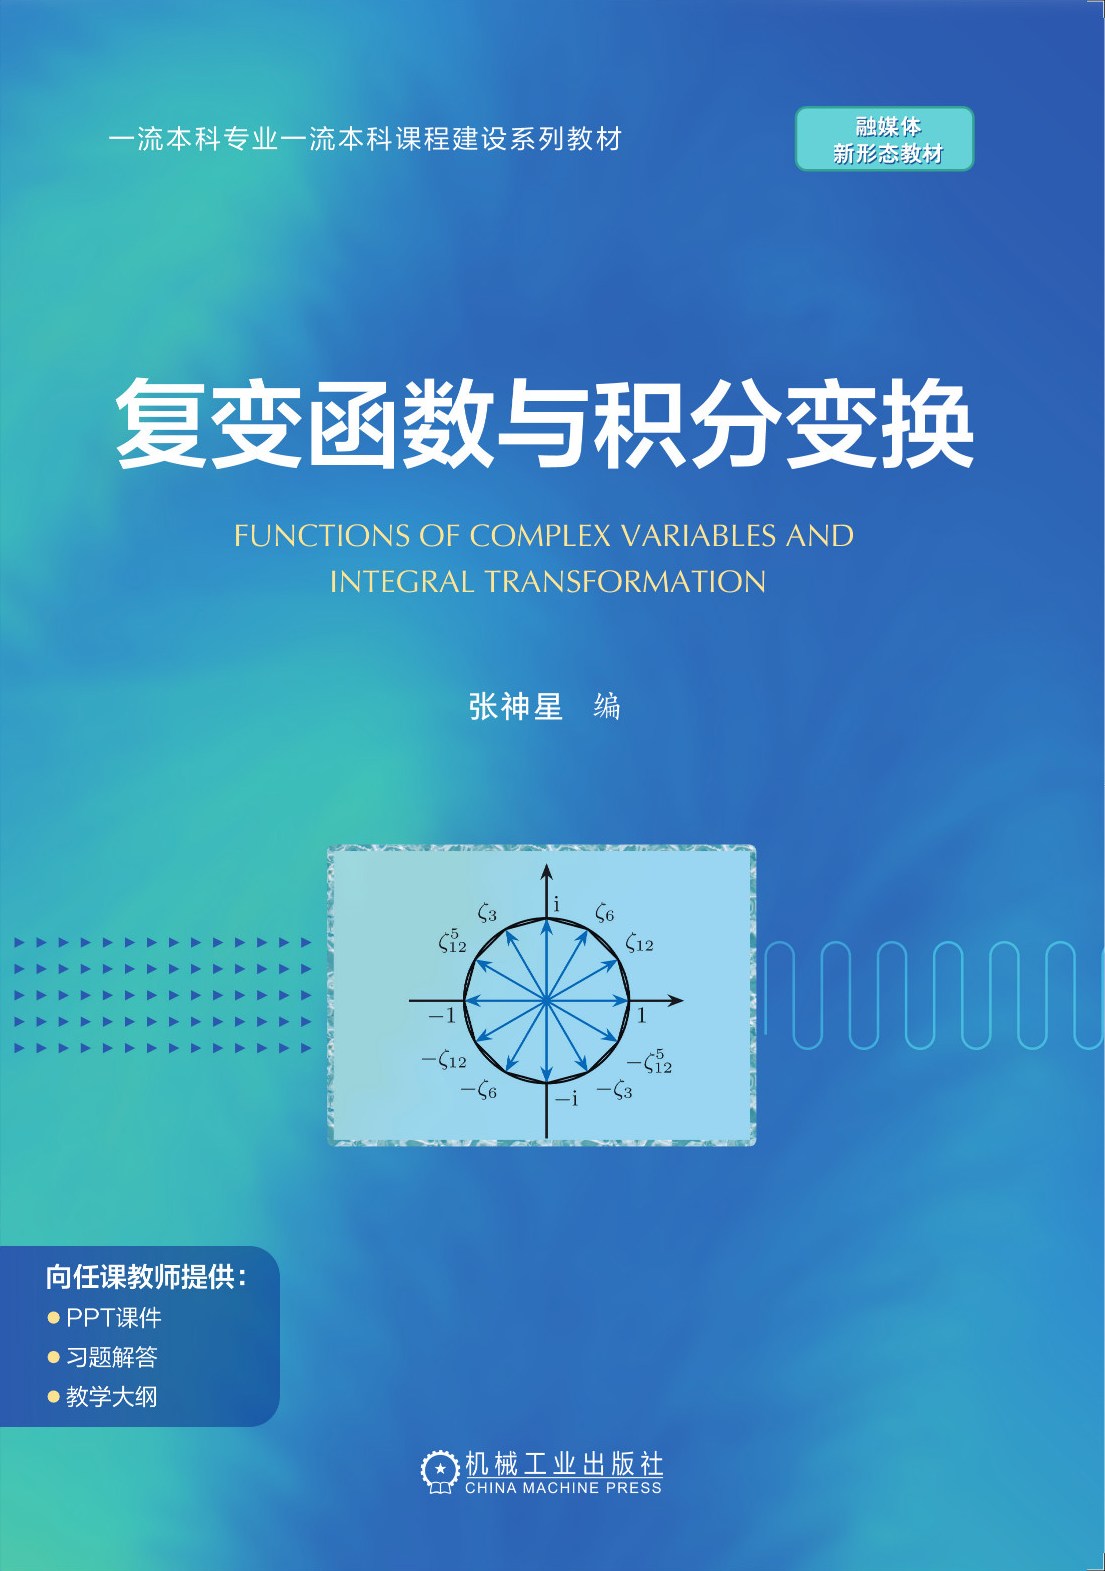
\includegraphics[height=56mm]{../image/book.png}};
	\end{tikzpicture}
\end{frame}


\begin{frame}{成绩构成}
	\vspace{-\baselineskip}
	\begin{center}
	\begin{tikzpicture}
		\begin{scope}
			\begin{scope}[xshift=.2mm,yshift=1.7mm,scale=2]
				\filldraw[cstcurve,main,cstfill1] (0,0)--(0,1) arc (90:144:1) -- cycle;
			\end{scope}
			\draw[main] (-.7,1.5)--(-1.6,2.5)--(-3,2.5);
			\filldraw[main,cstfill1] (-.7,1.5) circle(.1);
			\node at (-4.6,2) [text width=28mm]  (1){
				\begin{main}[
					title=作业 15分,
					centerbox,
					frame style={draw=none},
					borderline north={1pt}{-1pt}{main},
					borderline south={1pt}{-1pt}{main},
				]\kaishu
					作业通过超星发布和提交, 约两周交一次.
					\alert{作业必须按时提交, 不允许补交}.
				\end{main}
			};
		\end{scope}

		\begin{scope}
			\begin{scope}[xshift=1.5mm,yshift=1.7mm,scale=2]
				\filldraw[cstcurve,second,cstfill2] (0,0)--(1,0) arc (0:90:1) -- cycle;
			\end{scope}
			\draw[second] (.9,1.5)--(1.6,2.5)--(3,2.5);
			\filldraw[second,cstfill2] (.9,1.5) circle(.1);
			\node at (4.6,1.8) [text width=28mm] (2){
				\begin{second}[
					title=课堂测验 25分,
					centerbox,
					frame style={draw=none},
					borderline north={1pt}{-1pt}{second},
					borderline south={1pt}{-1pt}{second},
				]\kaishu
					课堂测验共3次, 取最高的两次平均. 测验范围和时间会提前通知. \alert{测验时在教室内作答,否则按未考处理}. 
				\end{second}
			};
		\end{scope}

		\begin{scope}
			\begin{scope}[xshift=1.8mm,yshift=.5mm,scale=1.95]
				\filldraw[cstcurve,third,cstfill3] (0,0)--({cos{36}},-sin{36}) arc (-36:0:1) -- cycle;
			\end{scope}
			\draw[third] (1.5,-.4)--(2.2,-1.1)--(3,-1.1);
			\filldraw[third,cstfill3] (1.5,-.4) circle(.1);
			\node at (4.6,-1.2) [text width=28mm] (3){
				\begin{third}[
					title=其它 10分,
					centerbox,
					frame style={draw=none},
					borderline north={1pt}{-1pt}{third},
					borderline south={1pt}{-1pt}{third},
				]\kaishu
					完成超星各个章节的任务点.
				\end{third}
			};
		\end{scope}

		\begin{scope}
			\begin{scope}[scale=2.1]
				\filldraw[cstcurve,fourth,cstfill4] (0,0)--({cos{144}},sin{144}) arc (144:324:1) -- cycle;
			\end{scope}
			\draw[fourth] (-.7,-1)--(-1.6,-1.7)--(-3,-1.7);
			\filldraw[fourth,cstfill4] (-.7,-1) circle(.1);
			\node at (-4.6,-1) [text width=28mm] (4){
				\begin{fourth}[
					title=期末考试 50分,
					centerbox,
					frame style={draw=none},
					borderline north={1pt}{-1pt}{fourth},
					borderline south={1pt}{-1pt}{fourth},
				]\kaishu
					期末卷面需要达到45分才计算总评分数, 45分以下直接不及格.
				\end{fourth}
			};
		\end{scope}
	\end{tikzpicture}
\end{center}
\end{frame}



\begin{frame}{复变函数的应用}
	\onslide<+->
	复变函数的应用非常广泛, 它包括:
	\begin{itemize}
		\item \alert{数学}中的代数、数论、几何、分析、动力系统……
		\item \alert{物理学}中流体力学、材料力学、电磁学、光学、量子力学……
		\item \alert{信息学}、\alert{电子学}、\alert{电气工程}……
	\end{itemize}
	\onslide<+->
	可以说复变函数应用之广, 在大学数学课程中仅次于高等数学和线性代数. 
\end{frame}


\begin{frame}{课程内容关系}
	\begin{center}
		\begin{tikzpicture}[node distance=18pt]
			\node[cstnode4] (1) {复数的要素};
			\node[cstnode4] (2) [right=35pt of 1] {四则运算};
			\node[cstnode4] (3) [right=32pt of 2] {幂和方根};
			
			\node[cstnode4] (11) [below=of 1] {数列极限};
			\node[cstnode4] (12) [below=of 2] {函数极限};
			\node[cstnode4] (13) [below=of 3] {连续};

			\node[cstnode4] (21) [below=of 11] {导数};
			\node[cstnode4] (22) [below=of 12] {解析函数};
			\node[cstnode2] (23) [below=of 13] {柯西-黎曼方程};
			\node[cstnode2] (24) [right=of 23] {初等函数};

			\node[cstnode2] (31) [below=of 21] {积分: 参变量法};
			\node[cstnode4] (32) [align=center,below=of 22] {柯西-古萨定理};
			\node[cstnode2] (33) [below=of 23] {原函数法};
			\node[cstnode4] (34) [below=of 24] {柯西积分公式};
			\node[cstnode2] (35) [right=of 34] {留数法};

			\node[cstnode4] (41) [below=of 32] {幂级数};
			\node[cstnode4] (42) [below=of 33] {泰勒展开};
			\node[cstnode4] (43) [below=of 34] {洛朗级数};

			\node[cstnode3] (51) [above=42pt of 24] {傅里叶变换};
			\node[cstnode3] (54) [right=88pt of 13] {拉普拉斯变换};
			\begin{scope}[cstmra,main]
				\draw (1.east) to (2.west);
				\draw (2.east) to (3.west);
				\draw (1.south) to (11.north);
				\draw (1.south) to (12.north);
				\draw (12.east) to (13.west);
				\draw (12.south) to (21.north);
				\draw (21.east) to (22.west);
				\draw (22.east) to (23.west);
				\draw (23.east) to (24.west);
				\draw (21.south) to (31.north);
				\draw (23.south) to (32.north);
				\draw (31.east) to (32.west);
				\draw (32.east) to (33.west);
				\draw (33.east) to (34.west);
				\draw (34.east) to (35.west);
				\draw (34.south) to (42.north);
				\draw (34.south) to (43.north);
				\draw (41.east) to (42.west);
				\draw (42.east) to (43.west);
				\draw (43.east) to (35.south);
				\draw (35.north) to (54.south);
				\draw (24.north) to (51.south);
			\end{scope}
		\end{tikzpicture}
	\end{center}
\end{frame}


\begin{frame}{课程学习方法}
	\begin{center}
		\begin{tikzpicture}[node distance=25pt]
			\node[cstnode4,align=center] (1) at (0,2)  {\alert{课前}\\预习课本};
			\node[cstnode4,align=center] (2) at (3,0)  {\alert{课上}\\认真听课\\记好笔记};
			\node[cstnode4,align=center] (3) at (0,-2) {\alert{课后}\\过一遍教材\\与课上知识点};
			\node[cstnode4,align=center] (4) at (-3,0) {\alert{作业}\\检测学\\习效果};
			\draw[cstnra,main] (1.east) to[bend left] (2.north);
			\draw[cstnra,main] (2.south) to[bend left] (3.east);
			\draw[cstnra,main] (3.west) to[bend left] (4.south);
			\draw[cstnra,main] (4.north) to[bend left] (1.west);
		\end{tikzpicture}
	\end{center}
\end{frame}



\part{复数与复变函数}
\section{复数及其代数运算}

\subsection{复数的产生}

\begin{frame}{复数的引入\noexer}
	\begin{itemize}
		\item 复数起源于多项式方程的求根问题.
		\item 考虑一元二次方程 $x^2+bx+c=0$.
		\item 配方可得 $\Bigl(x+\dfrac b2\Bigr)^2=\dfrac{b^2-4c}4$.
		\item 于是得到求根公式 $x=\dfrac{-b\pm\sqrt\Delta}2$, 其中 $\Delta=b^2-4c$.
		\begin{enumerate}
			\item 当 $\Delta>0$ 时, 有两个不同的实根;
			\item 当 $\Delta=0$ 时, 有一个二重的实根;
			\item 当 $\Delta<0$ 时, 无实根.
		\end{enumerate}
		\item 可以看出, 在一元二次方程中, 我们可以舍去包含\alert{负数开方}的解.
		\item 然而在一元三次方程中, 即便只考虑实数根也会不可避免地引入负数开方.
	\end{itemize}
\end{frame}



\begin{frame}{三次方程的根\noexer}
	\onslide<+->
	\begin{example}[nearnext]
		解方程 $x^3+6x-20=0$.
	\end{example}
	\onslide<+->
	\begin{solution}[nearprev,sidepic,righthand width=3.2cm,leftupper=0mm]
		\begin{itemize}
			\item 设 $x=u+v$,
			\item 那么 $u^3+v^3+3uv(u+v)+6(u+v)-20=0$.
			\item 我们希望 $u^3+v^3=20$, $uv=-2$.
			\item 那么 $u^3,v^3$ 满足一元二次方程 $X^2-20X-8=0$.
			\item 解得 $u^3=10\pm\sqrt{108}=(1\pm\sqrt3)^3$.
			\item 所以 $u=1\pm\sqrt3$, $v=1\mp\sqrt 3$.
			\item $x=u+v=2$.
		\end{itemize}
		\tcblower
		\onslide<+->{
		\begin{tikzpicture}
			\begin{scope}[xscale=.78]
				\draw[cstaxis] (-2,0)--(2,0);
				\draw[cstaxis] (0,-2)--(0,2);
				\clip (-2,-2) rectangle (2,2);
				\begin{scope}[xscale=.3,yscale=.04]
					\draw[cstcurve,main,domain=-3:4,smooth] plot (\x,{\x*\x*\x+6*\x-20});
					\coordinate (A) at (2,0);
					\coordinate (B) at (0,-20);
				\end{scope}
				\draw[inner sep=2pt]
					(A) node[below right] {$2$}
					(B) node[above left] {$-20$};
			\end{scope}
			\begin{scope}[cstdot]
				\fill (A) circle;
				\fill (B) circle;
			\end{scope}
		\end{tikzpicture}}
	\end{solution}
\end{frame}


\begin{frame}{三次方程的根\noexer}
	\beqskip{1pt}
	\onslide<+->
	\begin{example}[nearnext]
		解方程 $x^3-7x+6=0$.
	\end{example}
	\onslide<+->
	\begin{solution}[nearprev,sidepic,righthand width=2.7cm,leftupper=0mm]
		\begin{itemize}
			\item 类似地 $x=u+v$, 其中 $u^3+v^3=-6$, $uv=\frac73$.
			\item 于是 $u^3,v^3$ 满足一元二次方程 $X^2+6X+\frac{343}{27}=0$.
			\item 这个方程没有实数解, 我们可以强行解得 
		\end{itemize}
		\onslide<+->{%
		\[
			u^3=-3+\dfrac{10}9\sqrt{-3},\ 
			\visible<+->{u=\frac{3+2\sqrt{-3}}3,\frac{-9+\sqrt{-3}}6,\frac{3-5\sqrt{-3}}6,}
		\]}
		\begin{itemize}
			\item $v=\dfrac{3-2\sqrt{-3}}3,\dfrac{-9-\sqrt{-3}}6,\dfrac{3+5\sqrt{-3}}6$,
			\item $x=u+v=2,-3,1$.
		\end{itemize}
		\tcblower
		\onslide<+->{%
		\begin{tikzpicture}
			\begin{scope}[xscale=.7]
				\def\a{-3}
				\def\b{1}
				\def\c{2}
				\draw[cstaxis] (-2,0)--(2,0);
				\draw[cstaxis] (0,-2)--(0,2);
				\clip (-2,-2) rectangle (2,2);
				\begin{scope}[xscale=.45,yscale=.1]
					\draw[cstcurve,main,domain=-4:4,smooth] plot (\x,{(\x-\a)*(\x-\b)*(\x-\c)});
					\coordinate (A) at (\a,0);
					\coordinate (B) at (\b,0);
					\coordinate (C) at (\c,0);
				\end{scope}
				\draw[inner sep=2pt]
					(A) node[below right] {$-3$}
					(B) node[below left] {$1$}
					(C) node[below right] {$2$};
			\end{scope}
			\begin{scope}[cstdot]
				\fill (A) circle;
				\fill (B) circle;
				\fill (C) circle;
			\end{scope}
		\end{tikzpicture}}
	\end{solution}
	\endgroup
\end{frame}


\begin{frame}{三次方程的根\noexer}
	\begin{itemize}
		\item 一般地, 方程 $x^3+px+q=0$ 的解为($p=0$ 情形较简单, 这里不考虑)
		\[
			x=u-\frac p{3u},\quad u^3=-\frac q2+\sqrt{\Delta},\quad \Delta=\frac{q^2}4+\frac{p^3}{27}.
		\]
		\item 通过分析函数图像的极值点可以知道:
	\end{itemize}
	\begin{center}
		\begin{tikzpicture}[visible on=<3->]
			\begin{scope}[scale=.65,
				declare function={
					f(\x)=\x*\x*\x-3*\x;
				}
			]
				\def\a{2.5}
				\draw[cstaxis] (-2,0)--(2,0);
				\draw[cstaxis] (0,-2) node[below] {$\Delta>0$, 有 $1$ 个根}--(0,2);
				\clip (-2,-2) rectangle (2,2);
				\begin{scope}[xscale=.35,yscale=.1]
					\draw[cstcurve,main,domain=-3:4,smooth] plot (\x,{f(\x)-f(\a)});
					\coordinate (A) at (\a,0);
				\end{scope}
			\end{scope}
			\fill[cstdot] (A) circle;
			\begin{scope}[visible on=<4->,xshift=5cm]
				\begin{scope}[scale=.65]
					\def\a{-2}
					\def\b{1}
					\draw[cstaxis] (-2,0)--(2,0);
					\draw[cstaxis] (0,-2) node[below,align=center] {$\Delta=0$, 有 $2$ 个根\\$x=-\sqrt[3]{4q},\half\sqrt[3]{4q}$ ($2$重).}--(0,2);
					\clip (-2,-2) rectangle (2,2);
					\begin{scope}[xscale=.35,yscale=.1]
						\draw[cstcurve,main,domain=-4:3,smooth] plot ({\x},{(\x-\a)*(\x-\b)*(\x-\b)});
						\coordinate (A) at (\a,0);
						\coordinate (B) at (\b,0);
					\end{scope}
				\end{scope}
				\begin{scope}[cstdot]
					\fill (A) circle;
					\fill (B) circle;
				\end{scope}
			\end{scope}
			\begin{scope}[visible on=<5->,xshift=10cm]
				\begin{scope}[scale=.65]
					\def\a{-3}
					\def\b{.5}
					\def\c{2.5}
					\draw[cstaxis] (-2,0)--(2,0);
					\draw[cstaxis] (0,-2) node[below] {$\Delta<0$, 有 $3$ 个根}--(0,2);
					\clip (-2,-2) rectangle (2,2);
					\begin{scope}[xscale=.3,yscale=.05]
						\draw[cstcurve,main,domain=-5:5,smooth] plot ({\x},{(\x-\a)*(\x-\b)*(\x-\c)});
						\coordinate (A) at (\a,0);
						\coordinate (B) at (\b,0);
						\coordinate (C) at (\c,0);
					\end{scope}
				\end{scope}
				\begin{scope}[cstdot]
					\fill (A) circle;
					\fill (B) circle;
					\fill (C) circle;
				\end{scope}
			\end{scope}
		\end{tikzpicture}
	\end{center}
\end{frame}


\begin{frame}{三次方程的根\noexer}
	\begin{itemize}
		\item 由此可见, 若想使用求根公式, 就\alert{必须接受负数开方}.
		\item 那么为什么当 $\Delta<0$ 时, 从求根公式一定能得到 $3$ 个实根呢?
		\item 这个问题在我们学习了第一章的内容之后可以得到回答.
		\item 尽管在十六世纪, 人们已经得到了三次方程的求根公式, 然而对其中出现的虚数, 却是难以接受.
		\item 莱布尼兹曾说: {\color{third}\itshape 圣灵在分析的奇观中找到了超凡的显示, 这就是那个理想世界的端兆, 那个介于存在与不存在之间的两栖物, 那个我们称之为虚的 $-1$ 的平方根。}
		\item 不过, 现在我们可以用更为现代和严格的语言来引入复数.
	\end{itemize}
\end{frame}

\subsection{复数的概念}

\begin{frame}{复数的定义}
	\begin{itemize}
		\item 现在我们来正式介绍复数的概念.
		\item 为了避免记号 $\sqrt{-1}$ 带来的歧义, 我们先引入抽象符号 $\ii$, 再通过定义它的运算来构造复数.
	\end{itemize}
	\onslide<+->
	\begin{definition}
		固定一个记号 $\ii$, \emph{复数}就是形如 $z=x+y\ii$ 的元素, 其中 $x,y$ 均是实数, 且不同的 $(x,y)$ 对应不同的复数.
	\end{definition}
	\begin{itemize}
		\item 实数 $x$ 可以自然地看成复数 $x+0\ii$.
	\end{itemize}
\end{frame}


\begin{frame}{复平面}
	\begin{itemize}
		\item 回忆全体实数、有理数、整数、自然数构成的集合分别记作 $\BR,\BQ,\BZ,\BN$.
		\item 将\emph{全体复数记作 $\BC$}.
		\item 那么 $\BC$ 自然构成一个二维实线性空间, 且 $\{1,\ii\}$ 是一组基. 
		\item 因此它和平面上的点可以建立一一对应, 并将建立起这种对应的平面称为\emph{复平面}.
	\end{itemize}
	\onslide<+->
	\begin{center}
		\begin{tikzpicture}
			\begin{scope}
				\draw[cstaxis] (-.5,0)--(3,0);
				\draw[cstaxis] (0,-.5)--(0,2.5);
				\coordinate [label=below left:$0$] (O) at (0,0);
				\coordinate [label=above:\textcolor{second}{$z=x+y\ii$}] (A) at (2,1.5);
				\coordinate (B) at (2,0);
				\coordinate (C) at (0,1.5);
				\draw[cstdash] (B)--(A)--(C);
				\fill[cstdot,second] (A) circle;
				\draw[third,Latex-Latex,line width=.5mm] (2.8,1)--(4,1) node[midway,below,third] {一一对应};
			\end{scope}
			\begin{scope}[xshift=5cm]
				\coordinate [label=below left:$O$] (O) at (0,0);
				\coordinate [label=above:\textcolor{second}{$Z(x,y)$}] (A) at (2,1.5);
				\coordinate (B) at (2,0);
				\coordinate (C) at (0,1.5);
				\draw[cstdash] (B)--(A)--(C);
				\fill[cstdot,second] (A) circle;
				\draw[decorate,decoration={brace,amplitude=5},main,cstfill1] (O)--(B) node[midway,above=2mm] {$x$};
				\draw[decorate,decoration={brace,amplitude=5},main,cstfill1] (C)--(O) node[midway,right=2mm] {$y$};
				\draw[third,Latex-Latex,line width=.5mm] (2.8,1)--(4,1) node[midway,below,third] {一一对应};
				\draw[cstaxis] (-.5,0)--(3,0);
				\draw[cstaxis] (0,-.5)--(0,2.5);
			\end{scope}
			\begin{scope}[xshift=10cm]
				\draw[cstaxis] (-.5,0)--(3,0);
				\draw[cstaxis] (0,-.5)--(0,2.5);
				\coordinate [label=below left:$O$] (O) at (0,0);
				\coordinate [label=above:\textcolor{second}{$\overrightarrow{OZ}=(x,y)$}] (A) at (2,1.5);
				\draw[cstcurve,cstra,second] (O)--(A);
			\end{scope}
		\end{tikzpicture}
	\end{center}
\end{frame}


\begin{frame}{实部和虚部, 虚数和纯虚数}
	\onslide<+->
	\begin{itemize}
		\item $x,y$ 轴分别对应复平面的\emph{实轴}和\alert{虚轴}.
		\item 称 $z=x+y\ii$ 中 $x=\Re z$ 为 $z$ 的\emph{实部}; $y=\Im z$ 为 $z$ 的\alert{虚部}.
		\item 当虚部 $\Im z=0$ 时, $z$ 为实数, 它落在实轴上.
		\item 不是实数的复数是\textcolor{third}{\bf 虚数}.
		\item 当实部 $\Re z=0$ 且 \alert{$z\neq0$} 时, $z$ 为\alert{纯虚数}, 它落在虚轴上.
	\end{itemize}
	\onslide<1->
	\begin{figure}[hbpt]
		\centering
		\begin{minipage}{.48\textwidth}
			\raggedleft
			\begin{tikzpicture}
				\coordinate [label=below left:$0$] (O) at (0,0);
				\coordinate (B) at (2,0);
				\coordinate (C) at (0,1.5);
				\draw[cstaxis] (-.5,0)--(3,0);
				\draw[cstaxis] (0,-.5)--(0,2.5);
				\begin{scope}[visible on=<3->]
					\draw[decorate,decoration={brace,amplitude=5},main,cstfill1] (B)--(O) node[midway,below=1.5mm] {$\Re z$};
					\draw[decorate,decoration={brace,amplitude=5},second,cstfill2] (C)--(O) node[midway,right=1.5mm] {$\Im z$};
					\coordinate [label=above:\textcolor{third}{$z=x+y\ii$}] (A) at (2,1.5);
					\draw[cstdash] (B)--(A)--(C);
					\fill[cstdot,third] (A) circle;
				\end{scope}
				\begin{scope}[visible on=<2->]
					\coordinate [label=above:\textcolor{main}{实轴}] (R) at (3,0);
					\coordinate [label=right:\textcolor{second}{虚轴}] (I) at (0,2.5);
					\draw[cstaxis,main] (-.5,0)--(R);
					\draw[cstaxis,second] (0,-.5)--(I);
				\end{scope}
				\draw[main,->,thick,visible on=<4->] (-2,.2)-|(.6,0);
				\draw[second,->,thick,visible on=<6->] (-2,1.3)--(0,1.3);
				\draw 
					(-2,.1) node[cstnode,draw=main,text=main,visible on=<4->] {实数}
					(-2,1.2) node[align=center,cstnode,draw=second,text=second,visible on=<6->] {纯虚数\\不含原点};
			\end{tikzpicture}
		\end{minipage}
		\begin{minipage}{.48\textwidth}
			\centering
			\begin{tikzpicture}
				\filldraw[cstcurve,cstfill] (.8,0) circle (2.6 and 2);
				\coordinate (R) at (0,-.8);
				\filldraw[cstcurve,main,fill=white,visible on=<4->] (R) circle (1.2 and .7);
				\coordinate (I) at (0,.8);
				\draw (R) node[align=center,main,visible on=<4->] {实数 \\$0,1,\sqrt2,\pi,\ee$};
				\draw (I) node[align=center,second,visible on=<6->] {纯虚数 \\$\ii,-\ii ,\pi\ii$};
				\draw[cstcurve,second,visible on=<6->] (I) circle (1.2 and .7);
				\draw 
					(3.7,0) node[align=center] {全\\体\\复\\数}
					(2,0) node[align=center,third,visible on=<5->] {虚数 \\$\ii,\pi\ii,\frac{-1+\sqrt 3 \ii}2$};
			\end{tikzpicture}
		\end{minipage}
	\end{figure}
\end{frame}


\begin{frame}{例题:判断实数和纯虚数}
	\onslide<+->
	\begin{example}[nearnext]
		实数 $x$ 取何值时, $z=(x^2+3x-4)+(x^2+5x-6)\ii$ 是:
		\begin{subexample}[2]
			\item 实数;
			\item 纯虚数.
		\end{subexample}
	\end{example}
	\onslide<+->
	\begin{solution}[nearprev]
		\begin{enumerate}
			\item $\Im z=x^2+5x-6=0$, 即 $x=1$ 或 $-6$.
			\item $\Re z=x^2+3x-4=0$, 即 $x=1$ 或 $-4$.
				\onslide<+->{%
					但同时要求 $\Im z=x^2+5x-6\neq 0$, 因此 $x\neq 1$.
				}\onslide<+->{%
					故 $x=-4$.
				}
		\end{enumerate}
	\end{solution}
	\onslide<+->
	\begin{exercise}
		若 $x^2(1+\ii)-x(5+4\ii)+4+3\ii$ 是纯虚数, 则实数 $x=$\fillblankframe{$4$}.
	\end{exercise}
\end{frame}


\subsection{复数的代数运算}


\begin{frame}{复数的加法与减法}
	\begin{itemize}
		\item 设 $z_1=x_1+y_1\ii,z_2=x_2+y_2\ii$.
		\item 定义复数的\emph{加法}和\emph{减法}:
		\[
			z_1+z_2=(x_1+x_2)+(y_1+y_2)\ii,\quad
			z_1-z_2=(x_1-x_2)+(y_1-y_2)\ii.
		\]
		\item 复数的加减法与其对应的向量 $\overrightarrow{OZ}$ 的加减法是一致的.
	\end{itemize}
	\onslide<1->
	\begin{center}
		\begin{tikzpicture}[scale=.7]
			\draw[cstaxis] (-2,0)--(4,0);
			\draw[cstaxis] (0,-3)--(0,2.5);
			\coordinate (O) at (0,0);
			\coordinate [label=right:\textcolor{main}{$z_1$}] (Z1) at (2.5,-1);
			\coordinate [label=above:\textcolor{main}{$z_2$}] (Z2) at (1.5,2);
			\begin{scope}[visible on=<3->]
				\coordinate [label=above right:\textcolor{second}{$z_1+z_2$}] (P) at ($(Z1)+(Z2)$);
				\draw[cstcurve,cstra,second] (O)--(P);
				\draw[cstdash] (Z2)--(P)--(Z1);
			\end{scope}
			\begin{scope}[visible on=<4->]
				\coordinate [label=below:\textcolor{third}{$z_1-z_2$}] (M) at ($(Z1)-(Z2)$);
				\coordinate [label=left:{$-z_2$}] (neg) at ($(O)-(Z2)$);
				\draw[cstcurve,cstra,third] (O)--(M);
				\draw[cstdash,cstra] (O)--(neg);
				\draw[cstdash] (Z1)--(M)--(neg);
			\end{scope}
			\draw[cstcurve,cstra,main] (O)--(Z1);
			\draw[cstcurve,cstra,main] (O)--(Z2);
		\end{tikzpicture}
	\end{center}
\end{frame}


\begin{frame}{复数的乘除法}
	\begin{itemize}
		\item \alert{规定 $\ii\cdot \ii=-1$}.
		\item 定义复数的\emph{乘法}:
		\begin{align*}
			z_1\cdot z_2&
			=(x_1+y_1\ii)(x_2+y_2\ii)
			=x_1\cdot x_2+x_1\cdot y_2\ii+y_1\ii\cdot x_2+y_1\ii\cdot y_2\ii\\
			&=(x_1x_2-y_1y_2)+(x_1y_2+x_2y_1)\ii.
		\end{align*}
		\item 此时加法/乘法交换律, 结合律以及乘法分配律均成立.
		\item 待定系数可得复数的\emph{除法}定义为:
		\[
			\frac{z_1}{z_2}
			=\frac{(x_1+y_1\ii)(x_2-y_2\ii)}{x_2^2+y_2^2}
			=\frac{x_1x_2+y_1y_2}{x_2^2+y_2^2}+\frac{x_2y_1-x_1y_2}{x_2^2+y_2^2}\ii.
		\]
		\item 对于正整数 $n$, 定义 $z$ 的 \emph{$n$ 次幂}为 $n$ 个 $z$ 相乘.
		\item 当 $z\neq 0$ 时, 还可以定义 $z^0=1,z^{-n}=\dfrac1{z^n}$.
	\end{itemize}
\end{frame}


\begin{frame}{例: 单位根}
	\onslide<+->
	\begin{example}
		\begin{enumerate}
			\item $\ii^2=-1,\ii^3=-\ii ,\ii^4=1$.
			\onslide<+->{%
			一般地, 对于整数 $n$, 
			\[
				\ii^{4n}=1,\quad \ii^{4n+1}=i,\quad
				\ii^{4n+2}=-1,\quad \ii^{4n+3}=-\ii.
			\]
			}
			\vspace{-\baselineskip}
			\item 令 $\omega=\dfrac{-1+\sqrt 3\ii}2$, 则 $\omega^2=\dfrac{-1-\sqrt3\ii}2,\omega^3=1$.
			\item 令 $z=1+\ii$, \onslide<+->{则
			\[
				z^2=2\ii,\quad z^3=-2+2\ii,\quad z^4=-4,\quad z^8=16=2^4.
			\]}
		\end{enumerate}
		\bigdel\bigdel
	\end{example}
	\begin{itemize}
		\item 将满足 $z^n=1$ 的复数 $z$ 称为 \emph{$n$ 次单位根}.
		\item 那么 $1,\ii,-1,-\ii $ 是 $4$ 次单位根, $1,\omega,\omega^2$ 是 $3$ 次单位根, $-\omega$ 是 $6$ 次单位根.
	\end{itemize}
\end{frame}


\begin{frame}{例: 代数式的计算}
	\begin{itemize}
		\item 实数情形的等差数列求和公式、等比数列求和公式、二项式展开、平方差公式等在复数情形也成立.
	\end{itemize}
	\onslide<+->
	\begin{example}[nearnext]
		化简 $1+\ii+\ii^2+\dots+\ii^{1000}$.
	\end{example}
	\onslide<+->
	\begin{solution}[nearprev]
		根据等比数列求和公式, $1+\ii+\ii^2+\dots+\ii^{1000}
			=\dfrac{\ii^{1001}-1}{\ii-1}
			\visible<+->{=\dfrac{\ii-1}{\ii-1}=1.}$
	\end{solution}
	\onslide<+->
	\begin{exercise}
		化简 $\Bigl(\dfrac{1+\ii}{1-\ii}\Bigr)^{2026}$=\fillblankframe{$-1$}.
	\end{exercise}
\end{frame}


\subsection{共轭复数}


\begin{frame}{共轭复数的定义}
	\onslide<+->
	\begin{definition}
		称 $z$ 在复平面关于实轴的对称点为它的\emph{共轭复数 $\ov z$}.
		换言之, $\ov{x+y\ii}=x-y\ii$.
	\end{definition}
	\onslide<+->
	\begin{exercise}
		$z$ 关于虚轴的对称点是\fillblankframe{$-\ov z$}.
	\end{exercise}
\end{frame}

\begin{frame}{共轭复数的性质}
	\begin{itemize}
		\item 从定义出发, 不难验证共轭复数满足如下性质:
		\begin{enumerate}\bf
			\item $z$ 是 $\ov z$ 的共轭复数.\hfill\alert{共轭是一种对合}
			\item $\ov{z_1\pm z_2}=\ov{z_1}\pm\ov{z_2},\ 
			\ov{z_1\cdot z_2}=\ov{z_1}\cdot\ov{z_2},\ 
			\ov{\Bigl(\dfrac{z_1}{z_2}\Bigr)}=\dfrac{~\ov{z_1}~}{~\ov{z_2}~}$.
			\hfill \alert{共轭复数和四则运算交换}
			\item $z\ov{z}=(\Re z)^2+(\Im z)^2$.
			\item $z+\ov z=2\Re z,\ z-\ov z=2\ii\Im z$.
			\hfill \alert{$x,y$ 和 $z,\ov z$ 可相互表示}
			\item $z=\ov z\iff z$ 是实数; $z=-\ov z\iff z$ 是纯虚数或 $z=0$.\hfill\alert{判断实数和纯虚数}
		\end{enumerate}
		\item 这些性质意味着使用共轭复数进行计算和证明,往往比直接使用 $x,y$ 表达的形式更简单.
	\end{itemize}
\end{frame}


\begin{frame}{例题:共轭复数证明等式}
	\onslide<+->
	\begin{example}
		证明 $z_1\cdot\ov{z_2}-\ov{z_1}\cdot z_2=2\ii\Im(z_1\cdot\ov{z_2})$.
	\end{example}
	\onslide<+->
	我们可以设 $z_1=x_1+y_1\ii,z_2=x_2+y_2\ii$, 然后代入等式两边化简并比较实部和虚部得到.
	\onslide<+->
	但我们利用共轭复数可以更简单地证明它.
	\onslide<+->
	\begin{proof}[leftupper=0mm]
		\begin{itemize}
			\item 由于 $\ov{z_1\cdot\ov{z_2}}=\ov{z_1}\cdot\ov{\ov{z_2}}=\ov{z_1}\cdot z_2$, 
			\item 因此
			\[
				z_1\cdot\ov{z_2}-\ov{z_1}\cdot z_2
				=z_1\cdot\ov{z_2}-\ov{z_1\cdot\ov{z_2}}
				=2\ii\Im(z_1\cdot\ov{z_2}).\qedhere
			\]
		\end{itemize}
	\end{proof}
\end{frame}


\begin{frame}{例题:共轭复数判断实数}
	\onslide<+->
	\begin{example}[nearnext]
		设 $z=x+y\ii$ 是虚数.
		证明: $x^2+y^2=1$ 当且仅当 $z+\dfrac 1z$ 是实数.
	\end{example}
	\onslide<+->
	\begin{proof}[nearprev,leftupper=0mm]
		\begin{itemize}
			\item $z+\dfrac 1z$ 是实数等价于
				$z+\dfrac 1z=\ov{\Bigl(z+\dfrac 1z\Bigr)}=\ov z+\dfrac1{~\ov z~}$,
			\item 等价于
			\[
				z-\ov z=\frac1{~\ov z~}-\frac1z=\frac{z-\ov z}{z\ov z},\quad (z-\ov z)(z\ov z-1)=0.
			\]
			\item 由 $z$ 是虚数可知 $z\neq \ov z$.
			\item 故上述等式等价于 $z\ov z=1$, 即 $x^2+y^2=1$.\qedhere
		\end{itemize}
	\end{proof}
\end{frame}


\begin{frame}{例: 复数的代数计算}
	\onslide<+->
	由于 $z\ov z$ 是一个实数,
	\onslide<+->
	因此在做复数的除法运算时, 可以利用下式将其转化为乘法:
	\[
		\dfrac{z_1}{z_2}=\dfrac{z_1\ov{z_2}}{z_2\ov{z_2}}=\dfrac{z_1\ov{z_2}}{x_2^2+y_2^2}.
	\]
	\bigdel
	\onslide<+->
	\begin{example}[nearnext]
		$z=-\dfrac1\ii-\dfrac{3\ii}{1-\ii }$, 求 $\Re z,\Im z$ 以及 $z\ov z$.
	\end{example}
	\onslide<+->
	\begin{solution}[nearprev]
		\[
			z=-\frac1\ii-\frac{3\ii}{1-\ii }
			\onslide<+->{=\ii-\frac{3\ii-3}2=\frac32-\half \ii,}
		\]
		\onslide<+->{%
		\[
			\Re z=\frac32,\quad\Im z=-\half ,\quad
			z\ov z=\Bigl(\frac32\Bigr)^2+\Bigl(-\half\Bigr)^2=\frac52.
		\]
		}
		\bigdel
	\end{solution}
\end{frame}


\begin{frame}{例: 复数的代数计算}
	\onslide<+->
	\begin{example}[nearnext]
		设 $z_1=5-5\ii,z_2=-3+4\ii$, 求 $\ov{\Bigl(\dfrac{z_1}{z_2}\Bigr)}$.
	\end{example}
	\onslide<+->
	\begin{solution}[nearprev]
		\begin{align*}
			\frac{z_1}{z_2}&=\frac{5-5\ii}{-3+4\ii}
			\onslide<+->{=\frac{(5-5\ii)(-3-4\ii)}{(-3)^2+4^2}}\\
			&\onslide<+->{=\frac{(-15-20)+(-20+15)\ii}{25}}
			\onslide<+->{=-\frac75-\frac15\ii,}
		\end{align*}
		\onslide<+->{%
			因此 $\ov{\Bigl(\dfrac{z_1}{z_2}\Bigr)}=-\dfrac75+\dfrac15\ii$.
		}
	\end{solution}
\end{frame}



% \begin{frame}{复数域\noexer}
% 	\begin{itemize}
% 		\item 复数全体构成一个\emph{域}.
% 		\item 所谓的域, 是指带有如下内容和性质的集合
% 		\begin{itemize}\bf
% 			\item 包含 $0,1$, 且有四则运算;
% 			\item 满足加法结合/交换律, 乘法结合/交换/分配律;
% 			\item 对任意 $a$, $a+0=a\times 1=a$.
% 		\end{itemize}
% 		\item 有理数全体 $\BQ$, 实数全体 $\BR$ 也构成域, 它们是 $\BC$ 的子域.
% 		\item 与有理数域和实数域有着本质不同的是, 复数域是\emph{代数闭域}:
% 		\item 对于任何次数 $n\ge 1$ 的复系数多项式
% 		\[
% 			p(z)=z^n+c_{n-1}z^{n-1}+\cdots+c_1z+c_0,
% 		\]
% 		都存在复数 $z_0$ 使得 $p(z_0)=0$.
% 		\item 由此不难知道, 复系数多项式可以因式分解成一次多项式的乘积.
% 		\item 我们会在第五章证明该结论.
% 	\end{itemize}
% \end{frame}


% \begin{frame}{复数域不是有序域\noexer}
% 	\begin{itemize}
% 		\item \onslide<+->
% 	\end{itemize}
% 	在 $\BQ,\BR$ 上可以定义出一个好的大小关系,
% 	\onslide<+->
% 	换言之它们是有序域, 即存在一个满足下述性质的 $>$:
% 	\begin{itemize}\bf
% 		\item 若 $a\neq b$, 则要么 $a>b$, 要么 $b>a$;
% 		\item 若 $a>b$, 则对于任意 $c$, $a+c>b+c$;
% 		\item 若 $a>b,c>0$, 则 $ac>bc$.
% 	\end{itemize}
% 	\onslide<+->
% 	而 \alert{$\BC$ 却不是有序域}.
% 	\onslide<+->
% 	如果 $\ii>0$, 则
% 	\[
% 		-1=\ii\cdot \ii>0,\quad -\ii =-1\cdot \ii>0.
% 	\]
% 	\onslide<+->
% 	于是 $0>\ii$, 矛盾! 同理 $\ii<0$ 也不可能.
% \end{frame}

\section{复数的三角形式与指数形式}


\subsection{复数的模和辐角}


\begin{frame}{复数的极坐标形式}
	\onslide<+->
	由平面的极坐标表示, 我们可以得到复数的另一种表示方式.
	\onslide<+->
	以 $0$ 为极点, 正实轴为极轴, 逆时针为极角方向可以定义出复平面上的极坐标系.
	\onslide<4->{
	\begin{definition}
		\begin{enumerate}
			\item 称 $r$ 为 $z$ 的\emph{模}, 记为 \emph{$\abs{z}=r$}.
			\item<5-> 称 $\theta$ 为 $z$ 的\emph{辐角}, 记为 \emph{$\Arg z=\theta$}.
			\onslide<6->{约定 \alert{$0$ 的辐角没有定义}.}
		\end{enumerate}
	\end{definition}}
	\onslide<2->
	\begin{twopart}[nearprev]{185pt}
		\begin{center}
			\begin{tikzpicture}[scale=.8]
				\coordinate [label=below left:$0$] (O) at (0,0);
				\coordinate [label=above:\textcolor{second}{$z=x+y\ii$}] (Z) at (3,2);
				\coordinate (X) at (3,0);
				\coordinate (Y) at (0,2);
				\draw[decorate,decoration={brace,amplitude=5},main,cstfill1] (X)--(O) node[midway,below=2mm] {$x$};
				\draw[decorate,decoration={brace,amplitude=5},main,cstfill1] (O)--(Y) node[midway,left=2mm] {$y$};
				\draw[third,thick,cstra] pic [cstfill3,draw=third, "$\theta$", angle eccentricity=1.3, angle radius=0.8cm] {angle=X--O--Z};
				\draw[cstaxis] (-.5,0)--(4,0);
				\draw[cstaxis] (0,-.5)--(0,3);
				\draw[cstcurve,third,cstra] (O)--(Z) node[midway,above,third] {$r$};
				\draw[cstdash] (X)--(Z)--(Y);
				\fill[cstdot,second] (Z) circle;
			\end{tikzpicture}
		\end{center}
		\tcblower
		\begin{center}
			\onslide<3->{
			\[
				x=r\cos\theta,\qquad y=r\sin\theta,
			\]
			\[
				r=\sqrt{x^2+y^2}.
			\]}
		\end{center}
	\end{twopart}
\end{frame}


\begin{frame}{辐角主值}
	\onslide<+->
	任意非零复数 $z$ 都有无穷多个辐角.
	\onslide<+->
	称其中位于 $(-\pi,\pi]$ 的那个辐角为\emph{辐角主值}或\emph{主辐角}, 记作 $\emphm{\arg z}$.
	\onslide<+->
	那么
	\[
		\emphm{\Arg z=\arg z+2k\pi, k\in\BZ}.
	\]
	\onslide<8->
	注意 \alert{$\arg \ov z=-\arg z$ 未必成立}, 当且仅当 $z$ 不是负实数和 $0$ 时该等式成立.
	\onslide<2->
	\begin{twopart}[near]{203pt}
		\smalldel
		\onslide<4->{
		\[
			\arg z=\begin{cases}
				\visible<4->{\emphn{\arctan\dfrac yx,}}&\visible<4->{\emphn{x>0;}}\medskip\\
				\visible<5->{\alertn{\arctan\dfrac yx+\pi,}}&\visible<5->{\alertn{x<0,y\ge0;}}\medskip\\
				\visible<6->{\color{third}{\arctan\dfrac yx-\pi,}}&\visible<6->{\color{third}{x<0,y<0;}}\\
				\visible<7->{\color{fourth}{\dfrac\pi2,}}&
				\visible<7->{\color{fourth}{x=0,y>0;}}\\
				\visible<7->{\color{fourth}{-\dfrac\pi2,}}&
				\visible<7->{\color{fourth}{x=0,y<0.}}
			\end{cases}
		\]}\bigdel
		\tcblower\smalldel
		\begin{center}
			\begin{tikzpicture}
				\draw[cstaxis](-2.5,0)->(2.5,0); 
				\draw[cstaxis](0,-2)->(0,2);
				\draw[cstaxis,main,cstwla] (-1.5,0) arc(180:-180:1.5);
				\filldraw[cstdote,draw=main] (-1.5,-.07) circle;
				\begin{scope}[visible on=<4->]
					\coordinate [label=above:\textcolor{main}{$0$}] (A) at (1.7,0);
					\fill[cstdot,main] (A) circle;
					\coordinate [label=above right:\textcolor{main}{$\arctan\dfrac yx$}] (B) at (.9,.9);
					\fill[cstdot,main] (B) circle;
					\coordinate [label=right:\textcolor{main}{$\arctan\dfrac yx$}] (C) at (1.4,-.9);
					\fill[cstdot,main] (C) circle;
				\end{scope}
				\begin{scope}[visible on=<5->]
					\coordinate [label=above left:\textcolor{second}{$\arctan\dfrac yx+\pi$}] (D) at (-1.1,.8);
					\fill[cstdot,second] (D) circle;
					\coordinate [label=below:\textcolor{second}{$\pi$}] (E) at (-.9,0);
					\fill[cstdot,second] (E) circle;
				\end{scope}
				\begin{scope}[visible on=<6->]
					\coordinate [label=left:\textcolor{third}{$\arctan\dfrac yx-\pi$}] (F) at (-1.6,-.7);
					\fill[cstdot,third] (F) circle;
				\end{scope}
				\begin{scope}[visible on=<7->]
					\coordinate [label=left:\textcolor{fourth}{$\dfrac\pi2$}] (G) at (0,.5);
					\fill[cstdot,fourth] (G) circle;
					\coordinate [label=right:\textcolor{fourth}{$-\dfrac\pi2$}] (H) at (0,-.6);
					\fill[cstdot,fourth] (H) circle;
				\end{scope}
			\end{tikzpicture}
		\end{center}\bigdel
	\end{twopart}
\end{frame}


\begin{frame}{复数模的性质}\small
	\onslide<+->
	复数的模满足如下性质
	\begin{twopart}{173pt}
		\begin{center}
			\begin{tikzpicture}[visible on=<3->,scale=.75]
				\draw[cstaxis] (-4,0)--(4.3,0);
				\draw[cstaxis] (0,-3)--(0,3);
				\coordinate (O) at (0,0);
				\coordinate (Z) at (-2.5,1.5);
				\coordinate (R) at (-2.5,0);
				\draw[decorate,decoration={brace,amplitude=5},main,cstfill1] (O)--(R) node[midway,below=2mm,main] {$\abs{\Re z}$};
				\draw[decorate,decoration={brace,amplitude=5},main,cstfill1] (R)--(Z) node[midway,left=2mm,main] {$\abs{\Im z}$};
				\draw[cstcurve,second] (O)--(Z) node[midway,above,second] {$\abs{z}$};
				\draw[cstcurve,main] (Z)--(R)--(O);
				\draw[thick] (R) ++(0,.3)--++(.3,0)--++(0,-.3);
		
				\begin{scope}[visible on=<4->]
					\coordinate [label=below right:\textcolor{main}{$z_1$}] (Z1) at (2.8,-.4);
					\coordinate (Z2) at (1.2,2);
					\coordinate [label=above right:\textcolor{main}{$z_1+z_2$}] (P) at ($(Z1)+(Z2)$);
					\coordinate [label=below:\textcolor{third}{$z_1-z_2$}] (M) at ($(Z1)-(Z2)$);
					\draw[decorate,decoration={brace,amplitude=5},main] (Z1)--(O) node[midway,below,sloped] {$\abs{z_1}$};
					\draw[decorate,decoration={brace,amplitude=5},main] (P)--(Z1) node[midway,below,sloped] {$\abs{z_2}$};
					\draw[decorate,decoration={brace,amplitude=5},second] (O)--(P) node[midway,above,sloped] {$\abs{z_1+z_2}$};
					\draw[decorate,decoration={brace,amplitude=5},main] (Z1)--(M) node[midway,below,sloped] {$\abs{z_2}$};
					\draw[decorate,decoration={brace,amplitude=5},third] (M)--(O) node[midway,below,sloped] {$\abs{z_1-z_2}$};
					\begin{scope}[cstcurve,cstra]
						\draw[main] (O)--(Z1);
						\draw[main] (Z1)--(P);
						\draw[second] (O)--(P);
						\draw[third] (O)--(M);
						\draw[main] (Z1)--(M);
					\end{scope}
				\end{scope}
				\begin{scope}[visible on=<5->]
					\coordinate (A) at (2.7,2.4);
					\draw[decorate,decoration={brace,amplitude=5},main] (A)--(P) node[midway,above,sloped] {$\abs{z_3}$};
					\draw[decorate,decoration={brace,amplitude=5},fourth] (O)--(A) node[midway,above=2mm,sloped] {$\abs{z_1+z_2+z_3}$};
					\begin{scope}[cstcurve,cstra]
						\draw[main] (P)--(A);
						\draw[fourth] (O)--(A);
					\end{scope}
				\end{scope}
			\end{tikzpicture}
		\end{center}
		\tcblower
		\begin{enumerate}\bf
			\item $z\ov z=\abs{z}^2=\abs{\ov z}^2$;
			\item $\abs{\Re z},\abs{\Im z}\le \abs{z}\le\abs{\Re z}+\abs{\Im z}$;
			\item $\bigabs{\abs{z_1}-\abs{z_2}}\le\abs{z_1\pm z_2}\le\abs{z_1}+\abs{z_2}$;
			\item $\abs{z_1+z_2+\cdots+z_n}\le\abs{z_1}+\abs{z_2}+\cdots+\abs{z_n}$.
		\end{enumerate}
	\end{twopart}
\end{frame}


\begin{frame}{例题:共轭复数解决模的等式}
	\beqskip{4pt}
	\onslide<1->{
	\begin{example}[nearnext]
		证明
		\begin{subexample}[2]
			\item $\abs{z_1z_2}=\abs{z_1\ov{z_2}}=\abs{z_1}\cdot\abs{z_2}$;
			\item $\abs{z_1+z_2}^2=\abs{z_1}^2+\abs{z_2}^2+2\Re(z_1\ov{z_2})$.
		\end{subexample}
	\end{example}}
	\onslide<+->
	\begin{proof}[nearprev]
		\begin{enumerate}
			\item 因为
			\[
				\abs{z_1z_2}^2=z_1z_2\cdot\ov{z_1}\ov{z_2}
				\onslide<+->{=z_1\ov{z_1}\cdot z_2\ov{z_2}}
				\onslide<+->{=\abs{z_1}^2\cdot\abs{z_2}^2,}
			\]
			\onslide<+->{%
				所以 $\abs{z_1z_2}=\abs{z_1}\cdot\abs{z_2}$.
			}\onslide<+->{%
				因此 $\abs{z_1\ov{z_2}}=\abs{z_1}\cdot\abs{\ov{z_2}}=\abs{z_1}\cdot\abs{z_2}$.
			}
			\item 因为
			\begin{align*}
				\text{左边}&=(z_1+z_2)(\ov{z_1}+\ov{z_2})
				=z_1\ov{z_1}+z_2\ov{z_2}+z_1\ov{z_2}+\ov{z_1}z_2,\\
				\onslide<+->{\text{右边}}&\onslide<.->{=z_1\ov{z_1}+z_2\ov{z_2}+z_1\ov{z_2}+\ov{z_1\ov{z_2}},}
			\end{align*}
			\onslide<+->{%
				而 $\ov{z_1\ov{z_2}}=\ov{z_1}z_2$, 所以两侧相等.\qedhere
			}
		\end{enumerate}
	\end{proof}
	\endgroup
\end{frame}


\subsection{复数的三角和指数形式}


\begin{frame}{复数的三角和指数形式}
	\onslide<+->
	由 $x=r\cos\theta,y=r\sin\theta$ 可得
	\onslide<+->
	\begin{definition*}[][复数的三角形式]
	\[
		z=r(\cos\theta+\ii\sin\theta).
	\]
	\end{definition*}
	\onslide<+->
	定义 \alert{$\ee^{\ii\theta}=\exp(\ii\theta):=\cos\theta+\ii\sin\theta$} (欧拉恒等式).
	\onslide<+->
	那么我们得到
	\begin{definition*}[][复数的指数形式]
	\[
		z=r\ee^{\ii\theta}=r\exp(\ii\theta).
	\]
	\end{definition*}
	\onslide<+->
	这两种形式的等价的, 指数形式可以认为是三角形式的一种缩写方式.
	\onslide<+->
	求复数的三角和指数形式的\alert{关键在于计算模和辐角}.
\end{frame}


\begin{frame}{例题: 求复数的三角和指数形式}
	\onslide<+->
	\begin{example}[nearnext]
		将 $z=-\sqrt{12}-2\ii$ 化成三角形式和指数形式.
	\end{example}
	\onslide<+->
	\begin{solution}[nearprev]
		$r=\abs{z}=\sqrt{12+4}=4$.
		\onslide<+->{%
			由于 $z$ 在第三象限,
		}\onslide<+->{%
			因此
			\[
				\arg z=\arctan\frac{-2}{-\sqrt{12}}-\pi
				\onslide<+->{=\frac\pi6-\pi=-\frac{5\pi}6.}
			\]
		}\onslide<+->{%
			故
			\[
				z=4\biggl(\cos\Bigl(-\frac{5\pi}6\Bigr)+\ii\sin\Bigl(-
				\frac{5\pi}6\Bigr)\biggr)
				=4\ee^{-\frac{5\pi\ii}6}.
			\]
		}
		\meddel
	\end{solution}
\end{frame}


\begin{frame}{例题: 求复数的三角和指数形式}
	\beqskip{10pt}
	\onslide<+->
	\begin{example}[nearnext]
		将 $z=\sin\dfrac\pi5+\ii\cos\dfrac\pi5$ 化成三角形式和指数形式.
	\end{example}
	\onslide<+->
	\begin{solution}[nearprev]
		$r=\abs{z}=1$.
		\onslide<+->{%
			由于 $z$ 在第一象限, 因此
			\[
				\arg z
				=\arctan\frac{\cos(\pi/5)}{\sin(\pi/5)}
				\onslide<+->{=\arctan\cot\frac\pi 5}
				\onslide<+->{=\frac\pi2-\frac\pi5
				=\frac{3\pi}{10}.}
			\]
		}\onslide<+->{%
			\[
				z=\cos\frac{3\pi}{10}+\ii\sin\frac{3\pi}{10}=\ee^{\frac{3\pi\ii}{10}}.
			\]
		}\bigdel
	\end{solution}
	\onslide<+->
	求复数的三角或指数形式时, 只需取一个辐角就可以了, 不要求必须是辐角主值.
	\endgroup
\end{frame}


\begin{frame}{例题: 求复数的三角和指数形式}
	\onslide<+->
	\begin{solution}[][另解]
		\[
			z=\sin\frac\pi5+\ii\cos\frac\pi5
			\visible<+->{=\cos\Bigl(\frac\pi2-\frac\pi5\Bigr)+\ii\sin\Bigl(\frac\pi2-\frac\pi5\Bigr)}
			\visible<+->{=\cos\frac{3\pi}{10}+\ii\sin\frac{3\pi}{10}=\ee^{\frac{3\pi\ii}{10}}.}
		\]
		\bigdel
	\end{solution}
	\onslide<+->
	\begin{exercise}[nearnext]
		将 $z=\sqrt 3-3\ii$ 化成三角形式和指数形式.
	\end{exercise}
	\onslide<+->
	\begin{answer}[nearprev]
		$\displaystyle z=2\sqrt3\biggl(\cos\Bigl(-\frac{\pi}3\Bigr)+\ii\sin\Bigl(-\frac{\pi}3\Bigr)\biggr)
		=2\sqrt3 \ee^{-\frac{\pi\ii}3}$, 写成 $\dfrac{5\pi}3$ 也可以.
	\end{answer}
\end{frame}


\begin{frame}{模为 $1$ 的复数}
	\onslide<+->
	两个模相等的复数之和的三角和指数形式形式较为简单.
	\onslide<+->
	\begin{twopart}{180pt}
		\[
			\ee^{\ii\theta}+\ee^{\ii\varphi}
			=2\cos\frac{\theta-\varphi}2\ee^{\frac{\theta+\varphi}2\ii}.
		\]
		\tcblower
		\begin{center}
			\begin{tikzpicture}[scale=.75]
				\coordinate [label=below left:0] (O) at (0,0);
				\coordinate [label=right:\textcolor{main}{$\ee^{\ii\varphi}$}] (Z1) at ({3*cos(18)},{3*sin(18)});
				\coordinate [label=left:\textcolor{main}{$\ee^{\ii\theta}$}] (Z2) at ({3*cos(130)},{3*sin(130)});
				\coordinate [label=above right:\textcolor{second}{$\ee^{\ii\theta}+\ee^{\ii\varphi}$}] (P) at ($(Z1)+(Z2)$);
				\coordinate (M) at ($0.5*(P)$);
				\coordinate (X) at (2,0);
				\draw[thick,main] pic [cstfill1, draw=main,"$\varphi$", angle eccentricity=1.4, angle radius=0.7cm] {angle=X--O--Z1};
				\draw[thick,second] pic [cstfill2, draw=second, "$\frac{\theta-\varphi}2$", angle eccentricity=1.7] {angle=Z1--O--P};
				\draw[cstaxis] (-3,0)--(3,0);
				\draw[cstaxis] (0,-.4)--(0,3.5);
				\draw[cstcurve,cstra,main] (O)--(Z1);
				\draw[cstcurve,cstra,main] (O)--(Z2);
				\draw[cstcurve,cstra,second] (O)--(P);
				\draw[cstdash] (Z2)--(Z1)--(P)--(Z2);
				\draw[thick] (M)--++({.3*cos(16)},{-.3*sin(16)})--++({.3*sin(16)},{.3*cos(16)})--++({-.3*cos(16)},{.3*sin(16)});
			\end{tikzpicture}
		\end{center}
	\end{twopart}
	\onslide<+->
	\begin{example}
		若 $\abs{z}=1,\arg z=\theta$, 则 $z+1=2\cos\dfrac\theta2 \ee^{\frac{\theta \ii}2}$.
	\end{example}
\end{frame}

\section{三角和指数形式在计算中的运用}

\subsection{复数的乘除}
\begin{frame}{复数的乘除}
	\begin{itemize}
		\item 三角和指数形式在复数的乘法、除法和幂次计算中非常方便.
	\end{itemize}
	\onslide<+->
	\begin{theorem}
		设
		\[
			z_1=r_1(\cos\theta_1+\ii\sin\theta_1)=r_1\ee^{\ii\theta_1},
		\]
		\[
			z_2=r_2(\cos\theta_2+\ii\sin\theta_2)=r_2\ee^{\ii\theta_2}\neq 0,
		\]
		则
		\begin{align*}
			z_1z_2&
			=r_1r_2\bigl(\cos(\theta_1+\theta_2)+\ii\sin(\theta_1+\theta_2)\bigr)
			=r_1r_2\ee^{\ii(\theta_1+\theta_2)},\\
			\frac{z_1}{z_2}&
			=\frac{r_1}{r_2}\bigl(\cos(\theta_1-\theta_2)+\ii\sin(\theta_1-\theta_2)\bigr)
			=\frac{r_1}{r_2}\ee^{\ii(\theta_1-\theta_2)}.
		\end{align*}
	\end{theorem}
\end{frame}


\begin{frame}{复数的乘除与三角、指数形式}
	\begin{itemize}
		\item 换言之,
		\[
			\alertn{|z_1z_2|=|z_1|\cdot|z_2|,\quad\Bigabs{\frac{z_1}{z_2}}=\frac{|z_1|}{|z_2|},}
		\]
		\item \[
			\alertn{\Arg(z_1z_2)=\Arg z_1+\Arg z_2,\quad
			\Arg\Bigl(\frac{z_1}{z_2}\Bigr)=\Arg z_1-\Arg z_2.}
		\]
		\item \emph{多值函数相等是指两边所能取到的值构成的集合相等.}
		\item 注意上述等式中 $\Arg$ 不能换成 $\arg$,
		\item 也就是说
		\[
			\arg(z_1z_2)=\arg z_1+\arg z_2,\quad
			\arg\Bigl(\frac{z_1}{z_2}\Bigr)=\arg z_1-\arg z_2
		\]
		\alert{未必成立}.
		\item 这是因为 $\arg z_1\pm\arg z_2$ 有可能不落在区间 $(-\pi,\pi]$ 上.
		\item 当且仅当等式右侧落在区间 $(-\pi,\pi]$ 内时才成立, 否则等式两侧会相差 $\pm2\pi$.
	\end{itemize}
\end{frame}


\begin{frame}{复数的乘除与三角和指数形式}
	\onslide<+->
	\begin{proof}[near,leftupper=0mm]
		\begin{itemize}
			\item 根据和差的正弦、余弦公式可知
			\begin{align*}
				z_1z_2&=r_1(\cos\theta_1+\ii\sin\theta_1)\cdot
				r_2(\cos\theta_2+\ii\sin\theta_2)\\
				&\visible<+->{=r_1r_2\bigl[(\cos\theta_1\cos\theta_2-\sin\theta_1\sin\theta_2)
				+\ii(\cos\theta_1\sin\theta_2+\sin\theta_1\cos\theta_2)\bigr]}\\
				&\visible<+->{=r_1r_2\bigl[\cos(\theta_1+\theta_2)+\ii\sin(\theta_1+\theta_2)\bigr]}
			\end{align*}
			\item 因此乘法情形得证.
			\item 设 $z_1/z_2=r\ee^{\ii\theta}$,
			\item 则由乘法情形可知 
			\[
				rr_2=r_1,\quad \theta+\Arg z_2=\Arg z_1.
			\]
			\item 因此 $r=r_1/r_2$, $\theta$ 可取 $\theta_1-\theta_2$.\qedhere
		\end{itemize}
	\end{proof}
\end{frame}


\subsection{复数乘法的几何意义}
\begin{frame}{乘积的几何意义}
	\begin{itemize}
		\item 从该定理可以看出, 乘以复数 $z=r\ee^{\ii\theta}$ 可以理解为模放大为 $r$ 倍, 并沿逆时针旋转角度 $\theta$.
	\end{itemize}
	\begin{center}
		\begin{animateinline}[width=6.5cm]{10}
			\begin{tikzpicture}
				\coordinate [label=below:\textcolor{main}{$1$}] (X) at (1.6,0);
				\coordinate (O) at (0,0);
				\coordinate [label=right:\textcolor{main}{$z=r\ee^{\ii\theta}$}] (Z) at ({2*cos(50)},{2*sin(50)});
				\draw[cstcurve,main] pic [cstfill1,draw=main, "$\theta$", angle eccentricity=1.4] {angle=X--O--Z};
				\coordinate [label=above:\textcolor{second}{$z_1$}] (Z1) at ({2.4*cos(80)},{2.4*sin(80)});
				\coordinate (ZZ1) at ({3*cos(130)},{3*sin(130)});
				\coordinate [label=above:\textcolor{second}{$zz_1$}] (2) at ({3*cos(130)},{3*sin(130)});
				\draw[cstcurve,second] pic [cstfill2,draw=second, "$\theta$", angle eccentricity=1.4] {angle=Z1--O--ZZ1};
				\draw[cstcurve,second,cstra] (O)--(Z1);
				\draw[cstcurve,second,cstra] (O)--(ZZ1);
				\draw[cstaxis] (-3,0)--(3.5,0);
				\draw[cstaxis] (0,-.5)--(0,3);
				\draw[cstcurve,main,cstra] (O)--(X);
				\draw[cstcurve,main,cstra] (O)--(Z);
			\end{tikzpicture}
			\newframe
			\multiframe{41}{r=0+0.5}{
				\begin{tikzpicture}
					\coordinate [label=below:\textcolor{main}{$1$}] (X) at (1.6,0);
					\coordinate (O) at (0,0);
					\coordinate [label=right:\textcolor{main}{$z=r\ee^{\ii\theta}$}] (Z) at ({2*cos(50)},{2*sin(50)});
					\draw[cstcurve,main] pic [cstfill1,draw=main, "$\theta$", angle eccentricity=1.4] {angle=X--O--Z};
					\coordinate [label=above:\textcolor{second}{$z_1$}] (Z1) at ({2.4*cos(80)},{2.4*sin(80)});
					\coordinate (ZZ1) at ({(2.4+0.03*\r)*cos(80+2.5*\r)},{(2.4+0.03*\r)*sin(80+2.5*\r)});
					\coordinate [label=above:\textcolor{second}{$zz_1$}] (2) at ({3*cos(130)},{3*sin(130)});
					\draw[cstcurve,second] pic [cstfill2,draw=second, "$\theta$", angle eccentricity=1.4] {angle=Z1--O--ZZ1};
					\draw[cstcurve,second,cstra] (O)--(Z1);
					\draw[cstcurve,second,cstra] (O)--(ZZ1);
					\draw[cstaxis] (-3,0)--(3.5,0);
					\draw[cstaxis] (0,-.5)--(0,3);
					\draw[cstcurve,main,cstra] (O)--(X);
					\draw[cstcurve,main,cstra] (O)--(Z);
				\end{tikzpicture}
			}
		\end{animateinline}
	\end{center}
\end{frame}

	% \begin{center}
	% 	\begin{tikzpicture}
	% 		\coordinate [label=below:\textcolor{main}{$1$}] (X) at (1.6,0);
	% 		\coordinate (O) at (0,0);
	% 		\coordinate [label=right:\textcolor{main}{$z=r\ee^{\ii\theta}$}] (Z) at ({2*cos(50)},{2*sin(50)});
	% 		\draw[cstcurve,main] pic [cstfill1,draw=main, "$\theta$", angle eccentricity=1.4] {angle=X--O--Z};
	% 		\begin{scope}[visible on=<3->]
	% 			\coordinate [label=right:\textcolor{second}{$z_1$}] (Z1) at ({2.4*cos(80)},{2.4*sin(80)});
	% 			\coordinate [label=right:\textcolor{second}{$zz_1$}] (ZZ1) at ({3*cos(130)},{3*sin(130)});
	% 			\draw[cstcurve,second] pic [cstfill2,draw=second, "$\theta$", angle eccentricity=1.4] {angle=Z1--O--ZZ1};
	% 			\draw[cstcurve,second,cstra] (O)--(Z1);
	% 			\draw[cstcurve,second,cstra] (O)--(ZZ1);
	% 		\end{scope}
	% 		\draw[cstaxis] (-3,0)--(3,0);
	% 		\draw[cstaxis] (0,-.5)--(0,3);
	% 		\draw[cstcurve,main,cstra] (O)--(X);
	% 		\draw[cstcurve,main,cstra] (O)--(Z);
	% 	\end{tikzpicture}
	% \end{center}


\begin{frame}{例: 复数解决平面几何问题}
	\beqskip{1pt}
	\onslide<+->
	\begin{example}[nearnext]
		已知正三角形的两个顶点为 $z_1=1$ 和 $z_2=2+\ii$, 求它的另一个顶点.
	\end{example}
	\onslide<+->
	\begin{solution}[nearprev,sidepic,righthand width=3.2cm]
		由于 $\overrightarrow{Z_1Z_3}$ 为 $\overrightarrow{Z_1Z_2}$ 顺时针或逆时针旋转 $\dfrac\pi3$,
		因此
		\begin{align*}
			z_3-z_1&=(z_2-z_1)\exp\Bigl(\pm\frac{\pi\ii}3\Bigr)
			\visible<+->{=(1+\ii)\Bigl(\half\pm\frac{\sqrt3}2\ii\Bigr)}\\
			&\visible<+->{=\frac{1-\sqrt3}2+\frac{1+\sqrt3}2\ii\ \text{或}\ \frac{1+\sqrt3}2+\frac{1-\sqrt3}2\ii,}
		\end{align*}
		\onslide<+->{
			\[z_3=\frac{3-\sqrt3}2+\frac{1+\sqrt3}2\ii\ \text{或}\ \frac{3+\sqrt3}2+\frac{1-\sqrt3}2\ii.
		\]}
		\tcblower
		\begin{tikzpicture}[scale=.7]
			\coordinate [label=below:\textcolor{third}{$z_1$}] (Z1) at (1.5,0);
			\coordinate [label=right:\textcolor{third}{$z_2$}] (Z2) at (3,1.5);
			\coordinate [label=left:\textcolor{main}{$z_3$}] (Z3) at ({1.5*(1.5-sqrt(3)/2)},{1.5*(.5+sqrt(3)/2)});
			\coordinate [label=right:\textcolor{second}{$z'_3$}] (Z3p) at ({1.5*(1.5+sqrt(3)/2)},{1.5*(.5-sqrt(3)/2)});
			\draw[cstcurve,main] pic [cstfill1,draw=main, "$\pi/3$", angle eccentricity=1.7,angle radius=4mm] {angle=Z2--Z1--Z3};
			\draw[cstcurve,second] pic [cstfill2,draw=second, "$\pi/3$", angle eccentricity=1.8] {angle=Z3p--Z1--Z2};
			\draw[cstaxis] (-.5,0)--(4,0);
			\draw[cstaxis] (0,-.5)--(0,2.5);
			\draw[cstcurve,third] (Z1)--(Z2);
			\draw[cstcurve,main] (Z2)--(Z3)--(Z1);
			\draw[cstdash,second] (Z1)--(Z3p)--(Z2);
		\end{tikzpicture}
	\end{solution}
	\endgroup
\end{frame}


\begin{frame}{例: 复数解决平面几何问题}
	\onslide<+->
	\begin{example}[near]
		设 $AD$ 是 $\triangle ABC$ 的角平分线, 证明 $\dfrac{AB}{AC}=\dfrac{DB}{DC}$.
	\end{example}
	\onslide<+->
	\begin{solution}[near,sidepic,righthand width=3.2cm,leftupper=0mm][证明]
		\begin{itemize}
			\item 不妨设 $A=0,B=z,C=1,D=w$.
			\item 设 $\lambda=\dfrac{DC}{BC}=\dfrac{w-1}{z-1}\in(0,1)$.
			\item 那么 $w=1+\lambda(z-1)=\lambda z+(1-\lambda)$.
			\item 由于 $\angle BAD=\angle DAC$, 根据复数乘法的几何意义, $\dfrac{z-0}{w-0}$ 是 $\dfrac{w-0}{1-0}$ 的正实数倍.
		\end{itemize}
		\tcblower
		\onslide<3->{%
		\begin{tikzpicture}[scale=.75]
			\coordinate [label=below left:\textcolor{main}{$A$}] (A) at (0,0);
			\coordinate [label=right:\textcolor{main}{$B=z$}] (B) at ({3*cos(60)},{3*sin(60)});
			\coordinate [label=below:\textcolor{main}{$C=1$}] (C) at (2,0);
			\coordinate [label=right:\textcolor{second}{$D=w$}] (D) at ($0.4*(B)+0.6*(C)$);
			\draw[cstcurve] pic [cstfill2,draw=second] {angle=C--A--D};
			\draw[cstcurve] pic [cstfill3,draw=third,angle radius=4mm] {angle=D--A--B};
			\draw[cstaxis] (-.3,0)--(3,0);
			\draw[cstaxis] (0,-.4)--(0,3);
			\draw[cstcurve,main] (B)--(A)--(C)--cycle;
			\draw[cstcurve,second] (A)--(D);
		\end{tikzpicture}}
	\end{solution}
\end{frame}


\begin{frame}{例: 复数解决平面几何问题}
	\onslide<+->
	\begin{proof}[leftupper=0mm][续证]
		\begin{itemize}
			\item $\dfrac{w^2}z=\lambda^2 z+2\lambda(1-\lambda)+\dfrac{(1-\lambda)^2}z\in\BR$,
			\item $\lambda^2z+\dfrac{(1-\lambda)^2}z=\lambda^2\ov z+\dfrac{(1-\lambda)^2}{\ov z}$,
			\item $\bigl(\lambda^2|z|^2-(1-\lambda)^2\bigr)(z-\ov z)=0$.
			\item 显然 $z\neq \ov z$.
			\item 又因为 $0<\lambda<1$, 故
			\[
				\frac{AB}{AC}=|z|=\frac{1-\lambda}{\lambda}
				=\frac{BC-DC}{DC}=\frac{DB}{DC}.\qedhere
			\]
		\end{itemize}
	\end{proof}
\end{frame}


\subsection{复数的乘幂}

\begin{frame}{复数的乘幂}
	\begin{itemize}
		\item 设 $z=r(\cos\theta+\ii\sin\theta)=r\ee^{\ii\theta}\neq0$.
		\item 根据复数三角和指数形式的乘法和除法运算法则, 我们有
	\end{itemize}
	\onslide<+->
	\begin{theorem}[][复数的乘幂]
	\[
		z^n=r^n(\cos{n\theta}+\ii\sin{n\theta})
		=r^n\ee^{\ii n\theta},\quad\forall n\in\BZ.
	\]
	\end{theorem}
	\begin{itemize}
		\item 特别地, 当 $r=1$ 时, 我们得到\emph{棣莫弗公式}
		\[
			(\cos\theta+\ii\sin\theta)^n=\cos{n\theta}+\ii\sin{n\theta}.
		\]
	\end{itemize}
\end{frame}


\begin{frame}{切比雪夫多项式\noexer}
	\begin{itemize}
		\item 对棣莫弗公式左侧进行二项式展开可以得到
		\begin{align*}
			\cos(2\theta)&=\hphantom{1}2\cos^2\theta-\hphantom{1}1,\\
			\cos(3\theta)&=\hphantom{1}4\cos^3\theta-\hphantom{1}3\cos\theta,\\
			\cos(4\theta)&=\hphantom{1}8\cos^4\theta-\hphantom{1}8\cos^2\theta+1,\\
			\cos(5\theta)&=16\cos^5\theta-20\cos^3\theta+5\cos\theta.
		\end{align*}
		\item 一般地, 可以证明 $\cos{n\theta}$ 是 $\cos\theta$ 的 $n$ 次多项式,
		\item 这个多项式
		\[
			g_n(T)=2^{n-1}T^n-n2^{n-3}T^{n-2}+\cdots
		\]
		叫做\emph{切比雪夫多项式}.
		\item 它在计算数学的逼近理论中有着重要作用.
	\end{itemize}
\end{frame}


\begin{frame}{例: 复数乘幂的计算}
	\onslide<+->
	\begin{example}[near]
		求 $(1+\ii)^n+(1-\ii )^n$.
	\end{example}
	\onslide<+->
	\begin{solution}[near,leftupper=0mm]
		\begin{itemize}
			\item $1+\ii=\sqrt2\Bigl(\cos\dfrac\pi4+\ii\sin\dfrac\pi4\Bigr)$,
			\item $1-\ii =\sqrt2\Bigl(\cos\dfrac\pi4-\ii \sin\dfrac\pi4\Bigr)$,
			\item $(1+\ii)^n+(1-\ii )^n
				=2^{\frac n2}\Bigl(\cos\dfrac{n\pi}4+\ii\sin\dfrac{n\pi}4+\cos\dfrac{n\pi}4-\ii \sin\dfrac{n\pi}4\Bigr)
				=2^{\frac n2+1}\cos\dfrac{n\pi}4$.
		\end{itemize}
	\end{solution}
	\onslide<+->
	\begin{exercise}[near]
		求 $(\sqrt3+\ii)^{2022}=$\fillblankframe[2cm]{$-2^{2022}$}.
	\end{exercise}
\end{frame}


\begin{frame}{例: 复数的乘幂的应用\noexer}
	\begin{itemize}
		\item 复数的乘幂可用于计算三角函数有关的求和式.
	\end{itemize}
	\onslide<+->
	\begin{example}[near]
		计算 $\displaystyle I =\sin\frac{\pi}5\sin\frac{2\pi}5\sin\frac{3\pi}5\sin\frac{4\pi}5$.
	\end{example}
	\onslide<+->
	\begin{solution}[near,leftupper=0mm]
		\begin{itemize}
			\item 设 $z=\ee^{\frac{2\pi\ii}5}$.
			\item 那么
			\begin{align*}
				I&=\frac{z^2-z^3}{2\ii}\cdot
					\frac{z^4-z}{2\ii}\cdot
					\frac{z-z^4}{2\ii}\cdot
					\frac{z^3-z^2}{2\ii}\\&
				\visible<+->{=\dfrac1{16}\bigl(5-(1+z+z^2+z^3+z^4)\bigr)
				=\dfrac{5}{16}.}
			\end{align*}
		\end{itemize}
		\bigdel\bigdel
	\end{solution}
\end{frame}


\subsection{复数的方根}
\begin{frame}{复数的方根}
	\begin{itemize}
		\item 我们利用复数乘幂公式来计算复数 $z$ 的 \emph{$n$ 次方根 $\sqrt[n]z$}.
		\item 设
		\[
			w^n=z=r\ee^{\ii\theta}\neq0,\quad
			w=\rho \ee^{\ii\varphi},
		\]
		\item 则
		\[
			w^n=\rho^n(\cos{n\varphi}+\ii\sin{n\varphi})
			=r(\cos\theta+\ii\sin\theta).
		\]
		\item 比较两边的模可知 $\rho^n=r,\rho=\sqrt[n]r$.
		\item 为了避免记号冲突, 当 $r$ 是正实数时, $\sqrt[n]r$ 默认表示 $r$ 的唯一的 $n$ 次正实根, 称之为\emph{算术根}.
		\item 由于 $n\varphi$ 和 $\theta$ 的正弦和余弦均相等, 因此存在整数 $k$ 使得
		\[
			n\varphi=\theta+2k\pi,\quad
			\varphi=\frac{\theta+2k\pi}n.
		\]
	\end{itemize}
\end{frame}


\begin{frame}{复数的方根}
	\begin{itemize}
		\item 故 $w=w_k=\sqrt[n]r\exp\Bigl(\dfrac{\theta+2k\pi}n\ii\Bigr)$.
		\item 不难看出, $w_k=w_{k+n}$, 而 $w_0,w_1,\dots,w_{n-1}$ 两两不同.
		\item 因此只需取 $k=0,1,\dots,n-1$.
	\end{itemize}
	\onslide<+->
	\begin{theorem}[][复数的方根]
		任意一个非零复数 $z$ 的 $n$ 次方根有 $n$ 个值:
		\[
			\sqrt[n]z=\sqrt[n]r\exp\Bigl(\dfrac{\theta+2k\pi}n\ii\Bigr)\\
			=\sqrt[n]r\Bigl(\cos\frac{\theta+2k\pi}n+\ii\sin\frac{\theta+2k\pi}n\Bigr),\quad k=0,1,\dots,n-1.
		\]
	\end{theorem}
	\begin{itemize}
		\item 这些根的模都相等, 且 $w_k$ 和 $w_{k+1}$ 辐角相差 $\dfrac{2\pi}n$.
		\item 因此\alert{它们是以原点为中心, $\sqrt[n]r$ 为半径的圆的内接正 $n$ 边形的顶点}.
	\end{itemize}
\end{frame}


\begin{frame}{例: 复数方根的计算}
	\onslide<+->
	\begin{example}[nearnext]
		求 $\sqrt[4]{1+\ii}$.
	\end{example}
	\onslide<+->
	\begin{solution}[nearprev,sidepic,righthand width=3.3cm,leftupper=0mm]
		\begin{itemize}
			\item 由于 $1+\ii=\sqrt2\exp\Bigl(\dfrac{\pi\ii}4\Bigr)$,
			\item 因此
			\[
				\sqrt[4]{1+\ii}=\sqrt[8]2\exp\frac{(\frac\pi4+2k\pi)\ii}4,\quad k=0,1,2,3.
			\]
			\item 于是该方根所有值为
		\end{itemize}
		\onslide<.->{%
		\[
			w_0=\sqrt[8]2\ee^{\frac{\pi\ii}{16}},\ 
			w_1=\sqrt[8]2\ee^{\frac{9\pi\ii}{16}},\ 
			w_2=\sqrt[8]2\ee^{\frac{17\pi\ii}{16}},\ 
			w_3=\sqrt[8]2\ee^{\frac{25\pi\ii}{16}}.
		\]}
		\bigdel
		\tcblower
		\onslide<+->{%
		\begin{tikzpicture}[scale=.75]
			\draw[cstaxis] (-2.3,0)--(2.3,0);
			\draw[cstaxis] (0,-2.3)--(0,2.3);
			\coordinate [label=below left:$0$] (O) at (0,0);
			\draw[cstcurve,thick,third,cstra] (0,0) circle (1.6);
			\coordinate (W0) at ({1.6*cos(11.25)},{1.6*sin(11.25)});
			\coordinate (W1) at ({1.6*cos(101.25)},{1.6*sin(101.25)});
			\coordinate (W2) at ({1.6*cos(191.25)},{1.6*sin(191.25)});
			\coordinate (W3) at ({1.6*cos(281.25)},{1.6*sin(281.25)});
			\draw[cstcurve,thick,second,cstra] (O)--(W0)
				node[right] {$w_0$};
			\draw[cstcurve,thick,second,cstra] (O)--(W1)
				node[above] {$w_1$};
			\draw[cstcurve,thick,second,cstra] (O)--(W2)
				node[left] {$w_2$};
			\draw[cstcurve,thick,second,cstra] (O)--(W3)
				node[below] {$w_3$};
			\draw[cstcurve,main] (W0)--(W1)--(W2)--(W3)--cycle;
		\end{tikzpicture}}
	\end{solution}
\end{frame}


\begin{frame}{典型例题: 复数方根的计算}
	\onslide<+->
	\begin{exercise}
		计算 $\sqrt[6]{-1}=$\fillblankframe[5cm][2mm]{$\pm\dfrac{\sqrt3+\ii}2,\ \pm \ii,\ \pm\dfrac{\sqrt3-\ii }2$}.
	\end{exercise}
\end{frame}


\begin{frame}{乘幂和方根的辐角等式}
	\begin{itemize}
		\item 注意当 $|n|\ge 2$ 时, \alert{$\Arg(z^n)=n\Arg z$ 不成立}.
		\item 这是因为
		\[
			\Arg(z^n)=n\arg z+2k\pi,\quad 
			n\Arg z=n\arg z+2nk\pi,\quad k\in\BZ.
		\]
		\item 不过我们总有
		\[
			\alertn{\Arg \sqrt[n]z=\dfrac1n\Arg z}=\dfrac{\arg z+2k\pi}n,\quad k\in\BZ,
		\]
		\item 其中左边表示 $z$ 的所有 $n$ 次方根的所有辐角.
	\end{itemize}
\end{frame}


\subsection{实系数三次方程根的情况}


\begin{frame}{应用: 三次方程的求根问题\noexer}
	\onslide<+->
	现在我们来看三次方程 $x^3+px+q=0$ 的根, $p\neq 0$.
	\onslide<+->
	回顾求根公式:
	\[
		x=u+v,\quad
		u^3=-\frac q2+\sqrt{\Delta},\quad
		uv=-\frac p3,\quad
		\Delta=\frac{q^2}4+\frac{p^3}{27}.
	\]
	\vspace{-\baselineskip}
	\begin{enumerate}
		\item 若 $\Delta>0$, 设 $\omega=\ee^{\frac{2\pi\ii}3}$, 设实数 $\alpha$ 满足 $\alpha^3=-\dfrac q2+\sqrt{\Delta}$,
		\onslide<+->
		则
		\[
			u=\alpha,\alpha\omega,\alpha\omega^2,\qquad
			x=\alpha-\frac p{3\alpha},\ 
				\alpha\omega-\frac p{3\alpha} \omega^2,\ 
				\alpha\omega^2-\frac p{3\alpha} \omega.
		\]
		\onslide<+->
		容易证明后两个根都是虚数.
		\item 若 $\Delta\le 0$, 则 $p<0$, $|u|^2=-\dfrac p3>0$. 
		\onslide<+->
		从而 $v=\ov u$.
		\onslide<+->
		设 $\sqrt[3]{-\dfrac q2+\sqrt{\Delta}}=u_1,u_2,u_3$,
		\onslide<+->
		则我们得到 $3$ 个实根
		\[
			x=u_1+\ov{u_1},\ u_2+\ov{u_2},\ u_3+\ov{u_3}.
		\]
		\onslide<+->
		不难验证, 若有重根则 $\Delta=0$.
	\end{enumerate}
\end{frame}


\section{曲线和区域}

\subsection{复数表平面曲线}
\begin{frame}{例: 复数方程表平面图形}
	\onslide<+->
	很多的平面图形能用复数形式的方程来表示, 这种表示方程有些时候会显得更加直观和易于理解.

	\onslide<+->
	\begin{example}
		$|z+i|=2$.
		\onslide<+->{%
			该方程表示与 $-i$ 的距离为 $2$ 的点全体, 即圆心为 $-i$ 半径为 $2$ 的圆.
		}\onslide<+->{%
			一般的圆方程为 $|z-z_0|=R$, 其中 $z_0$ 是圆心, $R$ 是半径.
		}
		\onslide<3->{
		\begin{center}
			\begin{tikzpicture}
				\draw[cstaxis] (-1.5,0)--(1.5,0);
				\draw[cstaxis] (0,-2)--(0,1);
				\coordinate (A) at (0,-.6);
				\fill[cstdot,second] (A) circle
					node[left] {$-i$};
				\draw[cstcurve,main] (A) circle(1.2);
			\end{tikzpicture}
		\end{center}}
	\end{example}
\end{frame}


\begin{frame}{例: 复数方程表平面图形}
	\onslide<+->
	\begin{example}
		$|z-2i|=|z+2|$.
		\onslide<+->{%
			该方程表示与 $2i$ 和 $-2$ 的距离相等的点, 即二者连线的垂直平分线.
		}\onslide<+->{%
			两边同时平方化简可得 $x+y=0$.
		}
		\onslide<2->{
		\begin{center}
			\begin{tikzpicture}
				\draw[cstaxis] (-1.5,0)--(1.5,0);
				\draw[cstaxis] (0,-1.5)--(0,1.5);
				\coordinate (A) at (-1,0);
				\fill[cstdot,second] (A) circle node[above] {$-2$};
				\coordinate (B) at (0,1);
				\fill[cstdot,second] (B) circle node[left] {$2i$};
				\draw[cstcurve,main] (-1.2,1.2)--(1.2,-1.2);
			\end{tikzpicture}
		\end{center}}
	\end{example}
	\onslide<+->
	
	\begin{example}
		$\Im(i+\ov z)=4$.
		\onslide<+->{%
			设 $z=x+yi$, 则 $\Im(i+\ov z)=1-y=4$, 因此 $y=-3$.
		}
	\end{example}
\end{frame}


\begin{frame}{例: 复数方程表平面图形}
	\onslide<+->
	\begin{example}
		$|z-z_1|+|z-z_2|=2a$.
		\begin{itemize}
			\item 当 $2a>|z_1-z_2|$ 时, 该方程表示以 $z_1,z_2$ 为焦点, $a$ 为长半轴的椭圆;
			\item 当 $2a=|z_1-z_2|$ 时, 该方程表示连接 $z_1,z_2$ 的线段;
			\item 当 $2a<|z_1-z_2|$ 时, 该方程表示空集.	
		\end{itemize}
	\end{example}
	\onslide<+->
	\begin{example}
		$|z-z_1|-|z-z_2|=2a$.
		\begin{itemize}
			\item 当 $2a<|z_1-z_2|$ 时, 该方程表示以 $z_1,z_2$ 为焦点, $a$ 为实半轴的双曲线的一支;
			\item 当 $2a=|z_1-z_2|$ 时, 该方程表示以 $z_2$ 为起点, 与 $z_2,z_1$ 连线反向的射线;
			\item 当 $2a>|z_1-z_2|$ 时, 该方程表示空集.	
		\end{itemize}
	\end{example}
\end{frame}


\begin{frame}{例: 复数方程表平面图形}
	\onslide<+->
	\begin{exercise}
		$z^2+\ov z^2=1$ 和 $z^2-\ov z^2=i$ 分别表示什么图形?
	\end{exercise}

	\onslide<+->
	\begin{answer}
		双曲线 $x^2-y^2=\dfrac12$ 和双曲线 $xy=\dfrac14$.
	\end{answer}
\end{frame}


\subsection{区域的定义}
\begin{frame}{邻域}
	\onslide<+->
	为了引入极限的概念, 我们需要考虑点的邻域.
	\onslide<+->
	类比于高等数学中的邻域和去心邻域, 我们在复变函数中, 称开圆盘
	\[U(z_0,\delta)=\set{z:|z-z_0|<\delta}\]
	为 $z_0$ 的一个 \emph{$\delta$-邻域},
	\onslide<+->
	称去心开圆盘
	\[\Uc(z_0,\delta)=\set{z:0<|z-z_0|<\delta}\]
	为 $z_0$ 的一个\emph{去心 $\delta$-邻域}.

	\onslide<2->
	\begin{figure}[hbpt]
		\centering
		\begin{minipage}{.48\textwidth}
			\centering
			\begin{tikzpicture}
				\coordinate (A);
				\filldraw[cstcurve,main,cstfill1] (A) circle (1.5);
				\draw[cstcurve,cstra,second] (A)--(1.2,.9)
					node[midway,above left] {$\delta$};
				\fill[cstdot,second] (A) circle
					node[left] {$z_0$};
			\end{tikzpicture}
		\end{minipage}
		\begin{minipage}{.48\textwidth}
			\centering
			\begin{tikzpicture}[visible on=<3->]
				\coordinate (A);
				\filldraw[cstcurve,main,cstfill1] (A) circle (1.5);
				\draw[cstcurve,cstra,second] (A)--(1.2,.9)
					node[midway,above left] {$\delta$};
				\filldraw[cstdote,draw=main] (A) circle
					node[left,second] {$z_0$};
			\end{tikzpicture}
		\end{minipage}
	\end{figure}
\end{frame}


\begin{frame}{内部、外部、边界}
	\onslide<+->
	设 $G$ 是复平面的一个子集, $z_0\in\BC$.
	\onslide<+->
	它们的位置关系有三种可能:
	\begin{enumerate}
		\item 如果存在 $z_0$ 的一个邻域 $U$ 完全包含在 $G$ 中, 则称 $z_0$ 是 $G$ 的一个\emph{内点}.
		\item 如果存在 $z_0$ 的一个邻域 $U$ 完全不包含在 $G$ 中, 则称 $z_0$ 是 $G$ 的一个\emph{外点}.
		\item 如果 $z_0$ 的任何一个邻域 $U$, 都有属于和不属于 $G$ 的点, 则称 $z_0$ 是 $G$ 的一个\emph{边界点}.
	\end{enumerate}
	\onslide<+->
	显然内点都属于 $G$, 外点都不属于 $G$, 而边界点则都有可能.
	\onslide<+->
	这类比于区间的端点和区间的关系.

	\onslide<1->
	\begin{center}
		\begin{tikzpicture}
			\filldraw[cstcurve,main,cstfill1,smooth] plot coordinates {(2,0) (1.83,.9) (.64,1.46) (-.63,1.6) (-1.66,1.01) (-2.35,0) (-1.81,-1.06) (-.73,-1.68) (.74,-1.57) (1.82,-.91) (2,0)};
			\begin{scope}[visible on=<3->]
				\coordinate (A) at (-.7,0);
				\draw[cstcurve,second] (A) circle (.5) node[above] {$z_0$};
				\fill[cstdot,second] (A) circle;
			\end{scope}
			\begin{scope}[visible on=<5->]
				\coordinate (B) at (2,0);
				\draw[cstcurve,third] (B) circle (.5) node[right] {$z_0$};
				\fill[cstdot,third] (B) circle;
			\end{scope}
			\begin{scope}[visible on=<4->]
				\coordinate (C) at (4,0);
				\draw[cstcurve,fourth] (C) circle (.5) node[above] {$z_0$};
				\fill[cstdot,fourth] (C) circle;
			\end{scope}
			\draw (.5,0) node[main] {$G$};
		\end{tikzpicture}
	\end{center}
\end{frame}


\begin{frame}{开集和闭集、有界和无界}
	\onslide<+->
	\begin{definition}
		\begin{enumerate}
			\item 如果 $G$ 的所有点都是内点, 也就是说, $G$ 的边界点都不属于它, 称 $G$ 是一个\emph{开集}.
			\item 如果 $G$ 的所有边界点都属于 $G$, 称 $G$ 是一个\emph{闭集}. 这等价于它的补集是开集.
		\end{enumerate}
	\end{definition}
	\onslide<+->
	例如
	\[|z-z_0|<R,\quad 1<\Re z<3,\quad\frac\pi4<\arg z<\dfrac{3\pi}4\]
	都是开集.
	\onslide<+->
	$G$ 是一个闭集当且仅当它的补集是开集.
	\onslide<+->
	直观上看: 开集往往由 $>,<$ 的不等式给出, 闭集往往由 $\ge,\le$ 的不等式给出.
	\onslide<+->
	不过注意这并不是绝对的.

	\onslide<+->
	如果 $D$ 可以被包含在某个开圆盘 $U(0,R)$ 中, 则称它是\emph{有界}的.
	\onslide<+->
	否则称它是\emph{无界}的.
\end{frame}


\begin{frame}{区域和闭区域}
	\onslide<+->
	\begin{definition}
		如果开集 $D$ 的任意两个点之间都可以用一条完全包含在 $D$ 中的折线连接起来, 则称 $D$ 是一个\emph{区域}.
		\onslide<+->{%
			也就是说, 区域是连通的开集.
		}
	\end{definition}

	\onslide<+->
	观察下方的图案,
	\onslide<+->
	阴影部分(不包含线条部分)中任意两点可用折线连接, 因此它是一个区域.
	\onslide<+->
	这些线条和点构成了它的边界.

	\onslide<3->
	\begin{center}
		\begin{tikzpicture}[scale=.8]
			\filldraw[cstcurve,main,cstfill1,smooth] plot coordinates {(2.81,0) (2.37,1.03) (.91,1.7) (-.8,1.48) (-2.29,1.05) (-2.89,0) (-2.24,-1.03) (-.92,-1.64) (.81,-1.65) (2.38,-.93) (2.81,0)};
			\filldraw[cstcurve,main,fill=white,smooth] plot coordinates {(-.86,-.3) (-1.16,.31) (-1.62,.1) (-1.68,-.69) (-1.17,-.91) (-.86,-.3)};
			\filldraw[cstcurve,main,fill=white] (.5,.3) circle (.3);
			\fill[cstdot,main] (1.5,0) circle;
			\fill[cstdot,main] (1.6,-.5) circle;
			\draw[cstcurve,second,main] plot coordinates {(1,.5) (1.2,.3) (1.2,-.3) (1.4,.5)};
			\begin{scope}[visible on=<4->]
				\coordinate [label=left:\textcolor{second}{$z_1$}] (A) at (-1,.8);
				\coordinate [label=below:\textcolor{second}{$z_2$}] (B) at (1,-.8);
				\draw[cstcurve,second] (A)--(-.2,.5)--(.2,-.5)--(B);
			\end{scope}
		\end{tikzpicture}
	\end{center}
	\onslide<+->
	区域和它的边界一起构成了\emph{闭区域}, 记作 $\ov D$.
	\onslide<+->
	它是一个闭集.
	\onslide<+->
	数学中边界的概念与日常所说的边界是两码事. 例如区域 $|z|>1$ 的边界是 $|z|=1$, 其闭区域是 $|z|\ge 1$.
\end{frame}


\begin{frame}{常见区域}\small
	\onslide<+->
	很多区域可以由复数的实部、虚部、模和辐角的不等式所确定.
	\onslide<7->{%
		下方区域对应的闭区域是什么?
	}
	\vspace{-.5\baselineskip}
	\onslide<2->
	\begin{figure}[hbpt]
		\begin{minipage}{.24\textwidth}
			\centering
			\begin{tikzpicture}[scale=.7]
				\draw[cstaxis](-1.5,0)--(1.5,0);
				\draw[cstaxis](0,-1.5)--(0,1.5);
				\fill[cstfille1] (-1.2,0) rectangle (1.2,.8);
				\draw (0,-1.5) node[below,align=center] {上半平面\\$\Im z>0$};
			\end{tikzpicture}
		\end{minipage}
		\begin{minipage}{.24\textwidth}
			\centering
			\begin{tikzpicture}[scale=.7]
				\draw[cstaxis](-1.5,0)--(1.5,0);
				\draw[cstaxis](0,-1.5)--(0,1.5);
				\fill[cstfille1] (-1.2,0) rectangle (1.2,-.8);
				\draw (0,-1.5) node[below,align=center] {下半平面\\$\Im z<0$};
			\end{tikzpicture}
		\end{minipage}
		\begin{minipage}{.24\textwidth}
			\centering
			\begin{tikzpicture}[scale=.7,visible on=<3->]
				\draw[cstaxis](-1.5,0)--(1.5,0);
				\draw[cstaxis](0,-1.5)--(0,1.5);
				\fill[cstfille1] (-1.2,-1) rectangle (0,1);
				\draw (0,-1.5) node[below,align=center] {左半平面\\$\Re z<0$};
			\end{tikzpicture}
		\end{minipage}
		\begin{minipage}{.24\textwidth}
			\centering
			\begin{tikzpicture}[scale=.7,visible on=<3->]
				\draw[cstaxis](-1.5,0)--(1.5,0);
				\draw[cstaxis](0,-1.5)--(0,1.5);
				\fill[cstfille1] (0,1) rectangle (1.2,-1);
				\draw (0,-1.5) node[below,align=center] {右半平面\\$\Re z>0$};
			\end{tikzpicture}
		\end{minipage}
	\end{figure}
	\vspace{-.5\baselineskip}	
	\begin{figure}[hbpt]
		\begin{minipage}{.24\textwidth}
			\centering
			\begin{tikzpicture}[scale=.7,visible on=<4->]
				\draw[cstaxis](-1.5,0)--(1.5,0);
				\draw[cstaxis](0,-1.5)--(0,1.5);
				\fill[cstfille1] (-.6,-1) rectangle (.2,1);
				\draw[cstcurve,main] (-.6,-1)--(-.6,1);
				\draw[cstcurve,main] (.2,-1)--(.2,1);
				\draw (0,-1.5) node[below,align=center] {竖直带状区域\\$x_1<\Re z<x_2$};
			\end{tikzpicture}
		\end{minipage}
		\begin{minipage}{.24\textwidth}
			\centering
			\begin{tikzpicture}[scale=.7,visible on=<4->]
				\draw[cstaxis](-1.5,0)--(1.5,0);
				\draw[cstaxis](0,-1.5)--(0,1.5);
				\fill[cstfille1] (-1,-.4) rectangle (1,.4);
				\draw[cstcurve,main] (-1,-.4)--(1,-.4);
				\draw[cstcurve,main] (-1,.4)--(1,.4);
				\draw (0,-1.5) node[below,align=center] {水平带状区域\\$y_1<\Im z<y_2$};
			\end{tikzpicture}
		\end{minipage}
		\begin{minipage}{.24\textwidth}
			\centering
			\begin{tikzpicture}[scale=.7,visible on=<5->]
				\draw[cstaxis](-.5,0)--(2.5,0);
				\draw[cstaxis](0,-.5)--(0,2.5);
				\coordinate (A) at (0,0);
				\coordinate (B) at ({2.2*cos(60)},{2.2*sin(60)});
				\coordinate (C) at ({2.2*cos(10)},{2.2*sin(10)});
				\fill[cstfille1] (A)--(B) arc(60:10:2.2)--cycle;
				\draw[cstcurve,main] (C)--(A)--(B);
				\draw (1,-.5) node[below,align=center] {角状区域\\$\alpha_1<\arg z<\alpha_2$};
			\end{tikzpicture}
		\end{minipage}
		\begin{minipage}{.24\textwidth}
			\centering
			\begin{tikzpicture}[scale=.7,visible on=<6->]
				\filldraw[cstcurve,main,cstfill1] (0,0) circle (1.2);
				\filldraw[cstcurve,main,fill=white] (0,0) circle (.6);
				\draw[cstaxis](-1.5,0)--(1.5,0);
				\draw[cstaxis](0,-1.5)--(0,1.5);
				\draw (0,-1.5) node[below,align=center] {圆环域\\$r<|z|<R$};
			\end{tikzpicture}
		\end{minipage}
	\end{figure}
\end{frame}


\subsection{区域的特性}
\begin{frame}{闭路}
	\onslide<+->
	设 $x(t),y(t),t\in[a,b]$ 是两个连续函数,
	\onslide<+->
	则参变量方程
	$\begin{cases}x=x(t),& \\y=y(t),&\end{cases}t\in[a,b]$ 定义了一条\emph{连续曲线}.
	\onslide<+->
	这也等价于 $C:z=z(t)=x(t)+iy(t),t\in[a,b]$.
	\onslide<+->
	例如
	\begin{itemize}
		\item $z(t)=z_1+(z_2-z_1)t,t\in[0,1]$ 表示连接 $z_1,z_2$ 的直线段;
		\item $z(\theta)=z_0+r(\cos \theta+i\sin \theta),\theta\in[0,2\pi]$ 表示以 $z_0$ 为圆心, $r$ 为半径的圆周.
	\end{itemize}

	\onslide<+->
	如果除了两个端点有可能重叠外, 其它情形不会出现重叠的点, 则称 $C$ 是\emph{简单曲线}.
	\onslide<+->
	\onslide<+->
	如果还满足两个端点重叠, 即 $z(a)=z(b)$, 则称 $C$ 是\emph{简单闭曲线}或\emph{闭路}.

	\onslide<7->
	\begin{center}
		\begin{tikzpicture}
			\draw[cstaxis](-.3,.5)--(9.5,.5);
			\draw[cstaxis](0,.2)--(0,2.5);
			\coordinate (A) at (1.2,1.4);
			\coordinate (B) at (4,1.4);
			\draw[cstcurve,main,smooth] plot coordinates {(A) (2,2.1) (3,1.1) (B)};
			\fill[cstdot,second] (A) circle node[left] {$z(a)$};
			\fill[cstdot,second] (B) circle node[above] {$z(b)$};
			\draw[cstcurve,second,smooth,visible on=<8->] plot coordinates {(4.8,.7) (5.76,1.25) (6.31,2) (5.77,2.71) (4.77,2.45) (4.78,1.55) (6.2,.7) };
			\draw[cstcurve,main,smooth,visible on=<9->] plot coordinates {(9.02,1.5) (8.9,1.98) (8.33,2.27) (7.69,2.18) (7.07,1.95) (6.94,1.5) (7.11,1.04) (7.68,.75) (8.34,.82) (8.93,1.08) (9.02,1.5)};
		\end{tikzpicture}
	\end{center}
\end{frame}


\begin{frame}{闭路的内部和外部}
	\onslide<+->
	闭路 $C$ 把复平面划分成了两个区域, 一个有界一个无界.
	\onslide<+->
	分别称这两个区域是 $C$ 的\emph{内部}和\emph{外部}.
	\onslide<+->
	$C$ 是它们的公共边界.
	\onslide<1->
	\begin{center}
		\begin{tikzpicture}
			\fill[cstfille1] (-2,-1.5) rectangle (2,1.5);
			\filldraw[cstcurve,main,cstfill1,smooth] plot coordinates {(1.18,0) (.93,.64) (.33,1.06) (-.32,1.08) (-.83,.59) (-1.15,0) (-.83,-.68) (-.36,-1) (.36,-1.08) (.83,-.69) (1.18,0)};
		\end{tikzpicture}
	\end{center}
\end{frame}


\begin{frame}{单连通区域和多连通区域}
	\onslide<+->
	在前面所说的几个常见区域的例子中, 我们在区域中画一条闭路.
	\onslide<+->
	除了圆环域之外, 闭路的内部仍然包含在这个区域内.

	\onslide<+->
	\begin{definition}
		如果区域 $D$ 中的任一闭路的内部都包含在 $D$ 中, 则称 $D$ 是\emph{单连通区域}.
		否则称之为\emph{多连通区域}.
	\end{definition}

	\onslide<+->
	\onslide<+->
	\onslide<+->
	单连通区域内的任一闭路可以``连续地变形''成一个点.
	\onslide<+->
	这也等价于: 设 $\ell_0,\ell_1$ 是从 $A$ 到 $B$ 的两条连续曲线, 则 $\ell_0$ 可以连续地变形为 $\ell_1$ 且保持端点不动.
	\onslide<4->
	\begin{center}
		\begin{tikzpicture}[scale=.8]
			\filldraw[cstcurve,main,cstfill1,smooth] plot coordinates {(2.81,0) (2.37,1.03) (.91,1.7) (-.8,1.48) (-2.29,1.05) (-2.89,0) (-2.24,-1.03) (-.92,-1.64) (.81,-1.65) (2.38,-.93) (2.81,0)};
			\filldraw[cstcurve,main,fill=white,smooth] plot coordinates {(-.86,-.3) (-1.16,.31) (-1.62,.1) (-1.68,-.69) (-1.17,-.91) (-.86,-.3)};
			\filldraw[cstcurve,main,fill=white] (.5,.3) circle (.3);
			\fill[cstdot,main] (1.5,0) circle;
			\fill[cstdot,main] (1.6,-.5) circle;
			\draw[cstcurve,main] plot coordinates {(1,.5) (1.2,.3) (1.2,-.3) (1.4,.5)};
			\draw[cstcurve,second,smooth,visible on=<5->] plot coordinates {(1.94,-.2) (1.79,.41) (1.23,.77) (.58,.81) (.04,.35) (-.3,-.2) (.03,-.81) (.53,-1.19) (1.23,-1.08) (1.76,-.82) (1.94,-.2)};
		\end{tikzpicture}
	\end{center}
\end{frame}


\begin{frame}{例: 区域的特性}
	\onslide<+->
	\begin{example}
		$\Re(z^2)<1$.
		\onslide<+->{%
			设 $z=x+yi$, 则 $\Re(z^2)=x^2-y^2<1$.
		}\onslide<+->{%
			这是无界的单连通区域.
		}\onslide<2->{%
			\begin{center}
				\begin{tikzpicture}
					\fill[cstfille1] (-1.414,-1) rectangle (1.414,1);
					\filldraw[cstcurve,main,domain=-45:45,smooth,fill=white] plot ({sec(\x)},{tan(\x)});
					\filldraw[cstcurve,main,domain=-45:45,smooth,fill=white] plot ({-sec(\x)},{tan(\x)});
					\draw[cstaxis] (-1.8,0)--(1.8,0);
					\draw[cstaxis] (0,-1.5)--(0,1.5);
				\end{tikzpicture}
			\end{center}
		}
	\end{example}
\end{frame}


\begin{frame}{例: 区域的特性}
	\onslide<+->
	\begin{example}
		$\arg z\neq \pi$. 
		\onslide<+->{%
			即角状区域 $-\pi<\arg z<\pi$.
		}\onslide<+->{%
		 	这是无界的单连通区域.
		}\onslide<2->{%
			\begin{center}
				\begin{tikzpicture}
					\fill[cstfille1] (0,0) circle (1.2);
					\draw[cstaxis] (0,0)--(1.5,0);
					\draw[cstaxis] (0,-1.5)--(0,1.5);
					\draw[cstdash,main] (-1.5,0)--(0,0);
				\end{tikzpicture}
			\end{center}
		}
	\end{example}
\end{frame}


\begin{frame}{例: 区域的特性}
	\onslide<+->
	\begin{example}
		$\abs{\dfrac1z}\le3$.
		\onslide<+->{%
			即 $|z|\ge\dfrac13$.
		}\onslide<+->{%
			这是无界的多连通\alertn{闭区域}.
		}\onslide<2->{%
			\begin{center}
				\begin{tikzpicture}
					\fill[cstfille1] (-1.2,-1.2) rectangle (1.2,1.2);
					\filldraw[cstcurve,main,fill=white] (0,0) circle (.5);
					\draw[cstaxis] (-1.5,0)--(1.5,0);
					\draw[cstaxis] (0,-1.5)--(0,1.5);
				\end{tikzpicture}
			\end{center}
		}
	\end{example}
\end{frame}


\begin{frame}{例: 区域的特性}
	\onslide<+->
	\begin{example}
		$|z+1|+|z-1|<4$.
		\onslide<+->{%
			表示一个椭圆的内部.
		}\onslide<+->{%
			这是有界的单连通区域.
		}\onslide<+->{%
			\begin{center}
				\begin{tikzpicture}
					\filldraw[cstdash,main,cstfill1] (0,0) circle (1 and {0.5*sqrt(3)});
					\draw[cstaxis] (-1.5,0)--(1.5,0);
					\draw[cstaxis] (0,-1.5)--(0,1.5);
				\end{tikzpicture}
			\end{center}
			}
	\end{example}

	\onslide<+->
	\begin{thinking}
		$|z+1|+|z-1|\ge 1$ 表示什么集合?
		\visible<+->{\alertn{整个复平面.}}
	\end{thinking}
\end{frame}


\section{复变函数}

\subsection{复变函数的定义}


\begin{frame}{复变函数的定义}
	\onslide<+->
	所谓的\emph{映射}, 就是两个集合之间的一种对应 $f:A\to B$, 使得对于每一个 $a\in A$, 有一个唯一确定的 $b=f(a)$ 与之对应.
	\begin{enumerate}
		\item 当 $A$ 和 $B$ 都是实数集合的子集时, 它就是一个实变函数.
		\item 当 $A$ 和 $B$ 都是复数集合的子集时, 它就是一个\emph{复变函数}.
	\end{enumerate}
	\onslide<+->
	\begin{example}[nearnext]
		$f(z)=\Re z,\arg z,\abs{z}$, $z^n$ ($n$ 为整数), $\dfrac{z+1}{z^2+1}$ 都是复变函数.
	\end{example}
	\onslide<+->
	\begin{definition}
		称 $A$ 为 函数 $f$ 的\emph{定义域},
		\onslide<+->{%
			称 $\{w=f(z)\mid z\in A\}$ 为它的\emph{值域}.
		}
	\end{definition}
	\onslide<+->
	上述函数的定义域和值域分别是什么?
\end{frame}


\begin{frame}{多值复变函数}
	\onslide<+->
	在复变函数理论中, 我们常常会遇到\emph{多值的复变函数}, 也就是说一个 $z\in A$ 可能有多个 $w$ 与之对应.
	\onslide<+->
	例如 $\Arg z,\sqrt[n]z$ 等.

	\onslide<+->
	为了方便研究, 我们常常需要对每一个 $z$, 选取固定的一个 $f(z)$ 的值.
	\onslide<+->
	这样我们得到了这个多值函数的一个\emph{单值分支}.
	\onslide<+->
	\begin{example}
		$\arg z$ 是无穷多值函数 $\Arg z$ 的一个单值分支.
	\end{example}
	\onslide<+->
	在考虑多值的情况下, 复变函数总有反函数.
	\onslide<+->
	若 $f$ 和 $f^{-1}$ 都是单值的, 则称 $f$ 是\emph{一一对应}.
	\onslide<+->
	\begin{example}
		$f(z)=z^n$ 的反函数就是 $f^{-1}(w)=\sqrt[n]{w}$.
		\onslide<+->{%
			当 $n=\pm1$ 时, $f$ 是一一对应.
		}
	\end{example}
	\onslide<+->
	若无特别声明, 本课程中\alert{复变函数总是指单值的复变函数}.
\end{frame}


\subsection{复平面的变换}


\begin{frame}{变换}
	\onslide<+->
	大部分复变函数的图像无法在三维空间中表示出来.
	\onslide<+->
	为了直观理解和研究, 我们用两个复平面($z$ 复平面和 $w$ 复平面)之间的\emph{变换}(也叫\emph{映射}、\emph{映照})来表示这种对应关系.
	\onslide<+->
	注意到 $w$ 的实部和虚部可以看作 $z$ 的实部和虚部的函数, 即
		\[
			w=u+\ii v=u(x,y)+\ii v(x,y)
		\]
		的实部和虚部是两个二元实变函数.
	\onslide<+->
	\begin{center}
		\begin{tikzpicture}
			\begin{scope}[xshift=-25mm]
				\draw[cstaxis] (-2,0)--(2,0);
				\draw[cstaxis] (0,-1.5)--(0,1.5);
				\draw
					(2,0) node[above] {$x$}
					(0,1.5) node[left] {$y$}
					(0,-1.5) node[below,main] {$z$ 复平面};
				\draw[cstcurve,main,smooth] plot coordinates {(-1.5,0) (-1.7,-.4) (-.3,-.9) (.5,-.7) (.9,0) (1.1,1) (-.3,1.2) (-.7,1) (-1.5,0)};
				\coordinate (a) at (.5,.8);
				\coordinate (b) at (.5,.5);
				\coordinate (c) at (-.3,.3);
			\end{scope}
			\begin{scope}[xshift=25mm]
				\draw[cstaxis] (-2,0)--(2,0);
				\draw[cstaxis] (0,-1.5)--(0,1.5);
				\draw
					(2,0) node[above] {$u$}
					(0,1.5) node[left] {$v$}
					(0,-1.5) node[below,second] {$w$ 复平面};
				\draw[cstcurve,smooth,second] plot coordinates {(-1.3,0) (-.5,-.5) (0,-.8) (.5,-.5) (1,0) (1.3,.9) (.8,1.2) (-.5,.8) (-1.3,0)};
				\coordinate (A) at (.3,.7) circle;
				\coordinate (B) at (-.3,-.3) circle;
			\end{scope}
			\draw[cstdash,smooth,third,cstra] (a) to [bend left=25] (A);
			\draw[cstdash,smooth,third,cstra] (b)to [bend right=15] (B);
			\draw[cstdash,smooth,third,cstra] (c) to [bend right=25] (B);
			\fill[cstdot,main] (a) circle;
			\fill[cstdot,main] (b) circle;
			\fill[cstdot,main] (c) circle;
			\fill[cstdot,second] (A) circle;
			\fill[cstdot,second] (B) circle;
		\end{tikzpicture}
	\end{center}
\end{frame}


\begin{frame}{例题: 翻转变换}
	\onslide<+->
	\begin{example}[sidepic,righthand width=5cm]
		函数 $w=\ov z$.
		\onslide<+->{%
			若把 $z$ 复平面和 $w$ 复平面重叠放置, 则这个变换是关于 $z$ 轴的翻转变换.
		}\onslide<+->{%
			它把任一区域映成和它全等的区域, 且 $u=x,v=-y$.
		}
		\tcblower
		\onslide<3->{%
		\begin{tikzpicture}
			\begin{scope}[scale=.8]
				\draw[cstcurve,cstnra,third] (-2.5,1) to[bend right=30] (-2.5,-1);
				\draw[third] (-3.3,0) node[rotate=90] {$w=\ov z$};
				\draw[cstaxis] (-2.5,0)--(2,0) node[above] {$x,u$};
				\draw[cstaxis] (-2,-2)--(-2,2) node[right] {$y,v$};
				\draw (0,-2) node[below] {$z,w$ 平面重叠};
				\begin{scope}[fourth,shift={(0,.7)}]
					\draw[cstcurve,smooth cycle] plot coordinates {(-1.5,0) (-1.7,-.4) (-.3,-.9) (.5,-.7) (.9,0) (1.1,1) (-.3,1.2) (-.7,1)};
					\coordinate (a) at (-1.2,-.3);
					\coordinate (b) at (.6,.9);
					\coordinate (c) at ($(a)!.2!(b)$);
					\coordinate (d) at ($(a)!.5!(b)$);
					\coordinate (e) at ($(a)!.8!(b)$);
					\draw[cstcurve] (a)--(b);
				\end{scope}
				\begin{scope}[second,shift={(0,-.7)}]
					\draw[cstcurve,smooth cycle] plot coordinates {(-1.5,0) (-1.7,.4) (-.3,.9) (.5,.7) (.9,0) (1.1,-1) (-.3,-1.2) (-.7,-1)};
					\coordinate (A) at (-1.2,.3);
					\coordinate (B) at (.6,-.9);
					\coordinate (C) at ($(A)!.2!(B)$);
					\coordinate (D) at ($(A)!.5!(B)$);
					\coordinate (E) at ($(A)!.8!(B)$);
					\draw[cstcurve] (A)--(B);
				\end{scope}
				\begin{scope}[cstdash,cstra,third]
					\draw (c) to (C);
					\draw (d) to (D);
					\draw (e) to (E);
				\end{scope}
			\end{scope}
			\begin{scope}[cstdot,fourth]
				\fill (c) circle;
				\fill (d) circle;
				\fill (e) circle;
			\end{scope}
			\begin{scope}[cstdot,second]
				\fill (C) circle;
				\fill (D) circle;
				\fill (E) circle;
			\end{scope}
		\end{tikzpicture}}
	\end{example}
\end{frame}


\begin{frame}{例题: 旋转和相似变换}
	\onslide<+->
	\begin{example}[near]
		函数 $w=az$.
		\onslide<+->{%
			设 $a=r\ee^{\ii\theta}$, 则这个变换是一个旋转变换(逆时针旋转 $\theta$)和一个相似变换(放大为 $r$ 倍)的复合.
		}\onslide<+->{%
			它把任一区域映成和它相似的区域.
		}
		\tcblower
		\onslide<3->{%
		\begin{center}
			\begin{tikzpicture}[scale=.8]
				\draw[cstcurve,cstnra,third] (-1,0)-- node[above=2pt] {$w=az$} (1,0);
				\begin{scope}[shift={(-4,0)}]
					\draw[cstaxis] (-2,0)--(2,0) node[above] {$x$};
					\draw[cstaxis] (0,-2)--(0,2) node[right] {$y$};
					\draw[cstcurve,fourth,smooth cycle] plot coordinates {(-1.5,0) (-1.7,-.4) (-.3,-.9) (.5,-.7) (.9,0) (1.1,1) (-.3,1.2) (-.7,1)};
					\coordinate (a) at (-1.2,-.3);
					\coordinate (b) at (.6,.9);
					\coordinate (c) at ($(a)!.2!(b)$);
					\coordinate (d) at ($(a)!.5!(b)$);
					\coordinate (e) at ($(a)!.8!(b)$);
					\draw[cstcurve,fourth] (a)--(b);
				\end{scope}
				\begin{scope}[shift={(4,0)}]
					\draw[cstaxis] (-2,0)--(2,0) node[above] {$u$};
					\draw[cstaxis] (0,-2)--(0,2) node[right] {$v$};
					\draw[cstcurve,second,smooth cycle,scale=.8,rotate=90] plot coordinates {(-1.5,0) (-1.7,-.4) (-.3,-.9) (.5,-.7) (.9,0) (1.1,1) (-.3,1.2) (-.7,1)};
					\coordinate (A) at (.24,-.96);
					\coordinate (B) at (-.72,.48);
					\coordinate (C) at ($(A)!.2!(B)$);
					\coordinate (D) at ($(A)!.5!(B)$);
					\coordinate (E) at ($(A)!.8!(B)$);
					\draw[cstcurve,second] (A)--(B);
				\end{scope}
				\begin{scope}[cstdash,cstra,third]
					\draw (c) to[bend right=25] (C);
					\draw (d) to[bend right=10] (D);
					\draw (e) to[bend left=20] (E);
				\end{scope}
				\begin{scope}[cstdot,fourth]
					\fill (c) circle;
					\fill (d) circle;
					\fill (e) circle;
				\end{scope}
				\begin{scope}[cstdot,second]
					\fill (C) circle;
					\fill (D) circle;
					\fill (E) circle;
				\end{scope}
			\end{tikzpicture}
		\end{center}}
	\end{example}
\end{frame}


\begin{frame}{例题: 平方变换}
	\onslide<+->
	\begin{example}[near]
		函数 $w=z^2$.
		\onslide<+->{%
			这个变换把 $z$ 的辐角增大一倍, 因此它会把角形区域变换为角形区域, 并将夹角放大一倍.
		}
		\tcblower
		\onslide<3->{%
		\begin{center}
			\begin{tikzpicture}
				\begin{scope}[xshift=-25mm]
					\draw[cstaxis] (-2,0)--(2,0);
					\draw[cstaxis] (0,-1.5)--(0,1.5);
					\draw
						(2,0) node[above] {$x$}
						(0,1.5) node[left] {$y$};
					\fill[cstfille1] (0,0)--({1.5*cos(37.5)},{1.5*sin(37.5)}) arc(37.5:7.5:1.5)--cycle;
					\draw[cstcurve,main] (0,0)--({1.5*cos(37.5)},{1.5*sin(37.5)});
					\draw[cstcurve,main] (0,0)--({1.5*cos(7.5)},{1.5*sin(7.5)});
					\coordinate (a) at (0,1);
					\coordinate (b) at (.8,1.2);
					\coordinate (c) at (-.6,-.3);
				\end{scope}
				\begin{scope}[xshift=25mm]
					\draw[cstaxis] (-2,0)--(2,0);
					\draw[cstaxis] (0,-1.5)--(0,1.5);
					\draw
						(2,0) node[above] {$u$}
						(0,1.5) node[left] {$v$};
					\fill[cstfille2] (0,0)--({1.8*cos(75)},{1.8*sin(75)}) arc(75:15:1.8)--cycle;
					\draw[cstcurve,second] (0,0)--({1.8*cos(75)},{1.8*sin(75)});
					\draw[cstcurve,second] (0,0)--({1.8*cos(15)},{1.8*sin(15)});
					\coordinate (A) at (-1,0);
					\coordinate (B) at (-.8,1.92);
					\coordinate (C) at (.27,.36);
				\end{scope}
				\draw[cstdash,smooth,third,cstra] (a) to[bend left=10] (A);
				\draw[cstdash,smooth,third,cstra] (b) to[bend left=20] (B);
				\draw[cstdash,smooth,third,cstra] (c) to[bend right=25] (C);
				\fill[cstdot,fill=main] (a) circle;
				\fill[cstdot,fill=main] (b) circle;
				\fill[cstdot,fill=main] (c) circle;
				\fill[cstdot,fill=second] (A) circle;
				\fill[cstdot,fill=second] (B) circle;
				\fill[cstdot,fill=second] (C) circle;
			\end{tikzpicture}
		\end{center}}
	\end{example}
\end{frame}


\begin{frame}{例题: 平方变换}
	\onslide<+->
	\begin{example*}[near][]%
		由于 $u=x^2-y^2,v=2xy$.
		\onslide<+->{%
			因此它把 $z$ 复平面上以直线 $y=\pm x$ 为渐近线的等轴双曲线 $x^2-y^2=c_1$ 变换为 $w$ 复平面上的直线 $u=c_1$,
		}\onslide<+->{%
			把 $z$ 复平面上以坐标轴为渐近线的等轴双曲线 $
			2xy=c_2$ 变换为 $w$ 复平面上的直线 $v=c_2$.
		}
		\tcblower
		\onslide<3->{%
		\begin{center}
			\begin{tikzpicture}[scale=.9]
				\begin{scope}[xshift=-25mm]
					\draw[cstaxis] (-2,0)--(2,0);
					\draw[cstaxis] (0,-1.5)--(0,1.5);
					\begin{scope}[cstcurve,main,smooth]
						\draw (-1.2,-1.2)--(1.2,1.2);
						\draw (-1.2,1.2)--(1.2,-1.2);
						\draw[domain=-35:35]
							plot ({sec(\x)},{tan(\x)})
							plot ({-sec(\x)},{tan(\x)})
							plot ({tan(\x)},{sec(\x)})
							plot ({tan(\x)},{-sec(\x)});
						\draw[domain=-46:46]
							plot ({(.8*sec(\x))},{0.8*tan(\x)})
							plot ({(-.8*sec(\x))},{0.8*tan(\x)})
							plot ({0.8*tan(\x)},{0.8*sec(\x)})
							plot ({0.8*tan(\x)},{0.8*-sec(\x)});
						\draw[domain=-57:57]
							plot ({(.6*sec(\x))},{0.6*tan(\x)})
							plot ({(-.6*sec(\x))},{0.6*tan(\x)})
							plot ({0.6*tan(\x)},{0.6*sec(\x)})
							plot ({0.6*tan(\x)},{0.6*-sec(\x)});
						\draw[domain=-68:68]
							plot ({(.4*sec(\x))},{0.4*tan(\x)})
							plot ({(-.4*sec(\x))},{0.4*tan(\x)})
							plot ({0.4*tan(\x)},{0.4*sec(\x)})
							plot ({0.4*tan(\x)},{0.4*-sec(\x)});
					\end{scope}
					\begin{scope}[cstcurve,second,smooth,rotate=45,visible on=<4->]
						\draw (-1.2,-1.2)--(1.2,1.2);
						\draw (-1.2,1.2)--(1.2,-1.2);
						\draw[domain=-35:35]
							plot ({sec(\x)},{tan(\x)})
							plot ({-sec(\x)},{tan(\x)})
							plot ({tan(\x)},{sec(\x)})
							plot ({tan(\x)},{-sec(\x)});
						\draw[domain=-46:46]
							plot ({(.8*sec(\x))},{0.8*tan(\x)})
							plot ({(-.8*sec(\x))},{0.8*tan(\x)})
							plot ({0.8*tan(\x)},{0.8*sec(\x)})
							plot ({0.8*tan(\x)},{0.8*-sec(\x)});
						\draw[domain=-57:57]
							plot ({(.6*sec(\x))},{0.6*tan(\x)})
							plot ({(-.6*sec(\x))},{0.6*tan(\x)})
							plot ({0.6*tan(\x)},{0.6*sec(\x)})
							plot ({0.6*tan(\x)},{0.6*-sec(\x)});
						\draw[domain=-68:68]
							plot ({(.4*sec(\x))},{0.4*tan(\x)})
							plot ({(-.4*sec(\x))},{0.4*tan(\x)})
							plot ({0.4*tan(\x)},{0.4*sec(\x)})
							plot ({0.4*tan(\x)},{0.4*-sec(\x)});
					\end{scope}
				\end{scope}
				\begin{scope}[xshift=25mm,visible on=<3->]
					\draw[cstaxis] (-2,0)--(2,0);
					\draw[cstaxis] (0,-1.5)--(0,1.5);
					\begin{scope}[cstcurve,second,visible on=<4->]
						\draw (-1.3,-1.2)--(1.3,-1.2);
						\draw (-1.3,-0.9)--(1.3,-.9);
						\draw (-1.3,-0.6)--(1.3,-.6);
						\draw (-1.3,-0.3)--(1.3,-.3);
						\draw (-1.3,0)--(1.3,0);
						\draw (-1.3,0.3)--(1.3,.3);
						\draw (-1.3,0.6)--(1.3,.6);
						\draw (-1.3,0.9)--(1.3,.9);
						\draw (-1.3,1.2)--(1.3,1.2);
					\end{scope}
					\begin{scope}[cstcurve,main,rotate=90]
						\draw (-1.3,-1.2)--(1.3,-1.2);
						\draw (-1.3,-0.9)--(1.3,-.9);
						\draw (-1.3,-0.6)--(1.3,-.6);
						\draw (-1.3,-0.3)--(1.3,-.3);
						\draw (-1.3,0)--(1.3,0);
						\draw (-1.3,0.3)--(1.3,.3);
						\draw (-1.3,0.6)--(1.3,.6);
						\draw (-1.3,0.9)--(1.3,.9);
						\draw (-1.3,1.2)--(1.3,1.2);
					\end{scope}
				\end{scope}
			\end{tikzpicture}
		\end{center}}
		\bigdel
	\end{example*}
\end{frame}


\begin{frame}{例题: 变换的像}
	\onslide<+->
	\begin{example}[near]
		求线段 $0<\abs{z}<3,\arg z=\dfrac\pi4$ 在变换 $w=z^2$ 下的像.
	\end{example}
	\onslide<+->
	\begin{solution}[nearprev]
		设 $z=r\ee^{\frac{\pi\ii}4}$, 则 $w=z^2=r^2\ee^{\frac{\pi\ii}2}=\ii r^2$.
		\onslide<+->{%
			因此它的像是连接 $0$ 和 $9\ii$ 的线段:
			\[
				0<\abs{w}<9,\quad \arg w=\frac\pi2.
			\]
		}\bigdel\smalldel
	\end{solution}
	\onslide<+->
	\begin{example}[nearnext]
		求双曲线 $x^2-y^2=2$ 在变换 $w=z^2$ 下的像.
	\end{example}
	\onslide<+->
	\begin{solution}[nearprev]
		由于
		\[
			w=u+\ii v=z^2=(x^2-y^2)+2xy\ii.
		\]
		\onslide<+->{%
			因此 $u=x^2-y^2=2$.
		}
		\onslide<+->{%
			由于任意 $2+\ii v$ 均存在平方根, 因此所求的像就是直线 $\Re w=2$.
		}
	\end{solution}
\end{frame}


\begin{frame}{例题: 变换的像}
	\onslide<+->
	\begin{example}[nearnext]
		求扇形区域 $0<\arg z<\dfrac\pi3,0<\abs{z}<2$ 在变换 $w=z^2$ 下的像.
	\end{example}
	\onslide<+->
	\begin{solution}[nearprev]
		设 $z=r\ee^{\ii\theta}$, 则 $w=r^2\ee^{2\ii\theta}$.
		\onslide<+->{%
			因此它的像是扇形区域
			\[
				0<\arg w<\frac{2\pi}3,\quad 0<\abs{w}<4.
			\]
		}\bigdel
	\end{solution}
\end{frame}


\begin{frame}{例题: 变换的像}
	\onslide<+->
	\begin{example}[nearnext]
		求圆周 $\abs{z}=2$ 在映射 $w=\dfrac{z+1}{z-1}$ 下的像.
	\end{example}
	\onslide<+->
	\begin{solution}[nearprev]
		不难看出 $z=\dfrac{w+1}{w-1}$.
		\onslide<+->{%
			由 $\biggabs{\dfrac{w+1}{w-1}}=2$ 可知 $\abs{w+1}=2\abs{w-1}$.
		}\onslide<+->{%
			从而
			\[
				w\ov w+w+\ov w+1=4w\ov w-4w-4\ov w+4.
			\]
		}\onslide<+->{%
			\[
				w\ov w-\dfrac53 w-\dfrac53\ov w+1=0.
			\]
		}\onslide<+->{%
			于是 $\biggabs{w-\dfrac53}^2=\dfrac{16}9$, 即 $\biggabs{w-\dfrac53}=\dfrac43$, 它是一个圆周.
		}\meddel
	\end{solution}
\end{frame}


\begin{frame}{例题: 变换的像}
	\onslide<+->
	形如
		\[
			f(z)=\frac{az+b}{cz+d}
		\]
		的映射叫作\emph{分式线性映射}, 其中 $ad\neq bc$.
	\onslide<+->
	它总把直线和圆映成直线或圆.
	\onslide<+->
	\begin{center}
		\begin{tikzpicture}[scale=.4]
			\draw[cstcurve,cstnra,third] (-1.5,0)-- node[above] {$w=1/z$} (1.5,0);
			\begin{scope}[shift={(-7,0)}]
				\begin{scope}[cstcurve,fourth]
					\filldraw[fill=fourth!15] (-2,0) circle (2);
					\filldraw[fill=fourth!35] (-1,0) circle (1);
					\filldraw[fill=fourth!55] (-.5,0) circle (.5);
					\filldraw[fill=fourth!75] (-.3333,0) circle (.3333);
				\end{scope}
				\begin{scope}[cstcurve,main]
					\filldraw[fill=main!15] (2,0) circle (2);
					\filldraw[fill=main!35] (1,0) circle (1);
					\filldraw[fill=main!55] (.5,0) circle (.5);
					\filldraw[fill=main!75] (.3333,0) circle (.3333);
				\end{scope}
				\draw[cstaxis] (-4.8,0)--(4.8,0);
				\draw[cstaxis] (0,-3)--(0,3);
			\end{scope}
			\begin{scope}[shift={(7,0)}]
				\begin{scope}[cstcurve,fourth]
					\fill[fourth!75] (-4,-3) rectangle (-3,3);
					\fill[fourth!55] (-3,-3) rectangle (-2,3);
					\fill[fourth!35] (-2,-3) rectangle (-1,3);
					\fill[fourth!15] (-1,-3) rectangle (-.5,3);
				\end{scope}
				\begin{scope}[cstcurve,main]
					\fill[main!15] (.5,-3) rectangle (1,3);
					\fill[main!35] (1,-3) rectangle (2,3);
					\fill[main!55] (2,-3) rectangle (3,3);
					\fill[main!75] (3,-3) rectangle (4,3);
				\end{scope}
				\begin{scope}[cstcurve,fourth]
					\draw (-.5,-3)--(-.5,3);
					\draw (-1,-3)--(-1,3);
					\draw (-2,-3)--(-2,3);
					\draw (-3,-3)--(-3,3);
				\end{scope}
				\begin{scope}[cstcurve,main]
					\draw (3,-3)--(3,3);
					\draw (2,-3)--(2,3);
					\draw (1,-3)--(1,3);
					\draw (.5,-3)--(.5,3);
				\end{scope}
				\draw[cstaxis] (-4.8,0)--(4.8,0);
				\draw[cstaxis] (0,-3)--(0,3);
			\end{scope}
		\end{tikzpicture}
	\end{center}
	\onslide<+->
	\begin{exercise}
		直线在分式线性映射 $w=\dfrac{az+b}{cz+d}$ 下的像一定经过复数\fillblankframe[3em][3mm]{$\dfrac ac$}.
	\end{exercise}
\end{frame}


\section{极限和连续性}


\subsection{无穷远点}
\begin{frame}{数列极限}
	\onslide<+->
	类似于实变函数情形, 我们可以定义复变函数的极限.
	\onslide<+->
	我们先来看数列极限的定义.
	\onslide<+->
	\begin{definition}
		设 $\{z_n\}_{n\ge 1}$ 是一个复数列.
		如果 $\forall \varepsilon>0,\exists N$ 使得当 $n\ge N$ 时 $|z_n-z|<\varepsilon$, 则称 $z$ 是\emph{数列 $\{z_n\}$ 的极限}, 记作 \emph{$\lim\limits_{n\to\infty}z_n=z$}.
	\end{definition}
	\onslide<+->
	如果 $\forall X>0,\exists N$ 使得当 $n\ge N$ 时 $|z_n|>X$, 则记 $\lim\limits_{n\to\infty}z_n=\infty$.
\end{frame}


\begin{frame}{数列极限的等价定义}
	\onslide<+->
	如果我们称
	\[\Uc(\infty,X)=\set{z\in\BC\mid|z|>X}\]
	为 \emph{$\infty$ 的(去心)邻域},
	\onslide<+->
	\begin{center}
		\begin{tikzpicture}
			\fill[cstfille1] (0,0) circle (1.2);
			\filldraw[cstcurve,main,fill=white] (0,0) circle (.5);
			\draw[cstaxis] (-1.5,0)--(1.5,0);
			\draw[cstaxis] (0,-1.5)--(0,1.5);
		\end{tikzpicture}
	\end{center}
	\onslide<+->
	那么上述定义可统一表述为:

	\onslide<+->
	\begin{third}{数列极限的等价定义}
		对 $z$ 的任意邻域 $U$, $\exists N$ 使得当 $n\ge N$ 时 $z_n\in U$.
	\end{third}
\end{frame}


\begin{frame}[b]{复球面}
	\onslide<+->
	那么有没有一种看法使得 $\infty$ 的邻域和普通复数的邻域没有差异呢?
	\onslide<+->
	我们将介绍复球面的概念, 它是复数的一种几何表示且自然包含无穷远点 $\infty$.
	\onslide<+->
	这种思想是在黎曼研究多值复变函数时引入的.

	\onslide<+->
	取一个与复平面相切于原点 $z=0$ 的球面.
	\onslide<+->
	过 $O$ 做垂直于复平面的直线, 并与球面相交于另一点 $N$, 称之为北极.

	\onslide<4->
	\begin{center}
		\begin{tikzpicture}
			\coordinate [label=right:\textcolor{white}{$z_1$}] (z1) at (1.65,-.75);
			\fill[cstfill1] (-3.65,-.804)--(-1.85,.804)--(3.65,.804)--(1.85,-.804)--cycle;
			\filldraw[cstcurve,cstfill] (0,1) circle (1);
			\draw[cstdash] (0,1) circle (1 and 0.3);
			\draw[cstaxis] (0,0)--(2.5,0);
			\draw[cstaxis] (0,0)--(-.8,-.9);
			\begin{scope}[visible on=<5->]
				\coordinate [label=above:\textcolor{third}{$N$}] (N) at (0,2);
				\draw[cstdash] (0,0)--(N);
				\fill[cstdot,third] (N) circle;
			\end{scope}
		\end{tikzpicture}
	\end{center}
\end{frame}


\begin{frame}[b]{复球面}
	\begin{itemize}
		\item 对于平面上的任意一点 $z$, 连接北极 $N$ 和 $z$ 的直线一定与球面相交于除 $N$ 以外的唯一一个点 $Z$.
		\item 反之, 球面上除了北极外的任意一点 $Z$, 直线 $NZ$ 一定与复平面相交于唯一一点.
	\end{itemize}
	\onslide<+->
	这样, 球面上除北极外的所有点和全体复数建立了一一对应.

	\onslide<1->
	\begin{center}
		\begin{tikzpicture}
			\fill[cstfill1] (-3.65,-.804)--(-1.85,.804)--(3.65,.804)--(1.85,-.804)--cycle;
			\filldraw[cstcurve,cstfill] (0,1) circle (1);
			\draw[cstdash] (0,1) circle (1 and 0.3);
			\draw[cstdash,third] (0,0) circle (2 and 0.6);
			\coordinate [label=above:\textcolor{third}{$N$}] (N) at (0,2);
			\draw[cstdash] (0,0)--(N);
			\draw[cstaxis] (0,0)--(2.5,0);
			\draw[cstaxis] (0,0)--(-.8,-.9);
			\coordinate [label=right:\textcolor{main}{$z_1$}] (z1) at (1.65,-.75);
			\coordinate [label=left:\textcolor{main}{$Z_1$}] (Z1) at (.6,1);
			\draw[cstcurve,main,cstra] (N)--(z1);
			\fill[cstdot,main] (Z1) circle;
			\begin{scope}[visible on=<2->]
				\coordinate [label=left:\textcolor{second}{$z_2$}] (z2) at (-1,0);
				\coordinate [label=below right:\textcolor{second}{$Z_2$}] (Z2) at (-.7,.6);
				\draw[cstcurve,cstra,second] (N)--(z2);
				\fill[cstdot,second] (Z2) circle;
			\end{scope}
			\fill[cstdot,third] (N) circle;
		\end{tikzpicture}
	\end{center}
\end{frame}


\begin{frame}[b]{复球面: 无穷远点}
	\onslide<+->
	当 $|z|$ 越来越大时, 其对应球面上点也越来越接近 $N$.
	\onslide<+->
	如果我们在复平面上添加一个额外的"点"——\emph{无穷远点}, 记作 \emph{$\infty$}.
	\onslide<+->
	那么\emph{扩充复数集合 $\BC^*=\BC\cup\set\infty$} 就正好和球面上的点一一对应.
	\onslide<+->
	称这样的球面为\emph{复球面}, 称包含无穷远点的复平面为\emph{扩充复平面}或\emph{闭复平面}.
	\onslide<1->
	\begin{center}
		\begin{tikzpicture}
			\fill[cstfill1] (-3.65,-.804)--(-1.85,.804)--(3.65,.804)--(1.85,-.804)--cycle;
			\filldraw[cstcurve,cstfill] (0,1) circle (1);
			\draw[cstdash] (0,1) circle (1 and 0.3);
			\draw[cstdash,third] (0,0) circle (2 and 0.6);
			\coordinate [label=above:\textcolor{third}{$N$}] (N) at (0,2);
			\draw[cstdash] (0,0)--(N);
			\draw[cstaxis] (0,0)--(2.5,0);
			\draw[cstaxis] (0,0)--(-.8,-.9);
			\coordinate [label=right:\textcolor{main}{$z_1$}] (z1) at (1.65,-.75);
			\coordinate [label=left:\textcolor{main}{$Z_1$}] (Z1) at (.6,1);
			\draw[cstcurve,main,cstra] (N)--(z1);
			\fill[cstdot,main] (Z1) circle;
			\coordinate [label=left:\textcolor{second}{$z_2$}] (z2) at (-1,0);
			\coordinate [label=below right:\textcolor{second}{$Z_2$}] (Z2) at (-.7,.6);
			\draw[cstcurve,cstra,second] (N)--(z2);
			\fill[cstdot,second] (Z2) circle;
			\fill[cstdot,third] (N) circle;
		\end{tikzpicture}
	\end{center}
\end{frame}


\begin{frame}{复球面: 与实数无穷的联系}
	\onslide<+->
	它和实数列极限符号中的 $\infty$ 有什么联系呢?
	\onslide<+->
	选取上述图形的一个截面来看, 实轴可以和圆周去掉一点建立一一对应.
	\onslide<+->
	于是实数列极限符号中的 $\infty$ 在复球面上就是 $\infty$.

	\onslide<2->
	\begin{center}
		\begin{tikzpicture}
			\filldraw[cstcurve,cstfill] (0,1) circle (1);
			\coordinate [label=above:\textcolor{third}{$N$}] (N) at (0,2);
			\draw[cstdash] (0,0)--(N);
			\draw[cstaxis] (-2,0)--(2.5,0);
			\coordinate [label=below:\textcolor{main}{$x_1$}] (x1) at (2.2,0);
			\coordinate [label=above right:\textcolor{main}{$X_1$}] (X1) at (1,1.1);
			\coordinate [label=below:\textcolor{second}{$x_2$}] (x2) at (-1,0);
			\coordinate [label=left:\textcolor{second}{$X_2$}] (X2) at (-.8,.4);
			\draw[cstcurve,cstra,main] (0,2)--(x1);
			\fill[cstdot,main] (X1) circle;
			\draw[cstcurve,cstra,second] (0,2)--(x2);
			\fill[cstdot,second] (X2) circle;
			\fill[cstdot,third] (N) circle;
		\end{tikzpicture}
	\end{center}

	\onslide<+->
	朴素地看, 复球面上任意一点可以定义 $\delta$ 邻域为与其距离小于 $\delta$ 的所有点.
	\onslide<+->
	特别地, $\infty$ 的开邻域通过前面所说的对应关系, 可以对应到扩充复平面上 $\infty$ 的一个邻域.
	\onslide<+->
	所以在复球面上, 我们将普通复数和 $\infty$ 的开邻域可以视为相同的概念.
\end{frame}


\subsection{数列的极限}

\begin{frame}{数列收敛的等价刻画}
	\onslide<+->
	下述定理保证了我们可以使用实数列的敛散性判定技巧.

	\onslide<+->
	\begin{theorem}
		设 $z_n=x_n+y_ni,z=x+yi$, 则
		\[\lim_{n\to\infty}z_n=z\iff \lim_{n\to\infty}x_n=x,\lim_{n\to\infty}y_n=y.\]
	\end{theorem}

	\onslide<+->
	\begin{proof}
		由三角不等式
		\[|x_n-x|,|y_n-y|\le|z_n-z|\le|x_n-x|+|y_n-y|\]
		易证.
	\end{proof}
\end{frame}


\begin{frame}{极限的四则运算}
	\onslide<+->
	由此可知极限的四则运算法则对于数列也是成立的.
	\onslide<+->
	\begin{theorem}
		设 $\lim\limits_{n\to\infty}z_n=z,\lim\limits_{n\to\infty}w_n=w$, 则
		\begin{enumerate}
			\item $\lim\limits_{n\to\infty}(z_n\pm w_n)=z\pm w$;
			\item $\lim\limits_{n\to\infty} z_nw_n=zw$;
			\item 当 $w\neq 0$ 时, $\lim\limits_{n\to\infty}\dfrac{z_n}{w_n}=\dfrac zw$.
		\end{enumerate}
	\end{theorem}
\end{frame}


\begin{frame}{例: 数列的敛散性}
	\onslide<+->
	\begin{example}
		设 $z_n=\left(1+\dfrac1n\right)e^{\frac{\pi i}n}$. 数列 $\{z_n\}$ 是否收敛?
	\end{example}

	\onslide<+->
	\begin{solution}
		由于
		\[x_n=\left(1+\frac1n\right)\cos\frac\pi n\to 1,\quad
		y_n=\left(1+\frac1n\right)\sin\frac\pi n\to 0.\]
		\onslide<+->{%
			因此 $\{z_n\}$ 收敛且 $\lim\limits_{n\to\infty}z_n=1$.
		}
	\end{solution}
\end{frame}


\subsection{函数的极限}
\begin{frame}{函数的极限}
	\onslide<+->
	\begin{definition*}
		设函数 $f(z)$ 在点 $z_0$ 的某个去心邻域内有定义.
		\onslide<+->{%
			如果存在复数 $A$, 使得对 $A$ 的任意邻域 $U(A,\varepsilon),\exists\delta>0$ 使得
			\[z\in\Uc(z_0,\delta)\implies f(z)\in U(A,\varepsilon),\]
		}\onslide<+->{%
			则称 $A$ 为 \emph{$f(z)$ 当 $z\to z_0$ 时的极限}, 记为 \emph{$\lim\limits_{z\to z_0}f(z)=A$} 或 \emph{$f(z)\to A (z\to z_0)$}.
		}
	\end{definition*}
	\onslide<+->
	此时我们称\emph{极限存在}.

	\onslide<+->
	上述定义中的 $z_0$ 和 $A$ 可换成 $\infty$, 从而得到 $z\to\infty$ 的极限定义, 以及 $\lim f(z)=\infty$ 的含义.
\end{frame}


\begin{frame}{与实函数极限之联系}
	\onslide<+->
	不难看出, 复变函数的极限和二元实函数的极限定义是类似的:
	\onslide<+->
	即 $z\to z_0$ 沿任一曲线趋向于 $z_0$ 的极限都是相同的.

	\onslide<+->
	\begin{theorem}
		设 $f(z)=u(x,y)+iv(x,y),z_0=x_0+y_0i,A=u_0+v_0i$, 则
		\[\lim_{z\to z_0}f(z)=A\iff
		\lim_{\substack{x\to x_0\\y\to y_0}}u(x,y)=u_0,\quad
		\lim_{\substack{x\to x_0\\y\to y_0}}v(x,y)=v_0.\]
	\end{theorem}

	\onslide<+->
	\begin{proof}
		由三角不等式
		\[|u-u_0|,|v-v_0|\le|f(z)-A|\le|u-u_0|+|v-v_0|\]
		易证.
	\end{proof}
\end{frame}


\begin{frame}{极限的四则运算}
	\onslide<+->
	由此可知极限的四则运算法则对于复变函数也是成立的.
	\onslide<+->
	\begin{theorem}
		设 $\lim\limits_{z\to z_0}f(z)=A,\lim\limits_{z\to z_0}g(z)=B$, 则
		\begin{enumerate}
			\item $\lim\limits_{z\to z_0}(f\pm g)(z)=A\pm B$;
			\item $\lim\limits_{z\to z_0}(fg)(z)=AB$;
			\item 当 $B\neq 0$ 时, $\lim\limits_{z\to z_0}\left(\dfrac fg\right)(z)=\dfrac AB$.
		\end{enumerate}
	\end{theorem}

	\onslide<+->
	在学习了复变函数的导数后, 我们也可以使用等价无穷小替换、洛必达法则等工具来计算极限.
\end{frame}


\begin{frame}{例: 判断函数极限是否存在}
	\onslide<+->
	\begin{example}
		证明: 当 $z\to0$ 时, 函数 $f(z)=\dfrac{\Re z}{|z|}$ 的极限不存在.
	\end{example}

	\onslide<+->
	\begin{proof}
		令 $z=x+yi$, 则 $f(z)=\dfrac x{\sqrt{x^2+y^2}}$.
		\onslide<+->{%
			因此
			\[u(x,y)=\frac x{\sqrt{x^2+y^2}},\quad v(x,y)=0.\]
		}\onslide<+->{%
			当 $z$ 在实轴原点两侧分别趋向于 $0$ 时, $u(x,y)\to\pm1$.
		}\onslide<+->{%
			因此 $\lim\limits_{\substack{x\to 0\\y\to0}}u(x,y)$ 不存在,
		}\onslide<+->{%
			从而 $\lim\limits_{z\to z_0}f(z)$ 不存在.\qedhere
		}
	\end{proof}
\end{frame}


\subsection{函数的连续性}
\begin{frame}{函数的连续性}
	\onslide<+->
	\begin{definition}
		\begin{itemize}
			\item 如果 $\lim\limits_{z\to z_0}f(z)=f(z_0)$, 则称 $f(z)$ 在 \emph{$z_0$ 处连续}.
			\item 如果 $f(z)$ 在区域 $D$ 内处处连续, 则称 $f(z)$ 在 \emph{$D$ 内连续}.
		\end{itemize}
	\end{definition}

	\onslide<+->
	根据前面的极限判定定理可知:
	\onslide<+->
	\begin{theorem}
		函数 $f(z)=u(x,y)+iv(x,y)$ 在 $z_0=x_0+iy_0$ 处连续当且仅当 $u(x,y)$ 和 $v(x,y)$ 在 $(x_0,y_0)$ 处连续.
	\end{theorem}

	\onslide<+->
	\begin{example}
		设 $f(z)=\ln(x^2+y^2)+i(x^2-y^2)$.
		\onslide<+->{%
			$u(x,y)=\ln(x^2+y^2)$ 除原点外处处连续, $v(x,y)=x^2-y^2$ 处处连续.
		}\onslide<+->{%
			因此 $f(z)$ 在 $z\neq0$ 处连续.
		}
	\end{example}
\end{frame}


\begin{frame}{连续函数的性质}
	\onslide<+->
	\begin{theorem}
		\begin{itemize}
			\item 在 $z_0$ 处连续的两个函数 $f(z)$, $g(z)$ 之和、差、积、商($g(z_0)\neq 0$) 在 $z_0$ 处仍然连续.
			\item 如果函数 $g(z)$ 在 $z_0$ 处连续, 函数 $f(w)$ 在 $g(z_0)$ 处连续, 则 $f(g(z))$ 在 $z_0$ 处连续.
		\end{itemize}
	\end{theorem}

	\onslide<+->
	显然 $f(z)=z$ 是处处连续的,
	\onslide<+->
	故多项式函数
	\[P(z)=a_0+a_1z+a_2z^2+\cdots+a_nz^n\]
	也处处连续,
	\onslide<+->
	有理函数 $\dfrac{P(z)}{Q(z)}$ 在 $Q(z)$ 的零点以外处处连续.
\end{frame}


\begin{frame}{例: 函数连续性的判定}
	\onslide<+->
	\begin{example}
		证明: 如果 $f(z)$ 在 $z_0$ 连续, 则 $\ov{f(z)}$ 在 $z_0$ 也连续.
	\end{example}

	\onslide<+->
	\begin{proof}
		设 $f(z)=u(x,y)+iv(x,y),z_0=x_0+iy_0$.
		\onslide<+->{%
			那么 $u(x,y),v(x,y)$ 在 $(x_0,y_0)$ 连续.
		}\onslide<+->{%
			从而 $-v(x,y)$ 也在 $(x_0,y_0)$ 连续.
		}\onslide<+->{%
			所以 $\ov{f(z)}=u(x,y)-iv(x,y)$ 在 $(x_0,y_0)$ 连续.\qedhere
		}
	\end{proof}
	\onslide<+->
	\begin{proof}[另证]
		函数 $g(z)=\ov z=x-iy$ 处处连续,
		\onslide<+->{%
			从而 $g(f(z))=\ov{f(z)}$ 在 $z_0$ 处连续.\qedhere
		}
	\end{proof}
\end{frame}


\begin{frame}{注记}
	\onslide<+->
	可以看出, 在极限和连续性上, 复变函数和两个二元实函数没有什么差别.
	\onslide<+->
	那么复变函数和多变量微积分的差异究竟是什么导致的呢?
	\onslide<+->
	归根到底就在于 $\BC$ 是一个域, 上面可以做除法.

	\onslide<+->
	这就导致了复变函数有\alert{导数}, 而不是像多变量实函数只有偏导数.
	\onslide<+->
	这种特性使得可导的复变函数具有整洁优美的性质, 我们将在下一章来逐步揭开它的神秘面纱.
\end{frame}



\part{解析函数}
\section{解析函数的概念}

\subsection{可导函数}
\begin{frame}{复变函数的导数}
	\begin{itemize}
		\item 由于 $\BC$ 和 $\BR$ 一样是域, 因此我们可以像一元实变函数一样去定义复变函数的导数和微分.
	\end{itemize}
	\onslide<+->
	\begin{definition}[leftupper=0pt]
		\begin{itemize}
			\item 设 $w=f(z)$ 的定义域是区域 $D$, $z_0\in D$.
			\item 若极限
			\[
				\lim_{z\to z_0}\frac{f(z)-f(z_0)}{z-z_0}
				=\lim_{\Delta z\to 0}\frac{f(z_0+\Delta z)-f(z_0)}{\Delta z}
			\]
			存在, 则称 \emph{$f(z)$ 在 $z_0$ 可导}.
			这个极限值称为 \emph{$f(z)$ 在 $z_0$ 的导数}, 记作 $f'(z_0)$.
			\item 若 $f(z)$ 在区域 $D$ 内处处可导, 称 \emph{$f(z)$ 在 $D$ 内可导}.
		\end{itemize}
	\end{definition}
\end{frame}


\begin{frame}{例: 线性函数的不可导性}
	\onslide<+->
	\begin{example}[nearnext]
		函数 $f(z)=x+2y\ii$ 在哪些点处可导?
	\end{example}
	\onslide<+->
	\begin{solution}[nearprev]
		\begin{align*}
			f'(z)&=\lim_{\Delta z\to 0}\frac{f(z+\Delta z)-f(z)}{\Delta z}\\
			&\visible<+->{=\lim_{\Delta z\to 0}\frac{(x+\Delta x)+2(y+\Delta y)\ii-(x+2yi)}{\Delta z}}\\
			&\visible<+->{=\lim_{\Delta z\to 0}\frac{\Delta x+2\Delta y i}{\Delta x+\Delta yi}.}
		\end{align*}
		\onslide<+->{%
			当 $\Delta x=0, \Delta y\to 0$ 时, 上式$\to2$;
		}\onslide<+->{%
			当 $\Delta y=0, \Delta x\to 0$ 时, 上式$\to1$.
		}\onslide<+->{%
			因此该极限不存在, $f(z)$ 处处不可导.
		}
	\end{solution}
\end{frame}


\begin{frame}{例: 复变函数的导数}
	\onslide<+->
		\begin{exercise}
			函数 $f(z)=x-yi$ 在哪些点处可导? 
		\end{exercise}\onslide<+->
		\begin{answer}
			处处不可导.
		\end{answer}
	\onslide<+->
	\begin{example}
		求 $f(z)=z^2$ 的导数.
	\end{example}

	\onslide<+->
	\begin{solution}
	\[
		f'(z)=\lim_{\Delta z\to 0}\frac{f(z+\Delta z)-f(z)}{\Delta z}
		\visible<+->{=\lim_{\Delta z\to 0}\frac{(z+\Delta z)^2-z^2}{\Delta z}}
		\visible<+->{=\lim_{\Delta z\to 0}(2z+\Delta z)=2z.}
	\]
	\end{solution}
\end{frame}


\begin{frame}{求导运算法则}
	\onslide<+->
	和一元实变函数情形类似, 我们有如下求导法则:
	\onslide<+->
	\begin{theorem}
		\begin{itemize}
			\item $(c)'=0$, 其中 $c$ 为复常数;
			\item $(z^n)'=nz^{n-1}$, 其中 $n$ 为整数;
			\item $(f\pm g)'=f'\pm g',\quad (cf)'=cf'$;
			\item $(fg)'=f'g+fg',\quad \Bigl(\dfrac fg\Bigr)'=\dfrac{f'g-fg'}{g^2}$;
			\item $[f(g(z))]'=f'[g(z)]\cdot g'(z)$;
			\item $g'(z)=\dfrac1{f'(w)}, g=f^{-1}, w=g(z)$.
		\end{itemize}
	\end{theorem}
\end{frame}


\begin{frame}{可导蕴含连续}
	\onslide<+->
	\begin{theorem}
		若 $f(z)$ 在 $z_0$ 可导, 则 $f(z)$ 在 $z_0$ 连续.
	\end{theorem}
	\onslide<+->
	该定理的证明和实变量情形完全相同.
	\onslide<+->
	\begin{proof}
		设 \[\Delta w=f(z_0+\Delta z)-f(z_0),
	\]
		\onslide<+->{%
			则
			\begin{align*}
			\lim_{\Delta z\to 0}\Delta w&=\lim_{\Delta z\to 0}\frac{\Delta w}{\Delta z}\cdot\Delta z\\
			&\visible<+->{=\lim_{\Delta z\to 0}\frac{\Delta w}{\Delta z}\cdot\lim_{\Delta z\to 0}\Delta z}
			\visible<+->{=f'(z_0)\cdot 0=0.}\qedhere
			\end{align*}
		}
		\vspace{-\baselineskip}
	\end{proof}
\end{frame}


\subsection{可微函数}

% \alertn{f'(z_0)=\frac{\diff w}{\diff z}\Big|_{z=z_0}
% =\lim_{\Delta z\to 0}\frac{f(z_0+\Delta z)-f(z_0)}{\Delta z}.}
% \]
\begin{frame}{复变函数的微分}
	\onslide<+->
	复变函数的微分也和一元实变函数情形类似.

	\onslide<+->
	\begin{definition}
		若存在常数 $A$ 使得函数 $w=f(z)$ 满足
	\[
		\Delta w=f(z_0+\Delta z)-f(z_0)=A\Delta z+o(\Delta z),
	\]
		其中 $o(\Delta z)$ 表示 $\Delta z$ 的高阶无穷小量,
		\onslide<+->{%
			则称 \emph{$f(z)$ 在 $z_0$ 处可微},
		}\onslide<+->{%
			称 $A\Delta z$ 为 \emph{$f(z)$ 在 $z_0$ 的微分}, 记作 $\diff w=A \Delta z$.
		}
	\end{definition}

	\onslide<+->
	和一元实变函数情形一样, 复变函数的可微和可导是等价的, 且 $\diff w=f'(z_0)\Delta z, \diff z=\Delta z$.
	\onslide<+->
	故 \emph{$\diff w=f'(z_0)\diff z,f'(z_0)=\dfrac{\diff w}{\diff z}$}.
\end{frame}


\subsection{解析函数}

\begin{frame}{解析函数}
	\onslide<+->
	\begin{definition}
		\begin{itemize}
			\item 若函数 $f(z)$ 在 $z_0$ 的一个邻域内处处可导, 则称 \emph{$f(z)$ 在 $z_0$ 解析}.
			\item 若 $f(z)$ 在区域 $D$ 内处处解析, 则称 $f(z)$ 在 $D$ 内解析, 或称 $f(z)$ 是 $D$ 内的一个\emph{解析函数}.
			\item 若 $f(z)$ 在 $z_0$ 不解析, 则称 $z_0$ 为 $f(z)$ 的一个\emph{奇点}.
		\end{itemize}
	\end{definition}

	\onslide<+->
	无定义、不连续、不可导、可导但不解析, 都会导致奇点的产生.

	\onslide<+->
	由于区域 $D$ 是一个开集, 其中的任意 $z_0\in D$ 均存在一个包含在 $D$ 的邻域. 
	\onslide<+->
	所以 \alert{$f(z)$ 在 $D$ 内解析和在 $D$ 内可导是等价的}.

	\onslide<+->
	若 $f(z)$ 在 $z_0$ 解析, 则 $f(z)$ 在 $z_0$ 的一个邻域内处处可导, 从而在该邻域内解析.
	\onslide<+->
	因此 \alert{$f(z)$ 解析点全体是一个开集}.
\end{frame}


\begin{frame}{解析函数}
	\onslide<+->
	\begin{exercise}
		函数 $f(z)$ 在点 $z_0$ 处解析是 $f(z)$ 在该点可导的\fillbraceframe{A}.
		\begin{exchoice}(2)
			() 充分条件
			() 必要条件
			() 充要条件
			() 既非充分也非必要条件
		\end{exchoice}
	\end{exercise}

	\onslide<+->
	\begin{answer}
		解析要求在 $z_0$ 的一个邻域内都可导才行.
	\end{answer}
\end{frame}

\begin{frame}{解析函数}
	\onslide<+->
	\begin{example}
		研究函数 $f(z)=|z|^2$ 的解析性.
	\end{example}

	\onslide<+->
	\begin{solution}
		由于
	\[
			\frac{f(z+\Delta z)-f(z)}{\Delta z}
			=\frac{(z+\Delta z)(\ov z+\ov{\Delta z})-z\ov z}{\Delta z}
			=\ov z+\ov{\Delta z}+z\frac{\Delta x-\Delta yi}{\Delta x+\Delta yi},
	\]
		\begin{enumerate}
			\item 若 $z=0$, 则当 $\Delta z\to 0$ 时该极限为 $0$.
			\item 若 $z\neq0$, 则当 $\Delta y=0,\Delta x\to 0$ 时该极限为 $\ov z+z$;
			\onslide<+->{%
				当 $\Delta x=0,\Delta y\to 0$ 时该极限为 $\ov z-z$.
			}\onslide<+->{%
				因此此时极限不存在.
			}
		\end{enumerate}
		\onslide<+->{%
			故 $f(z)$ 仅在 $z=0$ 处可导, 从而处处不解析.
		}
	\end{solution}
\end{frame}


\section{函数解析的充要条件}

\subsection{柯西-黎曼方程}
\begin{frame}{可导函数的特点}
	\onslide<+->
	通过对一些简单函数的分析, 我们会发现可导的函数往往可以直接表达为 $z$ 的函数的形式, 而不解析的往往包含 $x,y,\ov z$ 等内容.
	\onslide<+->
	这种现象并不是孤立的.
	\onslide<+->
	我们来研究二元实变量函数的可微性与复变函数可导的关系.

	\onslide<+->
	为了简便我们用 $u_x,u_y,v_x,v_y$ 等记号表示偏导数.
\end{frame}


\begin{frame}{可导的等价刻画: 形式推导}
	\onslide<+->
	设 \alert{$f$ 在 $z$ 处可导}, $f'(z)=a+bi$,
	\onslide<+->
	则
	\[\Delta u+\ii\Delta v=\Delta f=(a+bi)(\Delta x+\ii\Delta y)+o(\Delta z).
	\]
	\onslide<+->展开可知
	\begin{align*}
		\Delta u&=a\Delta x-b\Delta y+o(\Delta z),\\
		\Delta v&=b\Delta x+a\Delta y+o(\Delta z).
	\end{align*}
	\onslide<+->
	由于 $o(\Delta z)=o(|\Delta z|)=o(\sqrt{x^2+y^2})$,
	\onslide<+->
	因此 \alert{$u,v$ 可微且 $u_x=v_y=a,v_x=-u_y=b$}.
\end{frame}


\begin{frame}{可导的等价刻画: 形式推导}
	\onslide<+->
	反过来, 假设 \alert{$u,v$ 可微且 $u_x=v_y, v_x=-u_y$}.
	\onslide<+->
	由全微分公式
	\begin{align*}
		\Delta u&=u_x\Delta x+u_y\Delta y+o(\Delta z)
			=u_x\Delta x-v_x\Delta y+o(\Delta z),\\
			\visible<+->{\Delta v}&\visible<.->{=v_x\Delta x+v_y\Delta y+o(\Delta z)
			=v_x\Delta x+u_x\Delta y+o(\Delta z),}\\
		\visible<+->{\Delta f}&
		\visible<.->{=\Delta (u+\ii v)=(u_x+\ii v_x)\Delta x+(-v_x+\ii u_x)\Delta y}+o(\Delta z)\\
		&\visible<+->{=(u_x+\ii v_x)\Delta(x+\iiy)+o(\Delta z)}\\
		&\visible<+->{=(u_x+\ii v_x)\Delta z+o(\Delta z).}
	\end{align*}
	\onslide<+->
	故 \alert{$f(z)$ 在 $z$ 处可导, 且 $f'(z)=u_x+\ii v_x=v_y-\ii  u_y$}.
\end{frame}


\begin{frame}{可导的等价刻画: 柯西-黎曼方程}
	\onslide<+->
	由此得到
	\onslide<+->
	\begin{algorithm}{柯西-黎曼定理}
		$f(z)$ 在 $z$ 可导当且仅当在 $z$ 点 $u,v$ 可微且满足柯西-黎曼方程 (简称为 C-R 方程):
	\[
		u_x=v_y,\quad v_x=-u_y.
	\]
		此时
	\[
		f'(z)=u_x+\ii v_x=v_y-\ii u_y.
	\]
	\end{algorithm}

	\onslide<+->
	\begin{center}
		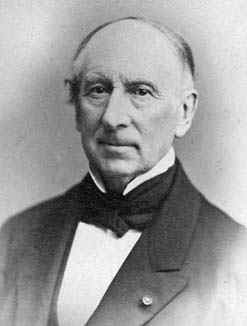
\includegraphics[height=25mm]{../image/Cauchy.jpeg}
		\hspace{2cm}
		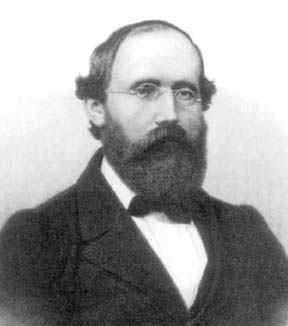
\includegraphics[height=25mm]{../image/Riemann.jpeg}
	\end{center}
\end{frame}


\begin{frame}{柯西-黎曼方程的等价形式\noexer}
	\onslide<+->
	注意到 $x=\dfrac12z+\dfrac12\ov z,y=-\dfrac i2z+\dfrac i2\ov z$.
	\onslide<+->
	仿照着二元实函数偏导数在变量替换下的变换规则, 我们定义 $f$ 对 $z$ 和 $\ov z$ 的偏导数为
	\[\laeq{\displaystyle
		\pp fz=\pp xz\pp fx+\pp yz\pp fy
		=\frac12\pp fx-\frac i2\pp fy,\\
		\displaystyle
		\pp f{\ov z}=\pp x{\ov z}\pp fx+\pp y{\ov z}\pp fy
		=\frac12\pp fx+\frac i2\pp fy.
	}.
	\]
	\onslide<+->
	如果把 $z,\ov z$ 看成独立变量, 那么当 $f$ 在 $z$ 处可导时,
	$\diff f=f'\diff z$.
	当 $f$ 关于 $z,\ov z$ 可微时(即 $u,v$ 可微),
	\[\diff f=\pp fz\diff z+\pp f{\ov z}\diff\ov z.
	\]
	\onslide<+->
	所以 \alert{$f$ 在 $z$ 处可导当且仅当 $u,v$ 可微且 $\dpp f{\ov z}=0$, 此时 $f'(z)=\dpp fz$.}
\end{frame}


\begin{frame}{可导的充分性条件}
	\onslide<+->
	由于二元函数的偏导数均连续蕴含可微, 因此我们有:

	\onslide<+->
	\begin{theorem}
		\begin{itemize}
			\item 如果 $u_x,u_y,v_x,v_y$ 在 $z$ 处连续, 且满足C-R方程, 则 $f(z)$ 在 $z$ 可导.
			\item 如果 $u_x,u_y,v_x,v_y$ 在区域 $D$ 上处处连续, 且满足C-R方程, 则 $f(z)$ 在 $D$ 上可导(从而解析).
		\end{itemize}
	\end{theorem}
\end{frame}


\subsection{柯西-黎曼方程的应用}
\begin{frame}{典型例题: 利用C-R方程判断可导和解析}
	\onslide<+->
	\begin{example}
		函数 $f(z)=\ov z$ 在何处可导, 在何处解析?
	\end{example}

	\onslide<+->
	\begin{solution}
		由 $u=x,v=-y$ 可知
		\begin{align*}
			u_x&=1,&u_y&=0,\\
			v_x&=0,&v_y&=-1.
		\end{align*}
		\onslide<+->{%
			因为 $u_x=1\neq v_y=-1$, 所以该函数处处不可导, 处处不解析.
		}
	\end{solution}
	\onslide<+->
	也可由 $\dpp f{\ov z}=1\neq0$ 看出.
\end{frame}


\begin{frame}{典型例题: 利用C-R方程判断可导和解析}
	\onslide<+->
	\begin{example}
		函数 $f(z)=z\Re z$ 在何处可导, 在何处解析?
	\end{example}

	\onslide<+->
	\begin{solution}
		由 $f(z)=x^2+\iixy,u=x^2,v=xy$
		\onslide<+->{%
			可知
			\begin{align*}
				u_x&=2x,&u_y&=0,\\
				v_x&=y, &v_y&=x.
			\end{align*}
		}\onslide<+->{%
			由 $2x=x,0=-y$ 可知只有 $x=y=0,z=0$ 满足C-R方程.
		}\onslide<+->{%
			因此该函数只在 $0$ 可导, 处处不解析且
			\[f'(0)=u_x(0)+\ii v_x(0)=0.
	\]
		}
		\vspace{-\baselineskip}
	\end{solution}
	\onslide<+->
	也可由 $f=\dfrac12 z(z+\ov z), \dpp f{\ov z}=\dfrac12 z$ 看出, $f'(0)=\dpp fz\Big|_{z=0}=z|_{z=0}=0$.
\end{frame}


\begin{frame}{典型例题: 利用C-R方程判断可导和解析}
	\onslide<+->
	\begin{example}
		函数 $f(z)=\ee^x(\cos y+\ii\sin y)$ 在何处可导, 在何处解析?
	\end{example}

	\onslide<+->
	\begin{solution}
		由 $u=\ee^x\cos y,v=\ee^x\sin y$
		\onslide<+->{%
			可知
			\begin{align*}
			u_x&=\ee^x\cos y,&u_y&=-\ee^x\sin y,\\
			v_x&=\ee^x\sin y,&v_y&=\ee^x\cos y.
			\end{align*}
		}\onslide<+->{%
			因此该函数处处可导, 处处解析, 且
			\[f'(z)=u_x+\ii v_x=\ee^x(\cos y+\ii\sin y)=f(z).
	\]
		}
	\vspace{-\baselineskip}
	\end{solution}

	\onslide<+->
	实际上, 这个函数就是复变量的指数函数 $\ee^z$.
\end{frame}


\begin{frame}{典型例题: 利用C-R方程判断可导和解析}
	\onslide<+->
	\begin{exercise}
		函数\fillbraceframe{A}在 $z=0$ 处不可导.
		\begin{exchoice}(2)
			() $2x+3yi$
			() $2x^2+3y^2\ii$
			() $\ee^x\cos y+\ii \ee^x\sin y$
			() $x^2-xyi$
		\end{exchoice}
	\end{exercise}

	\onslide<+->
	\begin{answer}
		根据C-R方程可知对于A, $u_x(0)=2\neq v_y(0)=3$.
		\onslide<+->{对于BD, 各个偏导数在 $0$ 处取值都是 $0$.
		}\onslide<+->{C则是处处都可导.}
	\end{answer}
\end{frame}


\begin{frame}{例: 利用C-R方程判断可导和解析}
	\onslide<+->
	\begin{example}
		设函数 $f(z)=(x^2+axy+by^2)+\ii(cx^2+dxy+y^2)$ 在复平面内处处解析. 求实常数 $a,b,c,d$ 以及 $f'(z)$.
	\end{example}

	\onslide<+->
	\begin{solution}
		由于
		\vspace{-\baselineskip}
		\begin{align*}
			u_x&=2x+ay,&u_y=ax+2by,\\
			v_x&=2cx+dy,&v_y=dx+2y,
		\end{align*}
		\onslide<+->{因此
			\[2x+ay=dx+2y,\quad ax+2by=-(2cx+dy),\]}
		\vspace{-\baselineskip}
		\onslide<+->{
			\[a=d=2,\quad b=c=-1,\]}
		\vspace{-\baselineskip}
		\onslide<+->{
			\[f'(z)=u_x+\ii v_x=2x+2y+\ii(-2x+2y)=(2-2\ii)z.\]}
		\vspace{-\baselineskip}
	\end{solution}
\end{frame}


\begin{frame}[<*>]{例: 利用C-R方程证明解析函数结论}
	\onslide<+->
	\begin{example}
		如果 $f'(z)$ 在区域 $D$ 内处处为零, 则 $f(z)$ 在 $D$ 内是一常数.
	\end{example}

	\onslide<+->
	\begin{proof}
		由于 $f'(z)=u_x+\ii v_x=v_y-\ii u_y=0$,
		\onslide<+->{%
			因此 $u_x=v_x=u_y=v_y=0$, $u,v$ 均为常数,
		}\onslide<+->{%
			从而 $f(z)=u+\ii v$ 是常数.\qedhere
		}
	\end{proof}

	\onslide<+->
	类似地可以证明, 若 $f(z)$ 在 $D$ 内解析, 则下述条件均可推出 $f(z)$ 是常数:
	\onslide<+->
	\begin{figure}[hbpt]
		\begin{minipage}{0.48\textwidth}
			\begin{itemize}
				\item $f'(z)=0$,
				\item $|f(z)|$ 是一常数,
				\item $\arg{f(z)}$ 是一常数,
			\end{itemize}
		\end{minipage}
		\begin{minipage}{0.48\textwidth}
			\begin{itemize}
				\item $\Re{f(z)}$ 是一常数,
				\item $\Im{f(z)}$ 是一常数,
				\item $v=u^2$.
			\end{itemize}
		\end{minipage}
	\end{figure}
\end{frame}


\begin{frame}{例: 解析函数的保角性\noexer}
	\beqskip{3pt}
	\onslide<+->
	\begin{example}
		如果 $f(z)$ 解析且 $f'(z)$ 处处非零, 则曲线族 $u(x,y)=c_1$ 和曲线族 $v(x,y)=c_2$ 互相正交.
	\end{example}

	\onslide<+->
	\begin{proof}[indent]
		由于 $f'(z)=u_x-\ii u_y$, 因此 $u_x,u_y$ 不全为零.
		\onslide<+->{%
			对 $u(x,y)=c_1$ 使用隐函数求导法则得 $u_x\diff x+u_y\diff y=0$,
		}\onslide<+->{%
			从而 $(u_y,-u_x)$ 是该曲线在 $z$ 处的非零切向量.
		}

		\onslide<+->{%
			同理 $(v_y,-v_x)$ 是 $v(x,y)=c_2$ 在 $z$ 处的非零切向量.
		}\onslide<+->{%
			由于
			\[u_yv_y+u_xv_x=u_yu_x-u_xu_y=0,
	\]
		}\onslide<+->{%
			因此二者正交.\qedhere
		}
	\end{proof}

	\onslide<+->
	当 $f'(z_0)\neq 0$ 时, 
	\onslide<+->
	经过 $z_0$ 的两条曲线 $C_1,C_2$ 的夹角和它们的像 $f(C_1),f(C_2)$ 在 $f(z_0)$ 处的夹角总是相同的.
	\onslide<+->
	这种性质被称为\emph{保角性}.
	\onslide<+->
	这是因为 $\diff f=f'(z_0)\diff z$.
	\onslide<+->
	局部来看 $f$ 把 $z_0$ 附近的点以 $z_0$ 为中心放缩 $f'(z_0)$ 倍并逆时针旋转 $\arg{f'(z_0)}$.
	\onslide<+->
	由 $w$ 复平面上曲线族 $u=c_1,v=c_2$ 正交可知上述例题成立.
	\endgroup
\end{frame}


\begin{frame}{复变函数在实变函数导数的应用\noexer}
	\onslide<+->
	最后我们来看复数在求导中的一个应用.
	\onslide<+->
	\begin{example}
		设 $f(z)=\dfrac1{1+z^2}$, 则它在除 $z=\pm i$ 外处处解析.
		\onslide<+->{%
			当 $z=x$ 为实数时,
		}\onslide<+->{%
			\begin{align*}
			\Bigl(\dfrac1{1+x^2}\Bigr)^{(n)}&=f^{(n)}(x)=\frac i2\left[\frac1{x+\ii}-\frac1{x-\ii }\right]^{(n)}\\
			&\visible<+->{=\frac i2\cdot(-1)^n n!\left[\frac1{(x+\ii)^{n+1}}-\frac1{(x-\ii )^{n+1}}\right]}\\
			&\visible<+->{=(-1)^{n+1}n!\Im\frac1{(x+\ii)^{n+1}}}\\
			&\visible<+->{=\frac{(-1)^nn!\sin[(n+1)\arccot x]}{(x^2+1)^{\frac{n+1}2}}.}
			\end{align*}}
			\vspace{-\baselineskip}
	\end{example}
	\onslide<+->
	任意有理函数的高阶导数均可按此法计算.
\end{frame}


\section{初等函数}

\subsection{指数函数}

\begin{frame}{指数函数}
	\onslide<+->
	我们将实变函数中的初等函数推广到复变函数.
	\onslide<+->
	多项式函数和有理函数的解析性质已经介绍过, 这里不再重复.
	\onslide<+->
	现在我们来定义指数函数.

	\onslide<+->
	指数函数有多种等价的定义方式:
	\begin{enumerate}
		\item $\exp z=\ee^x(\cos y+\ii\sin y)$ (欧拉恒等式);
		\item $\exp z=\liml_{n\to\infty}\Bigl(1+\dfrac zn\Bigr)^n$ (极限定义);
		\item $\exp z=1+z+\dfrac{z^2}{2!}+\dfrac{z^3}{3!}+\cdots
		=\liml_{n\to\infty}\sum\limits_{k=0}^n\dfrac{z^k}{k!}$ (级数定义);
		\item $\exp z$ 是唯一的一个处处解析的函数, 使得当 $z=x\in\BR$ 时, $\exp z=\ee^x$ ($\ee^x$ 的解析延拓).
	\end{enumerate}
\end{frame}


\begin{frame}{指数函数与欧拉恒等式}
	\onslide<+->
	有些人会从 $\ee^x,\cos x,\sin x$ 的泰勒展开
	\begin{align*}
		\ee^x&=1+x+\frac{x^2}{2!}+\frac{x^3}{3!}+\cdots\\
		\cos x&=1-\frac{x^2}{2!}+\frac{x^4}{4!}+\cdots\\
		\sin x&=x-\frac{x^3}{3!}+\frac{x^5}{5!}\cdots
	\end{align*}
	形式地带入得到欧拉恒等式 $\ee^{\ii x}=\cos x+\ii\sin x$.
	\onslide<+->
	事实上我们可以把它当做复指数函数的定义, 而不是欧拉恒等式的证明.
	\onslide<+->
	我们将在第四章说明\enumnum1、\enumnum3和\enumnum4是等价的.
\end{frame}



\begin{frame}{指数函数的定义}
	\onslide<+->
	我们来证明\enumnum1和\enumnum2等价.
	\onslide<+->
	\begin{align*}
		\lim_{n\to\infty}\Bigabs{1+\frac zn}^n
		&=\lim_{n\to\infty}\Bigl(1+\frac{2x}n+\frac{x^2+y^2}{n^2}\Bigr)^{\frac n2}\quad
		\visible<+->{(1^\infty\ \text{型不定式})}\\
		&\visible<+->{=\exp\left[\lim_{n\to\infty}\frac n2
		\Bigl(\frac{2x}n+\frac{x^2+y^2}{n^2}\Bigr)\right]=\ee^x.}
	\end{align*}
	\onslide<+->
	不妨设 $n>\abs{z}$, 这样 $1+\dfrac zn$ 落在右半平面,
	\onslide<+->
	\[
		\lim_{n\to\infty} n\arg{\Bigl(1+\frac zn\Bigr)}
		=\lim_{n\to\infty} n\arctan \frac y{n+x}
		\visible<+->{=\lim_{n\to\infty}\frac{ny}{n+x}=y.}
	\]
	\bigdel
	\onslide<+->
	故 $\exp z=\ee^x(\cos y+\ii\sin y)$.
\end{frame}


\begin{frame}{指数函数的性质}
	\onslide<+->
	\begin{definition*}[][指数函数]
	\[
		\exp z:=\ee^x(\cos y+\ii\sin y).
	\]
	\end{definition*}
	\onslide<+->
	为了方便, 我们也记 $\emphm{\ee^z=\exp z}$.
	\onslide<+->
	指数函数有如下性质:
	\begin{itemize}\bf
		\item $\exp z$ 处处解析, 且 $(\exp z)'=\exp z$.
		\item $\exp z\neq 0$.
		\item $\exp(z_1+z_2)=\exp z_1\cdot \exp z_2$.
		\item $\exp(z+2k\pi\ii)=\exp z$, 即 $\exp z$ 周期为 $2\pi\ii$.
		\item $\exp z_1=\exp z_2$ 当且仅当 $z_1=z_2+2k\pi\ii,k\in\BZ$.
		\item 指数函数将直线族 $\Re z=c$ 映为圆周族 $\abs{w}=\ee^c$, 将直线族 $\Im z=c$ 映为射线族 $\Arg w=c$.
	\end{itemize}
\end{frame}


\begin{frame}{指数函数的性质}
	\onslide<+->
	\begin{example}
		计算函数 $f(z)=\exp(z/6)$ 的周期.
	\end{example}

	\onslide<+->
	\begin{solution}
		设 $f(z_1)=f(z_2)$, 则 $\ee^{z_1/6}=\ee^{z_2/6}$.
		\onslide<+->{%
			因此存在 $k\in\BZ$ 使得
			\[
				\frac{z_1}6=\frac{z_2}6+2k\pi\ii,
			\]
		}\onslide<+->{%
			从而 $z_1-z_2=12k\pi\ii$.
		}\onslide<+->{%
			所以 $f(z)$ 的周期是 $12\pi\ii$.
		}
	\end{solution}

	\onslide<+->
	一般地, $\exp(az+b)$ 的周期是 $\dfrac{2\pi\ii}a$ (或写成 $-\dfrac{2\pi\ii}a$), $a\neq 0$.
\end{frame}


\subsection{对数函数}

\begin{frame}{对数函数}
	\onslide<+->
	对数函数 $\Ln z$ 定义为指数函数 $\exp z$ 的反函数.
	\onslide<+->
	为什么我们用大写的 $\Ln$ 呢? 
	\onslide<+->
	在复变函数中, 很多函数是多值函数.
	\onslide<+->
	为了便于研究, 我们会固定它的一个单值分支.
	\onslide<+->
	我们将多值的这个开头字母大写, 而对应的单值的则是开头字母小写.
	\onslide<+->
	例如 $\Arg z$ 和 $\arg z$.

	\onslide<+->
	设 $z\neq0,\ee^w=z=r\ee^{\ii\theta}=\ee^{\ln r+\ii\theta}$,
	\onslide<+->
	则
	\[w=\ln r+\ii\theta+2k\pi\ii,\quad k\in\BZ.
	\]
\end{frame}


\begin{frame}{对数函数及其主值}
	\onslide<+->
	\begin{definition*}{对数函数}
		\begin{enumerate}
			\item 定义\emph{对数函数}
			\[
				\Ln z=\ln\abs{z}+\ii\Arg z.
			\]
			它是一个多值函数.
			\item 定义\emph{对数函数主值}
			\[
				\ln z=\ln\abs{z}+\ii\arg z.
			\]
			\bigdel
		\end{enumerate}
	\end{definition*}

	\onslide<+->
	对于每一个整数 $k$, $\ln z+2k\pi\ii$ 都给出了 $\Ln z$ 的一个单值分支.
	\onslide<+->
	特别地, 当 $z=x>0$ 是正实数时, $\ln z$ 就是实变的对数函数.
\end{frame}


\begin{frame}{例题: 对数函数的计算}
	\onslide<+->
	\begin{example}
		求 $\Ln 2,\Ln(-1)$ 以及它们的主值.
	\end{example}

	\onslide<+->
	\begin{solution}
		\begin{enumerate}
			\item
			\[
				\Ln2=\ln2+2k\pi\ii, k\in\BZ,
			\]
			\onslide<+->{%
				主值为 $\ln 2$.
			}
			\item
			\[
				\Ln(-1)=\ln1+\ii\Arg(-1)=(2k+1)\pi\ii, k\in\BZ,
			\]
			\onslide<+->{%
				主值为 $\pi\ii$.
			}
		\end{enumerate}
	\end{solution}
\end{frame}


\begin{frame}{例题: 对数函数的计算}
	\beqskip{5pt}
	\onslide<+->
	\begin{example}
	求 $\Ln(-2+3\ii),\Ln(3-\sqrt3 i)$.
	\end{example}

	\onslide<+->
	\begin{solution}
		\begin{enumerate}
			\item
			\begin{align*}
				\Ln(-2+3\ii)&=\ln\abs{-2+3\ii}+\ii\Arg(-2+3\ii)\\
				&\visible<+->{=\frac 12\ln 13+\Bigl(-\arctan\frac 32+\pi+2k\pi\Bigr)\ii,\quad k\in\BZ.}
			\end{align*}
			\item
			\begin{align*}
				\Ln(3-\sqrt3\ii)&=\ln\abs{3+\sqrt 3\ii}+\ii\Arg(3-\sqrt 3\ii)\\
				&\visible<+->{=\ln 2\sqrt 3+\Bigl(-\frac\pi6+2k\pi\Bigr)\ii
				=\ln 2\sqrt 3+\Bigl(2k-\frac16\Bigr)\pi\ii,\quad k\in\BZ.}
			\end{align*}
		\end{enumerate}
		\vspace{-.5\baselineskip}
	\end{solution}
	\endgroup
\end{frame}


\begin{frame}{例题: 对数函数的计算}
	\onslide<+->
	\begin{example}
		解方程 $\ee^z-1-\sqrt 3\ii=0$.
	\end{example}

	\onslide<+->
	\begin{solution}
		由于 $1+\sqrt 3 i=2\ee^{\frac{\pi\ii}3}$,
		\onslide<+->{%
			因此
			\[
				z=\Ln(1+\sqrt 3\ii)=\ln 2+\Bigl(2k+\frac13\Bigr)\pi\ii,\quad k\in\BZ.
			\]
		}\bigdel
	\end{solution}

	\onslide<+->
	\begin{exercise}
		求 $\ln(-1-\sqrt3\ii)=$\fillblankframe[2cm][3mm]{$\ln 2-\dfrac{2\pi\ii}3$}.
	\end{exercise}
\end{frame}


\begin{frame}{对数函数的性质}
	\onslide<+->
	对数函数与其主值的关系是
	\[
		\emphn{\Ln z=\ln z+\Ln 1=\ln z+2k\pi\ii,\quad k\in\BZ}.
	\]

	\onslide<+->
	根据辐角以及辐角主值的相应等式, 我们有
	\[
		\Ln(z_1\cdot z_2)=\Ln z_1+\Ln z_2,\quad
		\Ln\frac{z_1}{z_2}=\Ln z_1-\Ln z_2,
	\]
	\[
		\Ln \sqrt[n]z=\dfrac1n\Ln z.
	\]
	\onslide<+->
	而当 $\abs{n}\ge 2$ 时, \alert{$\Ln z^n=n\Ln z$ 不成立}.
	\onslide<+->
	以上等式换成 $\ln z$ 均未必成立.
\end{frame}


\begin{frame}{对数函数的导数}
\beqskip{1pt}
	\onslide<+->
	设 $x$ 是正实数, 
	\onslide<+->
	则
	\[
		\ln (-x)=\ln x+\pi\ii,\quad
		\lim_{y\to0^-}\ln (-x+y\ii)=\ln x-\pi\ii,
	\]
	\onslide<+->
	因此 $\ln z$ 在负实轴和零处不连续.

	\onslide<+->
	而在其它地方 $-\pi<\arg z<\pi$, $\ln z$ 是 $\ee^z$ 在区域 $-\pi<\Im z<\pi$ 上的单值反函数, 
	\onslide<+->
	从而
	\alert{$(\ln z)'=\dfrac 1z$},
	\alert{$\ln z$ 在除负实轴和零处的区域解析}.

	\onslide<+->
	也可以通过C-R方程来得到 $\ln z$ 的解析性和导数: 当 $x>0$ 时,
	\[
		\ln z=\half \ln(x^2+y^2)+\ii\arctan \frac yx,
	\]
	\onslide<+->
	\[
		u_x=v_y=\frac x{x^2+y^2},\qquad v_x=-u_y=-\frac y{x^2+y^2},
	\]
	\[
		(\ln z)'=\frac{x-yi}{x^2+y^2}=\frac 1z.
	\]
	其它情形可取虚部为 $\arccot\dfrac xy$ 或 $\arccot\dfrac xy-\pi$ 类似证明.
\endgroup
\end{frame}


\subsection{幂函数}

\begin{frame}{幂函数的性质: $a$ 为整数时}
	\onslide<+->
	\begin{definition*}[][幂函数]
		\begin{enumerate}
			\item 设 $a\neq 0$, $z\neq 0$, 定义\emph{幂函数}
			\[
				w=z^a=\ee^{a\Ln z}
				=\exp\bigl[a\ln\abs{z}+\ii a(\arg z+2k\pi)\bigr],\quad k\in\BZ.
			\]
			\item \emph{幂函数的主值}为
			\[
				w=\ee^{a\ln z}=\exp\bigl(a\ln\abs{z}+\ii a\arg z\bigr).
			\]
		\end{enumerate}
		\bigdel
	\end{definition*}
	\onslide<+->
	根据 $a$ 的不同, 这个函数有着不同的性质.

	\onslide<+->
	当 $a$ 为整数时, 因为 $\ee^{2ak\pi\ii}=1$, 所以 $w=z^a$ 是单值的.
	\onslide<+->
	此时 $z^a$ 就是我们之前定义的乘幂.

	\onslide<+->
	当 $a$ 是非负整数时, $z^a$ 在复平面上解析;
	\onslide<+->
	当 $a$ 是负整数时, $z^a$ 在 $\BC-\{0\}$ 上解析.
\end{frame}


\begin{frame}{幂函数的性质: $a$ 为分数时}
	\onslide<+->
	当 $a=\dfrac pq$ 为分数, $p,q$ 为互质的整数且 $q>1$ 时,
	\onslide<+->
	\[
		z^{\frac pq}=\abs{z}^{\frac pq}\exp\left[\frac{\ii p(\arg z+2k\pi)}q\right],\quad k=0,1,\dots,q-1
	\]
	具有 $q$ 个值.
	\onslide<+->
	去掉负实轴和 $0$ 之后, 它的主值 $w=\exp(a\ln z)$ 是处处解析的.
	\onslide<+->
	事实上它就是 $\sqrt[q]{z^p}=(\sqrt[q]z)^p$.
	\onslide<+->
	\begin{center}
		\begin{tikzpicture}[scale=.8]
			\coordinate [label=below left:{$0$}] (O) at (0,0);
			\coordinate [label=below:{$x$}] (X) at (2,0);
			\coordinate [label=left:{$y$}] (Y) at (0,2);
			\draw[cstaxis] (O)--(X);
			\draw[cstaxis] (0,-2)--(Y);
			\draw[draw=white,cstfille1] (O) circle (1.3);
			\draw[cstdash,main] (0,0)--(-2,0);
			\draw[cstdash,cstra,third] (1.7,.7)to [bend left] (4.5,.7);
			\draw (3,1.7) node[third] {$w=z^{2/9}$};
			\begin{scope}[xshift=5cm]
				\coordinate [label=below left:{$0$}] (O) at (0,0);
				\fill[cstfille2,pattern color=second] (O)--({1.4*cos(40)},{1.4*sin(40)}) arc (40:-40:1.4)--cycle;
				\draw[cstdash,second] ({1.4*cos(40)},{-1.4*sin(40)})--(0,0)--({1.4*cos(40)},{1.4*sin(40)});
				\coordinate [label=below left:{$0$}] (O) at (0,0);
				\coordinate [label=below:{$u$}] (X) at (2,0);
				\coordinate [label=left:{$v$}] (Y) at (0,2);
				\draw[cstaxis] (-2,0)--(X);
				\draw[cstaxis] (0,-2)--(Y);
			\end{scope}
		\end{tikzpicture}
	\end{center}
\end{frame}


\begin{frame}{幂函数的性质: $a$ 为其他情形}
\onslide<+->
	对于其它的 $a$, $z^a$ 具有无穷多个值.
	\onslide<+->
	这是因为此时当 $k\neq0$ 时, $2k\pi a \ii$ 不可能是 $2\pi\ii$ 的整数倍. 
	\onslide<+->
	从而不同的 $k$ 得到的是不同的值.
	\onslide<+->
	去掉负实轴和 $0$ 之后,
	\onslide<+->
	它的主值 $w=\exp(a\ln z)$ 也是处处解析的.
	\onslide<+->
	\begin{center}
		\arrayrulecolor{second}
		\begin{tabular}{cccc} \toprule
			$a$& $z^a$ 的值& $z^a$ 的解析区域\\ \midrule
			&&$n\ge0$ 时处处解析\\
			\multirow{-2}*{整数 $n$}&\multirow{-2}*{单值}&$n<0$ 时除零点外解析\\ \midrule
			分数 $p/q$&$q$ 值&除负实轴和零点外解析\\ \midrule
			无理数或虚数&无穷多值&除负实轴和零点外解析\\ \bottomrule
		\end{tabular}
	\end{center}
\end{frame}


\begin{frame}{典型例题: 幂函数的计算}
	\onslide<+->
	\begin{example}
		求 $1^{\sqrt 2}$ 和 $\ii^\ii$.
	\end{example}
	\onslide<+->
	\begin{solution}
		\[
			1^{\sqrt2}=\ee^{\sqrt2\Ln1}
			\visible<+->{=\ee^{\sqrt 2\cdot 2k\pi\ii}}
			\visible<+->{=\cos(2\sqrt 2k\pi)+\ii\sin(2\sqrt 2k\pi), k\in\BZ.}
		\]
		\onslide<+->{%
			\[
				\ii^\ii=\ee^{\ii\Ln \ii}
				\visible<+->{=\exp\left[\ii\cdot\Bigl(2k+\half\Bigr)\pi\ii\right]}
				\visible<+->{=\exp\Bigl(-2k\pi-\half\pi\Bigr), k\in\BZ.}
			\]
		}\bigdel
	\end{solution}
	\onslide<+->
	\begin{exercise}
		$3^\ii$ 的辐角主值是\fillblankframe{$\ln 3$}.
	\end{exercise}
\end{frame}


\begin{frame}{幂函数的性质}
	幂函数与其主值有如下关系:
	\onslide<+->
	\[
		\emphn{z^a=\ee^{a\ln z}\cdot 1^a
		=\ee^{a\ln z}\cdot \ee^{2ak\pi\ii},\quad k\in\BZ.}
	\]

	\onslide<+->
	对于幂函数的主值,
	\[
		\alertn{(z^a)'}=\Bigl(\ee^{a\ln z}\Bigr)'=\frac{a\ee^{a\ln z}}z=\alertn{az^{a-1}}.
	\]

	\onslide<+->
	一般而言, $z^a\cdot z^b=z^{a+b}$ 和 $(z^a)^b=z^{ab}$ 都是不成立的.

	\onslide<+->
	最后, 注意 $\ee^a$ 作为指数函数 $f(z)=\ee^z$ 在 $a$ 处的值和作为 $g(z)=z^a$ 在 $e$ 处的值是\alert{不同}的.
	\onslide<+->
	因为后者在 $a\not\in\BZ$ 时总是多值的.
	\onslide<+->
	前者实际上是后者的主值.
	\onslide<+->
	为避免混淆, 以后我们总\alert{默认 $\ee^a$ 表示指数函数 $\exp a$}.
\end{frame}


\subsection{三角函数和反三角函数}

\begin{frame}{三角函数的定义}
	\onslide<+->
	我们知道
	\[
		\cos x=\frac{\ee^{\ii x}+\ee^{-\ii x}}2,\quad
		\sin x=\frac{\ee^{\ii x}-\ee^{-\ii x}}{2\ii}
	\]
	对于任意实数 $x$ 成立,
	\onslide<+->
	我们将其推广到复数情形.
	\onslide<+->
	\begin{definition*}[][余弦和正弦函数]
		\[
			\cos z=\frac{\ee^{\ii z}+\ee^{-\ii z}}2,\quad
			\sin z=\frac{\ee^{\ii z}-\ee^{-\ii z}}{2\ii}.
		\]
	\end{definition*}
	\onslide<+->
	那么欧拉恒等式 \emph{$\ee^{\ii z}=\cos z+\ii\sin z$ 对任意复数 $z$ 均成立}.
\end{frame}


\begin{frame}{三角函数的性质}
	\onslide<+->
	不难得到
	\[
		\cos(\ii y)=\dfrac{\ee^y+\ee^{-y}}2,\qquad
		\visible<+->{\sin(\ii y)=\ii\dfrac{\ee^y-\ee^{-y}}2.}
	\]
	\onslide<+->
	当 $y\to\infty$ 时, $\cos(\ii y)$ 和 $\sin(\ii y)$ 都 $\to\infty$.
	\onslide<+->
	因此 \alert{$\sin z$ 和 $\cos z$ 并不有界}. 
	\onslide<+->
	这和实变情形完全不同.

	\onslide<+->
	容易看出 $\cos z$ 和 $\sin z$ 的零点都是实数.
	\onslide<+->
	于是我们可类似定义其它三角函数
	\begin{align*}
		\alertn{\tan z}&
		\alertn{=\frac{\sin z}{\cos z},z\neq\Bigl(k+\half\Bigr)\pi,}&
		\alertn{\cot z}&
		\alertn{=\frac{\cos z}{\sin z},z\neq k\pi,}\\
		\alertn{\sec z}&
		\alertn{=\frac{1}{\cos z},z\neq\Bigl(k+\half\Bigr)\pi,}&
		\alertn{\csc z}&
		\alertn{=\frac{1}{\sin z},z\neq k\pi.}
	\end{align*}
\end{frame}


\begin{frame}{三角函数的性质}
	\onslide<+->
	这些三角函数的奇偶性, 周期性和导数与实变情形类似,
	\[
		\alertn{(\cos z)'=-\sin z,\quad
		(\sin z)'=\cos z,}
	\]
	\onslide<+->
	且在定义域范围内是处处解析的.

	\onslide<+->
	三角函数的各种恒等式在复数情形也仍然成立,
	\onslide<+->
	例如
	\begin{itemize}
		\item $\cos(z_1\pm z_2)=\cos z_1 \cos z_2\mp \sin z_1 \sin z_2$,
		\item $\sin(z_1\pm z_2)=\sin z_1 \cos z_2\pm\cos z_1 \sin z_2$,
		\item $\sin^2z+\cos^2z=1$.
	\end{itemize}
\end{frame}


\begin{frame}{双曲函数}
	\onslide<+->
	类似的, 我们可以定义双曲函数:
	\onslide<+->
	\[
		\alertn{\ch z=\frac{\ee^z+\ee^{-z}}2=\cos \ii z,}
	\]
	\onslide<+->
	\[
		\alertn{\sh z=\frac{\ee^z-\ee^{-z}}2=-\ii \sin \ii z,}
	\]
	\onslide<+->
	\[
		\alertn{\tanh z=\frac{\ee^z-\ee^{-z}}{\ee^z+\ee^{-z}}
		=-\ii \tan \ii z,\quad z\neq \Bigl(k+\half\Bigr)\pi\ii.}
	\]
	\onslide<+->
	它们的奇偶性和导数与实变情形类似, 在定义域范围内是处处解析的.

	\onslide<+->
	$\ch z,\sh z$ 的周期是 $2\pi\ii$, $\tanh z$ 的周期是 $\pi\ii$.
\end{frame}


\begin{frame}{反三角函数和反双曲函数}
	\onslide<+->
	设 $z=\cos w=\dfrac{\ee^{\ii w}+\ee^{-\ii w}}2$,
	\onslide<+->
	则
	\[
		\ee^{2\ii w}-2z\ee^{\ii w}+1=0,\quad
		\visible<+->{\ee^{\ii w}=z+\sqrt{z^2-1}\ \text{(双值)}.}
	\]
	\onslide<+->
	因此\emph{反余弦函数}为
	\[
		w=\Arccos z=-\ii \Ln(z+\sqrt{z^2-1}).
	\]
	\onslide<+->
	显然它是多值的.
	\onslide<+->
	同理, 我们有:
	\begin{itemize}
		\item \emph{反正弦函数} $\Arcsin z=-\ii \Ln(\ii z+\sqrt{1-z^2})$;
		\item \emph{反正切函数} $\Arctan z=-\dfrac \ii2\Ln\dfrac{1+\ii z}{1-\ii z}, z\neq \pm \ii$;
		\item \emph{反双曲余弦函数} $\Arch z=\Ln(z+\sqrt{z^2-1})$;
		\item \emph{反双曲正弦函数} $\Arsh z=\Ln(z+\sqrt{z^2+1})$;
		\item \emph{反双曲正切函数} $\Arth z=\dfrac12\Ln\dfrac{1+z}{1-z}, z\neq \pm1$.
	\end{itemize}
\end{frame}


\begin{frame}{例题: 解三角函数方程}
	\onslide<+->
	\begin{example}
		解方程 $\sin z=2$.
	\end{example}
	\onslide<+->
	\begin{solution}
	由于 $\sin z=\dfrac{\ee^{\ii z}-\ee^{-\ii z}}{2\ii}=2$,
	\onslide<+->{%
		我们有
		\[
			\ee^{2\ii z}-4\ii\ee^{\ii z}-1=0.
		\]
	}\onslide<+->{%
		于是 $\ee^{\ii z}=(2\pm\sqrt 3)\ii$,
	}\onslide<+->{%
		\[
			z=-\ii \Ln[(2\pm\sqrt 3)\ii]=\Bigl(2k+\half\Bigr)\pi\pm \ii\ln(2+\sqrt3),\quad k\in\BZ.
		\]
	}\bigdel
	\end{solution}
\end{frame}

\begin{frame}{例题: 解三角函数方程}
	\onslide<+->
	\begin{solution}[][另解]
	由 $\sin z=2$ 可知
	\[
		\cos z=\sqrt{1-\sin^2 z}=\pm\sqrt 3\ii.
	\]
	\onslide<+->{%
		于是 $\ee^{\ii z}=\cos z+\ii\sin z=(2\pm\sqrt 3)\ii$,
	}\onslide<+->{%
		\[
			z=-\ii \Ln[(2\pm\sqrt 3)\ii]=\Bigl(2k+\half\Bigr)\pi\pm \ii\ln(2+\sqrt3),\quad k\in\BZ.
		\]
	}\bigdel
	\end{solution}
	\onslide<+->
	对于任意 $z$, 总存在 $\theta$ 使得
	\begin{align*}
		\Arcsin z&=(2k+\half)\pi\pm \theta,\\
		\Arccos z&=2k\pi\pm \theta,\\
		\Arctan z&=k\pi+\theta,\quad (z\ne\pm\ii).
	\end{align*}
\end{frame}


\subsection{在有理函数的应用}


\begin{frame}{有理函数分拆}
	\onslide<+->
	称分子次数小于分母次数的有理函数为\emph{真分式}.
	\onslide<+->
	任何一个有理函数 $f(z)$ 都可以通过带余除法分解为一个多项式 $g(z)$ 和一个真分式之和.

	\onslide<+->
	若这个有理函数分母的零点均能求出, 则这个真分式又可以分拆为部分分式之和, 其中\emph{部分分式}是指形如 $\dfrac{a}{(x-b)^k}$ 的真分式.
	\onslide<+->
	我们来介绍求这种分拆的一种方法.
\end{frame}


\begin{frame}{例题: 有理函数分拆}
	\beqskip{2pt}
	\onslide<+->
	\begin{example}[near]
		将 $f(z)=\dfrac{1}{(z-1)(z-2)^2}$ 展开成部分分式之和.
	\end{example}
	\onslide<+->
	\begin{solution}[near]
		设 $f(z)=\dfrac{a}{z-1}+\dfrac{b}{z-2}+\dfrac{c}{(z-2)^2}$,
		\onslide<+->{%
			则
			\begin{align*}
				a&=\lim_{z\ra1} (z-1)f(z)
					=\lim_{z\ra1} \frac{1}{(z-2)^2}
					=1,\\
				\onslide<+->{b}&\onslide<.->{=\lim_{z\ra2} \bigl((z-2)^2f(z)\bigr)'
					=\lim_{z\ra2} \Bigl(\frac{1}{z-1}\Bigr)'
					=-1,}\\
				\onslide<+->{c}&\onslide<.->{=\lim_{z\ra2} (z-2)^2f(z)
					=\lim_{z\ra2} \frac{1}{z-1}=1.}
			\end{align*}
		}\onslide<+->{%
			因此
			\[
				f(z)=\frac{1}{z-1}-\frac{1}{z-2}+\frac{1}{(z-2)^2}.
			\]
		}\bigdel
	\end{solution}
	\endgroup
\end{frame}


\begin{frame}{有理函数的导数\noexer}
	\onslide<+->
	得到这种分拆之后, 我们可以求出该有理函数的任意阶导数.
	\onslide<+->
	\begin{example}[nearnext]
		计算 $f(x)=\dfrac1{1+x^2}$ 的 $n$ 阶导数.
	\end{example}
	\onslide<+->
	\begin{solution}[nearprev]
		设
		\[
			f(z)
			=\frac1{1+z^2}
			=\frac \ii2\biggl(\frac1{z+\ii}-\frac1{z-\ii}\biggr),
		\]
		\onslide<+->{%
			则它在除 $z=\pm \ii$ 外处处解析,
		}\onslide<+->{%
			且
			\begin{align*}
				f^{(n)}(z)&
				=\frac \ii2\biggl(\frac1{z+\ii}-\frac1{z-\ii}\biggr)^{(n)}
				\onslide<+->{=\frac \ii2\cdot(-1)^n n!\biggl(\frac1{(z+\ii)^{n+1}}-\frac1{(z-\ii)^{n+1}}\biggr)}\\&
				\onslide<+->{=(-1)^{n+1}n!\Im{(z+\ii)^{-n-1}}.}
			\end{align*}
		}\bigdel
	\end{solution}
\end{frame}
	
	
\begin{frame}{有理函数的导数}
	\onslide<+->
	\begin{solution}[][]%
		当 $z=x$ 为实数时,
		\[
			\abs{x+\ii}=\sqrt{x^2+1},\qquad
			\arg(x+\ii)=\arccot x,
		\]
		\onslide<+->{%
			于是
			\[
				\frac1{(z\pm\ii)^{n+1}}=(x^2+1)^{-\frac{n+1}2}\ee^{\pm\ii (n+1)\arccot x}.
			\]
		}\onslide<+->{%
			因此
			\[
				\biggl(\frac1{1+x^2}\biggr)^{(n)}
				=(-1)^nn!(x^2+1)^{-\frac{n+1}2}\sin\bigl((n+1)\arccot x\bigr).
			\]
		}
	\end{solution}
\end{frame}


\begin{frame}{有理函数的不定积分\noexer}
	\onslide<+->
	我们还可以利用复对数函数来计算实有理函数的不定积分.
	\onslide<+->
	\begin{example}[nearnext]
		计算 $\dint \frac1{x^3-1}\d x$.
	\end{example}
	\onslide<+->
	\begin{solution}[nearprev]
		设 $\zeta=\ee^{\frac{2\cpi\ii}3}=\dfrac{-1+\sqrt3\ii}2$, 
		\onslide<+->{%
			那么我们有分拆
			\[
				f(x)
				=\frac1{x^3-1}
				=\frac13\Bigl(\frac{1}{x-1}+\frac{\zeta}{x-\zeta}+\frac{\zeta^2}{x-\zeta^2}\Bigr),
			\]
		}\onslide<+->{%
			设
			\[
				g(z)=\frac13\bigl(
					\ln(z-1)+\zeta\ln(z-\zeta)+\zeta^2\ln(z-\zeta^2)
				\bigr).
			\]
		}\bigdel
	\end{solution}
\end{frame}
	
	
\begin{frame}{有理函数的不定积分\noexer}
	\beqskip{5pt}
	\onslide<+->
	\begin{solution}[][]%
		$g(z)$ 在复平面去掉三条射线 $x+\zeta^k,x\le 0$ 内的导数为 $f(z)$.
		\onslide<+->{%
			当 $z=x>1$ 时, 
			\begin{align*}
				&3g(z)-\ln(x-1)=2\Re\bigl(\zeta\ln(x-\zeta)\bigr)
				=2\Re\biggl(\frac{-1+\sqrt3\ii}2\ln\Bigl(x-\frac{-1+\sqrt3\ii}2\Bigr)\biggr)\\
				={}&2\Re\biggl(
					\frac{-1+\sqrt3\ii}2
						\Bigl(\ln\sqrt{x^2+x+1}-\ii\arccot\frac{2x+1}{\sqrt3}\Bigr)
					\biggr)\\
				={}&\ln\sqrt{x^2+x+1}+\sqrt 3\arccot\frac{2x+1}{\sqrt3}.
			\end{align*}
		}\onslide<+->{%
			于是我们得到当 $x>1$ 时,
			\[
				g(x)=\frac13\ln\abs{x-1}-\frac16\ln(x^2+x+1)
					+\frac{\sqrt3}3\arccot\frac{2x+1}{\sqrt3}.
			\]
		}\onslide<+->{%
			可以看出对于实数 $x<1$, 上式的导数也等于 $f(x)$, 从而 $f(x)$ 的不定积分为 $g(x)+C$, $C\in\BR$.
		}
	\end{solution}
	\endgroup
\end{frame}

\part{复变函数的积分}
\section{复变函数积分的概念}

\subsection{复变函数积分的定义}

\begin{frame}{有向曲线}
	\onslide<+->
	设 $C$ 是平面上一条光滑或逐段光滑的连续曲线,
	\onslide<+->
	也就是说它的参数方程 $z=z(t),a\le t\le b$ 除去有限个点之外都有非零导数.
	\onslide<+->
	这里 $z'(t)=x'(t)+\ii y'(t)$.

	\onslide<+->
	固定它的一个方向, 称为\emph{正方向}, 则我们得到一条\emph{有向曲线}.
	\onslide<+->
	和这条曲线方向相反的记作 $C^-$, 它的方向被称为该曲线\emph{负方向}.

	\onslide<+->
	对于闭路, 它的\alert{正方向总是指逆时针方向}, 负方向总是指顺时针方向.
	\onslide<+->
	以后我们不加说明的话\alert{默认是正方向}.

	\onslide<2->
	\begin{center}
		\begin{tikzpicture}
			\draw[cstaxis](-3.5,0)--(3.5,0);
			\draw[cstaxis](0,-0.5)--(0,2.5);
			\begin{scope}[xshift=18mm,yshift=11mm,second,cstdot,cstcurve,smooth]
				\coordinate [label=left:{$A=z(a)$}] (A) at ({1.3*cos(-35)}, {1.3*sin(-35)});
				\coordinate [label=below:{$B=z(b)$}] (B) at ({1.3*cos(125)}, {1.3*sin(125)});
				\draw[main,domain=-35:125] plot ({1.3*cos(\x)}, {1.3*sin(\x)});
				\draw[main,domain=40:45,cstwra,visible on=<4->] plot ({1.3*cos(\x)}, {1.3*sin(\x)});
				\fill (A) circle;
				\fill (B) circle;
			\end{scope}
			\begin{scope}[xshift=-18mm,yshift=13mm,cstcurve,main,smooth,cstwla,visible on=<6->]
				\draw[domain=-65:30] plot ({-cos(\x)}, {.8*sin(\x)});
				\draw[domain=25:120] plot ({-cos(\x)}, {.8*sin(\x)});
				\draw[domain=115:210] plot ({-cos(\x)}, {.8*sin(\x)});
				\draw[domain=205:300] plot ({-cos(\x)}, {.8*sin(\x)});
			\end{scope}
		\end{tikzpicture}
	\end{center}
\end{frame}


\begin{frame}{复变函数积分: 线积分定义}
	\onslide<+->
	所谓的复变函数积分, 本质上仍然是第二类曲线积分.
	\onslide<+->
	设复变函数
	\[
		w=f(z)=u(x,y)+\ii v(x,y)
	\]
	定义在区域 $D$ 内, 有向曲线 $C$ 包含在 $D$ 中.
	\onslide<+->
	形式地展开
	\[
		f(z)\d z=(u+\ii v)(\d x+\ii\d y)=(u\d x-v\d y)+\ii(u\d y+v\d x).
	\]
	\bigdel
	\onslide<+->
	\begin{definition}
		若下述右侧两个线积分均存在, 则定义
	\[
			\int_C f(z)\d z=\int_C(u\d x-v\d y)+\ii\int_C(v\d x+u\d y)
	\]
		为 \emph{$f(z)$ 沿曲线 $C$ 的积分}.
	\end{definition}
\end{frame}


\begin{frame}{复变函数积分: 黎曼积分定义}
	\onslide<+->
	当然, 我们也可以像线积分那样通过分割来定义.
	\onslide<+->
	在曲线 $C$ 上依次选择分点 $z_0=A,z_1,\dots,z_{n-1},z_n=B$.
	\onslide<+->
	然后在每一段弧上任取 $\zeta_k\in\warc{z_{k-1}z_k}$ 并作和式
	\[
		S_n=\sum_{k=1}^n f(\zeta_k)\delt z_k,\quad \delt z_k=z_k-z_{k-1}.
	\]
	\onslide<+->
	然后称 $n\to\infty$, 分割的最大弧长 $\ra 0$ 时 $S_n$ 的极限为复变函数积分.
	\onslide<+->
	这二者是等价的.

	\onslide<2->
	\begin{center}
		\begin{tikzpicture}
			\draw[cstcurve,third,smooth,domain=0:360] plot ({0.015*\x},{0.6*sin(\x)});
			\draw[cstcurve,third,smooth,domain=195:200,cstra] plot ({0.015*\x},{0.6*sin(\x)});
			\begin{scope}[cstdot,third]
				\coordinate [label=left:{$A$}] (A);
				\coordinate [label=right:{$B$}] (B) at ({0.015*360},0) circle;
				\fill (A) circle;
				\fill (B) circle;
			\end{scope}
			\begin{scope}[cstdot,main,visible on=<2->]
				\coordinate [label=above:{$z_1$}] (z1) at ({0.015*64},{0.6*sin(64)});
				\coordinate [label=above:{$z_2$}] (z2) at ({0.015*128},{0.6*sin(128)});
				\coordinate [label=above:{$z_{n-2}$}] (zn2) at ({0.015*232},{0.6*sin(232)});
				\coordinate [label=above:{$z_{n-1}$}] (zn1) at ({0.015*296},{0.6*sin(296)});
				\coordinate [label=above:{$\ddots$}] (ddots) at ($(z1)!.5!(zn2)$);
				\fill (z1) circle;
				\fill (z2) circle;
				\fill (zn2) circle;
				\fill (zn1) circle;
			\end{scope}
			\begin{scope}[cstdot,second,visible on=<3->]
				\coordinate [label=below:{$\zeta_1$}] (zeta1) at ({0.015*32},{0.6*sin(32)});
				\coordinate [label=below:{$\zeta_2$}] (zeta2) at ({0.015*96},{0.6*sin(96)}) circle;
				\coordinate [label=below:{$\zeta_3$}] (zeta3) at ({0.015*160},{0.6*sin(160)}) circle;
				\coordinate [label=below:{$\zeta_{n-1}$}] (zetan1) at ({0.015*264},{0.6*sin(264)}) circle;
				\coordinate [label=below:{$\zeta_n$}] (zetan) at ({0.015*328},{0.6*sin(328)}) circle;
				\fill (zeta1) circle;
				\fill (zeta2) circle;
				\fill (zeta3) circle;
				\fill (zetan1) circle;
				\fill (zetan) circle;
			\end{scope}
		\end{tikzpicture}
	\end{center}
\end{frame}


\begin{frame}{复变函数积分的存在性}
	\onslide<+->
	若 $C$ 是闭路, 则该积分记为 \alert{$\doint_Cf(z)\d z$}.
	\onslide<+->
	此时该积分不依赖端点的选取.

	\onslide<+->
	若 $C$ 是实轴上的区间 $[a,b]$ 且 $f(z)=u(x)$, 
	\onslide<+->
	则
	\[
		\int_Cf(z)\d z=\int_a^bf(z)\d z=\int_a^b u(x)\d x
	\]
	就是黎曼积分.

	\onslide<+->
	根据线积分的存在性条件可知:
	\onslide<+->
	\begin{theorem}
		若 $f(z)$ 在 $D$ 内连续, $C$ 是光滑曲线, 则 $\dint_Cf(z)\d z$ 总存在.
	\end{theorem}
\end{frame}


\subsection{参变量法计算复变函数积分}

\begin{frame}{复变函数积分的计算法}
	\onslide<+->
	线积分中诸如变量替换等技巧可以照搬过来使用.
	\onslide<+->
	设
	\[
		C:z(t)=x(t)+\ii y(t),\quad a\le t\le b
	\]
	是一条光滑有向曲线, 且正方向为 $t$ 增加的方向,
	\onslide<+->
	则 $\d z=z'(t)\d t=\bigl(x'(t)+y'(t)\bigr)\d t$.
	\onslide<+->
	\begin{theorem*}[][积分计算方法I: 参变量法]
		\[
			\int_Cf(z)\d z=\int_a^b f\bigl(z(t)\bigr)z'(t)\d t.
		\]
	\end{theorem*}
	\onslide<+->
	若 $C$ 的正方向是从 $z(b)$ 到 $z(a)$, 则需要交换右侧积分的上下限.

	\onslide<+->
	若 $C$ 是逐段光滑的, 则相应的积分就是各段的积分之和.
	\onslide<+->
	以后我们\alert{只考虑逐段光滑曲线上的连续函数的积分}.
\end{frame}


\begin{frame}{典型例题: 计算复变函数沿曲线的积分}
	\onslide<+->
	\begin{example}[nearnext]
		求 $\dint_Cz\d z$, 其中 $C$ 是从原点到点 $3+4\ii$ 的直线段.
	\end{example}
	\onslide<+->
	\begin{solution}[nearprev,sidepic,righthand width=113pt]
		由于 $z=(3+4\ii)t,0\le t\le 1$,
		\onslide<+->{%
		因此
		\begin{align*}
			\int_Cz\d z&
			=\int_0^1(3+4\ii)t\cdot(3+4\ii)\d t
			\onslide<+->{=(3+4\ii)^2\int_0^1t\d t}\\&
			\onslide<+->{=\half (3+4\ii)^2=-\frac72+12\ii.}
		\end{align*}
		}\bigdel
		\tcblower
		\begin{tikzpicture}
			\coordinate (O) at (0,0);
			\draw[cstaxis](O)--(3,0);
			\draw[cstaxis](O)--(0,2.5);
			\coordinate (A) at (1.5,2);
			\draw[cstcurve,main,cstwra](O)--(A);
			\draw (A) node[below right,main,align=center] {$z=(3+4\ii)t$\\$0\le t\le 1$};
		\end{tikzpicture}
	\end{solution}
\end{frame}


\begin{frame}{典型例题: 计算复变函数沿曲线的积分}
	\onslide<+->
	\begin{example}[nearnext]
		求 $\dint_Cz\d z$, 其中 $C$ 是抛物线 $y=\dfrac49x^2$ 上从原点到点 $3+4\ii$ 的曲线段.
	\end{example}
	\onslide<+->
	\begin{solution}[nearprev,sidepic,righthand width=110pt]
		由于 $z=t+\dfrac49\ii t^2,0\le t\le 3$,
		\onslide<+->{%
			因此
			\begin{align*}
				\int_Cz\d z&=\int_0^3\biggl(t+\frac{4}9\ii t^2\biggr)\cdot\biggl(1+\frac89\ii t\biggr)\d t\\
				&\onslide<+->{=\int_0^3\biggl(t+\frac43\ii t^2-\frac{32}{81}t^3\biggr)\d t}\\
				&\onslide<+->{=\biggl(\half t^2+\frac49\ii t^3-\frac8{81}t^4\biggr)\Big|_0^3}
				\onslide<+->{=-\frac72+12\ii.}
			\end{align*}
		}\bigdel
		\tcblower
		\begin{tikzpicture}
			\draw[cstaxis](O)--(3,0);
			\draw[cstaxis](O)--(0,2.5);
			\draw[cstcurve,main,domain=0:1.5,cstwra] plot({\x},{8*\x*\x/9});
			\draw (A) node[right,main,align=center] {$z=t+\dfrac49\ii t^2$\\[1mm]$0\le t\le 3$};
		\end{tikzpicture}
	\end{solution}
\end{frame}


\begin{frame}{典型例题: 计算复变函数沿曲线的积分}
	\onslide<+->
	\begin{example}[nearnext]
		求 $\dint_C\Re z\d z$, 其中 $C$ 是从原点到点 $1+\ii$ 的直线段.
	\end{example}
	\onslide<+->
	\begin{solution}[nearprev,sidepic,righthand width=122pt]
		由于 $z=(1+\ii)t,0\le t\le 1$,
		\onslide<+->{%
			因此 $\Re z=t$,
		}\onslide<+->{%
			\begin{align*}
				\int_C\Re z\d z&
				=\int_0^1t\cdot(1+\ii)\d t\\&
				\onslide<+->{=(1+\ii)\int_0^1t\d t}
				\onslide<+->{=\frac{1+\ii}2.}
			\end{align*}
		}\bigdel
		\tcblower
		\begin{tikzpicture}
			\draw[cstaxis](O)--(3,0);
			\draw[cstaxis](O)--(0,2);
			\coordinate (B) at (2,2);
			\draw[cstcurve,main,cstwra](O)--(B);
			\draw (B) node[below right,main,align=center] {$z=(1+\ii)t$\\$0\le t\le 1$};
		\end{tikzpicture}
	\end{solution}
\end{frame}


\begin{frame}{典型例题: 计算复变函数沿曲线的积分}
	\onslide<+->
	\begin{example}[nearnext]
		求 $\dint_C\Re z\d z$, 其中 $C$ 是从原点到点 $\ii$ 再到 $1+\ii$ 的折线段.
	\end{example}
	\onslide<+->
	\begin{solution}[nearprev,sidepic,righthand width=146pt]
		第一段 $z=\ii t$, $0\le t\le 1$, $\Re z=0$,
		\onslide<+->{%
			第二段 $z=t+\ii$, $0\le t\le 1$, $\Re z=t$.
		}\onslide<+->{%
			因此
			\[
				\int_C\Re z\d z=\int_0^1 t\d t=\frac12.
			\]
		}\bigdel
		\tcblower
		\begin{tikzpicture}
			\draw[cstaxis](O)--(2.5,0);
			\draw[cstaxis](O)--(0,2);
			\coordinate (C) at (0,1.5);
			\coordinate (D) at (1.5,1.5);
			\draw[cstcurve,main,cstwra](O)--(C);
			\draw[cstcurve,second,cstwra,visible on=<3->](C)--(D);
			\draw
				(C) node[below left,align=center,main] {$z=\ii t$\\$0\le t\le 1$}
				(D) node[right,align=center,second,visible on=<3->] {$z=t+\ii$\\$0\le t\le 1$};
		\end{tikzpicture}
	\end{solution}
\end{frame}


\begin{frame}{典型例题: 计算复变函数沿曲线的积分}
	\onslide<+->
	可以看出, 即便起点和终点相同, 沿不同路径 $f(z)=\Re z$ 的积分也可能不同.
	\onslide<+->
	而 $f(z)=z$ 的积分则只和起点和终点位置有关, 与路径无关.
	\onslide<+->
	原因在于 $f(z)=z$ 是处处解析的, 我们会在下一节解释为何如此.

	\onslide<+->
	\begin{exercise}[sidepic,righthand width=96pt]
		求 $\dint_C\Im z\d z=$\fillblankframe[3cm][2mm]{$-\dfrac12+\dfrac\ii2$}, 其中 $C$ 是从原点沿 $y=x$ 到点 $1+\ii$ 再到 $\ii$ 的折线段.
		\tcblower
		\begin{center}
			\begin{tikzpicture}
				\draw[cstaxis](O)--(2,0);
				\draw[cstaxis](O)--(0,2);
				\draw[cstcurve,cstwra,main](O)--(D);
				\draw[cstcurve,cstwra,second](D)--(C);
			\end{tikzpicture}
		\end{center}
	\end{exercise}
\end{frame}


\begin{frame}{例题: 计算复变函数沿圆周的积分}
	\onslide<+->
	\begin{example}[nearnext]
		求 $\doint_{\abs{z-z_0}=r}\frac{\d z}{(z-z_0)^{n+1}}$, 其中 $n$ 为整数.
	\end{example}
	\onslide<+->
	\begin{solution}[nearprev]
		$C: \abs{z-z_0}=r$ 的参数方程为 $z=z_0+r\ee^{\ii\theta},0\le \theta\le 2\pi$.
		\onslide<+->{%
			于是 $\d z=\ii r\ee^{\ii\theta}\d \theta$.
		}\onslide<+->{%
			\begin{align*}
				\alertn{\oint_C\frac{\d z}{(z-z_0)^{n+1}}}
				&=\int_0^{2\pi}\ii(r\ee^{\ii\theta})^{-n}\d\theta
				\onslide<+->{=\ii r^{-n}\int_0^{2\pi}\ee^{-\ii n\theta}\d\theta}\\
				&\onslide<+->{=\ii r^{-n}\int_0^{2\pi}\bigl(\cos(n\theta)+\ii\sin(n\theta)\bigr)\d\theta}
				\onslide<+->{=\begin{cases}
					\alertn{2\pi\ii,}&\alertn{\text{\alert{若}}\ n=0;}\\
					\alertn{0,}&\alertn{\text{\alert{若}}\ n\neq0.}
				\end{cases}}
			\end{align*}
		}
	\end{solution}
	\onslide<+->
	这个积分以后经常用到, 它的特点是积分值与圆周的圆心和半径都无关.
\end{frame}


\begin{frame}{积分的性质}
	\onslide<+->
	\begin{theorem}[][线性性质]
		\begin{enumerate}
			\item $\dint_Cf(z)\d z=-\dint_{C^-}f(z)\d z$.
			\item $\dint_Ckf(z)\d z=k\dint_Cf(z)\d z$.
			\item $\dint_C[f(z)\pm g(z)]\d z
			=\dint_Cf(z)\d z\pm\dint_Cg(z)\d z$.
		\end{enumerate}
	\end{theorem}
\end{frame}


\subsection{长大不等式和大小圆弧引理}


\begin{frame}{长大不等式\noexer}
	\onslide<+->
	\begin{theorem*}[nearnext][长大不等式]
		设有向曲线 $C$ 的长度为 $L$, $f(z)$ 在 $C$ 上满足 $\abs{f(z)}\le M$, 则
		\[
			\biggabs{\int_C f(z)\d z}\le\int_C \abs{f(z)}\d s\le ML.
		\]
	\end{theorem*}
	\onslide<+->
	\begin{proof}[nearprev]
		对
			$\displaystyle
				\biggabs{\sum_{k=1}^n f(\zeta_k)\delt z_k}
				\le\sum_{k=1}^n\abs{f(\zeta_k)\delt z_k}
				\le\sum_{k=1}^n\abs{f(\zeta_k)}\delt s_k
				\le M\sum_{k=1}^n\delt s_k
			$
		\onslide<+->{%
			取极限即可.\qedhere
		}
	\end{proof}
	\onslide<+->
	长大不等式常常用于证明等式: 估算一个积分和一个具体的数值之差不超过任意给定的 $\varepsilon$, 从而得到二者相等.

	\onslide<+->
	注意到: 若被积函数 $f(z)$ 在 $C$ 上的点都连续, 那么 $\abs{f(z)}$ 是 $C$ 的参变量 $t\in[a,b]$ 的连续函数, 从而有界, 即存在 $M$ 使得 $\abs{f(z)}\le M,\forall z\in C$.
\end{frame}


\begin{frame}{小圆弧引理\noexer}
	\onslide<+->
	\begin{theorem*}[nearnext][小圆弧引理]
		设函数 $f(z)$ 满足 $\liml_{z\ra a}(z-a)f(z)=k$.
		那么对于闭路
		\[
			C_r: z=a+r\ee^{\ii \theta},\quad \theta_1\le\theta\le\theta_2,
		\]
		有
		\[
			\lim_{r\ra0}\int_{C_r}f(z)\d z
			=\ii k(\theta_2-\theta_1).
		\]
	\end{theorem*}
\end{frame}


\begin{frame}{小圆弧引理的证明\noexer}
	\onslide<+->
	\begin{proof}[nearprev]
		和前面的例题类似, 
		\[
			\int_{C_r} \frac1{z-a}\d z
			=\int_{\theta_1}^{\theta_2} \frac1{r\ee^{\ii\theta}}\cdot \ii r\ee^{\ii\theta}\d\theta
			=\ii(\theta_2-\theta_1).
		\]
		\onslide<+->{%
			对任意 $\varepsilon>0$, 存在 $\delt>0$ 使得当 $\abs{z-a}<\delt$ 时, $\bigabs{(z-a)f(z)-k}\le\varepsilon$.
		}\onslide<+->{%
			当 $0<r<\delt$ 时,
			\begin{align*}
					&\biggabs{\int_{C_r}f(z)\d z-\ii k(\theta_2-\theta_1)}
				=\biggabs{\int_{C_r}\Bigl(f(z)-\frac k{z-a}\Bigr)\d z}\\
				={}&\biggabs{\int_{C_r}\frac{(z-a)f(z)-k}{z-a}\d z}
				\le \frac{\varepsilon}r\cdot 2\pi r
				=2\pi\varepsilon.
			\end{align*}
			于是命题得证.
		}
	\end{proof}
\end{frame}


\begin{frame}{小圆弧引理\noexer}
	\onslide<+->
	特别地, 若 $C_r:\abs{z-a}=r$, 则上述极限为 $2k\pi \ii$.

	\onslide<+->
	类似地, 若 $\liml_{z\ra \infty} zf(z)=k$, 则有大圆弧引理.
	\begin{theorem*}[][大圆弧引理]
		设函数 $f(z)$ 满足 $\liml_{z\ra\infty}zf(z)=k$.
		那么对于闭路
		\[
			C_R: z=R\ee^{\ii \theta},\quad \theta_1\le\theta\le\theta_2,
		\]
		有
		\[
			\lim_{R\ra+\infty}\int_{C_R}f(z)\d z=\ii k(\theta_2-\theta_1).
		\]
	\end{theorem*}
	\onslide<+->
	上述结论中实际上只需要 $f(z)$ 在 $\theta_1\le \Arg z\le \theta_2$ 范围内的极限满足相应条件即可.
	\onslide<+->
	此外, 实际应用中遇到的常常是 $k=0$ 的情形.
\end{frame}

\section{柯西-古萨定理和复合闭路定理}

\subsection{柯西-古萨定理}

\begin{frame}{积分路径无关与闭路积分}
	\onslide<+->
	观察下方的两条曲线 $C_1,C_2$.
	\onslide<+->
	设 $C=C_1^-+C_2$.
	\onslide<+->
	可以看出
	\[
		\int_{C_1}f(z)\d z=\int_{C_2}f(z)\d z\iff
		\oint_Cf(z)\d z=\int_{C_2}f(z)\d z-\int_{C_1}f(z)\d z=0.
	\]
	\onslide<+->
	所以 $f(z)$ 的积分只与起点终点有关 $\iff f(z)$ 绕任意闭路的积分为零.

	\onslide<+->
	这里, 若闭合曲线 $C$ 不是闭路(有自相交的点), 也可以拆分为一些闭路的并.
	\onslide<1->
	\begin{center}
		\begin{tikzpicture}
			\coordinate (O);
			\coordinate (A) at (2,2);
			\coordinate (C) at ({2+2*cos(145)},{2*sin(145)});
			\coordinate (D) at ({2*cos(-45)},{2+2*sin(-45)});
			\draw (O) node[below left,second] {$z_0$};
			\draw (A) node[above right,second] {$z$};
			\draw (C) node[above left,main] {$C_1$};
			\draw (D) node[below right,third] {$C_2$};
			\begin{scope}[cstcurve]
				\draw[third] (A) arc(0:-90:2);
				\draw[third,cstwra] ({2*cos(-50)},{2+2*sin(-50)}) arc(-50:-45:2);
				\draw[main] (O) arc(180:90:2);
				\draw[main,cstwra] ({2+2*cos(140)},{2*sin(140)}) arc(140:135:2);
				\draw[second,cstwla,visible on=<2->] ({1+0.3*cos(135)},{1+0.3*sin(135)}) arc(135:-110:0.3);
			\end{scope}
		\end{tikzpicture}
	\end{center}
\end{frame}


\begin{frame}{积分路径无关的函数特点}
	\onslide<+->
	上一节中我们计算了 $f(z)=z,\Re z,\dfrac1{z-z_0}$ 的积分.
	\onslide<+->
	其中
	\begin{itemize}
		\item $f(z)=z$ 处处解析, 积分只与起点终点有关 (闭路积分为零);
		\item $f(z)=\dfrac1{z-z_0}$ 有奇点 $z_0$, 沿绕 $z_0$ 闭路的积分非零;
		\item $f(z)=\Re z$ 处处不解析, 积分与路径有关 (闭路积分可能非零).
	\end{itemize}
	\onslide<+->
	由此可见函数沿闭路积分为零,
	\onslide<+->
	与函数在闭路内部是否解析有关.
\end{frame}


\begin{frame}{柯西-古萨定理: 推导}
	\onslide<+->
	设 $C$ 是一条闭路, $D$ 是其内部区域.
	\onslide<+->
	设 \emph{$f(z)$ 在闭区域 $\ov D=D\cup C$ 上解析},
	\onslide<+->
	即存在区域 $B\supseteq\ov D$ 使得 $f(z)$ 在 $B$ 上解析.

	\onslide<+->
	为了简便假设 $f'(z)$ 连续,
	\onslide<+->
	则
	\begin{align*}
		\oint_Cf(z)\d z&
		=\oint_C(u\d x-v\d y)+\ii\oint_C(v\d x+u\d y)\\&
		\onslide<6->{\xeq{\text{格林公式}}-\iint_D(v_x+u_y)\d x\d y+\ii\iint_D(u_x-v_y)\d x\d y}\\&
		\onslide<7->{\xeq{\text{C-R方程}}0.}
	\end{align*}
	\onslide<8->
	也可以从
	\[
		\oint_Cf(z)\d z
		=-\iint_D\frac{\partial f}{\partial \ov z}\d z\d \ov z=0
	\]
	看出.
\end{frame}


\begin{frame}{柯西-古萨定理}
	\onslide<+->
	\begin{theorem*}[][柯西-古萨定理]
	设 $f(z)$ 在闭路 $C$ 上连续, $C$ 内部解析, 则 $\doint_Cf(z)\d z=0$.
	\end{theorem*}

	\onslide<+->
	\begin{corollary}
	设 $f(z)$ 在\alert{单连通区域} $D$ 内解析, $C$ 是 $D$ 内一条闭合曲线, 则 $\doint_Cf(z)\d z=0$.
	\end{corollary}
	\onslide<+->
	这里的闭合曲线可以不是闭路.
\end{frame}


\begin{frame}{例题: 柯西-古萨定理计算积分}
	\onslide<+->
	\begin{example}[nearnext]
		求 $\doint_{\abs{z}=1}\frac1{2z-3}\d z$.
	\end{example}
	\onslide<+->
	\begin{solution}[nearprev]
		由于 $\dfrac1{2z-3}$ 在 $\abs{z}\le 1$ 上解析,
		\onslide<+->{%
			因此由柯西-古萨定理 $\doint_{\abs{z}=1}\frac1{2z-3}\d z=0$.
		}
	\end{solution}
	\onslide<+->
	\begin{exercise}
		\begin{enumerate}
			\item $\doint_{\abs{z-2}=1}\frac1{z^2+z}\d z=$\fillblankframe{$0$}.
			\item $\doint_{\abs{z}=2}\dfrac{\sin z}{\abs{z}}\d z=$\fillblankframe{$0$}.
		\end{enumerate}
	\end{exercise}
\end{frame}


\begin{frame}{例题: 柯西-古萨定理计算积分}
	\beqskip{8pt}
	\onslide<+->
	\begin{example}[near]
		求 $\doint_C\frac1{z(z^2+1)}\d z$, 其中 $C:\abs{z-\ii}=\dfrac12$.
	\end{example}
	\onslide<+->
	\begin{solution}[near]
		注意到
		\[
			\dfrac1{z(z^2+1)}=\dfrac1z-\dfrac12\Bigl(\dfrac1{z+\ii}+\dfrac1{z-\ii }\Bigr).
		\]
		\onslide<+->{%
			由于 $\dfrac1z,\dfrac1{z+\ii}$ 在 $\abs{z-\ii}\le\dfrac12$ 上解析,
		}\onslide<+->{%
			因此由柯西-古萨定理
			\[
				\oint_C\frac1z\d z=\oint_C\frac1{z+\ii}\d z=0,
			\]
		}\onslide<+->{%
			\[
				\oint_C\frac1{z(z^2+1)}\d z
				=-\half\oint_C\frac1{z-\ii }\d z=-\pi\ii.
			\]
		}\bigdel
	\end{solution}
	\endgroup
\end{frame}


\subsection{复合闭路定理和连续变形定理}

\begin{frame}{多连通区域边界与复合闭路}
	\onslide<+->
	设 $C_0,C_1,\dots,C_n$ 是 $n+1$ 条闭路, $C_1,\dots,C_n$ 每一条都包含在其它闭路的外部, 而且它们都包含在 $C_0$ 的内部.
	\onslide<+->
	这样它们围成了一个多连通区域 $D$, 它的边界称为一个\emph{复合闭路}
	\[
		C=C_0+C_1^-+\cdots+C_n^-.
	\]
	\onslide<+->
	沿着 $C$ 前进的点, $D$ 总在它的左侧,所以这就是它的正方向.
	\onslide<1->
	\begin{center}
		\begin{tikzpicture}
			\fill[cstfill,visible on=<2->,rounded corners=15mm] (-2.5,-1.5) rectangle (2.5,1.5);
			\draw[cstcurve,main,rounded corners=15mm] (-2.5,-1.5) rectangle (2.5,1.5);
			\fill[cstcurve,white,visible on=<2->] (1,0) circle(0.6);
			\fill[cstcurve,white,visible on=<2->] (-1,0) circle(0.6);
			\draw[cstcurve,main] (1,0) circle(0.6);
			\draw[cstcurve,main] (-1,0) circle(0.6);
			\draw[cstcurve,main,domain=85:90,cstwra,visible on=<2->] plot (.3,1.5)--(0,1.5);
			\draw[cstcurve,main,domain=135:140,cstwla,visible on=<2->] plot ({1+0.6*cos(\x)}, {0.6*sin(\x)});
			\draw[cstcurve,main,domain=135:140,cstwla,visible on=<2->] plot ({-1+0.6*cos(\x)}, {0.6*sin(\x)});
			\draw
				(2.2,1.3) node[main] {$C_0$}
				(-1,0.85) node[main] {$C_1^{\visible<2->-}$}
				(1,0.85) node[main] {$C_2^{\visible<2->-}$};
		\end{tikzpicture}
	\end{center}
\end{frame}


\begin{frame}{复合闭路定理}
	\onslide<+->
	\begin{theorem*}[][复合闭路定理]
		设 $f(z)$ 在复合闭路 $C=C_0+C_1^-+\cdots+C_n^-$ 及其所围成的多连通区域内解析, 则
		\[
			\oint_{C_0}f(z)\d z=
			\oint_{C_1}f(z)\d z+\cdots+\oint_{C_n}f(z)\d z.
		\]
	\end{theorem*}
	\onslide<+->
	事实上, 复合闭路定理和柯西-古萨定理可以看成一个定理的两种情形: 
	\onslide<+->
	设 $C$ 是一个闭路或复合闭路, 若 $f(z)$ 在 $C$ 及其围成的区域(单连通或多连通)内解析, 则 $\doint_Cf(z)\d z=0$.
\end{frame}



\begin{frame}{连续变形定理}
	\onslide<+->
	在实际应用中, 若被积函数 $f(z)$ 在(复合)闭路 $C$ 的内部有有限多个奇点 $z_1,\dots,z_k$.
	\onslide<+->
	那么我们可以在 $C$ 内部(围成的区域)构造闭路 $C_1,\dots,C_k$, 使得每个 $C_j$ 内部只包含一个奇点 $z_j$.
	\onslide<+->
	这样, 内部含多个奇点的情形就可以化成内部只含一个奇点的情形. 最后将这些闭路上的积分相加即可.
	\onslide<1->
	\begin{center}
		\begin{tikzpicture}
			\draw[cstcurve,main,rounded corners=10mm] (-2.2,-1.2) rectangle (2.2,1.2);
			\draw[cstcurve,second,visible on=<2->] (1,0) circle(0.4);
			\draw[cstcurve,second,visible on=<2->] (0,0) circle(0.4);
			\draw[cstcurve,second,visible on=<2->] (-1,0) circle(0.4);
			\fill[cstdot,second] (1,0) circle;
			\fill[cstdot,second] (0,0) circle;
			\fill[cstdot,second] (-1,0) circle;
			\draw
				(-1,-0.25) node[second] {$z_1$}
				(0,-0.25) node[second] {$z_2$}
				(1,-0.25) node[second] {$z_3$}
				(2.2,1.1) node[main] {$C$}
				(-1,0.65) node[second,visible on=<2->] {$C_1$}
				(0,0.65) node[second,visible on=<2->] {$C_2$}
				(1,0.65) node[second,visible on=<2->] {$C_3$};
		\end{tikzpicture}
	\end{center}
\end{frame}


\begin{frame}{连续变形定理}
	\onslide<+->
	此外, 从复合闭路定理还可以看出, 在计算积分 $\doint_C f(z)\d z$ 时, $C$ 的具体形状无关紧要, 只要其内部奇点不变, $C$ 可以任意变形.
	\onslide<+->
	因为我们总可以选择一个包含这些奇点的闭路 $C'$, 使得 $C'$ 包含在 $C$ 及其变形后的闭路内部. 这样它们的积分自然都和 $C'$ 上的积分相同.
	\onslide<+->
	这里即使 $C$ 是复合闭路也是可以自由变形的.
	\onslide<1->
	\begin{center}
		\begin{tikzpicture}
			\draw[cstcurve,main,rounded corners=10mm] (-2.2,-1.2) rectangle (2.2,1.2);
			\draw[cstcurve,third] (0,0) circle(1.2 and 2.2);
			\draw[cstcurve,second,visible on=<2->] (0,0) circle(1);
			\fill[cstdot,second] (.7,0.2) circle;
			\fill[cstdot,second] (0,-0.4) circle;
			\fill[cstdot,second] (-.5,0.1) circle;
			\draw
				(2,1.4) node[main] {$C_1$}
				(-1.1,1.8) node[third] {$C_2$}
				(-.4,0.65) node[second,visible on=<2->] {$C'$};
		\end{tikzpicture}
	\end{center}
\end{frame}


\begin{frame}{复合闭路定理}
	\onslide<+->
	\begin{proof}
		以曲线 $\gamma_1,\gamma_2,\dots,\gamma_{n+1}$ 把 $C_0,C_1,\dots,C_n$ 连接起来, 则它们把区域 $D$ 分成了两个单连通区域 $D_1,D_2$.
		\onslide<+->{%
			对 $D_1$ 和 $D_2$ 的边界应用柯西-古萨定理并相加, 则 $\gamma_i$ 对应的部分正好相互抵消,
		}\onslide<+->{%
			因此
			\[
				\oint_{C_0}f(z)\d z-\oint_{C_1}f(z)\d z-\cdots-\oint_{C_n}f(z)\d z=0.
			\]
		}\onslide<+->{%
			于是定理得证.\qedhere
		}\bigdel
		\onslide<1->
		\begin{center}
			\begin{tikzpicture}[scale=.9]
				\fill[cstcurve,cstfill] (0,0) circle(2.5 and 1.5);
				\fill[cstcurve,white] (1,0) circle(0.6);
				\fill[cstcurve,white] (-1,0) circle(0.6);

				\draw[cstcurve,main,domain=0:90,cstwra] plot ({2.5*cos(\x)}, {1.5*sin(\x)});
				\draw[cstcurve,main,domain=85:180] plot ({2.5*cos(\x)}, {1.5*sin(\x)});
				\draw[cstcurve,second,domain=180:270,cstwra] plot ({2.5*cos(\x)}, {1.5*sin(\x)});
				\draw[cstcurve,second,domain=265:360] plot ({2.5*cos(\x)}, {1.5*sin(\x)});

				\draw[cstcurve,main,domain=0:140] plot ({1+0.6*cos(\x)}, {0.6*sin(\x)});
				\draw[cstcurve,main,domain=135:180,cstwla] plot ({1+0.6*cos(\x)}, {0.6*sin(\x)});
				\draw[cstcurve,second,domain=180:320] plot ({1+0.6*cos(\x)}, {0.6*sin(\x)});
				\draw[cstcurve,second,domain=315:360,cstwla] plot ({1+0.6*cos(\x)}, {0.6*sin(\x)});

				\draw[cstcurve,main,domain=0:140] plot ({-1+0.6*cos(\x)}, {0.6*sin(\x)});
				\draw[cstcurve,main,domain=135:180,cstwla] plot ({-1+0.6*cos(\x)}, {0.6*sin(\x)});
				\draw[cstcurve,second,domain=180:320] plot ({-1+0.6*cos(\x)}, {0.6*sin(\x)});
				\draw[cstcurve,second,domain=315:360,cstwla] plot ({-1+0.6*cos(\x)}, {0.6*sin(\x)});

				\draw
					(2,1.3) node[main] {$C_0$}
					(-1,0.85) node[main] {$C_1^-$}
					(1,0.85) node[main] {$C_2^-$}
					(-2,-0.3) node {$\gamma_1$}
					(0,-0.3) node {$\gamma_2$}
					(2,-0.3) node {$\gamma_3$};
				\draw[cstcurve] (-2.5,0)--(-1.6,0);
				\draw[cstcurve] (-0.4,0)--(0.4,0);
				\draw[cstcurve] (1.6,0)--(2.5,0);
				\draw[cstcurve,thick,main,visible on=<2->] (-2.5,0.025)--(-1.6,0.025);
				\draw[cstcurve,thick,second,visible on=<2->] (-2.5,-0.025)--(-1.6,-0.025);
				\draw[cstcurve,thick,main,visible on=<2->] (-0.4,0.025)--(0.4,0.025);
				\draw[cstcurve,thick,second,visible on=<2->] (-0.4,-0.025)--(0.4,-0.025);
				\draw[cstcurve,thick,main,visible on=<2->] (1.6,0.025)--(2.5,0.025);
				\draw[cstcurve,thick,second,visible on=<2->] (1.6,-0.025)--(2.5,-0.025);
			\end{tikzpicture}
		\end{center}
		\bigdel
	\end{proof}
\end{frame}


\begin{frame}{例题: 复合闭路定理的应用}
	\onslide<+->
	\begin{example}[nearnext]
		证明对于任意闭路 $C$, $\doint_C(z-a)^n\d z=0$, $n\neq -1$ 为整数.
	\end{example}
	\onslide<+->
	\begin{proof}[nearprev]
		\begin{enumerate}
			\item 若 $a$ 不在 $C$ 的内部, 则 $(z-a)^n$ 在 $C$ 及其内部解析.
			\onslide<+->{%
				由柯西-古萨定理,
				\[
					\oint_C(z-a)^n\d z=0.
				\]
			}
			\item 若 $a$ 在 $C$ 的内部, 则在 $C$ 的内部取一个以 $a$ 为圆心的圆周 $C_1$.
			\onslide<+->{%
				由复合闭路定理以及上一节的结论
				\[
					\oint_C(z-a)^n\d z=\oint_{C_1}(z-a)^n\d z=0.\qedhere
				\]
			}
			\bigdel
		\end{enumerate}
	\end{proof}
\end{frame}


\begin{frame}{例题: 复合闭路定理的应用}
	\onslide<+->
	同理, 由复合闭路定理和上一节的结论可知当 $a$ 在 $C$ 的内部且 $n=-1$ 时积分为 $2\pi\ii$.
	\onslide<+->
	\begin{theorem}
		当 $a$ 在 $C$ 的内部时,
	\[
		\oint_C\frac{\d z}{(z-a)^{n+1}}=\begin{cases}
			2\pi\ii,&n=0;\\
			0,&n\neq 0.
		\end{cases}
	\]
	\end{theorem}
\end{frame}


\begin{frame}{例题: 复合闭路定理的应用}
	\beqskip{4pt}
	\onslide<+->
	\begin{example}[nearnext,sidepic,righthand width=144pt]
		求 $\doint_\Gamma\frac{2z-1}{z^2-z}\d z$, 其中 $\Gamma$ 是由 $2\pm \ii,-2\pm \ii$ 形成的矩形闭路.
		\tcblower
		\begin{center}
			\begin{tikzpicture}
				\draw[cstaxis] (-2.5,0)--(2.5,0);
				\draw[cstaxis] (0,-1)--(0,1);
				\draw[cstcurve,cstwra,main] (-1,-0.7)--(-0.5,-0.7);
				\draw[cstcurve,cstwra,second,visible on=<3->] (-0.4,0) arc(180:225:0.4);
				\draw[cstcurve,cstwra,second,visible on=<3->] (0.6,0) arc(180:225:0.4);
				\draw[cstcurve,second,visible on=<3->] (0,0) circle (0.4);
				\draw[cstcurve,second,visible on=<3->] (1,0) circle (0.4);
				\fill[cstdot,third,visible on=<2->] (1,0) circle;
				\fill[cstdot,third,visible on=<2->] (0,0) circle;
				\draw[cstcurve,main] (-2,-0.7) rectangle (2,0.7);
				\draw
					(-0.6,0.4) node[second,visible on=<3->] {$C_1$}
					(1.6,0.4) node[second,visible on=<3->] {$C_2$}
					(-1,-0.5) node[main] {$\Gamma$};
			\end{tikzpicture}
		\end{center}
	\end{example}
	\onslide<+->
	\begin{solution}[nearprev]
		函数 $\dfrac{2z-1}{z^2-z}$ 在 $\Gamma$ 内有两个奇点 $z=0,1$.
		\onslide<+->{%
			设 $C_1,C_2$ 如图所示,
		}\onslide<+->{%
			由复合闭路定理
			\begin{align*}
				&\oint_\Gamma\frac{2z-1}{z^2-z}\d z
				=\oint_{C_1}\frac{2z-1}{z^2-z}\d z+\oint_{C_2}\frac{2z-1}{z^2-z}\d z\\
				\visible<+->{=}&\visible<.->{\oint_{C_1}\frac1z\d z+\oint_{C_1}\frac1{z-1}\d z
				+\oint_{C_2}\frac1z\d z+\oint_{C_2}\frac1{z-1}\d z}\\
				\visible<+->{=}&\visible<.->{2\pi\ii+0+0+2\pi\ii=4\pi\ii.}
			\end{align*}
		}\bigdel
	\end{solution}
	\endgroup
\end{frame}


\begin{frame}{例题: 复合闭路定理的应用}
	\onslide<+->
	\begin{example}[nearnext,sidepic,righthand width=94pt]
		求 $\doint_\Gamma\frac{\ee^z}z\d z$, 其中 $\Gamma=C_1+C_2^-$, $C_1:\abs{z}=2, C_2:\abs{z}=1$.
		\tcblower
		\begin{center}
			\begin{tikzpicture}[scale=.8]
				\filldraw[cstcurve,main,cstfill] (0,0) circle (1.5);
				\draw[cstcurve,main,cstwla] (-1.06,1.06) arc(135:90:1.5);
				\filldraw[cstcurve,second,fill=white] (0,0) circle (0.75);
				\draw[cstcurve,second,cstwra] (-0.75,0) arc(180:130:0.75);
				\draw
					(-1.6,0.8) node[main] {$C_1$}
					(0.8,-0.7) node[second] {$C_2^-$};
				\draw[cstaxis] (-1.8,0)--(1.8,0);
				\draw[cstaxis] (0,-1.8)--(0,1.8);
			\end{tikzpicture}
		\end{center}
		\bigdel
	\end{example}
	\onslide<+->
	\begin{solution}[nearprev]
		函数 $\dfrac{\ee^z}z$ 在 $C_1,C_2$ 围城的圆环域内解析.
		\onslide<+->{由复合闭路定理可知 $\doint_\Gamma\frac{\ee^z}z\d z=0$.}
	\end{solution}
\end{frame}


\begin{frame}{例题: 有理函数绕闭路积分\noexer}
	\onslide<+->
	\begin{example}
		设 $f(z)=\dfrac{p(z)}{q(z)}$ 是一个有理函数, 其中 $p,q$ 的次数分别是 $m,n$.
		证明: 若 $f(z)$ 的所有奇点都在闭路 $C$ 的内部, 则
		\[
			\oint_C f(z)\d z=\begin{cases}
				0,&\text{若}\ n-m\ge 2,\\
				2\pi\ii a/b,&\text{若}\ n-m=1,
			\end{cases}
		\]
		其中 $a,b$ 分别是 $p(z),q(z)$ 的最高次项系数.
	\end{example}
\end{frame}


\begin{frame}{例题: 有理函数绕闭路积分\noexer}
	\beqskip{8pt}
	\onslide<+->
	\begin{proof}[near]
		设 $C_R:\abs{z}=R$.
		\onslide<+->{%
			注意到
			\[
				\lim_{z\ra\infty} zf(z)=\begin{cases}
					0,&\text{若}\ n-m\ge 2,\\
					a/b,&\text{若}\ n-m=1,
				\end{cases}
			\]
		}\onslide<+->{%
			于是由大圆弧引理可知
			\[
				\lim_{R\ra+\infty}\oint_{C_R} f(z)\d z=\begin{cases}
					0,&\text{若}\ n-m\ge 2,\\
					2\pi\ii a/b,&\text{若}\ n-m=1.
				\end{cases}
			\]
		}\onslide<+->{%
			由连续变形定理可知, 当 $R$ 充分大使得 $f(z)$ 的所有奇点都在 $C_R$ 的内部时,
			\[
				\oint_C f(z)\d z=\oint_{C_R} f(z)\d z
			\]
			恒成立, 由此命题得证.\qedhere
		}
	\end{proof}
	\endgroup
\end{frame}


\begin{frame}{例题: 有理函数绕闭路积分}
	\onslide<+->
	注意闭路 $C$ 内部必须包含 $f(z)$ 的所有奇点上述结论方可成立.
	\onslide<+->
	若 $m\ge n$, 则我们可将 $f(z)$ 写成一个多项式和上述形式有理函数之和.
	\onslide<+->
	\begin{exercise}
		$\doint_{\abs{z}=2}\dfrac{z^2}{(2z+1)(z^2+1)}\d z=$\fillblankframe{$\pi\ii$}.
	\end{exercise}
\end{frame}


\subsection{原函数和不定积分}


\begin{frame}{牛顿-莱布尼兹公式}
	\onslide<+->
	设有向曲线 $C:z=z(t),a\le t\le b$ 起于 $z_1=z(a)$ 终于 $z_2=z(b)$.
	\onslide<+->
	若存在 $C$ 上的解析函数 $F(z)$ 使得 $F'(z)=f(z)$, 则
	\begin{align*}
			\int_C f(z)\d z&
		=\int_a^b f\bigl(z(t)\bigr)z'(t)\d t\\&
		=F\bigl(z(t)\bigr)\Big|_a^b
		=F(z_2)-F(z_1).
	\end{align*}
	\onslide<+->
	这就是\alert{牛顿-莱布尼兹公式}.
	\onslide<+->
	我们把 $F(z)$ 称为 $f(z)$ 的一个\emph{原函数}.
	\onslide<+->
	特别地, 若 $C$ 是闭路, 则 $\doint_C f(z)\d z=0$.
\end{frame}


\begin{frame}{牛顿-莱布尼兹公式的应用}
	\onslide<+->
	例如对于整数 $n\neq0$, 当 $a$ 在闭路 $C$ 的内部时,
	\[
		f(z)=\dfrac1{(z-a)^{n+1}}
	\]
	在 $C$ 上有原函数 $F(z)=-\dfrac1{n(z-a)^n}$.
	\onslide<+->
	从而 $\doint_C f(z)\d z=0$. 
	\onslide<+->
	于是我们再次证明了该积分结论的 $n\neq0$ 情形.

	\onslide<+->
	但需要注意 $\dfrac1{z-a}$ 在 $C$ 上并没有原函数, 因为 $\ln(z-a)$ 在 $C$ 上有奇点.
\end{frame}


\begin{frame}{原函数的存在性}
	\onslide<+->
	不过, 不同于单变量实函数的情形, 并不是所有的连续函数都有原函数.

	\onslide<+->
	设 $f(z)$ 在单连通区域 $D$ 内解析, $C$ 是 $D$ 内一条起于 $z_0$ 终于 $z$ 的曲线.
	\onslide<+->
	由柯西-古萨定理可知, 积分 $\dint_Cf(\zeta)\d \zeta$ 与路径无关, 只与 $z_0,z$ 有关.
	\onslide<+->
	因此我们也将其记为 $\dint_{z_0}^zf(\zeta)\d\zeta$.
	\onslide<+->
	\begin{theorem}
		固定 $z_0\in D$, 则函数
		\[
			F(z)=\int_{z_0}^zf(\zeta)\d\zeta.
		\]
		是 $D$ 内的解析函数, 且 $F'(z)=f(z)$.
	\end{theorem}
	\onslide<+->
	由此可知, \alert{单连通区域上的解析函数总有原函数}.
\end{frame}


\begin{frame}{原函数的存在性\noexer}
	\onslide<+->
	\begin{solution}[sidepic,righthand width=27mm][证明]
		以 $z$ 为中心作一包含在 $D$ 内的圆 $K$,
		\onslide<+->{%
			取 $\abs{\delt z}$ 小于 $K$ 的半径.
		}\onslide<+->{%
			那么
			\[
				F(z+\delt z)-F(z)=\int_{z_0}^{z+\delt z}f(\zeta)\d\zeta-\int_{z_0}^zf(\zeta)\d\zeta
				\visible<+->{=\int_z^{z+\delt z}f(\zeta)\d\zeta.}
			\]
		}\onslide<+->{%
			容易知道
			\[
				\dint_z^{z+\delt z}f(z)\d\zeta=f(z)\int_z^{z+\delt z}\d\zeta=f(z)\delt z.
			\]
		}\onslide<+->{%
			我们需要比较上述两个积分, 其中 $z$ 到 $z+\delt z$ 取直线.
		}
		\tcblower
		\begin{center}
			\begin{tikzpicture}[rotate=-90]
				\fill[cstcurve,main,rounded corners=0.5cm,cstfill] (-2.5,-0.8) rectangle (2,1);
				\draw[cstcurve,main] (0,0) circle(0.7);
				\draw[cstcurve,third] (-2,0)to [bend left](0,0);
				\draw[cstcurve,third,visible on=<2->] (0,0)--(0.4,0.4);
				\fill[cstdot,third] (-2,0) circle;
				\fill[cstdot,third] (0,0) circle;
				\fill[cstdot,third,visible on=<2->] (0.4,0.4) circle;
				\draw
					(-2,-0.3) node[third] {$z_0$}
					(0,-0.3) node[third] {$z$}
					(1.1,0.7) node[third,visible on=<2->] {$z+\delt z$};
			\end{tikzpicture}
		\end{center}
	\end{solution}
\end{frame}


\begin{frame}{原函数的存在性\noexer}
	\onslide<+->
	\begin{proof}[][]%
		由于 $f(z)$ 解析, 因此连续.
		\onslide<+->{%
			$\forall\varepsilon>0,\exists\delt>0$ 使得当 $\abs{\zeta-z}<\delt$ 时, $z$ 落在 $K$ 中且 $\abs{f(\zeta)-f(z)}<\varepsilon$.
		}\onslide<+->{%
			当 $\abs{\delt z}<\delt$ 时, 由长大不等式
			\begin{align*}
				\biggabs{\frac{F(z+\delt z)-F(z)}{\delt z}-f(z)}
				&\visible<+->{=\biggabs{\int_z^{z+\delt z}\frac{f(\zeta)-f(z)}{\delt z}\d \zeta}}\\
				&\visible<+->{\le\frac{\varepsilon}{\abs{\delt z}}\cdot\abs{\delt z}=\varepsilon.}
			\end{align*}
		}\onslide<+->{%
			由于 $\varepsilon$ 是任意的, 因此
			\[
				f(z)=\lim_{\delt z\to 0}\frac{F(z+\delt z)-F(z)}{\delt z}=F'(z).\qedhere
			\]
		}\bigdel
	\end{proof}
\end{frame}


\begin{frame}{原函数法计算积分}
	\onslide<+->
	\begin{theorem*}[][积分计算方法II: 原函数法]
		设 $f(z)$ 在单连通区域 $D$ 上解析, $z_1$ 至 $z_2$ 的积分路径落在 $D$ 内, 则
		\[
			\int_{z_1}^{z_2}f(z)\d z=F(z)\Big|_{z_1}^{z_2}=F(z_2)-F(z_1),
		\]
		其中 $F(z)$ 是 $f(z)$ 的一个原函数.
	\end{theorem*}
	\onslide<+->
	由于导函数为 $0$ 的函数只能是常值函数, 因此
	\[
		F(z)=\int_{z_0}^zf(z)\d z+C.
	\]
	\onslide<+->
	我们称之为 $f(z)$ 的\emph{不定积分}, 记为 \emph{$\dint f(z)\d z$}.

	\onslide<+->
	复变函数和实变函数的牛顿-莱布尼兹定理的差异在哪呢?
	\onslide<+->
	复变情形要求是\alert{单连通区域上解析函数}, 实变情形要求是\alert{闭区间上连续函数}.
\end{frame}


\begin{frame}{典型例题: 利用原函数求积分}
	\onslide<+->
	\begin{example}[nearnext]
		求 $\dint_{z_0}^{z_1}z\d z$.
	\end{example}
	\onslide<+->
	\begin{solution}[nearprev]
		由于 $f(z)=z$ 处处解析,
		\onslide<+->{%
			且 $\dint z\d z=\half  z^2+C$,
		}\onslide<+->{%
			因此
			\[
				\int_{z_0}^{z_1}z\d z=\half z^2\Big|_{z_0}^{z_1}=\half (z_1^2-z_0^2).
			\]
		}\bigdel
	\end{solution}
	\onslide<+->
	因此之前的例子中 $\dint_0^{3+4\ii}z\d z=-\frac72+12\ii$, 无论从 $0$ 到 $3+4\ii$ 的路径如何.
\end{frame}


\begin{frame}{典型例题: 利用原函数求积分}
	\onslide<+->
	\begin{example}[nearnext]
		求 $\dint_0^{\pi\ii}z\cos z^2\d z$.
	\end{example}
	\onslide<+->
	\begin{solution}[nearprev]
		由于 $f(z)=z\cos z^2$ 处处解析,
		\onslide<+->{%
			且
			\[
				\int z\cos z^2\d z=\half\int \cos z^2\d z^2=\half\sin z^2+C,
			\]
		}\onslide<+->{%
			因此
			\[
				\int_0^{\pi\ii}z\cos z^2\d z=\half\sin z^2\Big|_0^{\pi\ii}=-\half\sin \pi^2.
			\]
		}\bigdel
	\end{solution}
	\onslide<+->
	这里我们使用了\alert{凑微分法}.
\end{frame}


\begin{frame}{典型例题: 利用原函数求积分}
	\onslide<+->
	\begin{example}[nearnext]
		求 $\dint_0^\ii z\cos z\d z$.
	\end{example}
	\onslide<+->
	\begin{solution}[nearprev]
		由于 $f(z)=z\cos z$ 处处解析,
		\onslide<+->{%
			且
			\[
				\int z\cos z\d z
				=\int z\d(\sin z)
				=z\sin z-\int \sin z\d z
				\visible<+->{=z\sin z+\cos z+C,}
			\]
		}\onslide<+->{%
			因此
			\[
				\int_0^\ii z\cos z\d z
				=(z\sin z+\cos z)\Big|_0^\ii
				\visible<+->{=\ii\sin \ii+\cos \ii-1=\ee^{-1}-1.}
			\]
		}\bigdel
	\end{solution}
	\onslide<+->
	这里我们使用了\alert{分部积分法}.
\end{frame}


\begin{frame}{典型例题: 利用原函数求积分}
	\onslide<+->
	\begin{example}[near]
		求 $\dint_1^{1+\ii} z \ee^z\d z$.
	\end{example}
	\onslide<+->
	\begin{solution}[nearprev]
		由于 $f(z)=z\ee^z$ 处处解析,
		\onslide<+->{%
			且
			\[
				\dint z \ee^z\d z=\int z\d \ee^z=z\ee^z-\int \ee^z\d z=(z-1)\ee^z+C,
			\]
		}\onslide<+->{%
			因此
			\[
				\dint_1^{1+\ii} z \ee^z\d z=(z-1)\ee^z\Big|_1^{1+\ii}
				\visible<+->{=\ii\ee^{1+\ii}=\ee(-\sin 1+\ii\cos 1)}.
			\]
		}\bigdel
	\end{solution}
	\onslide<+->
	\begin{exercise}
		求 $\dint_0^1 z\sin z\d z=$\fillblankframe[4cm]{$\sin 1-\cos 1$}.
	\end{exercise}
\end{frame}


\begin{frame}{典型例题: 利用原函数求积分}
	\beqskip{0pt}
	\onslide<+->
	\begin{example}[nearprev]
		求 $\dint_C(2z^2+8z+1)\d z$, 其中 $C$ 是摆线
		$\displaystyle\begin{cases}
		x=a(\theta-\sin\theta),& \\ y=a(1-\cos\theta),
		\end{cases} 0\le \theta\le 2\pi.$
		\bigdel
		\begin{center}
			\begin{animateinline}[width=9cm]{10}
				\begin{tikzpicture}
					\draw[cstaxis, thick](-1.5,0)--(7.5,0);
					\draw[cstaxis, thick](0,0)--(0,2.5);
					\draw[cstcurve,main,smooth,domain=0:360] plot ({1*(pi/180*\x-sin(\x))},{1*(1-cos(\x))});
				\end{tikzpicture}
				\newframe
				\multiframe{37}{r=0+10}{
					\begin{tikzpicture}
						\draw[cstaxis, thick](-1.5,0)--(7.5,0);
						\draw[cstaxis, thick](0,0)--(0,2.5);
						\draw[cstcurve,second] ({1*(pi/180*\r)},1) circle (1);
						\fill[cstdot,main] ({1*(pi/180*\r-sin(\r))},{1*(1-cos(\r))}) circle;
						\draw[cstcurve,main,smooth,domain=0:360] plot ({1*(pi/180*\x-sin(\x))},{1*(1-cos(\x))});
					\end{tikzpicture}
				}
			\end{animateinline}
		\end{center}
	\end{example}
	\onslide<+->
	\begin{solution}[nearprev]
		由于 $f(z)=2z^2+8z+1$ 处处解析,
		\onslide<+->{%
			因此
			\[
				\text{原积分}=\int_0^{2\pi a}(2z^2+8z+1)\d z
				\visible<+->{=\Bigl(\frac23z^3+4z^2+z\Bigr)\bigg|_0^{2\pi a}=\frac{16}3\pi^3a^3+16\pi^2a^2+2\pi a.}
	\]
		}
	\end{solution}
	\endgroup
\end{frame}


\begin{frame}{典型例题: 利用原函数求积分}
	\beqskip{4pt}
	\onslide<+->
	\begin{example}[nearnext]
		设 $C$ 为沿着 $\abs{z}=1$ 从 $1$ 到 $\ii$ 的逆时针圆弧, 求 $\dint_C\frac{\ln(z+1)}{z+1}\d z$.
	\end{example}
	\onslide<+->
	\begin{solution}[nearprev]
		函数 $f(z)=\dfrac{\ln(z+1)}{z+1}$ 在单连通区域 $\Re z>-1$ 内解析.
		\onslide<+->{%
			\[
				\int\frac{\ln(z+1)}{z+1}\d z
				=\int\ln(z+1)\d\bigl(\ln(z+1)\bigr)
				=\half\ln^2(z+1)+C.
			\]
		}\onslide<+->{%
			因此
			\begin{align*}
				\int_C\frac{\ln(z+1)}{z+1}\d z&=\half\ln^2(z+1)\big|_1^\ii
				\visible<+->{=\half\Bigl(\ln^2(1+\ii)-\ln^22\Bigr)}\\
				&\visible<+->{=\half\biggl(\Bigl(\ln\sqrt2+\frac\pi4\ii\Bigr)^2-\ln^22\biggr)
				=-\frac{\pi^2}{32}-\frac38\ln^22+\frac{\pi\ln2}{8}\ii.}
			\end{align*}
		}
	\end{solution}
	\endgroup
\end{frame}



\section{柯西积分公式}

\subsection{柯西积分公式}

\begin{frame}{柯西积分公式}
	\onslide<+->
	柯西-古萨定理是解析函数理论的基础, 但在很多情形下它由柯西积分公式表现.
	\onslide<+->
	\begin{theorem*}[][柯西积分公式]
		设
		\begin{itemize}[<*>]
			\item 函数 $f(z)$ 在(复合)闭路 $C$ 及其内部(围成的区域) $D$ 解析,
			\item $z_0\in D$,
		\end{itemize}
		\onslide<+->{%
			则
			\[
				f(z_0)=\frac1{2\pi\ii}\oint_C\frac{f(z)}{z-z_0}\d z.
			\]
		}
	\end{theorem*}
	\onslide<+->
	若 $z_0\notin \ov D$, 由柯西-古萨定理, 右侧的积分是 $0$.
\end{frame}


\begin{frame}{柯西积分公式: 注记}
	\onslide<+->
	解析函数可以用一个积分
	\[
		f(z)=\frac1{2\pi\ii}\oint_C\frac{f(\zeta)}{\zeta-z}\d\zeta,\quad z\in D
	\]
	来表示, 这是研究解析函数理论的强有力工具.

	\onslide<+->
	解析函数在闭路 $C$ 内部的取值完全由它在 $C$ 上的值所确定. 这也是解析函数的特征之一.
	\onslide<+->
	特别地, 解析函数在圆心处的值等于它在圆周上的平均值.
	\onslide<+->
	设 $z=z_0+R\ee^{\ii\theta}$, 则 $\d z=\ii R\ee^{\ii\theta}\d\theta$,
	\onslide<+->
	\[
		f(z_0)=\frac1{2\pi\ii}\oint_C\frac{f(z)}{z-z_0}\d z
		=\frac1{2\pi}\int_0^{2\pi}f(z_0+R\ee^{\ii\theta})\d\theta.
	\]
\end{frame}


\begin{frame}{柯西积分公式证明\noexer}
	\onslide<+->
	\begin{proof}
		由连续性可知, $\forall\varepsilon>0,\exists\delta>0$ 使得当 $\abs{z-z_0}\le\delta$ 时, $z\in D$ 且 $\abs{f(z)-f(z_0)}<\varepsilon$.
		\onslide<+->{%
			设 $\Gamma:\abs{z-z_0}=\delta$,
		}\onslide<+->{%
			则
			\begin{align*}
				\biggabs{\oint_C\frac{f(z)}{z-z_0}\d z-2\pi\ii f(z_0)}
				&\xeq{\text{复合闭路定理}}\biggabs{\oint_\Gamma\frac{f(z)}{z-z_0}\d z-2\pi\ii f(z_0)}\\
				&\visible<+->{=\biggabs{\oint_\Gamma\frac{f(z)}{z-z_0}\d z-\oint_\Gamma\frac{f(z_0)}{z-z_0}\d z}
				=\biggabs{\oint_\Gamma\frac{f(z)-f(z_0)}{z-z_0}\d z}}\\
				&\visible<+->{\le\frac\varepsilon \delta\cdot 2\pi \delta
				=2\pi \varepsilon.}
			\end{align*}
		}\onslide<+->{%
			由 $\varepsilon$ 的任意性可知 
			\[
				\doint_C\frac{f(z)}{z-z_0}\d z=2\pi\ii f(z_0).\qedhere
			\]
		}
	\end{proof}
\end{frame}


\begin{frame}{典型例题: 柯西积分公式的应用}
	\onslide<+->
	可以看出, 当被积函数分子解析而分母形如 $z-z_0$ 时, 绕闭路的积分可以使用柯西积分公式计算.
	\onslide<+->
	\begin{example}[nearnext]
		求 $\doint_{\abs{z}=4}\frac{\sin z}z\d z$.
	\end{example}
	\onslide<+->
	\begin{solution}[nearprev]
		函数 $\sin z$ 处处解析.
		\onslide<+->{%
			取 $f(z)=\sin z, z_0=0$ 并应用柯西积分公式得
			\[
				\oint_{\abs{z}=4}\frac{\sin z}z\d z
				=2\pi\ii \sin z|_{z=0}=0.
			\]
		}\bigdel
	\end{solution}
\end{frame}


\begin{frame}{典型例题: 柯西积分公式的应用}
	\onslide<+->
	\begin{example}[nearnext]
		求 $\doint_{\abs{z}=2}\frac{\ee^z}{z-1}\d z$.
	\end{example}
	\onslide<+->
	\begin{solution}[nearprev]
		由于函数 $\ee^z$ 处处解析,
		\onslide<+->{
			取 $f(z)=\ee^z, z_0=1$ 并应用柯西积分公式得
			\[
				\oint_{\abs{z}=2}\frac{\ee^z}{z-1}\d z
				=2\pi\ii \ee^z|_{z=1}=2\pi \ee\ii.
			\]
		}\bigdel
	\end{solution}
	\onslide<+->
	\begin{exercise}
		求 $\doint_{\abs{z}=2\pi}\frac{\cos z}{z-\pi}\d z=$\fillblankframe{$-2\pi\ii$}.
	\end{exercise}
\end{frame}


\begin{frame}{典型例题: 柯西积分公式的应用}
	\onslide<+->
	\begin{example}[nearnext]
		设 $f(z)=\doint_{\abs{\zeta}=\sqrt3}\frac{3\zeta^2+7\zeta+1}{\zeta-z}\d \zeta$, 求 $f'(1+\ii)$.
	\end{example}
	\onslide<+->
	\begin{solution}[nearprev]
		当 $\abs{z}<\sqrt3$ 时,由柯西积分公式得
		\[
			f(z)=\oint_{\abs{\zeta}=\sqrt3}\frac{3\zeta^2+7\zeta+1}{\zeta-z}\d \zeta
			\visible<+->{=2\pi\ii(3\zeta^2+7\zeta+1)|_{\zeta=z}=2\pi\ii(3z^2+7z+1).}
		\]
		\onslide<+->{%
			因此 $f'(z)=2\pi\ii(6z+7)$,
		}\onslide<+->{
			\[
				f'(1+\ii)=2\pi\ii(13+6\ii)=-12\pi+26\pi\ii.
			\]
		}\bigdel
	\end{solution}
	\onslide<+->
	注意当 $\abs{z}>\sqrt3$ 时, $f(z)\equiv0$.
\end{frame}


\begin{frame}{典型例题: 柯西积分公式的应用}
	\onslide<+->
	\begin{example}[nearnext]
		求 $\doint_{\abs{z}=3}\frac{\ee^z}{z(z^2-1)}\d z$.
	\end{example}
	\onslide<+->
	\begin{solution}[nearprev,sidepic,righthand width=4.1cm]
		被积函数的奇点为 $0,\pm1$.
		\onslide<+->{%
			设 $C_1$, $C_2$, $C_3$ 分别为绕 $0$, $1$, $-1$ 的分离圆周.
		}\onslide<+->{%
			由复合闭路定理和柯西积分公式
			\begin{align*}
				&\oint_{\abs{z}=3}\frac{\ee^z}{z(z^2-1)}\d z
				=\oint_{C_1+C_2+C_3}\frac{\ee^z}{z(z^2-1)}\d z\\
				\visible<+->{=}&\visible<.->{2\pi\ii\Bigg(\frac{\ee^z}{z^2-1}\bigg|_{z=0}+\frac{\ee^z}{z(z+1)}\bigg|_{z=1}+\frac{\ee^z}{z(z-1)}\bigg|_{z=-1}\Bigg)}\\
				\visible<+->{=}&\visible<.->{2\pi\ii\Bigg(-1+\frac \ee 2+\frac{\ee^{-1}}2\Bigg)=\pi\ii(\ee+\ee^{-1}-2).}
			\end{align*}
		}\bigdel
		\tcblower
		\begin{tikzpicture}[scale=.8]
			\draw[cstaxis] (-2.5,0)--(2.5,0);
			\draw[cstaxis] (0,-2.5)--(0,2.5);
			\draw[cstcurve,main] (0,0) circle (1.8);
			\draw[cstcurve,main,visible on=<3->] (1.2,0) circle(0.5);
			\draw[cstcurve,main,visible on=<3->] (-1.2,0) circle(0.5);
			\draw[cstcurve,main,visible on=<3->] (0,0) circle(0.5);
			\fill[cstdot,second,visible on=<2->] (0,0) circle;
			\fill[cstdot,second,visible on=<2->] (1.2,0) circle;
			\fill[cstdot,second,visible on=<2->] (-1.2,0) circle;
			\draw
				(1.6,1.6) node[main] {$C$}
				(-0.4,0.8) node[second,visible on=<3->] {$C_1$}
				(1.2,-.8) node[second,visible on=<3->] {$C_2$}
				(-1.2,-.8) node[second,visible on=<3->] {$C_3$};
		\end{tikzpicture}
	\end{solution}
\end{frame}


\subsection{高阶导数的柯西积分公式}

\begin{frame}{高阶导数的柯西积分公式}
	\onslide<+->
	解析函数可以由它的积分所表示.
	\onslide<+->
	不仅如此, 通过积分表示, 还可以说明\alert{解析函数是任意阶可导的}.
	\onslide<+->
	\begin{theorem*}[][柯西积分公式]
		设函数 $f(z)$ 在闭路或复合闭路 $C$ 及其内部 $D$ 解析, 则对任意 $z_0\in D$,
	\[
		f^{(n)}(z_0)=\frac{n!}{2\pi\ii}\oint_C\frac{f(z)}{(z-z_0)^{n+1}}\d z.
	\]
	\end{theorem*}
	\onslide<+->
	假如 $f(z)$ 有泰勒展开
	\[
		f(z)=f(z_0)+f'(z_0)(z-z_0)+\cdots+\frac{f^{(n)}(z_0)}{n!}(z-z_0)^n+\cdots
	\]
	\onslide<+->
	那么由 $\doint_C \frac{\d z}{(z-z_0)^n}$ 的性质可知上述公式右侧应当为 $f^{(n)}(z_0)$.
\end{frame}


\begin{frame}{高阶导数的柯西积分公式证明\noexer}
	\onslide<+->
	\begin{solution}[][证明]
		先证明 $n=1$ 的情形.
		\onslide<+->{%
			设 $\delta$ 为 $z_0$ 到 $C$ 的最短距离.
		}\onslide<+->{%
			当 $\abs{h}<\delta$ 时, $z_0+h\in D$.
		}\onslide<+->{%
			由柯西积分公式,
			\[
				f(z_0)=\frac1{2\pi\ii}\oint_C\frac{f(z)}{z-z_0}\d z,\quad 
				f(z_0+h)=\frac1{2\pi\ii}\oint_C\frac{f(z)}{z-z_0-h}\d z.
			\]
		}\onslide<+->{%
			两式相减得到
			\[
				\frac{f(z_0+h)-f(z_0)}h=\frac1{2\pi\ii}\alertn{\oint_C\frac{f(z)}{(z-z_0)(z-z_0-h)}\d z}.
			\]
		}\onslide<+->{%
			当 $h\to 0$ 时, 左边的极限是 $f'(z_0)$.
		}\onslide<+->{%
			因此我们只需要证明右边的极限等于 
			\[
				\frac1{2\pi\ii}\alertn{\oint_C\frac{f(z)}{(z-z_0)^2}\d z}.
			\]
		}\bigdel
	\end{solution}
\end{frame}


\begin{frame}{高阶导数的柯西积分公式证明\noexer}
	\onslide<+->
	\begin{proof}[indent][]
		\[
			\text{二者之差}=\frac1{2\pi\ii}\oint_C\frac{h f(z)}{(z-z_0)^2(z-z_0-h)}\d z.
		\]
		\onslide<+->{%
			由于 $f(z)$ 在 $C$ 上连续, 故存在 $M$ 使得 $\abs{f(z)}\le M$.
		}\onslide<+->{%
			注意到 $z\in C$, $\abs{z-z_0}\ge \delta$, $\abs{z-z_0-h}\ge\delta-\abs{h}$.
		}\onslide<+->{%
			由长大不等式,
			\[
				\biggabs{\oint_C\frac{h f(z)}{(z-z_0)^2(z-z_0-h)}\d z}\le\frac{M\abs{h}}{\delta^2(\delta-\abs{h})}\cdot L,
			\]
		其中 $L$ 是闭路 $C$ 的长度.
		}\onslide<+->{%
			当 $h\to0$ 时, 它的极限为 $0$, 因此 $n=1$ 情形得证.%
		}

		\onslide<+->{%
			对于一般的 $n$, 我们通过归纳法将 $f^{(n)}(z_0)$ 和 $f^{(n)}(z_0+h)$ 表达为积分形式.
		}\onslide<+->{%
			比较 $\dfrac{f^{(n)}(z_0+h)-f^{(n)}(z_0)}h$ 与积分公式右侧之差, 并利用长大不等式证明 $h\to 0$ 时, 差趋于零.
		}\onslide<+->{%
			具体过程见教材.\qedhere
		}
	\end{proof}
\end{frame}


\begin{frame}{典型例题: 使用高阶导数的柯西积分公式计算积分}
	\onslide<+->
	\alert{柯西积分公式不是用来计算高阶导数的, 而是用高阶导数来计算积分的.}
\onslide<+->
	\begin{example}[nearnext]
		求 $\doint_{\abs{z}=2}\frac{\cos(\pi z)}{(z-1)^5}\d z.$
	\end{example}
	\onslide<+->
	\begin{solution}[nearprev]
		由于 $\cos(\pi z)$ 处处解析,
		\onslide<+->{%
			因此由柯西积分公式,
			\[
				\oint_{\abs{z}=2}\frac{\cos(\pi z)}{(z-1)^5}\d z
				=\frac{2\pi\ii}{4!}\cos(\pi z)^{(4)}\big|_{z=1}
				\visible<+->{=\frac{2\pi\ii}{24}\cdot \pi^4\cos \pi=-\frac{\pi^5 \ii}{12}.}
			\]
		}\bigdel
	\end{solution}
\end{frame}


\begin{frame}{典型例题: 使用高阶导数的柯西积分公式计算积分}\small
	\onslide<+->
	\begin{example}[near]
		求 $\doint_{\abs{z}=2}\frac{\ee^z}{(z^2+1)^2}\d z.$
	\end{example}
	\onslide<+->
	\begin{solution}[near]
		被积函数在 $\abs{z}<2$ 的奇点为 $z=\pm \ii$.
		\onslide<+->{%
			取 $C_1,C_2$ 为以 $\ii,-\ii $ 为圆心的分离圆周.
		}\onslide<+->{%
			\[
				 \oint_{C_1}\frac{\ee^z}{(z^2+1)^2}\d z
				=\frac{2\pi\ii}{1}\biggl(\frac{\ee^z}{(z+\ii)^2}\biggr)'\Big|_{z=\ii}
				\visible<+->{=2\pi\ii\biggl(\frac{\ee^z}{(z+\ii)^2}-\frac{2\ee^z}{(z+\ii)^3}\biggr)\Big|_{z=\ii}
				=\frac{(1-\ii )\ee^\ii\pi}2.}
	\]
		}\onslide<+->{%
			类似地, $\doint_{C_2}\frac{\ee^z}{(z^2+1)^2}\d z=\frac{-(1+\ii)\ee^{-\ii }\pi}2$.
		}\onslide<+->{%
			故
			\begin{align*}
				 \oint_{\abs{z}=2}\frac{\ee^z}{(z^2+1)^2}\d z
			 &=\biggl(\oint_{C_1}+\oint_{C_2}\biggr)\frac{\ee^z}{(z^2+1)^2}\d z\\
			 &=\frac{(1-\ii )\ee^\ii\pi}2+\frac{-(1+\ii)\ee^{-\ii }\pi}2
			  =\pi\ii(\sin1-\cos1).
			\end{align*}
		}\bigdel
	\end{solution}
\end{frame}


\begin{frame}{典型例题: 使用高阶导数的柯西积分公式计算积分}
	\onslide<+->
	\begin{example}[nearnext]
		求 $\doint_{\abs{z}=1}z^n\ee^z\d z$, 其中 $n$ 是整数.
	\end{example}
	\onslide<+->
	\begin{solution}[nearprev]
		\begin{enumerate}
			\item 当 $n\ge 0$ 时, $z^n\ee^z$ 处处解析.
			\onslide<+->{%
				由柯西-古萨定理, 
				\[
					\oint_{\abs{z}=1}z^n\ee^z\d z=0.
				\]
			}
			\item 当 $n\le-1$ 时, $\ee^z$ 处处解析.
			\onslide<+->{%
				由柯西积分公式,
				\[
					\oint_{\abs{z}=1}z^n\ee^z\d z
					=\frac{2\pi\ii}{(-n-1)!}(\ee^z)^{(-n-1)}\big|_{z=0}
					=\frac{2\pi\ii}{(-n-1)!}.
				\]
			}
		\end{enumerate}
		\bigdel\meddel
	\end{solution}
\end{frame}


\begin{frame}{典型例题: 使用高阶导数的柯西积分公式计算积分}\small
	\beqskip{0pt}
	\onslide<+->
	\begin{example}[near]
		求 $\doint_{\abs{z-3}=2}\frac1{(z-2)^2z^3}\d z$ 和 $\doint_{\abs{z-1}=3}\frac1{(z-2)^2z^3}\d z$.
	\end{example}
	\onslide<+->
	\begin{solution}[near]
		\begin{enumerate}
			\item $\dfrac1{(z-2)^2z^3}$ 在 $\abs{z-3}<2$ 的奇点为 $z=2$.
			\onslide<+->{%
				由柯西积分公式,
				\[
					\oint_{\abs{z-3}=2}\frac1{(z-2)^2z^3}\d z
					=\frac{2\pi\ii}{1!}\Bigl(\frac1{z^3}\Bigr)'\bigg|_{z=2}
					=-\frac{3\pi\ii}8.
				\]
			}
			\item $\dfrac1{(z-2)^2z^3}$ 在 $\abs{z-1}<3$ 的奇点为 $z=0,2$.
			\onslide<+->{%
				取 $C_1,C_2$ 为以 $0,2$ 为圆心的分离圆周.
			}\onslide<+->{
				\begin{align*}
					&\oint_{\abs{z-1}=3}\frac1{(z-2)^2z^3}\d z=\oint_{C_1}\frac1{(z-2)^2z^3}\d z+\oint_{C_2}\frac1{(z-2)^2z^3}\d z\\
					\visible<+->{=}&\visible<.->{\frac{2\pi\ii}{2!}\biggl(\frac1{(z-2)^2}\biggr)''\Big|_{z=0}+\frac{2\pi\ii}{1!}\Bigl(\frac1{z^3}\Bigr)'\Big|_{z=2}=0.}
				\end{align*}
			}
		\end{enumerate}
		\bigdel
	\end{solution}
	\endgroup
\end{frame}


\begin{frame}{莫累拉定理}
	\beqskip{2pt}
	\onslide<+->
	\begin{exercise}
		$\doint_{\abs{z-2\ii}=3}\frac1{z^2(z-\ii )}\d z=$\fillblankframe{$0$}.
	\end{exercise}
	\onslide<+->
	\begin{example}[nearnext][莫累拉定理]
		设 $f(z)$ 在单连通区域 $D$ 内连续, 且对于 $D$ 中任意闭路 $C$ 都有 $\doint_Cf(z)\d z=0$, 则 $f(z)$ 在 $D$ 内解析.
	\end{example}
	\onslide<+->
	\begin{proof}[nearprev]
		由题设可知 $f(z)$ 的积分与路径无关.
		\onslide<+->{%
			固定 $z_0\in D$, 则
			\[
				F(z)=\int_{z_0}^zf(z)\d z
			\]
			定义了 $D$ 内的一个函数.
		}\onslide<+->{%
			类似于原函数的证明可知 $F'(z)=f(z)$.
		}\onslide<+->{%
			故 $f(z)$ 作为解析函数 $F(z)$ 的导数也是解析的.\qedhere
		}
	\end{proof}
	\endgroup
\end{frame}


\begin{frame}{解析函数与实函数的差异}
	\onslide<+->
	高阶柯西积分公式说明解析函数的导数与实函数的导数有何不同?
	\onslide<+->
	高阶柯西积分公式说明, 函数 $f(z)$ 只要在区域 $D$ 中处处可导, 它就一定无限次可导, 并且各阶导数仍然在 $D$ 中解析.
	\onslide<+->
	\alert{这一点与实变量函数有本质的区别.}

	\onslide<+->
	同时我们也可以看出, 若一个二元实函数 $u(x,y)$ 是一个解析函数的实部或虚部, 则 $u$ 也是具有任意阶偏导数.
	\onslide<+->
	这便引出了调和函数的概念.
\end{frame}



\section{柯西积分公式}

\subsection{柯西积分公式}

\begin{frame}{柯西积分公式}
	\onslide<+->
	柯西-古萨定理是解析函数理论的基础, 但在很多情形下它由柯西积分公式表现.
	\onslide<+->
	\begin{theorem*}[][柯西积分公式]
		设
		\begin{itemize}[<*>]
			\item 函数 $f(z)$ 在(复合)闭路 $C$ 及其内部(围成的区域) $D$ 解析,
			\item $z_0\in D$,
		\end{itemize}
		\onslide<+->{%
			则
			\[
				f(z_0)=\frac1{2\pi\ii}\oint_C\frac{f(z)}{z-z_0}\d z.
			\]
		}
	\end{theorem*}
	\onslide<+->
	若 $z_0\notin \ov D$, 由柯西-古萨定理, 右侧的积分是 $0$.
\end{frame}


\begin{frame}{柯西积分公式: 注记}
	\onslide<+->
	解析函数可以用一个积分
	\[
		f(z)=\frac1{2\pi\ii}\oint_C\frac{f(\zeta)}{\zeta-z}\d\zeta,\quad z\in D
	\]
	来表示, 这是研究解析函数理论的强有力工具.

	\onslide<+->
	解析函数在闭路 $C$ 内部的取值完全由它在 $C$ 上的值所确定. 这也是解析函数的特征之一.
	\onslide<+->
	特别地, 解析函数在圆心处的值等于它在圆周上的平均值.
	\onslide<+->
	设 $z=z_0+R\ee^{\ii\theta}$, 则 $\d z=\ii R\ee^{\ii\theta}\d\theta$,
	\onslide<+->
	\[
		f(z_0)=\frac1{2\pi\ii}\oint_C\frac{f(z)}{z-z_0}\d z
		=\frac1{2\pi}\int_0^{2\pi}f(z_0+R\ee^{\ii\theta})\d\theta.
	\]
\end{frame}


\begin{frame}{柯西积分公式证明\noexer}
	\onslide<+->
	\begin{proof}
		由连续性可知, $\forall\varepsilon>0,\exists\delta>0$ 使得当 $\abs{z-z_0}\le\delta$ 时, $z\in D$ 且 $\abs{f(z)-f(z_0)}<\varepsilon$.
		\onslide<+->{%
			设 $\Gamma:\abs{z-z_0}=\delta$,
		}\onslide<+->{%
			则
			\begin{align*}
				\biggabs{\oint_C\frac{f(z)}{z-z_0}\d z-2\pi\ii f(z_0)}
				&\xeq{\text{复合闭路定理}}\biggabs{\oint_\Gamma\frac{f(z)}{z-z_0}\d z-2\pi\ii f(z_0)}\\
				&\visible<+->{=\biggabs{\oint_\Gamma\frac{f(z)}{z-z_0}\d z-\oint_\Gamma\frac{f(z_0)}{z-z_0}\d z}
				=\biggabs{\oint_\Gamma\frac{f(z)-f(z_0)}{z-z_0}\d z}}\\
				&\visible<+->{\le\frac\varepsilon \delta\cdot 2\pi \delta
				=2\pi \varepsilon.}
			\end{align*}
		}\onslide<+->{%
			由 $\varepsilon$ 的任意性可知 
			\[
				\doint_C\frac{f(z)}{z-z_0}\d z=2\pi\ii f(z_0).\qedhere
			\]
		}
	\end{proof}
\end{frame}


\begin{frame}{典型例题: 柯西积分公式的应用}
	\onslide<+->
	可以看出, 当被积函数分子解析而分母形如 $z-z_0$ 时, 绕闭路的积分可以使用柯西积分公式计算.
	\onslide<+->
	\begin{example}[nearnext]
		求 $\doint_{\abs{z}=4}\frac{\sin z}z\d z$.
	\end{example}
	\onslide<+->
	\begin{solution}[nearprev]
		函数 $\sin z$ 处处解析.
		\onslide<+->{%
			取 $f(z)=\sin z, z_0=0$ 并应用柯西积分公式得
			\[
				\oint_{\abs{z}=4}\frac{\sin z}z\d z
				=2\pi\ii \sin z|_{z=0}=0.
			\]
		}\bigdel
	\end{solution}
\end{frame}


\begin{frame}{典型例题: 柯西积分公式的应用}
	\onslide<+->
	\begin{example}[nearnext]
		求 $\doint_{\abs{z}=2}\frac{\ee^z}{z-1}\d z$.
	\end{example}
	\onslide<+->
	\begin{solution}[nearprev]
		由于函数 $\ee^z$ 处处解析,
		\onslide<+->{
			取 $f(z)=\ee^z, z_0=1$ 并应用柯西积分公式得
			\[
				\oint_{\abs{z}=2}\frac{\ee^z}{z-1}\d z
				=2\pi\ii \ee^z|_{z=1}=2\pi \ee\ii.
			\]
		}\bigdel
	\end{solution}
	\onslide<+->
	\begin{exercise}
		求 $\doint_{\abs{z}=2\pi}\frac{\cos z}{z-\pi}\d z=$\fillblankframe{$-2\pi\ii$}.
	\end{exercise}
\end{frame}


\begin{frame}{典型例题: 柯西积分公式的应用}
	\onslide<+->
	\begin{example}[nearnext]
		设 $f(z)=\doint_{\abs{\zeta}=\sqrt3}\frac{3\zeta^2+7\zeta+1}{\zeta-z}\d \zeta$, 求 $f'(1+\ii)$.
	\end{example}
	\onslide<+->
	\begin{solution}[nearprev]
		当 $\abs{z}<\sqrt3$ 时,由柯西积分公式得
		\[
			f(z)=\oint_{\abs{\zeta}=\sqrt3}\frac{3\zeta^2+7\zeta+1}{\zeta-z}\d \zeta
			\visible<+->{=2\pi\ii(3\zeta^2+7\zeta+1)|_{\zeta=z}=2\pi\ii(3z^2+7z+1).}
		\]
		\onslide<+->{%
			因此 $f'(z)=2\pi\ii(6z+7)$,
		}\onslide<+->{
			\[
				f'(1+\ii)=2\pi\ii(13+6\ii)=-12\pi+26\pi\ii.
			\]
		}\bigdel
	\end{solution}
	\onslide<+->
	注意当 $\abs{z}>\sqrt3$ 时, $f(z)\equiv0$.
\end{frame}


\begin{frame}{典型例题: 柯西积分公式的应用}
	\onslide<+->
	\begin{example}[nearnext]
		求 $\doint_{\abs{z}=3}\frac{\ee^z}{z(z^2-1)}\d z$.
	\end{example}
	\onslide<+->
	\begin{solution}[nearprev,sidepic,righthand width=4.1cm]
		被积函数的奇点为 $0,\pm1$.
		\onslide<+->{%
			设 $C_1$, $C_2$, $C_3$ 分别为绕 $0$, $1$, $-1$ 的分离圆周.
		}\onslide<+->{%
			由复合闭路定理和柯西积分公式
			\begin{align*}
				&\oint_{\abs{z}=3}\frac{\ee^z}{z(z^2-1)}\d z
				=\oint_{C_1+C_2+C_3}\frac{\ee^z}{z(z^2-1)}\d z\\
				\visible<+->{=}&\visible<.->{2\pi\ii\Bigg(\frac{\ee^z}{z^2-1}\bigg|_{z=0}+\frac{\ee^z}{z(z+1)}\bigg|_{z=1}+\frac{\ee^z}{z(z-1)}\bigg|_{z=-1}\Bigg)}\\
				\visible<+->{=}&\visible<.->{2\pi\ii\Bigg(-1+\frac \ee 2+\frac{\ee^{-1}}2\Bigg)=\pi\ii(\ee+\ee^{-1}-2).}
			\end{align*}
		}\bigdel
		\tcblower
		\begin{tikzpicture}[scale=.8]
			\draw[cstaxis] (-2.5,0)--(2.5,0);
			\draw[cstaxis] (0,-2.5)--(0,2.5);
			\draw[cstcurve,main] (0,0) circle (1.8);
			\draw[cstcurve,main,visible on=<3->] (1.2,0) circle(0.5);
			\draw[cstcurve,main,visible on=<3->] (-1.2,0) circle(0.5);
			\draw[cstcurve,main,visible on=<3->] (0,0) circle(0.5);
			\fill[cstdot,second,visible on=<2->] (0,0) circle;
			\fill[cstdot,second,visible on=<2->] (1.2,0) circle;
			\fill[cstdot,second,visible on=<2->] (-1.2,0) circle;
			\draw
				(1.6,1.6) node[main] {$C$}
				(-0.4,0.8) node[second,visible on=<3->] {$C_1$}
				(1.2,-.8) node[second,visible on=<3->] {$C_2$}
				(-1.2,-.8) node[second,visible on=<3->] {$C_3$};
		\end{tikzpicture}
	\end{solution}
\end{frame}


\subsection{高阶导数的柯西积分公式}

\begin{frame}{高阶导数的柯西积分公式}
	\onslide<+->
	解析函数可以由它的积分所表示.
	\onslide<+->
	不仅如此, 通过积分表示, 还可以说明\alert{解析函数是任意阶可导的}.
	\onslide<+->
	\begin{theorem*}[][柯西积分公式]
		设函数 $f(z)$ 在闭路或复合闭路 $C$ 及其内部 $D$ 解析, 则对任意 $z_0\in D$,
	\[
		f^{(n)}(z_0)=\frac{n!}{2\pi\ii}\oint_C\frac{f(z)}{(z-z_0)^{n+1}}\d z.
	\]
	\end{theorem*}
	\onslide<+->
	假如 $f(z)$ 有泰勒展开
	\[
		f(z)=f(z_0)+f'(z_0)(z-z_0)+\cdots+\frac{f^{(n)}(z_0)}{n!}(z-z_0)^n+\cdots
	\]
	\onslide<+->
	那么由 $\doint_C \frac{\d z}{(z-z_0)^n}$ 的性质可知上述公式右侧应当为 $f^{(n)}(z_0)$.
\end{frame}


\begin{frame}{高阶导数的柯西积分公式证明\noexer}
	\onslide<+->
	\begin{solution}[][证明]
		先证明 $n=1$ 的情形.
		\onslide<+->{%
			设 $\delta$ 为 $z_0$ 到 $C$ 的最短距离.
		}\onslide<+->{%
			当 $\abs{h}<\delta$ 时, $z_0+h\in D$.
		}\onslide<+->{%
			由柯西积分公式,
			\[
				f(z_0)=\frac1{2\pi\ii}\oint_C\frac{f(z)}{z-z_0}\d z,\quad 
				f(z_0+h)=\frac1{2\pi\ii}\oint_C\frac{f(z)}{z-z_0-h}\d z.
			\]
		}\onslide<+->{%
			两式相减得到
			\[
				\frac{f(z_0+h)-f(z_0)}h=\frac1{2\pi\ii}\alertn{\oint_C\frac{f(z)}{(z-z_0)(z-z_0-h)}\d z}.
			\]
		}\onslide<+->{%
			当 $h\to 0$ 时, 左边的极限是 $f'(z_0)$.
		}\onslide<+->{%
			因此我们只需要证明右边的极限等于 
			\[
				\frac1{2\pi\ii}\alertn{\oint_C\frac{f(z)}{(z-z_0)^2}\d z}.
			\]
		}\bigdel
	\end{solution}
\end{frame}


\begin{frame}{高阶导数的柯西积分公式证明\noexer}
	\onslide<+->
	\begin{proof}[indent][]
		\[
			\text{二者之差}=\frac1{2\pi\ii}\oint_C\frac{h f(z)}{(z-z_0)^2(z-z_0-h)}\d z.
		\]
		\onslide<+->{%
			由于 $f(z)$ 在 $C$ 上连续, 故存在 $M$ 使得 $\abs{f(z)}\le M$.
		}\onslide<+->{%
			注意到 $z\in C$, $\abs{z-z_0}\ge \delta$, $\abs{z-z_0-h}\ge\delta-\abs{h}$.
		}\onslide<+->{%
			由长大不等式,
			\[
				\biggabs{\oint_C\frac{h f(z)}{(z-z_0)^2(z-z_0-h)}\d z}\le\frac{M\abs{h}}{\delta^2(\delta-\abs{h})}\cdot L,
			\]
		其中 $L$ 是闭路 $C$ 的长度.
		}\onslide<+->{%
			当 $h\to0$ 时, 它的极限为 $0$, 因此 $n=1$ 情形得证.%
		}

		\onslide<+->{%
			对于一般的 $n$, 我们通过归纳法将 $f^{(n)}(z_0)$ 和 $f^{(n)}(z_0+h)$ 表达为积分形式.
		}\onslide<+->{%
			比较 $\dfrac{f^{(n)}(z_0+h)-f^{(n)}(z_0)}h$ 与积分公式右侧之差, 并利用长大不等式证明 $h\to 0$ 时, 差趋于零.
		}\onslide<+->{%
			具体过程见教材.\qedhere
		}
	\end{proof}
\end{frame}


\begin{frame}{典型例题: 使用高阶导数的柯西积分公式计算积分}
	\onslide<+->
	\alert{柯西积分公式不是用来计算高阶导数的, 而是用高阶导数来计算积分的.}
\onslide<+->
	\begin{example}[nearnext]
		求 $\doint_{\abs{z}=2}\frac{\cos(\pi z)}{(z-1)^5}\d z.$
	\end{example}
	\onslide<+->
	\begin{solution}[nearprev]
		由于 $\cos(\pi z)$ 处处解析,
		\onslide<+->{%
			因此由柯西积分公式,
			\[
				\oint_{\abs{z}=2}\frac{\cos(\pi z)}{(z-1)^5}\d z
				=\frac{2\pi\ii}{4!}\cos(\pi z)^{(4)}\big|_{z=1}
				\visible<+->{=\frac{2\pi\ii}{24}\cdot \pi^4\cos \pi=-\frac{\pi^5 \ii}{12}.}
			\]
		}\bigdel
	\end{solution}
\end{frame}


\begin{frame}{典型例题: 使用高阶导数的柯西积分公式计算积分}\small
	\onslide<+->
	\begin{example}[near]
		求 $\doint_{\abs{z}=2}\frac{\ee^z}{(z^2+1)^2}\d z.$
	\end{example}
	\onslide<+->
	\begin{solution}[near]
		被积函数在 $\abs{z}<2$ 的奇点为 $z=\pm \ii$.
		\onslide<+->{%
			取 $C_1,C_2$ 为以 $\ii,-\ii $ 为圆心的分离圆周.
		}\onslide<+->{%
			\[
				 \oint_{C_1}\frac{\ee^z}{(z^2+1)^2}\d z
				=\frac{2\pi\ii}{1}\biggl(\frac{\ee^z}{(z+\ii)^2}\biggr)'\Big|_{z=\ii}
				\visible<+->{=2\pi\ii\biggl(\frac{\ee^z}{(z+\ii)^2}-\frac{2\ee^z}{(z+\ii)^3}\biggr)\Big|_{z=\ii}
				=\frac{(1-\ii )\ee^\ii\pi}2.}
	\]
		}\onslide<+->{%
			类似地, $\doint_{C_2}\frac{\ee^z}{(z^2+1)^2}\d z=\frac{-(1+\ii)\ee^{-\ii }\pi}2$.
		}\onslide<+->{%
			故
			\begin{align*}
				 \oint_{\abs{z}=2}\frac{\ee^z}{(z^2+1)^2}\d z
			 &=\biggl(\oint_{C_1}+\oint_{C_2}\biggr)\frac{\ee^z}{(z^2+1)^2}\d z\\
			 &=\frac{(1-\ii )\ee^\ii\pi}2+\frac{-(1+\ii)\ee^{-\ii }\pi}2
			  =\pi\ii(\sin1-\cos1).
			\end{align*}
		}\bigdel
	\end{solution}
\end{frame}


\begin{frame}{典型例题: 使用高阶导数的柯西积分公式计算积分}
	\onslide<+->
	\begin{example}[nearnext]
		求 $\doint_{\abs{z}=1}z^n\ee^z\d z$, 其中 $n$ 是整数.
	\end{example}
	\onslide<+->
	\begin{solution}[nearprev]
		\begin{enumerate}
			\item 当 $n\ge 0$ 时, $z^n\ee^z$ 处处解析.
			\onslide<+->{%
				由柯西-古萨定理, 
				\[
					\oint_{\abs{z}=1}z^n\ee^z\d z=0.
				\]
			}
			\item 当 $n\le-1$ 时, $\ee^z$ 处处解析.
			\onslide<+->{%
				由柯西积分公式,
				\[
					\oint_{\abs{z}=1}z^n\ee^z\d z
					=\frac{2\pi\ii}{(-n-1)!}(\ee^z)^{(-n-1)}\big|_{z=0}
					=\frac{2\pi\ii}{(-n-1)!}.
				\]
			}
		\end{enumerate}
		\bigdel\meddel
	\end{solution}
\end{frame}


\begin{frame}{典型例题: 使用高阶导数的柯西积分公式计算积分}\small
	\beqskip{0pt}
	\onslide<+->
	\begin{example}[near]
		求 $\doint_{\abs{z-3}=2}\frac1{(z-2)^2z^3}\d z$ 和 $\doint_{\abs{z-1}=2}\frac1{(z-2)^2z^3}\d z$.
	\end{example}
	\onslide<+->
	\begin{solution}[near]
		\begin{enumerate}
			\item $\dfrac1{(z-2)^2z^3}$ 在 $\abs{z-3}<2$ 的奇点为 $z=2$.
			\onslide<+->{%
				由柯西积分公式,
				\[
					\oint_{\abs{z-3}=2}\frac1{(z-2)^2z^3}\d z
					=\frac{2\pi\ii}{1!}\Bigl(\frac1{z^3}\Bigr)'\bigg|_{z=2}
					=-\frac{3\pi\ii}8.
				\]
			}
			\item $\dfrac1{(z-2)^2z^3}$ 在 $\abs{z-1}<3$ 的奇点为 $z=0,2$.
			\onslide<+->{%
				取 $C_1,C_2$ 为以 $0,2$ 为圆心的分离圆周.
			}\onslide<+->{
				\begin{align*}
					&\oint_{\abs{z-1}=3}\frac1{(z-2)^2z^3}\d z=\oint_{C_1}\frac1{(z-2)^2z^3}\d z+\oint_{C_2}\frac1{(z-2)^2z^3}\d z\\
					\visible<+->{=}&\visible<.->{\frac{2\pi\ii}{2!}\biggl(\frac1{(z-2)^2}\biggr)''\Big|_{z=0}+\frac{2\pi\ii}{1!}\Bigl(\frac1{z^3}\Bigr)'\Big|_{z=2}=0.}
				\end{align*}
			}
		\end{enumerate}
		\bigdel
	\end{solution}
	\endgroup
\end{frame}


\begin{frame}{莫累拉定理}
	\beqskip{2pt}
	\onslide<+->
	\begin{exercise}
		$\doint_{\abs{z-2\ii}=3}\frac1{z^2(z-\ii )}\d z=$\fillblankframe{$0$}.
	\end{exercise}
	\onslide<+->
	\begin{example}[nearnext][莫累拉定理]
		设 $f(z)$ 在单连通区域 $D$ 内连续, 且对于 $D$ 中任意闭路 $C$ 都有 $\doint_Cf(z)\d z=0$, 则 $f(z)$ 在 $D$ 内解析.
	\end{example}
	\onslide<+->
	\begin{proof}[nearprev]
		由题设可知 $f(z)$ 的积分与路径无关.
		\onslide<+->{%
			固定 $z_0\in D$, 则
			\[
				F(z)=\int_{z_0}^zf(z)\d z
			\]
			定义了 $D$ 内的一个函数.
		}\onslide<+->{%
			类似于原函数的证明可知 $F'(z)=f(z)$.
		}\onslide<+->{%
			故 $f(z)$ 作为解析函数 $F(z)$ 的导数也是解析的.\qedhere
		}
	\end{proof}
	\endgroup
\end{frame}


\begin{frame}{解析函数与实函数的差异}
	\onslide<+->
	高阶柯西积分公式说明解析函数的导数与实函数的导数有何不同?
	\onslide<+->
	高阶柯西积分公式说明, 函数 $f(z)$ 只要在区域 $D$ 中处处可导, 它就一定无限次可导, 并且各阶导数仍然在 $D$ 中解析.
	\onslide<+->
	\alert{这一点与实变量函数有本质的区别.}

	\onslide<+->
	同时我们也可以看出, 若一个二元实函数 $u(x,y)$ 是一个解析函数的实部或虚部, 则 $u$ 也是具有任意阶偏导数.
	\onslide<+->
	这便引出了调和函数的概念.
\end{frame}




\part{级数}
\section{复数项级数}

\subsection{复数项级数}
\begin{frame}{复数项级数}
	\onslide<+->
	复数域上的级数与实数域上的级数并无本质差别.

	\onslide<+->
	\begin{definition}
		\begin{itemize}
			\item 设 $\{z_n\}_{n\ge1}$ 是复数列. 表达式 $\suml_{n=1}^\infty z_n$ 称为复数项\emph{无穷级数}.
			\item 称 $s_n:=z_1+z_2+\cdots+z_n$ 为该级数的\emph{部分和}.
			\item 如果部分和数列 $\set{s_n}_{n\ge 1}$ 极限存在, 则称 $\suml_{n=1}^\infty z_n$ \emph{收敛}, 并记 $\suml_{n=1}^\infty z_n=\liml_{n\to\infty}s_n$ 为它的\emph{和}. 否则称该级数\emph{发散}.
		\end{itemize}
	\end{definition}

	\onslide<+->
	如果 $\suml_{n=1}^\infty z_n=A$ 收敛, 则 $z_n=s_n-s_{n-1}\to A-A=0$.
	\onslide<+->
	因此 \alert{$z_n\to0$ 是 $\suml_{n=1}^\infty z_n$ 收敛的必要条件}.
\end{frame}


\begin{frame}{复数项级数敛散性的判定}
	\onslide<+->
	\begin{theorem}
		$\suml_{n=1}^\infty z_n=a+bi$ 当且仅当 $\suml_{n=1}^\infty x_n=a,\suml_{n=1}^\infty y_n=b$.
	\end{theorem}

	\onslide<+->
	\begin{proof}
		设部分和
	\[
		\sigma_n=x_1+x_2+\cdots+x_n,\quad
			\tau_n=y_1+y_2+\cdots+y_n.
	\]
		\onslide<+->{则
			\[s_n=z_1+z_2+\cdots+z_n=\sigma_n+\ii\tau_n.
	\]
		}\onslide<+->{由复数列的敛散性判定条件可知
			\[\lim_{n\to\infty}s_n=a+bi\iff	\lim_{n\to\infty}\sigma_n=a,\quad \lim_{n\to\infty}\tau_n=b.
	\]
		}\onslide<+->{于是命题得证.\qedhere}
	\end{proof}
\end{frame}


\begin{frame}{复数项级数敛散性的判定}
	\beqskip{3pt}
	\onslide<+->
	\begin{theorem}
		如果实数项级数 $\suml_{n=1}^\infty|z_n|$ 收敛, 则 $\suml_{n=1}^\infty z_n$ 也收敛, 且 $\abs{\suml_{n=1}^\infty z_n}\le\suml_{n=1}^\infty |z_n|$.
	\end{theorem}
	\onslide<+->
	\begin{proof}[indent]
		因为 $|x_n|,|y_n|\le|z_n|$, 由比较判别法可知实数项级数 $\suml_{n=1}^\infty x_n$, $\suml_{n=1}^\infty y_n$ 绝对收敛, 从而收敛.
	\onslide<+->{%
		故 $\suml_{n=1}^\infty z_n$ 也收敛.}

	\onslide<+->{%
		由三角不等式可知
			$\displaystyle\abs{\sum_{k=1}^n z_k}\le \sum_{k=1}^n|z_k|$.
	}\onslide<+->{%
		两边同时取极限即得级数的不等式关系
			\[\abs{\sum_{n=1}^\infty z_n}=\abs{\lim_{n\to\infty}\sum_{k=1}^n z_k}=
			\lim_{n\to\infty}\abs{\sum_{k=1}^n z_k}\le\lim_{n\to\infty}\sum_{k=1}^n|z_k|=\sum_{n=1}^\infty |z_n|,
	\]
	}\onslide<+->{%
		其中第二个等式是因为绝对值函数 $|z|$ 连续.\qedhere
	}
	\end{proof}
	\endgroup
\end{frame}

\subsection{绝对收敛和条件收敛}

\begin{frame}{绝对收敛和条件收敛}
	\onslide<+->
	\begin{definition}
			\begin{enumerate}
			\item 如果级数 $\suml_{n=1}^\infty |z_n|$ 收敛, 则称 $\suml_{n=1}^\infty z_n$ \emph{绝对收敛}.
			\item 称收敛但不绝对收敛的级数\emph{条件收敛}.
		\end{enumerate}
	\end{definition}
	\onslide<+->
	绝对收敛的复级数各项可以任意重排次序而不改变其绝对收敛性, 且不改变其和.
	\onslide<+->
	一般的级数重排有限项不改变其敛散性与和, 但如果重排无限项则可能会改变其敛散性与和.

	\onslide<+->
	\begin{theorem}
		$\suml_{n=1}^\infty z_n$ 绝对收敛当且仅当它的实部和虚部级数都绝对收敛.
	\end{theorem}
	\onslide<+->
	\begin{proof}
		必要性由前一定理的证明已经知道,
	\onslide<+->{%
		充分性由 $|z_n|\le|x_n|+|y_n|$ 加上正项级数可重排得到.\qedhere
	}
	\end{proof}
\end{frame}


\begin{frame}{绝对收敛和条件收敛的判定}
	\vspace{\baselineskip}
	\begin{center}
		\renewcommand\arraystretch{1.4}
		\begin{tabular}{cccc} 
			&\alertn{发散}&\alertn{条件收敛}&\alertn{绝对收敛}\\
			\emphn{发散}&发散&发散&发散\\ 
			\emphn{条件收敛}&发散&条件收敛&条件收敛\\ 
			\emphn{绝对收敛}&发散&条件收敛&绝对收敛
		\end{tabular}
		\begin{tikzpicture}[overlay,yshift=14.6mm,fourth]
			\draw[cstcurve] (-7.21,-.63)--(-.12,-.63);
			\draw[cstcurve] (-5.2,0)--(-5.2,-2.67);
		\end{tikzpicture}
	\end{center}
	\begin{tikzpicture}[overlay]
		\draw[decorate,decoration={brace,amplitude=8},thick,main] (3.6,0.6)--(3.6,2.6);
		\draw[decorate,decoration={brace,amplitude=8},thick,second] (5.7,3.3)--(10.7,3.3);
		\draw (8.2,3.8) node[second] {实部级数}
		(3.0,1.6) node[align=center,main] {虚\\部\\级\\数};
	\end{tikzpicture}
	\vspace{-\baselineskip}
	\onslide<+->
	\begin{thinking}
		什么时候 $\abs{\suml_{n=1}^\infty z_n}=\suml_{n=1}^\infty|z_n|$?
		\onslide<+->{\alertn{当且仅当非零的 $z_n$ 的辐角全都相同时成立.}}
	\end{thinking}
\end{frame}


\begin{frame}{典型例题: 判断级数的敛散性}
	\onslide<+->
	\begin{example}
		级数 $\displaystyle\sum_{n=1}^\infty\frac{1+\ii^n}n$ 发散、条件收敛、还是绝对收敛?
	\end{example}

	\onslide<+->
	\begin{solution}
		由于实部级数
	\[
		\sum_{n=1}^\infty x_n=
		1+\frac13+\frac24+\frac15+\frac17+\frac28+\cdots>\sum_{n=1}^\infty\frac1{2n-1}
	\]
		发散, 所以该级数发散.
	\end{solution}

	\onslide<+->
	它的虚部级数是一个交错级数, 从而是条件收敛的.
\end{frame}


\begin{frame}{典型例题: 复数项级数敛散性}
	\onslide<+->
	\begin{example}
		级数 $\displaystyle\sum_{n=1}^\infty\dfrac{i^n}n$ 发散、条件收敛、还是绝对收敛?
	\end{example}

	\onslide<+->
	\begin{solution}
		因为它的实部和虚部级数
	\[
		\sum_{n=1}^\infty x_n=-\half +\frac14+\frac16-\frac18+\cdots
	\]
	\onslide<+->{
	\[
		\sum_{n=1}^\infty y_n=1-\frac13+\frac15-\frac17+\cdots
	\]
		均条件收敛,
	}\onslide<+->{所以原级数条件收敛.}
	\end{solution}
\end{frame}


\begin{frame}{典型例题: 判断级数的敛散性}
	\onslide<+->
	\begin{exercise}
		级数 $\displaystyle\sum_{n=1}^\infty\left[\frac{(-1)^n}n+\frac i{2^n}\right]$ 发散、条件收敛、还是绝对收敛?
	\end{exercise}

	\onslide<+->
	\begin{answer}
		实部级数条件收敛, 虚部级数绝对收敛, 所以该级数条件收敛.
	\end{answer}
\end{frame}


\begin{frame}{级数敛散性判别法}
	由正项级数的判别法可以得到:
	\onslide<+->
	\begin{enumerate}
		\item \alert{达朗贝尔判别法(比值法)}: $\lambda=\displaystyle\lim_{n\to\infty}\abs{\frac{z_{n+1}}{z_n}}$ (假设存在);
		\item 柯西判别法(根式法): $\lambda=\displaystyle\lim_{n\to\infty}\sqrt[n]{\abs{z_n}}$ (假设存在);
		\item 柯西-阿达马判别法: $\lambda=\displaystyle\ov{\lim_{n\to\infty}}\sqrt[n]{\abs{z_n}}$ (子数列中极限的最大值).
	\end{enumerate}

	\begin{itemize}
		\item 当 $\lambda<1$ 时, $\suml_{n=0}^\infty z_n$ 绝对收敛.
		\item 当 $\lambda>1$ 时, $\suml_{n=0}^\infty z_n$ 发散.
		\item 当 $\lambda=1$ 时, 无法使用该方法判断敛散性.
	\end{itemize}
	\onslide<+->
	其证明是通过将该级数与相应的等比级数做比较得到的.
\end{frame}


\begin{frame}{典型例题: 判断级数的敛散性}
	\onslide<+->
	\begin{example}
		级数 $\displaystyle\sum_{n=0}^\infty\frac{(8\ii)^n}{n!}$ 发散、条件收敛、还是绝对收敛?
	\end{example}

	\onslide<+->
	\begin{solution}
		因为 $\displaystyle\lim_{n\to\infty}\abs{\frac{z_{n+1}}{z_n}}=\lim_{n\to\infty}\dfrac{8}{n+1}=0$, 所以该级数绝对收敛.
	\end{solution}

	\onslide<+->
	实际上, 它的实部和虚部级数分别为
	\[1-\frac{8^2}{2!}+\frac{8^4}{4!}-\cdots=\cos 8,\quad
	8-\frac{8^3}{3!}+\frac{8^5}{5!}-\cdots=\sin 8,
	\]
	\onslide<+->
	因此
	\[\sum_{n=0}^\infty\frac{(8\ii)^n}{n!}=\cos 8+\ii\sin 8=\ee^{8\ii}.
	\]
\end{frame}



\section{幂级数}


\subsection{幂级数的收敛域}
\begin{frame}{函数项级数与幂级数}
	\onslide<+->
	复变函数级数与实变量函数级数也是类似的.

	\onslide<+->
	\begin{definition}
		\begin{itemize}
			\item 设 $\{f_n(z)\}_{n\ge 1}$ 是一个复变函数列, 其中每一项都在区域 $D$ 上有定义.
			表达式 $\suml_{n=1}^\infty f_n(z)$ 称为\emph{复变函数项级数}.
			\item 对于 $z_0\in D$, 如果级数 $\suml_{n=1}^\infty f_n(z_0)$ 收敛, 则称 \emph{$\suml_{n=1}^\infty f_n(z)$ 在 $z_0$ 处收敛}, 相应级数的值称为它的\emph{和}.
			\item 如果 $\suml_{n=1}^\infty f_n(z)$ 在 $D$ 上处处收敛, 则它的和是一个函数, 称为\emph{和函数}.
			\item 称形如 $\suml_{n=0}^\infty c_n(z-a)^n$ 的函数项级数为\emph{幂级数}.
		\end{itemize}
	\end{definition}

	\onslide<+->
	我们只需要考虑 $a=0$ 情形的幂级数, 因为二者的收敛范围与和函数只是差一个平移.
\end{frame}


\begin{frame}{阿贝尔定理}
	\onslide<+->
	\begin{main}{阿贝尔定理}
		\begin{enumerate}
			\item 如果 $\suml_{n=0}^\infty c_nz^n$ 在 $z_0\neq 0$ 处收敛, 那么对任意 $|z|<|z_0|$ 的 $z$, 该级数必绝对收敛.
			\item 如果 $\suml_{n=0}^\infty c_nz^n$ 在 $z_0\neq 0$ 处发散, 那么对任意 $|z|>|z_0|$ 的 $z$, 该级数必发散.
		\end{enumerate}
	\end{main}

	\onslide<+->
	\begin{proof}
		\onslide<+->{\enumnum1 因为级数收敛, 所以 $\liml_{n\to\infty}c_n z_0^n=0$.
		}\onslide<+->{故存在 $M$ 使得 $|c_nz_0^n|<M$.
		}\onslide<+->{对于 $|z|<|z_0|$,
			\[\sum_{n=0}^\infty|c_nz^n|=\sum_{n=0}^\infty|c_nz_0^n|\cdot\abs{\frac z{z_0}}^n
			\visible<+->{\le M\sum_{n=0}^\infty\abs{\frac z{z_0}}^n
			=\frac{M}{1-\abs{\dfrac z{z_0}}}.}
	\]
		}\onslide<+->{所以级数在 $z$ 处绝对收敛.
		}\onslide<+->{\enumnum2是\enumnum1的逆否命题.\qedhere}
	\end{proof}
\end{frame}


\begin{frame}{幂级数的收敛半径}
	\onslide<+->
	设 $R$ 是实幂级数 $\suml_{n=0}^\infty|c_n|x^n$ 的收敛半径.
	\begin{itemize}
		\item 如果 $R=+\infty$, 由阿贝尔定理可知 $\suml_{n=0}^\infty c_nz^n$ 处处绝对收敛.
		\item 如果 $0<R<+\infty$, 那么 $\suml_{n=0}^\infty c_nz^n$ 在 $|z|<R$ 上绝对收敛, 在 $|z|>R$ 上发散.
		\item 如果 $R=0$, 那么 $\suml_{n=0}^\infty c_nz^n$ 仅在 $z=0$ 处收敛, 对任意 $z\neq 0$ 都发散.
	\end{itemize}
	\onslide<+->
	我们称 $R$ 为该幂级数的\emph{收敛半径}.

	\onslide<+->
	\begin{center}
		\begin{tikzpicture}
			\filldraw[cstcurve,main,cstfill] (0,0) circle (1.2);
			\fill[cstdot] (0,0) circle;
			\draw[cstcurve,cstra] (0,0)--(0.96,0.72);
			\draw[cstcurve,main,cstra] (-0.96,0.72)--(-2,0.72);
			\draw
				(0.6,0.1) node {$R$}
				(0,-0.4) node[second] {绝对收敛}
				(2.5,-0.4) node[second] {发散}
				(-3,0.72) node[main] {都有可能};
		\end{tikzpicture}
	\end{center}
\end{frame}


\begin{frame}{例题: 收敛半径的计算}
	\onslide<+->
	\begin{example}
		求幂级数 $\suml_{n=0}^\infty z^n=1+z+z^2+\cdots$ 的收敛半径与和函数.
	\end{example}

	\onslide<+->
	\begin{solution}
		如果幂级数收敛, 则由 $z^n\to0$ 可知 $|z|<1$.
		\onslide<+->{当 $|z|<1$ 时, 和函数为
			\[\lim_{n\to\infty}s_n=\lim_{n\to\infty}\frac{1-z^{n+1}}{1-z}=\frac1{1-z}.
	\]
		}\onslide<+->{因此收敛半径为 $1$.}
	\end{solution}
\end{frame}


\subsection{收敛半径的计算}
\begin{frame}{收敛半径的计算}
	\onslide<+->
	由正项级数的相应判别法容易得到公式 $\alertm{R=\dfrac1r}$, 其中
	\begin{enumerate}
		\item \alert{达朗贝尔公式(比值法)}: $\alertm{r=\displaystyle\lim_{n\to\infty}\abs{\frac{c_{n+1}}{c_n}}}$ (假设存在);
		\item 柯西公式(根式法): $r=\displaystyle\lim_{n\to\infty}\sqrt[n]{|c_n|}$ (假设存在);
		\item 柯西-阿达马公式: $r=\displaystyle\ov{\lim_{n\to\infty}} \sqrt[n]{|c_n|}$.
	\end{enumerate}
	\onslide<+->
	如果 $r=0$ 或 $+\infty$, 则 $R=+\infty$ 或 $0$.
\end{frame}


\begin{frame}{典型例题: 收敛半径的计算}
	\onslide<+->
	\begin{example}
		求幂级数 $\displaystyle\sum_{n=1}^\infty\frac{(z-1)^n}n$ 的收敛半径, 并讨论 $z=0,2$ 的情形.
	\end{example}

	\onslide<+->
	\begin{solution}
		由 $\displaystyle\lim_{n\to\infty}\abs{\frac{c_{n+1}}{c_n}}=\lim_{n\to\infty}\frac n{n+1}=1$ 可知收敛半径为 $1$.

		\onslide<+->{当 $z=2$ 时, $\displaystyle\sum_{n=1}^\infty\frac{(z-1)^n}n=\sum_{n=1}^\infty\frac1n$ 发散.}

		\onslide<+->{当 $z=0$ 时, $\displaystyle\sum_{n=1}^\infty\frac{(z-1)^n}n=\sum_{n=1}^\infty\frac{(-1)^n}n$ 收敛.}
	\end{solution}
\end{frame}


\begin{frame}{典型例题: 收敛半径的计算}
	\onslide<+->
	\begin{example}
		求幂级数 $\displaystyle\sum_{n=1}^\infty\frac{z^n}{n(n+1)}$ 的收敛半径, 并讨论收敛圆周上的情形.
	\end{example}

	\onslide<+->
	\begin{solution}
		由 $\displaystyle\lim_{n\to\infty}\abs{\frac{c_{n+1}}{c_n}}=\lim_{n\to\infty}\frac {n(n+1)}{(n+1)(n+2)}=1$ 可知收敛半径为 $1$.

		\onslide<+->{%
		当 $|z|=1$ 时, $\displaystyle\sum_{n=1}^\infty\left|\frac{z^n}{n(n+1)}\right|=\sum_{n=1}^\infty\frac1{n(n+1)}=1$ 收敛.
		}\onslide<+->{%
		因此该幂级数在收敛圆周上处处绝对收敛.
		}
	\end{solution}

	\onslide<+->
	事实上, \alert{收敛圆周上既可能处处收敛, 也可能处处发散, 也可能既有收敛的点也有发散的点}.
\end{frame}


\begin{frame}{典型例题: 收敛半径的计算}
	\beqskip{4pt}
	\onslide<+->
	\begin{example}
		求幂级数 $\suml_{n=0}^\infty\cos(in)z^n$ 的收敛半径.
	\end{example}

	\onslide<+->
	\begin{solution}
		我们有 $c_n=\cos(in)=\dfrac{\ee^n+\ee^{-n}}2$.
		\onslide<+->{由
			\[\lim_{n\to\infty}\abs{\frac{c_{n+1}}{c_n}}=\lim_{n\to\infty}\frac{\ee^{n+1}+\ee^{-n-1}}{\ee^n+\ee^{-n}}=e\lim_{n\to\infty}\frac{1+\ee^{-2n-2}}{1+\ee^{-2n}}=e
	\]
		可知收敛半径为 $1/e$.}
	\end{solution}
	\onslide<+->
	\begin{exercise}
		幂级数 $\suml_{n=0}^\infty(1+\ii)^nz^n$ 的收敛半径为\fillblankframe[2cm]{$\sqrt2/2$}.
	\end{exercise}
	\endgroup
\end{frame}


% \begin{frame}{典型例题: 收敛半径的计算\noexer}
% \onslide<+->
% \begin{example}
% 求幂级数 $\displaystyle\sum_{n=1}^\infty\frac{z^n}{n^p}$ 的收敛半径并讨论在收敛圆周上的情形, 其中 $p\in\BR$.
% \end{example}
% \onslide<+->
% \begin{solution}
% 由 $\displaystyle\lim_{n\to\infty}\abs{\frac{c_{n+1}}{c_n}}=\lim_{n\to\infty}\Bigl(\frac n{n+1}\Bigr)^p=1$ 可知收敛半径为 $1$.
% \onslide<+->{设 $|z|=1$.
% \begin{itemize}
% \item 若 $p>1$, $\displaystyle\sum_{n=1}^\infty\abs{\frac{z^n}{n^p}}=\sum_{n=1}^\infty\frac1{n^p}$ 收敛,
% \onslide<+->{原级数在收敛圆周上处处绝对收敛.}
% \item 若 $p\le 0$, $\abs{\dfrac{z^n}{n^p}}=\dfrac1{n^p}\not\to0$,
% \onslide<+->{原级数在收敛圆周上处处发散.}
% \end{itemize}}
% \end{solution}
% \end{frame}


% \begin{frame}{典型例题: 收敛半径的计算\noexer}
% \onslide<+->
% 回忆\emph{狄利克雷判别法}: 若 $\set{a_n}_{n\ge 1}$ 部分和有界, 实数项数列 $\set{b_n}_{n\ge 1}$ 单调趋于 $0$, 则 $\suml_{n=1}^\infty a_nb_n$ 收敛.

% \onslide<+->
% \begin{solution}[续解]
% \begin{itemize}
% \item 若 $0<p\le1$, $\displaystyle\sum_{n=1}^\infty\frac1{n^p}$ 发散, 
% \onslide<+->{而在收敛圆周上其它点 $z\neq1$ 处,
% \[|z+z^2+\cdots+z^n|=\abs{\frac{z(1-z^n)}{1-z}}
% \le\frac{2}{|1-z|}
	\]
% 有界, 数列 $\set{n^{-p}}_{n\ge 1}$ 单调趋于 $0$,}
% \onslide<+->{因此 $\displaystyle\sum_{n=1}^\infty\frac{z^n}{n^p}$ 收敛.}
% \onslide<+->{故该级数在 $z=1$ 发散, 在收敛圆周上其它点收敛.}
% \end{itemize}
% \end{solution}
% \end{frame}


\subsection{幂级数的运算性质}
\begin{frame}{幂级数的有理运算}
	\onslide<+->
	\begin{theorem}
		设幂级数
	\[
		f(z)=\sum_{n=0}^\infty a_nz^n,|z|<R_1,\quad
		g(z)=\sum_{n=0}^\infty b_nz^n,|z|<R_2.
	\]
		\onslide<+->{那么当 $|z|<R=\min\{R_1,R_2\}$ 时,
	\[
		(f\pm g)(z)=\sum_{n=0}^\infty (a_n\pm b_n)z^n,\quad
		(fg)(z)=\sum_{n=0}^\infty\Bigl(\sum_{k=0}^na_kb_{n-k}\Bigr)z^n.\]}
	\end{theorem}

	\onslide<+->
	当 $f,g$ 的收敛半径相同时, $f\pm g$ 或 $fg$ 的收敛半径可以比 $f,g$ 的大.
\end{frame}


\begin{frame}{幂级数的代换运算}
	\onslide<+->
	\begin{theorem}
		设幂级数
	\[
		f(z)=\sum_{n=0}^\infty a_nz^n,|z|<R,
	\]
		设函数 $\varphi(z)$ 在 $D$ 上满足 $|\varphi(z)|<R$, 
		\onslide<+->{%
		那么当 $z\in D$ 时,
	\[
		f\bigl(\varphi(z)\bigr)\sum_{n=0}^\infty a_n\bigl(\varphi(z)\bigr)^n.
	\]
		}
	\end{theorem}
\end{frame}


\begin{frame}{幂级数的解析性质}
	\onslide<+->
	\begin{theorem}
		设幂级数 $\suml_{n=0}^\infty c_nz^n$ 的收敛半径为 $R$, 则在 $|z|<R$ 上:
		\begin{enumerate}
			\item 它的和函数 $f(z)=\suml_{n=0}^\infty c_nz^n$ 解析,
			\item $f'(z)=\suml_{n=1}^\infty nc_nz^{n-1}$,
			\item $\dint_0^zf(z)\diff z=\sum_{n=0}^\infty \frac{c_n}{n+1}z^{n+1}$.
		\end{enumerate}
	\end{theorem}

	\onslide<+->
	也就是说, \alert{在收敛圆内, 幂级数的和函数解析, 且可以逐项求导, 逐项积分}.

	\onslide<+->
	由于和函数在 $|z|>R$ 上没有定义, 因此和函数在 $|z|=R$ 上不可能解析.
\end{frame}


\begin{frame}{例题: 幂级数展开}
	\onslide<+->
	\begin{example}
		把函数 $\dfrac1{z-b}$ 表成形如 $\suml_{n=0}^\infty c_n(z-a)^n$ 的幂级数, 其中 $a\neq b$.
	\end{example}

	\onslide<+->
	\begin{solution}
	\[
		\frac1{z-b}=\frac1{(z-a)-(b-a)}
		\visible<+->{=\frac1{a-b}\cdot\frac1{1-\dfrac{z-a}{b-a}}.}
	\]
		\onslide<+->{当 $|z-a|<|b-a|$ 时,
		}\onslide<+->{$\displaystyle\frac1{z-b}=\frac1{a-b}\sum_{n=0}^\infty\Bigl(\frac{z-a}{b-a}\Bigr)^n$,
		}\onslide<+->{即
	\[
		\frac1{z-b}=-\sum_{n=0}^\infty\frac{(z-a)^n}{(b-a)^{n+1}},\quad|z-a|<|b-a|.\]}
		\vspace{-.5\baselineskip}
	\end{solution}
\end{frame}


\begin{frame}{典型例题: 幂级数的收敛半径与和函数}
	\onslide<+->
	\begin{example}
		求幂级数 $\suml_{n=1}^\infty(2^n-1)z^{n-1}$ 的收敛半径与和函数.
	\end{example}

	\onslide<+->
	\begin{solution}
		由 $\displaystyle\lim_{n\to\infty}\abs{\frac{c_{n+1}}{c_n}}=\lim_{n\to\infty}\frac{2^{n+2}-1}{2^{n+1}-1}=2$ 可知收敛半径为 $\dfrac12$.
		\onslide<+->{当 $|z|<\dfrac12$ 时, $|2z|<1$.}
		\onslide<+->{从而
		\begin{align*}
		\sum_{n=1}^\infty(2^n-1)z^{n-1}&=\sum_{n=1}^\infty 2^n z^{n-1}-\sum_{n=1}^\infty z^{n-1}\\
		&\visible<+->{=\frac2{1-2z}-\frac1{1-z}=\frac1{(1-2z)(1-z)}.}
		\end{align*}}
		\vspace{-.5\baselineskip}
	\end{solution}
\end{frame}


\begin{frame}{典型例题: 幂级数的收敛半径与和函数}
	\onslide<+->
	\begin{example}
		求幂级数 $\suml_{n=0}^\infty(n+1)z^n$ 的收敛半径与和函数.
	\end{example}

	\onslide<+->
	\begin{solution}
		由 $\displaystyle\lim_{n\to\infty}\abs{\frac{c_{n+1}}{c_n}}=\lim_{n\to\infty}\frac{n+2}{n+1}=1$ 可知收敛半径为 $1$.
	\onslide<+->{当 $|z|<1$ 时,
	\[
		\int_0^z\sum_{n=0}^\infty(n+1)z^n\diff z=\sum_{n=0}^\infty z^{n+1}=\frac z{1-z}=-1-\frac1{z-1},
	\]
	}\onslide<+->{因此
	\[
		\sum_{n=0}^\infty(n+1)z^n=\Bigl(-\frac1{z-1}\Bigr)'=\frac1{(z-1)^2},\quad |z|<1.\]}
\end{solution}
\end{frame}


\begin{frame}{典型例题: 幂级数的收敛半径与和函数}
	\onslide<+->
	通过对
	\[1+\lambda z+\lambda^2 z^2+\cdots=\dfrac1{1-\lambda z}
	\]
	两边求 $k$ 阶导数可得
	\[\sum_{n=0}^{\infty}(n+k)\cdots(n+2)(n+1)\lambda^n z^n=\frac{k!}{(1-\lambda z)^{k+1}}.
	\]
	\onslide<+->
	因此如果 $p(n)$ 是次数为 $m-1$ 的多项式, 那么
	\[\sum_{n=0}^\infty p(n)\lambda^n z^n=\frac{P(z)}{(1-\lambda z)^{m}},
	\]
	其中 $P$ 是多项式.
\end{frame}


\begin{frame}{典型例题: 幂级数的收敛半径与和函数}
	\beqskip{4pt}
	\onslide<+->
	一般地, 如果幂级数的系数形如
	\[c_n=p_1(n)\lambda_1^n+\cdots+p_k(n)\lambda_k^n,
	\]
	\onslide<+->
	则和函数一定是形如
	\[\sum_{n=0}^{\infty}c_nz^n
	=\frac{P(z)}{(1-\lambda_1z)^{m_1}\cdots(1-\lambda_kz)^{m_k}}
	\]
	的有理函数,	其中 $m_j=\deg p_j+1$.
	\onslide<+->
	反过来这样的分式展开成幂级数的系数也一定有上述形式, 至多有有限多项例外.
	\onslide<+->
	这可以帮助我们进行计算的验证.
	\onslide<+->
	\begin{exercise}
		求幂级数 $\suml_{n=1}^\infty\dfrac{z^n}n$ 的收敛半径与和函数.
	\end{exercise}

	\onslide<+->
	\begin{answer}
		收敛半径为 $1$, 和函数为 $-\ln(1-z)$.
	\end{answer}
	\endgroup
\end{frame}


\begin{frame}{例题: 函数项级数的积分}
	\onslide<+->
	\begin{example}
		求 $\doint_{|z|=\half }\Bigl(\sum_{n=-1}^\infty z^n\Bigr)\diff z$.
	\end{example}

	\onslide<+->
	\begin{solution}
		由于 $\suml_{n=0}^\infty z^n$ 在 $|z|<1$ 收敛,
		\onslide<+->{它的和函数解析.
		}\onslide<+->{因此
			\begin{align*}
			\oint_{|z|=\half }\Bigl(\sum_{n=-1}^\infty z^n\Bigr)\diff z
			&=\oint_{|z|=\half }\frac1z\diff z+\oint_{|z|=\half }\Bigl(\sum_{n=0}^\infty z^n\Bigr)\diff z\\
			&\visible<+->{=2\pi\ii+0=2\pi\ii.}
		\end{align*}}
		\bigdel
	\end{solution}
\end{frame}


\section{泰勒级数}

\subsection{泰勒展开的形式与性质}

\begin{frame}{实泰勒级数的特点}
	\onslide<+->
	我们知道, 幂级数在它的收敛域内的和函数是一个解析函数.
	\onslide<+->
	反过来, 解析函数是不是也一定可以在一点展开成幂级数呢? 也就是说是否存在\emph{泰勒级数}展开?

	\onslide<+->
	在高等数学中我们知道, 一个函数即使在一点附近无限次可导, 它的泰勒级数也未必收敛到原函数.
	\onslide<+->
	例如
	\[f(x)=\begin{cases}
	e^{-x^{-2}},&x\neq 0,\\
	0,&x=0.\end{cases}\]
	\onslide<+->
	它处处可导, 但是它在 $0$ 处的各阶导数都是 $0$.
	\onslide<+->
	因此它的泰勒级数是 $0$, 余项恒为 $f(x)$.
	\onslide<+->
	除 $0$ 外它的泰勒级数均不收敛到原函数.
\end{frame}


\begin{frame}{实泰勒级数的特点}
	\onslide<+->
	而即使是泰勒级数能收敛到原函数的情形, 它成立的范围也很难从函数本身读出.
	\onslide<+->
	例如
	\[\dfrac1{1+x}=1-x+x^2-x^3+\cdots,\quad|x|<1.\]
	\onslide<+->
	这可以从 $x=-1$ 是奇点看出.
	\onslide<+->
	而
	\[\dfrac1{1+x^2}=1-x^2+x^4-x^6+\cdots,\quad|x|<1\]
	却并没有奇点.
	\onslide<+->
	为什么它的麦克劳林级数成立的开区间也是 $(-1,1)$?
	\onslide<+->
	这个问题在本节可以得到回答.
\end{frame}


\begin{frame}{泰勒展开的形式}
	\onslide<+->
	设函数 $f(z)$ 在区域 $D$ 解析, $z_0\in D$.
	\onslide<+->
	设 $|z-z_0|$ 小于 $z_0$ 到 $D$ 边界的距离 $d$,
	则存在 $|z-z_0|<r<d$.
	\onslide<+->
	设 $K:|\zeta-z_0|=r$, 则 $K$ 和它的内部包含在 $D$ 中.
	\onslide<+->
	由于 $\abs{\dfrac{z-z_0}{\zeta-z_0}}<1$, 因此
	\[\frac1{\zeta-z}=\frac1{\zeta-z_0}\cdot\frac1{1-\dfrac{z-z_0}{\zeta-z_0}}=\sum_{n=0}^\infty\frac{(z-z_0)^n}{(\zeta-z_0)^{n+1}}.\]

	\onslide<1->
	\begin{center}
		\begin{tikzpicture}
			\filldraw[cstcurve,main,smooth,cstfill] plot coordinates {(-2.25,0) (-1.5,-0.75) (0,-1.5) (1.05,-1.5) (1.35,0) (0,1.2) (-1.5,1.2) (-2.25,0)};
			\draw[cstdash,third,visible on=<2->] (0,0) circle (1);
			\draw[cstcurve,second,visible on=<3->] (0,0) circle (0.8);
			\fill[cstdot,second] (0,0) circle;
			\fill[cstdot,third,visible on=<2->] (0.4,0.4) circle;
			\fill[cstdot,visible on=<3->] (0.6,-0.5) circle;
			\draw[cstcurve,cstra,second,visible on=<3->] (0,0)--(-0.48,-0.64);
			\draw
				(-0.25,0) node[second] {$z_0$}
				(0.2,0.4) node[third,visible on=<2->] {$z$}
				(0,-0.5) node[second,visible on=<3->] {$r$}
				(0.4,-0.3) node[main,visible on=<3->] {$\zeta$};
		\end{tikzpicture}
	\end{center}
\end{frame}


\begin{frame}{泰勒展开的形式}
	\onslide<+->
	故
	\begin{align*}
		f(z)&=\frac1{2\pi i}\oint_K \frac{f(\zeta)}{\zeta-z}\diff\zeta
		\visible<+->{=\frac1{2\pi i}\oint_K f(\zeta)\sum_{n=0}^\infty\frac{(z-z_0)^n}{(\zeta-z_0)^{n+1}}\diff\zeta}\\
		&\visible<+->{=
		\sum_{n=0}^{N-1}\left[\frac1{2\pi i}\oint_K\frac{f(\zeta)\diff\zeta}{(\zeta-z_0)^{n+1}}\right](z-z_0)^n+R_N(z),}\\
		&\visible<+->{=
		\sum_{n=0}^{N-1}\frac{f^{(n)}(z_0)}{n!}(z-z_0)^n+R_N(z),}
	\end{align*}
	\onslide<+->
	其中
	\[
		R_N(z)=\frac1{2\pi i}\oint_Kf(\zeta)\left[\sum_{n=N}^\infty\frac{(z-z_0)^n}{(\zeta-z_0)^{n+1}}\right]\diff\zeta
		=\frac1{2\pi i}\oint_K\frac{f(\zeta)}{\zeta-z}\cdot\left(\frac{z-z_0}{\zeta-z_0}\right)^N\diff\zeta.
	\]
\end{frame}


\begin{frame}{泰勒展开的形式}
	\onslide<+->
	由于 $f(\zeta)$ 在 $D\supseteq K$ 上解析, 从而在 $K$ 上连续且有界.
	\onslide<+->
	设 $|f(\zeta)|\le M,\zeta\in K$,
	\onslide<+->
	那么
	\begin{align*}
		|R_N(z)|&\le\frac 1{2\pi}\oint_K\abs{\frac{f(\zeta)}{\zeta-z}\cdot\left(\frac{z-z_0}{\zeta-z_0}\right)^N}\diff s\\
		&\visible<+->{\le\frac 1{2\pi}\cdot \frac M{r-|z-z_0|}\cdot\abs{\frac{z-z_0}{\zeta-z_0}}^N\cdot 2\pi r\to 0\quad (N\to\infty).}
	\end{align*}
	\onslide<+->
	故
	\[\alertm{f(z)=\sum_{n=0}^\infty\frac{f^{(n)}(z_0)}{n!}(z-z_0)^n},\quad |z-z_0|<d.\]
\end{frame}


\begin{frame}{泰勒展开的成立范围}
	\onslide<+->
	由于幂级数在收敛半径内的和函数是解析的, 因此上述等式成立的圆域不包含奇点.
	\onslide<+->
	故解析函数在 $z_0$ 处\alert{泰勒展开成立的圆域的最大半径是 $\alertm{z_0}$ 到最近奇点的距离}.
	\onslide<+->
	需要注意的是, 泰勒级数的收敛半径是有可能比这个半径更大的:
	\[f(z)=\begin{cases}
	e^z,&z\neq 1;\\ 0,&z=1,
	\end{cases}\qquad f(z)=\suml_{n=0}^\infty \dfrac{z^n}{n!},\quad |z|<1.\]
	\onslide<+->
	\[f(z)=\ln(z-1-i),\qquad f(z)=-\frac1{1+i}\sum_{n=0}^\infty\frac1{n(1+i)^n}z^n,\quad |z|<1.\]
	\onslide<+->
	若并非这两种情形(奇点``可去''), 则收敛半径的确就是前述距离.

	\onslide<+->
	对于
	\[f(z)=\begin{cases}
	e^{-z^{-2}},&z\neq 0,\\
	0,&z=0.\end{cases}\]
	\onslide<+->
	$\lim_{y\to 0}f(iy)=\infty$, 因此 $f(z)$ 在 $0$ 处不连续, 无法在 $0$ 处进行复的泰勒展开.
\end{frame}


\subsection{泰勒展开的计算方法}
\begin{frame}{幂级数展开的唯一性}
	\onslide<+->
	对于 $f(z)=\dfrac1{1+z^2}$,
	\onslide<+->
	它的奇点为 $\pm i$, 所以它的麦克劳林展开成立的半径是 $1$.
	\onslide<+->
	这就解释了为什么函数 $f(x)=\dfrac1{1+x^2}$ 的麦克劳林展开成立的开区间是 $(-1,1)$.

	\onslide<+->
	若 $f(z)$ 在 $z_0$ 附近展开为 $\suml_{n=0}^\infty c_n(z-z_0)^n$,
	\onslide<+->
	则由幂级数的逐项求导性质可知
	\[f^{(n)}(z_0)=\sum_{k=n}^\infty c_k k(k-1)\cdots(k-n+1)(z-z_0)^{k-n}\Big|_{z=z_0}=n!c_n.\]
	\onslide<+->
	所以\alert{解析函数的幂级数展开是唯一的}.
	\onslide<+->
	由此, 解析函数的泰勒展开不仅可以\emph{直接求出各阶导数得到}, 也可以\emph{利用幂级数的运算法则得到}.

	\onslide<+->
	如果函数 $f(z)$ 在一幂级数所有收敛的点处与其和函数相同, 则 $g(z)$ \alert{一定在收敛圆周上有奇点}.
	\onslide<+->
	这是因为一旦 $f(z)$ 在收敛圆周上处处解析, 它就可以在一个半径更大的圆域上泰勒展开成该幂级数.
\end{frame}


\begin{frame}{典型例题: 泰勒展开的计算}
	\beqskip{5pt}
	\onslide<+->
	\begin{example}
		由于 $(e^z)^{(n)}(0)=e^z|_{z=0}=1$,
		\onslide<+->{因此
		\[\emphm{e^z=1+z+\frac{z^2}{2!}+\frac{z^3}{3!}+\cdots=\sum_{n=0}^\infty\frac{z^n}{n!},\quad\forall z.}\]}
		\vspace{-.5\baselineskip}
	\end{example}

	\onslide<+->
	\begin{example}
		由于 $\displaystyle(\cos z)^{(n)}=\cos\left(z+\dfrac{n\pi}2\right)$,
		\onslide<+->{
			\[(\cos z)^{(2n+1)}(0)=0,\quad (\cos z)^{(2n)}(0)=(-1)^n,\]
		}\onslide<+->{因此
			\[\emphm{\cos z=1-\frac{z^2}{2!}+\frac{z^4}{4!}-\frac{z^6}{6!}+\cdots=\sum_{n=0}^\infty(-1)^n\frac{z^{2n}}{(2n)!},\quad\forall z.}\]}
			\vspace{-.5\baselineskip}
	\end{example}
	\endgroup
\end{frame}


\begin{frame}{典型例题: 泰勒展开的计算}
	\onslide<+->
	\begin{example}
		由 $e^z$ 的泰勒展开可得
		\begin{align*}
			\sin z&=\frac{e^{iz}-e^{-iz}}{2i}
			\visible<+->{=\sum_{n=0}^\infty\frac{(iz)^n-(-iz)^n}{2i\cdot n!}}\\
			&\visible<+->{\emphm{=z-\frac{z^3}{3!}+\frac{z^5}{5!}-\cdots}
			\emphm{=\sum_{n=0}^\infty(-1)^n\frac{z^{2n+1}}{(2n+1)!},\quad\forall z.}}
		\end{align*}
		\onslide<+->
		这里, 因为 $\sin z$ 是奇函数, 所以它的麦克劳林展开只有奇数幂次项, 没有偶数幂次项.
	\end{example}
\end{frame}


\begin{frame}{典型例题: 泰勒展开的计算}
	\beqskip{5pt}
	\onslide<+->
	\begin{example}
	求对数函数的主值 $\ln(1+z)$ 的麦克劳林展开.
	\end{example}
	\onslide<+->
	\begin{solution}
	由于 $\ln(1+z)$ 在去掉射线 $z=x\le-1$ 的区域内解析,
	\onslide<+->{因此它在 $|z|<1$ 内解析,
	}\onslide<+->{且
		\[[\ln(1+z)]'=\frac1{1+z}=\sum_{n=0}^\infty(-1)^nz^n,\quad|z|<1.\]
	}\onslide<+->{逐项积分得到
	\begin{align*}
	\ln(1+z)&=\int_0^z\frac1{1+\zeta}\diff\zeta
		\visible<+->{=\int_0^z\sum_{n=0}^\infty(-1)^n\zeta^n\diff\zeta}\\
	&\visible<+->{=\sum_{n=0}^\infty\frac{(-1)^nz^{n+1}}{n+1}}
		\visible<+->{=\sum_{n=1}^\infty\frac{(-1)^{n+1}z^n}{n},\quad|z|<1.}
	\end{align*}}
	\vspace{-.5\baselineskip}
	\end{solution}
	\endgroup
\end{frame}


\begin{frame}{典型例题: 泰勒展开的计算}
	\onslide<+->
	\begin{example}
		本例中幂函数均取主值.
		\onslide<+->{%
		$f(z)=(1+z)^\alpha$ 在去掉射线 $z=x\le -1$ 的区域内解析.
	}\onslide<+->{%
		由于
		\begin{align*}
			f^{(n)}(0)&=\alpha(\alpha-1)\cdots(\alpha-n+1)(1+z)^{\alpha-n}\Big|_{z=0}\\
			&\visible<+->{=\alpha(\alpha-1)\cdots(\alpha-n+1).}
			\end{align*}
		}\onslide<+->{因此
			\begin{align*}
			\emphm{(1+z)^\alpha}&\emphm{=1+\alpha z+\frac{\alpha(\alpha-1)}2z^2+\frac{\alpha(\alpha-1)(\alpha-2)}{3!}z^3+\cdots}\\
			&\emphm{=\sum_{n=0}^\infty\frac{\alpha(\alpha-1)\cdots(\alpha-n+1)}{n!}z^n,\quad |z|<1.}
		\end{align*}}
		\vspace{-.5\baselineskip}
	\end{example}
\end{frame}

\begin{frame}{典型例题: 泰勒展开的计算}
	\onslide<+->
	当 $\alpha=n$ 是正整数时, 上述麦克劳林展开的 $>n$ 幂次项系数为零, 
	\onslide<+->
	从而
	\[(1+z)^n=\sum_{k=0}^n \mathrm{C}_n^k z^k,\]
	此即牛顿二项式展开.

	\onslide<+->
	\begin{example}
		将 $\dfrac1{(1+z)^2}$ 展开成 $z$ 的幂级数.
	\end{example}

	\onslide<+->
	\begin{solution}
		由幂函数展开可知当 $|z|<1$ 时,
		\[(1+z)^{-2}=\sum_{n=0}^\infty \frac{(-2)(-3)\cdots(-1-n)}{n!}z^n
		\visible<+->{=\sum_{n=0}^\infty (-1)^n(n+1)z^n.}\]
		\vspace{-.5\baselineskip}
	\end{solution}
\end{frame}


\begin{frame}{典型例题: 泰勒展开的计算}
	\onslide<+->
	\begin{solution}[另解]
		由于 $\dfrac1{(1+z)^2}$ 的奇点为 $z=-1$, 因此它在 $|z|<1$ 内解析.
		\onslide<+->{由于
			\[\frac1{1+z}=1-z+z^2-z^3+\cdots=\sum_{n=0}^\infty (-1)^nz^n,\]
		}\onslide<+->{因此
			\[
			\frac1{(1+z)^2}=-\left(\frac1{1+z}\right)'
			\visible<+->{=-\sum_{n=1}^\infty(-1)^n nz^{n-1}}
			\visible<+->{=\sum_{n=0}^\infty(-1)^n (n+1)z^n,\quad |z|<1.}
			\]
		}
		\vspace{-\baselineskip}
	\end{solution}
	\onslide<+->
	一般地, 我们有
	\[\frac1{(1-\lambda z)^k}=\sum_{n=0}^\infty(n+k-1)\cdots(n+2)(n+1)z^n,\ |z|<\frac1{|\lambda|}.\]
\end{frame}


\begin{frame}{典型例题: 泰勒展开的计算}
	\onslide<+->
	\begin{example}
		求 $\dfrac1{3z-2}$ 的麦克劳林展开.
	\end{example}

	\onslide<+->
	\begin{solution}
		由于 $\dfrac1{3z-2}$ 的奇点为 $z=\dfrac23$, 因此它在 $|z|<\dfrac23$ 内解析.
		\onslide<+->{此时
		\begin{align*}
			\frac1{3z-2}&=-\half\cdot\frac1{1-\dfrac{3z}2}
				\visible<+->{=-\half\sum_{n=0}^\infty\left(\frac{3z}2\right)^n}\\
			&\visible<+->{=-\sum_{n=0}^\infty\frac{3^n}{2^{n+1}}z^n,\quad|z|<\frac23.}
		\end{align*}}
		\vspace{-.5\baselineskip}
	\end{solution}
\end{frame}


\begin{frame}{典型例题: 泰勒展开的计算\noexer}
	\beqskip{3pt}
	\onslide<+->
	\begin{exercise}
		求 $\dfrac1{1-3z+2z^2}$ 的麦克劳林展开.
	\end{exercise}

	\onslide<+->
	\begin{answer}
	\[
		\frac1{1-3z+2z^2}=\frac{2}{1-2z}-\frac1{1-z}
		=\sum_{n=0}^\infty(2^{n+1}-1)z^n,\quad |z|<\half .
	\]
	\end{answer}

	\onslide<+->
	有理函数展开为真分式形式若用待定系数法总略显繁琐, 我们现介绍一种方法.
	\onslide<+->
	设
	\[f(z)=\dfrac{1}{(z-1)(z-2)(z+2)}=\frac{a}{z-1}+\frac{b}{z-2}+\frac{c}{z+2},\]
	\onslide<+->
	\[a=\frac1{2\pi i} \oint_{|z-1|=0.1}f(z)\diff z=\dfrac{1}{(z-2)(z+2)}\Big|_{z=1}=-\frac13.\]
	\onslide<+->
	类似可得 $b=\dfrac14,c=\dfrac1{12}$.
	\endgroup
\end{frame}



\begin{frame}{典型例题: 泰勒展开的计算\noexer}
	\onslide<+->
	对于分母有重根的情形, 例如
	\onslide<+->
	\[f(z)=\dfrac{1}{(z-1)^2(z-2)^3}=\frac{a}{z-1}+\frac{b}{(z-1)^2}+\frac{c}{z-2}+\frac{d}{(z-2)^2}+\frac{e}{(z-2)^3},\]
	\onslide<+->
	\[a=\frac1{2\pi i} \oint_{|z-1|=0.1}f(z)\diff z=\left(\dfrac{1}{(z-2)^3}\right)'\Big|_{z=1}=-3,\]
	\onslide<+->
	\[b=\frac1{2\pi i} \oint_{|z-1|=0.1}(z-1)f(z)\diff z=\dfrac{1}{(z-2)^3}\Big|_{z=1}=-1.\]
	\onslide<+->
	类似可得 $c=3,d=-2,e=1$, 只是我们需要计算高阶导数.
	\onslide<+->
	因此
	\[f(z)=\sum_{n=0}^\infty\left(3-(n+1)+\frac{-\frac32-\frac12(n+1)-\frac18(n+2)(n+1)}{2^n}\right)z^n,\quad |z|<1.\]
\end{frame}


\section{洛朗级数}

\subsection{双边幂级数}

\begin{frame}{双边幂级数}
	\onslide<+->
	如果解析函数 $f(z)$ 在 $z_0$ 处解析, 那么在 $z_0$ 处可以展开成泰勒级数.
	\onslide<+->
	如果 $f(z)$ 在 $z_0$ 处不解析呢?
	\onslide<+->
	此时 $f(z)$ 一定不能展开成 $z-z_0$ 的幂级数,
	\onslide<+->
	然而它却可能可以展开为\emph{双边幂级数}
	\onslide<+->
	\[\sum_{n=-\infty}^\infty c_n(z-z_0)^n=\alert{
	\underbrace{\sum_{n=1}^\infty c_{-n}(z-z_0)^{-n}}_{\text{\normalsize 负幂次部分}}}+
	\emph{\underbrace{\sum_{n=0}^\infty c_n(z-z_0)^n}_{\text{\normalsize 非负幂次部分}}}.
	\]
	\onslide<+->
	例如
	\[\frac1{z^2(1-z)}=\frac1{z^2}+\frac1z+1+z+z^2+\cdots,\quad 0<|z|<1.
	\]
\end{frame}


\begin{frame}{双边幂级数的敛散性}
	\onslide<+->
	为了保证双边幂级数的收敛范围有一个好的性质以便于我们使用, 我们对它的敛散性作如下定义:

	\onslide<+->
	\begin{definition}
		如果双边幂级数的非负幂次部分和负幂次部分作为函数项级数都收敛, 则我们称这个双边幂级数\emph{收敛}.
		否则我们称之为\emph{发散}.
	\end{definition}

	\onslide<+->
	注意双边幂级数的敛散性不能像幂级数那样通过部分和形成的数列的极限来定义,
	\onslide<+->
	因为使用不同的部分和选取方式会影响到极限的数值.
\end{frame}


\begin{frame}{双边幂级数的收敛域}
	\onslide<+->
	设 $\suml_{n=0}^\infty c_n(z-z_0)^n$ 的收敛半径为 $R_2$, 则它在 $|z-z_0|<R_2$ 内收敛, 在 $|z-z_0|>R_2$ 内发散.

	\onslide<+->
	对于负幂次部分, 令 $\zeta=\dfrac1{z-z_0}$, 那么负幂次部分是 $\zeta$ 的一个幂级数 $\suml_{n=1}^\infty c_{-n}\zeta^n$.
	\onslide<+->
	设该幂级数的收敛半径为 $R$, 则它在 $|\zeta|<R$ 内收敛, 在 $|\zeta|>R$ 内发散.
	\onslide<+->
	设 $R_1:=\frac1R$, 则 $\suml_{n=1}^\infty c_{-n}(z-z_0)^{-n}$ 在 $|z-z_0|>R_1$ 内收敛, 在 $|z-z_0|<R_1$ 内发散.

	\begin{enumerate}
		\item 如果 $R_1>R_2$, 则该双边幂级数处处不收敛.
		\item 如果 $R_1=R_2$, 则该双边幂级数只在圆周 $|z-z_0|=R_1$ 上可能有收敛的点.
		\onslide<+->
		此时没有收敛域.
		\item 如果 $R_1<R_2$, 则该双边幂级数在 $R_1<|z-z_0|<R_2$ 内收敛, 在 $|z-z_0|<R_1$ 或 $>R_2$ 内发散, 在圆周 $|z-z_0|=R_1$ 或 $R_2$ 上既可能发散也可能收敛.
	\end{enumerate}
\end{frame}


\begin{frame}{双边幂级数的收敛域}
	\onslide<+->
	因此\alert{双边幂级数的收敛域为圆环域 $R_1<|z-z_0|<R_2$}.

	\onslide<+->
	当 $R_1=0$ 或 $R_2=+\infty$ 时, 圆环域的形状会有所不同.
	\onslide<+->
	\begin{center}
		\begin{tikzpicture}
			\filldraw[cstcurve,draw=main,cstfill1] (0,0) circle (1.5);
			\filldraw[cstdote,draw=main] (0,0) circle;
			\draw[second,cstra,thick] (0.048,0.036)--(1.2,0.9);
			\draw
				(0.7,0.2) node[second] {$R_2$}
				(-0.3,0) node[main] {$z_0$}
				(0,-2) node {$0<|z-z_0|<R_2$};

			\fill[cstfille1,visible on=<+->] (2.5,-1.5) rectangle (5.5,1.5);
			\filldraw[cstcurve,fill=white,draw=main,visible on=<.->] (4,0) circle (1); 
			\fill[cstdot,second,visible on=<.->] (4,0) circle;
			\draw[second,cstra,thick,visible on=<.->] (4,0)--(4.6,-0.8);
			\draw
				(4.1,-0.6) node[second,visible on=<.->] {$R_1$}
				(3.7,0) node[main,visible on=<.->] {$z_0$}
				(4,-2) node[visible on=<.->] {$R_1<|z-z_0|<+\infty$};

			\fill[cstfille1,visible on=<+->] (6.5,-1.5) rectangle (9.5,1.5);
			\filldraw[cstdote,draw=main,visible on=<.->] (8,0) circle;
			\draw
				(7.7,0) node[main,visible on=<.->] {$z_0$}
				(8,-2) node[visible on=<.->] {$0<|z-z_0|<+\infty$};
		\end{tikzpicture}
	\end{center}

	\onslide<+->
	双边幂级数的非负幂次部分和负幂次部分在收敛圆环域内都收敛,
	\onslide<+->
	因此它们的和函数都解析($\zeta=\dfrac1{z-z_0}$ 关于 $z$ 解析), 且可以逐项求导、逐项积分.
	\onslide<+->
	从而\emph{双边幂级数的和函数也是解析的, 且可以逐项求导、逐项积分}.
\end{frame}


\begin{frame}{例题: 双边幂级数的收敛域}
	\onslide<+->
	\begin{example}
		求双边幂级数 $\displaystyle\sum_{n=1}^\infty\frac{2^n}{z^n}+\sum_{n=0}^\infty\frac{z^n}{(2+\ii)^n}$ 的收敛域与和函数.
	\end{example}

	\onslide<+->
	\begin{solution}
		非负幂次部分收敛域为 $|z|<|2+\ii|=\sqrt5$, 负幂次部分收敛域为 $|z|>|2|=2$.
		\onslide<+->{因此该双边幂级数的收敛域为 $2<|z|<\sqrt5$.
		}\onslide<+->{此时
			\[\sum_{n=1}^\infty\frac{2^n}{z^n}+\sum_{n=0}^\infty\frac{z^n}{(2+\ii)^n}
			=\frac{\dfrac 2z}{1-\dfrac 2z}+\frac1{1-\dfrac z{2+\ii}}
			=\frac{-\ii z}{(z-2)(z-2-\ii )}.\]}
	\end{solution}
\end{frame}


\subsection{洛朗展开的形式}

\begin{frame}{洛朗级数}
	\onslide<+->
	反过来, 在圆环域内解析的函数也一定能展开为双边幂级数, 被称为\alert{洛朗级数}.

	\onslide<+->
	例如 $f(z)=\dfrac1{z(1-z)}$ 在 $z=0,1$ 以外解析.
	\onslide<+->
	在圆环域 $0<|z|<1$ 内,
	\[f(z)=\frac1z+\frac1{1-z}=\frac1z+1+z+z^2+z^3+\cdots
	\]
	\onslide<+->
	在圆环域 $1<|z|<+\infty$ 内,
	\[f(z)=\frac1z-\frac1z\cdot\frac1{1-\dfrac1z}=-\frac1{z^2}-\frac1{z^3}-\frac1{z^4}-\cdots
	\]
\end{frame}


\begin{frame}{洛朗级数的形式}
	\onslide<+->
	考虑一般情形下的洛朗展开.
	\onslide<+->
	设 $f(z)$ 在圆环域 $R_1<|z-z_0|<R_2$ 内解析.
	\onslide<+->
	设
	\[\alertn{K_1:|z-z_0|=r},\quad \emphn{K_2:|z-z_0|=R},\quad R_1<r<R<R_2.
	\]
	\onslide<+->
	对于 $r<|z-z_0|<R$, 对复合闭路 $K_2+K_1^-$ 应用柯西积分公式,
	\[f(z)=\frac1{2\pi\ii}
	\emphn{\oint_{K_2}\frac{f(\zeta)}{\zeta-z}\diff\zeta}
	-\frac1{2\pi\ii}\alertn{\oint_{K_1}\frac{f(\zeta)}{\zeta-z}\diff\zeta}.
	\]
	\onslide<2->
	\begin{center}
		\begin{tikzpicture}
			\fill[cstcurve,cstfill] (0,0) circle (1.8);
			\fill[cstcurve,white] (0,0) circle (.8);
			\draw[cstcurve,main] (0,0) circle (1.5);
			\draw[cstcurve,second] (0,0) circle (1);
			\fill[cstdot,second,visible on=<4->] (-1,0) circle;
			\fill[cstdot,main,visible on=<4->] (-1.48,-0.3) circle;
			\fill[cstdot,black,visible on=<4->] (0,1.25) circle;
			\draw[main,cstra,thick,visible on=<3->] (0,0)--(1.2,0.9);
			\draw[second,cstra,thick,visible on=<3->] (0,0)--(0.6,-0.8);
			\draw
				(-1.25,-0.15) node[visible on=<4->] {$\zeta$}
				(0.5,0.1) node[main,visible on=<3->] {$R$}
				(0.1,-0.5) node[second,visible on=<3->] {$r$}
				(-0.3,0) node {$z_0$}
				(0.8,-1) node[second,visible on=<3->] {$K_1$}
				(1.4,1.2) node[main,visible on=<3->] {$K_2$}
				(-0.3,1.25) node[visible on=<4->] {$z$};
			\fill[cstdot,black] (0,0) circle;
		\end{tikzpicture}
	\end{center}
\end{frame}


\begin{frame}{洛朗级数}
	\onslide<+->
	和泰勒级数的推导类似,
	\[\frac1{2\pi\ii}\emphn{\oint_{K_2}\frac{f(\zeta)}{\zeta-z}\diff\zeta}
	=\sum_{n=0}^\infty\left[\frac1{2\pi\ii}\oint_{K_2}\frac{f(\zeta)\diff\zeta}{(\zeta-z_0)^{n+1}}\right](z-z_0)^n
	\]
	可以表达为幂级数的形式.
	\onslide<+->
	对于 $\zeta\in K_1$, 由 $\abs{\dfrac{\zeta-z_0}{z-z_0}}<1$ 可得
	\onslide<+->
	\[-\frac1{\zeta-z}=\frac1{z-z_0}\cdot\frac1{1-\dfrac{\zeta-z_0}{z-z_0}}=\sum_{n=1}^\infty\frac{(z-z_0)^{-n}}{(\zeta-z_0)^{-n+1}},
	\]
	\onslide<+->
	\[-\frac1{2\pi\ii}\alertn{\oint_{K_1}\frac{f(\zeta)}{\zeta-z}\diff\zeta}=\frac1{2\pi\ii}\oint_{K_1}f(\zeta)\sum_{n=1}^\infty\frac{(z-z_0)^{-n}}{(\zeta-z_0)^{-n+1}}\diff\zeta.
	\]
\end{frame}


\begin{frame}{洛朗级数的形式}
	\onslide<+->
	令
	\begin{align*}
		R_N(z)&=\frac1{2\pi\ii}\oint_{K_1}f(\zeta)\sum_{n=N}^\infty\frac{(z-z_0)^{-n}}{(\zeta-z_0)^{-n+1}}\diff\zeta\\
		&=\frac1{2\pi\ii}\oint_{K_1}\frac{f(\zeta)}{z-\zeta}\cdot\Bigl(\frac{\zeta-z_0}{z-z_0}\Bigr)^{N-1}\diff\zeta.
	\end{align*}
	\onslide<+->
	由于 $f(\zeta)$ 在 $D\supseteq K_1$ 上解析, 从而在 $K_1$ 上连续且有界.
	\onslide<+->
	设 $|f(\zeta)|\le M,\zeta\in K_1$,
	\onslide<+->
	那么
	\begin{align*}
	|R_N(z)|&\le\frac 1{2\pi}\oint_{K_1}\abs{\frac{f(\zeta)}{z-\zeta}\cdot\Bigl(\frac{\zeta-z_0}{z-z_0}\Bigr)^{N-1}}\diff s\\
	&\visible<+->{\le\frac 1{2\pi}\cdot\frac M{|z-z_0|-r}\cdot\abs{\frac{\zeta-z_0}{z-z_0}}^{N-1}\cdot 2\pi r\to 0\quad (N\to\infty).}
	\end{align*}
\end{frame}


\begin{frame}{洛朗级数的形式}
	\onslide<+->
	故
	\begin{align*}
	f(z)&=\sum_{n=0}^\infty\left[\frac1{2\pi\ii}\oint_{K_2}\frac{f(\zeta)\diff\zeta}{(\zeta-z_0)^{n+1}}\right](z-z_0)^n\\
	&\qquad+\sum_{n=1}^\infty \left[\frac1{2\pi\ii}\oint_{K_1}\frac{f(\zeta)\diff\zeta}{(\zeta-z_0)^{-n+1}}\right](z-z_0)^{-n},
	\end{align*}
	其中 $r<|z-z_0|<R$.
	\onslide<+->
	由复合闭路定理, $K_1,K_2$ 可以换成任意一条在圆环域内绕 $z_0$ 的闭路 $C$.
	\onslide<+->
	从而我们得到 \emph{$\emphm{f(z)}$ 在以 $\emphm{z_0}$ 为圆心的圆环域的洛朗展开}
	\[\alertm{f(z)=\sum_{n=-\infty}^\infty\left[\emphm{\frac1{2\pi\ii}\oint_C\frac{f(\zeta)\diff\zeta}{(\zeta-z_0)^{n+1}}}\right](z-z_0)^n},
	\]
	其中 $R_1<|z-z_0|<R_2$.
\end{frame}


\subsection{洛朗展开的计算方法}

\begin{frame}{洛朗展开的唯一性}
	\onslide<+->
	和圆域上解析函数的幂级数展开类似, 圆环域上解析函数的双边幂级数展开也具有唯一性.
	\onslide<+->
	设在圆环域 $R_1<|z-z_0|<R_2$ 内的解析函数 $f(z)$ 可以表达为双边幂级数
	\[f(z)=\sum_{n=-\infty}^\infty c_n(z-z_0)^n.
	\]
	\onslide<+->
	逐项积分得到
	\[\oint_C\frac{f(\zeta)\diff\zeta}{(\zeta-z_0)^{n+1}}=\sum_{k=-\infty}^\infty c_k\oint_C(\zeta-z_0)^{k-n-1}\diff\zeta=2\pi\ii c_n.
	\]
	\onslide<+->
	因此 $f(z)$ 在圆环域内的\alert{双边幂级数展开是唯一的, 它就是洛朗级数}.
	\onslide<+->
	由于计算积分往往较繁琐, 因此我们一般不用直接法, 而是\alert{用双边幂级数的代数、求导、求积分运算}来得到洛朗级数.
	
	\onslide<+->
	称 $f(z)$ 洛朗展开的非负幂次部分为它的\emph{解析部分}, 负幂次部分为它的\emph{主要部分}.
\end{frame}


\begin{frame}{典型例题: 求洛朗级数}
	\onslide<+->
	\begin{example}
		将 $f(z)=\dfrac{\ee^z-1}{z^2}$ 展开为以 $0$ 为中心的洛朗级数.
	\end{example}

	\onslide<+->
	由于 $f(z)$ 只有 $0$ 这个奇点, 因此 $f(z)$ 在 $0<|z|<+\infty$ 解析.
	\onslide<+->
	我们先使用直接法解答.
	\onslide<+->
	\begin{solution}
	\[
		c_n=\frac1{2\pi\ii}\oint_C\frac{\ee^z-1}{z^{n+3}}
		=\begin{cases}
			\dfrac{(\ee^z-1)^{(n+2)}}{(n+2)!}\Big|_{z=0}=\dfrac1{(n+2)!},&n\ge -3;\\
			(\ee^z-1)(0)=0,&n=-2;\\
			0,&n\le -1.
		\end{cases}
	\]
		\onslide<+->{%
		故 $\displaystyle f(z)=\frac1z+\sum_{n=0}^\infty \frac1{(n+2)!}z^n$.%
		}
	\end{solution}
\end{frame}


\begin{frame}{典型例题: 求洛朗展开}
	\onslide<+->
	\begin{solution}[另解]
	\[
		\frac{\ee^z-1}{z^2}=\frac1{z^2}\Bigl(z+\frac{z^2}{2!}+\frac{z^3}{3!}+\cdots\Bigr)
		\onslide<+->{%
		=\frac1z+\sum_{n=0}^\infty \frac1{(n+2)!}z^n.}
	\]
	\end{solution}
	\onslide<+->
	\begin{example}
		在下列圆环域中把 $f(z)=\dfrac1{(z-1)(z-2)}$ 展开为洛朗级数.\par
		\onslide<+->{\enumnum1 $0<|z|<1$,\qquad \enumnum2 $1<|z|<2$, \qquad\enumnum3 $2<|z|<+\infty$.}
	\end{example}

	\onslide<+->
	\begin{solution}
		由于 $f(z)$ 的奇点为 $z=1,2$, 因此在这些圆环域内 $f(z)$ 解析.
		\onslide<+->{%
		我们有
			\[f(z)=\frac1{z-2}-\frac1{z-1}.
	\]
		}
		\bigdel
	\end{solution}
\end{frame}


\begin{frame}{典型例题: 求洛朗展开}
	\onslide<+->
	\begin{solution}[续解]
		\enumnum1 由于 $|z|<1,\abs{\dfrac z2}<1$,
		\onslide<+->{因此
			\begin{align*}
				f(z)&=-\frac1{2-z}+\frac1{1-z}
				\visible<+->{=-\half\cdot\frac1{1-\dfrac z2}+\frac1{1-z}}\\
				&\visible<+->{=-\half\sum_{n=0}^\infty\Bigl(\frac z2\Bigr)^n+\sum_{n=0}^\infty z^n}
				\visible<+->{=\sum_{n=0}^\infty\Bigl(1-\frac1{2^{n+1}}\Bigr)z^n}\\
				&\visible<+->{=\half +\frac34z+\frac78z^2+\cdots}
			\end{align*}}
	\end{solution}
\end{frame}


\begin{frame}{典型例题: 求洛朗展开}
	\onslide<+->
	\begin{solution}[续解]
		\enumnum2 由于 $\abs{\dfrac1z}<1,\abs{\dfrac z2}<1$, 
		\onslide<+->{因此
			\begin{align*}
				f(z)&=\frac1{1-z}-\frac1{2-z}
				\visible<+->{=-\frac1z\cdot\frac1{1-\dfrac1z}-\half\cdot\frac1{1-\dfrac z2}}\\
				&\visible<+->{=-\frac1z\sum_{n=0}^\infty \Bigl(\frac1z\Bigr)^n-\half\sum_{n=0}^\infty\Bigl(\frac z2\Bigr)^n}
				\visible<+->{=-\sum_{n=1}^{\infty}\frac1{z^n}-\sum_{n=0}^\infty\frac1{2^{n+1}}z^n}\\
				&\visible<+->{=\cdots-\frac1{z^2}-\frac1z-\half -\frac14z-\frac18z^2-\cdots}
			\end{align*}}
	\end{solution}
\end{frame}


\begin{frame}{典型例题: 求洛朗展开}
	\onslide<+->
	\begin{solution}[续解]
		\enumnum3 由于 $\abs{\dfrac1z}<1,\abs{\dfrac2z}<1$, \onslide<+->{因此
			\begin{align*}
				f(z)&=\frac1{1-z}-\frac1{2-z}
					\visible<+->{=-\frac1z\cdot\frac1{1-\dfrac1z}+\frac1z\cdot\frac1{1-\dfrac2z}}\\
				&\visible<+->{=-\frac1z\sum_{n=0}^\infty \Bigl(\frac1z\Bigr)^n+\frac1z\sum_{n=0}^\infty\Bigl(\frac2z\Bigr)^n}
					\visible<+->{=\sum_{n=0}^\infty\frac{2^n-1}{z^{n+1}}}\\
				&\visible<+->{=\frac1{z^2}+\frac3{z^3}+\frac7{z^4}+\cdots}
			\end{align*}}
	\end{solution}
\end{frame}


\begin{frame}{洛朗级数的特点\noexer}
	洛朗展开的一些特点可以帮助我们检验计算的正确性.
	\begin{itemize}
		\item  若 $f(z)$ 在 $|z-z_0|<R_2$ 内\emph{解析},
		\onslide<+->
		则 $f(z)$ 可以展开为泰勒级数.
		\onslide<+->
		由唯一性可知泰勒级数等于洛朗级数,
		\onslide<+->
		因此\emph{此处洛朗展开一定没有负幂次项}.
		\item 有理函数的洛朗展开在 $0<|z-z_0|<r$ \emph{最多只有有限多负幂次项}, 在 $R<|z-z_0|<+\infty$ \emph{最多只有有限多正幂次项}, 在其它圆环域\emph{总有无穷多负幂次和无穷多正幂次项}.
	\end{itemize}
	
	\onslide<+->
	有理函数 $f(z)$ 在圆环域 $r<|z|<R$ 内的洛朗展开总形如
	\[f(z)=P(z)+\sum_{n\ge 0}a_n z^n+\sum_{n<0}b_n z^n,
	\]
	其中 $P(z)$ 只有有限多项, 
	\onslide<+->
	$a_n$ 和 $b_n$ 是形如 $p(n)\lambda^{-n}$ 的线性组合, $\lambda$ 是奇点, $\deg p+1$ 是 $\lambda$ 在 $f(z)$ 分母出现的重数,
	\onslide<+->
	其中 $|\lambda|\ge R$ 的那些项出现在 $a_n$ 中, 而 $|\lambda|\le r$ 的那些项出现在 $b_n$ 中.
\end{frame}


\begin{frame}{洛朗级数的特点\noexer}
	\onslide<+->
	不仅如此, 从 $f(z)$ 在任一圆环域上的展开可以得到其它圆环域上的展开,
	\onslide<+->
	只需要将需要变化求和范围的那些项{\itshape\ $n$ 的求和范围变化, 系数变号}.

	\onslide<+->
	例如在 $0<|z|<1$ 内,
	\[f(z)=\frac{120}{(z-1)(z^2-4)(z^2-9)}=\sum_{n\ge 0}\Bigl(-5+\frac2{(-2)^{n+1}}+\frac6{2^{n+1}}-\frac1{(-3)^{n+1}}-\frac2{3^{n+1}}\Bigr)z^n.
	\]
	\onslide<+->
	那么在 $2<|z|<3$ 内洛朗展开需要变动奇点 $1,\pm2$ 对应的项:
	\[f(z)=\sum_{n\ge 0}\Bigl(-\frac1{(-3)^{n+1}}-\frac2{3^{n+1}}\Bigr)z^n+\sum_{n\le-1}\Bigl(5-\frac2{(-2)^{n+1}}-\frac6{2^{n+1}}\Bigr)z^n.
	\]
	\onslide<+->
	感兴趣的同学可阅读《\alert{\href{https://zhangshenxing.gitee.io/teaching/publications/袁志杰张神星2023 复变函数在不同圆环域内洛朗展开的联系.pdf}{复变函数在不同圆环域内洛朗展开的联系}}》.
\end{frame}


\begin{frame}{典型例题: 求洛朗展开}
	\onslide<+->
	\begin{example}
		将函数 $f(z)=\dfrac{z+1}{(z-1)^2}$ 在圆环域 $0<|z|<1$ 内展开成洛朗级数.
	\end{example}

	\onslide<+->
	\begin{solution}
	\[
		f(z)=\frac{z-1+2}{(z-1)^2}=\frac1{z-1}+\frac{2}{(z-1)^2}.
	\]
		\onslide<+->{%
		\begin{align*}
			\frac1{1-z}=\sum_{n=0}^{\infty} z^n,\qquad
			\frac1{(1-z)^2}=\sum_{n=1}^\infty nz^{n-1}=\sum_{n=0}^\infty (n+1)z^n,
		\end{align*}
		}\onslide<+->{%
			\[f(z)=\sum_{n=0}^\infty \bigl(2(n+1)-1\bigr)z^n
			=\sum_{n=0}^\infty(2n+1)z^n.\]%
		}
	\end{solution}
\end{frame}


\begin{frame}{典型例题: 求洛朗展开}
	\onslide<+->
	\begin{exercise}
		将函数 $f(z)=\dfrac{z+1}{(z-1)^2}$ 在圆环域 $1<|z|<+\infty$ 内展开成洛朗级数.
	\end{exercise}
	\onslide<+->
	\begin{answer}
		\begin{align*}
			\frac1{z-1}=\frac1z\cdot\frac1{1-\dfrac1z}=\sum_{n=1}^{\infty} \frac1{z^n},\qquad
			-\frac1{(z-1)^2}=\sum_{n=1}^\infty \frac{-n}{z^{n+1}}=-\sum_{n=1}^\infty \frac{(n-1)}{z^n},
		\end{align*}
			\[f(z)=\sum_{n=0}^\infty \frac{2(n-1)+1}{z^n}
			=\sum_{n=1}^\infty\frac{(2n-1)}{z^n}.
	\]
	\end{answer}
	\onslide<+->
	此即 $\displaystyle -\sum_{n\le -1}(2n+1)z^n$.
\end{frame}


\begin{frame}{例题: 洛朗展开的应用}
	\onslide<+->
	注意到当 $n=-1$ 时, 洛朗级数的系数
	\[c_{-1}=\frac1{2\pi\ii}\oint_C f(\zeta)\diff\zeta,
	\]
	\onslide<+->
	因此洛朗展开可以用来帮助计算函数的积分,
	\onslide<+->
	这便引出了\alert{留数}的概念.
\end{frame}


% \begin{frame}{例题: 洛朗展开的应用}
% 	\beqskip{0pt}
% 	\onslide<+->
% 	\begin{example}
% 		求 $\doint_{|z|=3}\frac1{z(z+1)^2}\diff z$.
% 	\end{example}

% 	\onslide<+->
% 	\begin{solution}
% 		注意到闭路 $|z|=3$ 落在 $1<|z+1|<+\infty$ 内.
% 		\onslide<+->{我们在这个圆环域内求 $f(z)=\dfrac1{z(z+1)^2}$ 的洛朗展开.
% 		}\onslide<+->{
% 			\begin{align*}
% 			f(z)&=\frac1{z(z+1)^2}=\frac1{(z+1)^3}\cdot\frac1{1-\dfrac1{z+1}}\\
% 			&\visible<+->{=\frac1{(z+1)^3}\sum_{n=0}^\infty\frac1{(z+1)^n}}
% 			\visible<+->{=\sum_{n=0}^{\infty}\frac1{(z+1)^{n+3}}}
% 			\end{align*}
% 		}\onslide<+->{故
% 			$\doint_Cf(z)\diff z=2\pi\ii c_{-1}=0$.}
% 	\end{solution}
% 	\vspace{-.\baselineskip}
% 	\endgroup
% \end{frame}



\begin{frame}{例题: 洛朗展开的应用}
	\onslide<+->
	\begin{example}
		求 $\doint_{|z|=1}\frac{z}{\sin z^2}\diff z$.
	\end{example}

	\onslide<+->
	\begin{solution}
		注意到闭路 $|z|=1$ 落在 $0<|z|<\sqrt \pi$ 内.
		\onslide<+->{我们在这个圆环域内求 $f(z)=\dfrac{z}{\sin z^2}$ 的洛朗展开.
		}\onslide<+->{
			\[
			f(z)=\frac{z}{\sin z^2}=
			\frac{z}{z^2-\dfrac{z^6}{3!}+\dfrac{z^{10}}{5!}+\cdots}
			\visible<+->{=\frac1z+\frac{z^3}6+\cdots}
	\]
		}\onslide<+->{故
			$\doint_Cf(z)\diff z=2\pi\ii c_{-1}=2\pi\ii$.}
	\end{solution}
\end{frame}

\section{孤立奇点}

\subsection{孤立奇点的类型}

\begin{frame}{孤立奇点}
	\onslide<+->
	我们根据奇点附近洛朗展开的形式来对其进行分类, 以便后面分类计算留数.
	\onslide<+->
	\begin{example}[sidepic,righthand width=4cm]
		考虑函数
		\[
			f(z)=\dfrac1{\sin(1/z)}.
		\]
		\onslide<+->{%
			显然 $0,z_k=\dfrac1{k\pi}$ 是奇点, $k$ 是非零整数.
		}\onslide<+->{%
			因为 $\liml_{k\to+\infty} z_k=0$, 所以 $0$ 的任何一个去心邻域内都有奇点.
		}\onslide<+->{%
			此时无法选取一个圆环域 $0<\abs{z}<\delta$ 作 $f(z)$ 的洛朗展开, 因此我们不考虑这类奇点.
		}
		\tcblower
		\begin{tikzpicture}[visible on=<3->]
			\draw[cstcurve,third] (0,0) circle (1.3);
			\fill[cstdot] (0,0) circle;
			\fill[cstdot,second] (2,0) circle;
			\fill[cstdot,main] (1,0) circle;
			\fill[cstdot,second] (0.6667,0) circle;
			\fill[cstdot,main] (0.5,0) circle;
			\fill[cstdot,second] (0.4,0) circle;
			\draw
				(-0.3,0) node {$0$}
				(2,-0.3) node[second] {$z_1$}
				(1,0.3) node[main] {$z_2$}
				(0.6667,-0.3) node[second] {$z_3$}
				(0.5,0.3) node[main] {$z_4$}
				(0.4,-0.3) node[second] {$z_k$};
		\end{tikzpicture}
	\end{example}
\end{frame}


\begin{frame}{孤立奇点的定义}
	\onslide<+->
	\begin{definition}
		若 $z_0$ 是 $f(z)$ 的一个奇点, 且 $z_0$ 的某个邻域内没有其它奇点, 则称 $z_0$ 是 $f(z)$ 的一个\emph{孤立奇点}.
	\end{definition}
	\onslide<+->
	\begin{example}
		\begin{enumerate}
			\item $z=0$ 是 $\ee^{\frac1z},\dfrac{\sin z}z$ 的孤立奇点.
			\item $z=-1$ 是 $\dfrac1{z(z+1)}$ 的孤立奇点.
			\item $z=0$ 不是 $\dfrac1{\sin(1/z)}$ 的孤立奇点.
		\end{enumerate}
	\end{example}
	\onslide<+->
	若 $f(z)$ 只有有限多个奇点, 则这些奇点都是孤立奇点.
\end{frame}


\begin{frame}{孤立奇点的分类}
	\onslide<+->
	若 $f(z)$ 在孤立奇点 $z_0$ 的去心邻域 $0<\abs{z-z_0}<\delta$ 内解析, 则可以作 $f(z)$ 的洛朗展开.
	\onslide<+->
	根据该洛朗级数主要部分的项数, 我们可以将孤立奇点分为三种:
	\onslide<+->
	\begin{center}
		\begin{tabular}{ccc} \topcolorrule
			\bf 孤立奇点类型&\bf 洛朗级数特点&\bf $\liml_{z\to z_0}f(z)$\\ \topcolorrule
			可去奇点&没有主要部分&存在\\ \midcolorrule
			&主要部分只有有限项非零&\\
			\multirow{-2}*{$m$ 阶极点}&最低次为 $-m$ 次&\multirow{-2}*{$\infty$}\\ \midcolorrule
			本性奇点&主要部分有无限项非零&不存在且不为 $\infty$\\ \bottomcolorrule
		\end{tabular}
	\end{center}
\end{frame}


\begin{frame}{可去奇点}
	\onslide<+->
	\begin{definition}
		若 $f(z)$ 在孤立奇点 $z_0$ 的去心邻域洛朗级数没有主要部分, 即
		\[
			f(z)=c_0+c_1(z-z_0)+c_2(z-z_0)^2+\cdots,\quad 0<\abs{z-z_0}<\delta,
		\]
		是幂级数, 则称 $z_0$ 是 $f(z)$ 的\emph{可去奇点}.
	\end{definition}
	\onslide<+->
	设 $g(z)$ 为右侧幂级数的和函数, 则 $g(z)$ 在 $\abs{z-z_0}<\delta$ 上解析,
	\onslide<+->
	且除 $z_0$ 外 $f(z)=g(z)$.
	\onslide<+->
	通过补充或修改定义 $f(z_0)=g(z_0)=c_0$, 可使得 $f(z)$ 也在 $z_0$ 解析.
	\onslide<+->
	这就是``可去''的含义.
	\onslide<+->
	\begin{theorem}
		$z_0$ 是 $f(z)$ 的可去奇点
		$\iff\liml_{z\to z_0}f(z)$ 存在
		$\iff\liml_{z\to z_0}(z-z_0)f(z)=0$.
	\end{theorem}
\end{frame}


\begin{frame}{例题: 可去奇点}
	\onslide<+->
	\begin{example}[indent]
		\[
			f(z)=\frac{\sin z}z=1-\dfrac{z^2}{3!}+\dfrac{z^4}{5!}+\cdots
		\]
		没有负幂次项, 因此 $0$ 是可去奇点.

		\onslide<+->{%
			也可以从 $\liml_{z\to0}zf(z)=\sin 0=0$ 看出.
		}
	\end{example}
	\onslide<+->
	\begin{example}[indent]
		\[
			f(z)=\frac{\ee^z-1}z=1+\dfrac z{2!}+\dfrac{z^2}{3!}+\cdots
		\]
		没有负幂次项, 因此 $0$ 是可去奇点.

		\onslide<+->{%
			也可以从 $\liml_{z\to0}zf(z)=\ee^0-1=0$ 看出.
		}
	\end{example}
\end{frame}


\begin{frame}{极点}
	\onslide<+->
	由于可去奇点的性质比较简单, 本性奇点的性质较为复杂, 我们主要关心的是极点的情形.
	\onslide<+->
	\begin{definition}
		若 $f(z)$ 在孤立奇点 $z_0$ 的去心邻域的洛朗级数主要部分只有有限多项非零, 即
		\[
			f(z)=\frac{c_{-m}}{(z-z_0)^m}+\cdots+c_0+c_1(z-z_0)+\cdots,\ 0<\abs{z-z_0}<\delta,
		\]
		其中 $c_{-m}\neq 0,m\ge 1$, 则称 $z_0$ 是 $f(z)$ 的 \emph{$m$ 阶极点}或 \emph{$m$ 级极点}.
	\end{definition}
\end{frame}


\begin{frame}{极点的判定}
	\onslide<+->
	令
	\[
		g(z)=c_{-m}+c_{-m+1}(z-z_0)+c_{-m+2}(z-z_0)^2+\cdots,
	\]
	则 $g(z)$ 在 $z_0$ 解析且非零,
	\onslide<+->
	且
	\[
		f(z)=\dfrac{g(z)}{(z-z_0)^m},0<\abs{z-z_0}<\delta.
	\]
	\onslide<+->
	\begin{theorem}
		\begin{enumerate}
			\item $z_0$ 是 $f(z)$ 的 $m$ 阶极点 $\iff\liml_{z\to z_0}(z-z_0)^mf(z)$ 存在且非零.
			\item $z_0$ 是 $f(z)$ 的极点 $\iff\liml_{z\to z_0}f(z)=\infty$.
		\end{enumerate}
	\end{theorem}
\end{frame}


\begin{frame}{典型例题: 函数的极点}
	\onslide<+->
	\begin{example}
		$f(z)=\dfrac{3z+2}{z^2(z+2)}$,
		\onslide<+->{%
			由于 $\liml_{z\to 0}z^2f(z)=1$, 因此 $0$ 是二阶极点.
		}\onslide<+->{%
			同理 $-2$ 是一阶极点.
		}
	\end{example}
	\onslide<+->
	\begin{exercise}[nearnext]
		求 $f(z)=\dfrac1{z^3-z^2-z+1}$ 的奇点, 并指出极点的阶.
	\end{exercise}
	\onslide<+->
	\begin{answer}[nearprev]
		$-1$ 是一阶极点, $1$ 是二阶极点.
	\end{answer}
\end{frame}


\begin{frame}{本性奇点}
	\onslide<+->
	\begin{definition}
		若 $f(z)$ 在孤立奇点 $z_0$ 的去心邻域的洛朗级数主要部分有无限多项非零, 则称 $z_0$ 是 $f(z)$ 的\emph{本性奇点}.
	\end{definition}
	\onslide<+->
	\begin{example}
		由于 $\displaystyle \ee^{\frac1z}=1+\frac1z+\frac1{2z^2}+\cdots$, 因此 $0$ 是本性奇点.
	\end{example}
	\onslide<+->
	\begin{theorem}
		$z_0$ 是 $f(z)$ 的本性奇点 $\iff\liml_{z\to z_0}f(z)$ 不存在也不是 $\infty$.
	\end{theorem}
	\onslide<+->
	事实上我们有\emph{皮卡大定理}: 对于本性奇点 $z_0$ 的任何一个去心邻域, $f(z)$ 的像取遍所有复数, 至多有一个取不到.
\end{frame}


\subsection{零点与极点}

\begin{frame}{函数的零点}
	\onslide<+->
	我们来研究极点与零点的联系, 并给出极点的阶的计算方法.
	\onslide<+->
	\begin{definition}
		若 $f(z)$ 在解析点 $z_0$ 处的泰勒级数最低次项幂次是 $m\ge1$, 即
		\[
			f(z)=c_m(z-z_0)^m+c_{m+1}(z-z_0)^{m+1}+\cdots,\ 0<\abs{z-z_0}<\delta,
		\]
		其中 $c_m\neq 0$, 则称 $z_0$ 是 $f(z)$ 的 \emph{$m$ 阶零点}.
	\end{definition}

	\onslide<+->
	此时 $f(z)=(z-z_0)^mg(z)$, $g(z)$ 在 $z_0$ 解析且 $g(z_0)\neq 0$.

	\onslide<+->
	\begin{theorem}
		设 $f(z)$ 在 $z_0$ 解析.
		$z_0$ 是 $m$ 阶零点$\iff\liml_{z\to z_0}(z-z_0)^{-m}f(z)$ 存在
		\[
			\iff f(z_0)=f'(z_0)=\cdots=f^{(m-1)}(z_0)=0,\quad
			f^{(m)}(z_0)\neq 0.
		\]
	\end{theorem}
\end{frame}


\begin{frame}{例题: 函数的零点}
	\onslide<+->
	\begin{example}
		$f(z)=z(z-1)^3$
		\onslide<+->{%
			有一阶零点 $0$ 和三阶零点 $1$.
		}
	\end{example}
	\onslide<+->
	\begin{example}
		$f(z)=\sin z^5-z^5$.
		\onslide<+->{%
			由于
			\[
				f(z)=-\frac{z^{15}}{3!}+\frac{z^{25}}{5!}+\cdots
			\]
			因此 $0$ 是 $15$ 阶零点.
		}
	\end{example}
\end{frame}


\begin{frame}{零点的孤立性\noexer}
	\onslide<+->
	\begin{theorem}[nearnext]
	非零的解析函数的零点总是孤立的.
	\end{theorem}
	\onslide<+->
	\begin{proof}[indent,nearprev]
		设 $f(z)$ 是区域 $D$ 上的非零解析函数, $z_0\in D$ 是 $f(z)$ 的一个零点.
	\onslide<+->{%
		由于 $f(z)$ 不恒为零, 因此存在 $m\ge 1$ 使得在 $z_0$ 的一个邻域内 $f(z)=(z-z_0)^m g(z)$, $g(z)$ 在 $z_0$ 处解析且非零.
	}

	\onslide<+->{
		对于 $\varepsilon=\dfrac12\abs{g(z_0)}$, 存在 $\delta>0$ 使得当 $z\in \Uc(z_0,\delta)\subseteq D$ 时, $\abs{g(z)-g(z_0)}<\varepsilon$.
	}%
	\onslide<+->{%
		从而 $g(z)\neq0$, $f(z)\neq 0$.\qedhere
	}
	\end{proof}

	\onslide<+->
	若解析函数 $f(z)$ 满足对任意实数 $x,f(x)=\ee^x$, 那么所有实数都是解析函数 $f(z)-\ee^z$ 的零点, 从而 $f(z)\equiv \ee^z$.
\end{frame}


% \begin{frame}{函数的零点, 极点和阶}
% 	\onslide<+->
% 	为了统一地研究零点和极点, 我们引入下述记号.
% 	\onslide<+->
% 	设 $z_0$ 是 $f(z)$ 的可去奇点、极点或解析点.
% 	\onslide<+->
% 	记 $\ord(f,z_0)$ 为 $f(z)$ 在 $z_0$ 的洛朗展开的最低次项幂次.

% 	\onslide<+->
% 	不难看出,
% 	\begin{enumerate}
% 		\item 若 $\ord(f,z_0)\ge0$, 则 $z_0$ 是可去奇点或解析点.
% 		\item 若 $\ord(f,z_0)=m>0$, 则 $z_0$ 是可去奇点或 $m$ 阶零点.
% 		\item 若 $\ord(f,z_0)=-m<0$, 则 $z_0$ 是 $m$ 阶极点.
% 	\end{enumerate}

% 	\onslide<+->
% 	\begin{theorem*}[][可去奇点和极点判定方法]
% 		若 $\ord(f,z_0)=m,\ord(g,z_0)=n$, 那么
% 		\[\ord\Bigl(\frac fg,z_0\Bigr)=m-n,\quad\ord(fg,z_0)=m+n.
% \]
% 	\end{theorem*}
% \end{frame}


% \begin{frame}{函数的零点, 极点和阶}
% 	\onslide<+->
% 	\begin{proof*}
% 			设 $f_0(z)$ 为幂级数 $(z-z_0)^{-m}f(z)$ 的和函数, $g_0(z)$ 为幂级数 $(z-z_0)^{-n}g(z)$ 的和函数,
% 		\onslide<+->{则 $f_0(z),g_0(z)$ 在 $z_0$ 解析且非零.
% 		}%

% 		\onslide<+->{因此 $\dfrac{f_0(z)}{g_0(z)},f_0(z)g_0(z)$ 在 $z_0$ 解析且非零.
% 		}\onslide<+->{由
% 			\[\frac{f(z)}{g(z)}=(z-z_0)^{m-n}\frac{f_0(z)}{g_0(z)},\quad
% 			f(z)g(z)=(z-z_0)^{m+n}f_0(z)g_0(z)
% \]
% 			可知命题成立.\qedhere
% 		}
% 	\end{proof*}
% \end{frame}


\begin{frame}{函数的零点, 极点和阶}
	\onslide<+->
	下面我们给出分式的奇点和分子分母零点的联系.
	\onslide<+->
	\begin{proposition}
		若 $z_0$ 是 $f$ 的 $m$ 阶零点(若解析且不是零点取 $m=0$), $g$ 的 $n$ 阶零点, 则 $z_0$ 是 $fg$ 的 $m+n$ 阶零点.
	\end{proposition}
	\onslide<+->
	\begin{proposition}
		设 $z_0$ 是 $f$ 的 $m$ 阶零点(若解析且不是零点取 $m=0$),  $g$ 的 $n$ 阶零点.
		\begin{enumerate}
			\item 若 $m\ge n$, 则 $z_0$ 是 $\dfrac{f(z)}{g(z)}$ 的可去奇点.
			\item 若 $m<n$, 则 $z_0$ 是 $\dfrac{f(z)}{g(z)}$ 的 $n-m$ 阶极点.
		\end{enumerate}
	\end{proposition}
\end{frame}


\begin{frame}{典型例题: 函数的极点}
	\onslide<+->
	\begin{example}[nearnext]
		$z=0$ 是函数 $f(z)=\dfrac{\ee^z-1}{z^2}$ 的\fillbraceframe{A}.
		\begin{exchoice}(4)
			() 一阶极点
			() 二阶极点
			() 三阶极点
			() 四阶极点
		\end{exchoice}
	\end{example}
	\onslide<+->
	\begin{solution}[nearprev]
		由于
		\[
			\ee^z-1=z+\frac{z^2}{2!}+\frac{z^3}{3!}+\cdots,
		\]
		所以 $0$ 是 $\ee^z-1$ 的一阶零点.
		\onslide<+->{%
			因此$0$ 是一阶极点.
		}
	\end{solution}
\end{frame}


\begin{frame}{典型例题: 函数的极点}
	\onslide<+->
	\begin{example}[nearnext]
		$z=0$ 是 $f(z)=\dfrac{(\ee^z-1)^3z^2}{\sin z^7}$ 的几阶极点?
	\end{example}
	\onslide<+->
	\begin{solution}[nearprev]
		$0$ 是分子的五阶零点, 分母的七阶零点.
		\onslide<+->{%
		因此 $0$ 是二阶极点.
		}
	\end{solution}
	\onslide<+->
	\begin{example}[nearnext]
		函数 $f(z)=\dfrac{(z-5)\sin z}{(z-1)^2z^2(z+1)^3}$ 有哪些什么类型的奇点, 并指出极点的阶.
	\end{example}
	\onslide<+->
	\begin{solution}[nearprev]
		$1$ 是二阶极点, $0$ 是一阶极点, $-1$ 是三阶极点.
	\end{solution}
\end{frame}


\begin{frame}{典型例题: 奇点的类型}
	\onslide<+->
	\begin{exercise}[nearnext]
		函数 $f(z)=\dfrac{z^2+4\pi^2}{z^3(\ee^z-1)}$ 有哪些什么类型的奇点, 并指出极点的阶.
	\end{exercise}
	\onslide<+->
	\begin{answer}[nearprev]
		\begin{itemize}
			\item $z=2k\pi\ii$ 是一阶极点, $k\neq 0,\pm1$.
			\item $z=0$ 是四阶极点.
			\item $z=\pm 2\pi\ii$ 是可去奇点.
			% \item $z=\infty$ 不是孤立奇点.
		\end{itemize}
	\end{answer}
\end{frame}

% \subsection{孤立奇点 \texorpdfstring{$\infty$}{∞} 的分类}

% \begin{frame}{函数在 $\infty$ 的性态\noexer}
% 	\onslide<+->
% 	在复平面添加了 $\infty$之后, 从几何上看它变成了一个球面.
% 	\onslide<+->
% 	这样的一个球面是一种封闭的曲面, 它具有某些整体性质.

% 	\onslide<+->
% 	当我们需要计算一个闭路上函数的积分的时候,
% 	\onslide<+->
% 	我们需要研究闭路内部每一个奇点处的洛朗展开,
% 	\onslide<+->
% 	从而得到相应的小闭路上的积分.
% 	\onslide<+->
% 	若在这个闭路内部的奇点比较多, 而外部的奇点比较少时, 这样计算就不太方便.
% 	\onslide<+->
% 	此时若通过变量替换 $z=\dfrac1t$, 转而研究闭路外部奇点处的洛朗展开,\onslide<+->
% 	便可减少所需考虑的奇点个数, 从而降低所需的计算量.
% 	\onslide<+->
% 	因此我们需要研究函数在 $\infty$ 的性态.
% \end{frame}


% \begin{frame}{函数在 $\infty$ 的性态\noexer}
% 	\onslide<+->
% 	\begin{definition}
% 		若函数 $f(z)$ 在 $\infty$ 的去心邻域 $R<\abs{z}<+\infty$ 内没有奇点, 则称 $\infty$ 是 $f(z)$ 的\emph{孤立奇点}.
% 	\end{definition}

% 	\onslide<+->
% 	设 $g(t)=f\Bigl(\dfrac1t\Bigr)$, 则研究 $f(z)$ 在 $\infty$ 的性质可以转为研究 $g(t)$ 在 $0$ 的性质.
% 	\onslide<+->
% 	$g(t)$ 在圆环域 $0<\abs{t}<\dfrac1R$ 上解析, $0$ 是它的孤立奇点.

% 	\onslide<+->
% 	\begin{definition}
% 		若 $0$ 是 $g(t)$ 的可去奇点 ($m$ 阶极点、本性奇点), 则称 $\infty$ 是 $f(z)$ 的\emph{可去奇点 ($m$ 阶极点、本性奇点).}
% 	\end{definition}
% \end{frame}


% \begin{frame}{函数在 $\infty$ 的性态\noexer}
% 	\onslide<+->
% 	设 $f(z)$ 在圆环域 $R<\abs{z}<+\infty$ 的洛朗展开为
% 	\[f(z)=\cdots+\frac{c_{-2}}{z^2}+\frac{c_{-1}}{z}+c_0+c_1z+c_2z^2+\cdots
% 	\]
% 	\onslide<+->
% 	则 $g(t)$ 在圆环域 $0<\abs{t}<\dfrac1R$ 的洛朗展开为
% 	\[
% 		g(t)=\cdots+\frac{c_2}{t^2}+\frac{c_1}t+c_0+c_{-1}t+c_{-2}t^2+\cdots
% 	\]
% 	\onslide<+->
% 	\begin{center}
% 		\begin{tabular}{ccc}\topcolorrule
% 			$\infty$ 类型&洛朗级数特点&$\liml_{z\to\infty}f(z)$\\ \topcolorrule
% 			可去奇点&没有正幂次部分&存在\\ \midcolorrule
% 			&正幂次部分只有有限项非零&\\
% 			\multirow{-2}*{$m$ 阶极点}&最高次为 $m$ 次&\multirow{-2}*{$\infty$}\\ \midcolorrule
% 			本性奇点&正幂次部分有无限项非零&不存在且不为 $\infty$\\ \bottomcolorrule
% 		\end{tabular}
% 	\end{center}
% \end{frame}


% \begin{frame}{例题: $\infty$ 的奇点类型\noexer}
% 	\onslide<+->
% 	\begin{example}
% 			$f(z)=\dfrac z{z+1}$.
% 		\onslide<+->{由 $\liml_{z\to\infty}f(z)=1$ 可知 $\infty$ 是可去奇点.
% 		}\onslide<+->{事实上此时 $f(z)$ 在 $1<\abs{z}<+\infty$ 内的洛朗展开为
% 			\[
% 				f(z)=\frac{1}{1+\dfrac1z}=1-\frac1z+\frac1{z^2}-\frac1{z^3}+\cdots
% 			\]
% 		}
% 	\end{example}

% 	\onslide<+->
% 	\begin{example}
% 		函数 $f(z)=z^2+\dfrac1z$
% 		\onslide<+->{%
% 			含有正次幂项且最高次为 $2$, 因此 $\infty$ 是二阶极点.
% 		}
% 	\end{example}
% \end{frame}


% \begin{frame}{例题: $\infty$ 的奇点类型\noexer}
% 	\onslide<+->
% 	\begin{example}
% 		设 $p(z)$ 是 $n\ge1$ 次多项式,
% 		\onslide<+->{%
% 		则 $\infty$ 是 $p(z)$ 的 $n$ 阶极点.
% 		}

% 		\onslide<+->{%
% 		一般地, $\infty$ 是 $f(z)$ 的 $m$ 阶极点 $\iff\displaystyle\lim_{z\to\infty}\frac{f(z)}{z^m}$ 是非零复数.
% 		}
% 	\end{example}

% 	\onslide<+->
% 	\begin{example}[indent]
% 		函数 
% 			\[\sin z=z-\frac{z^3}{3!}+\frac{z^5}{5!}-\frac{z^7}{7!}+\cdots
% 	\]
% 		\onslide<+->{%
% 		含有无限多正次幂项, 因此 $\infty$ 是本性奇点.
% 		}

% 		\onslide<+->{%
% 		事实上, 若函数 $f(z)$ 在复平面上处处解析, 且 $f(z)$ 不是多项式, 则 $\infty$ 是它的本性奇点.
% 		}
% 	\end{example}
% \end{frame}


% \begin{frame}{典型例题: 奇点的类型}
% 	\onslide<+->
% 	\begin{example}[nearnext]
% 		函数 $f(z)=\dfrac{(z^2-1)(z-2)^3}{(\sin{\pi z})^3}$ 在扩充复平面内有哪些什么类型的奇点, 并指出极点的阶.
% 	\end{example}
% 	\onslide<+->
% 	\begin{solution}[nearprev]
% 		\begin{itemize}
% 			\item 整数 $z=k\neq \pm1,2$ 是 $\sin{\pi z}$ 的 $1$ 阶零点, 因此是 $f(z)$ 的三阶极点.
% 			\item $z=\pm1$ 是 $z^2-1$ 的 $1$ 阶零点, 因此是 $f(z)$ 的二阶极点.
% 			\item $z=2$ 是 $(z-2)^3$ 的 $3$ 阶零点, 因此是 $f(z)$ 的可去奇点.
% 			\item 由于奇点 $1,2,3,\cdots\to \infty$, 因此 $\infty$ 不是孤立奇点.
% 		\end{itemize}
% 	\end{solution}
% 	\onslide<+->
% 	若 $f(z)$ 在复平面上有无限多奇点, 那么 $f(z)$ 在扩充复平面上一定有非孤立奇点.
% \end{frame}


% \begin{frame}{典型例题: 奇点的类型}
% 	\onslide<+->
% 	\begin{exercise}
% 		函数 $f(z)=\dfrac{z^2+4\pi^2}{z^3(\ee^z-1)}$ 在扩充复平面内有哪些什么类型的奇点, 并指出极点的阶.
% 	\end{exercise}

% 	\onslide<+->
% 	\begin{answer}
% 		\begin{itemize}
% 			\item $z=2k\pi\ii$ 是一阶极点, $k\neq 0,\pm1$.
% 			\item $z=0$ 是四阶极点.
% 			\item $z=\pm 2\pi\ii$ 是可去奇点.
% 			\item $z=\infty$ 不是孤立奇点.
% 		\end{itemize}
% 	\end{answer}
% \end{frame}


% \begin{frame}{例题: 证明复数域是代数封闭的\noexer}
% 	\onslide<+->
% 	\begin{example}[nearnext]
% 		证明非常数复系数多项式 $p(z)$ 总有复零点.
% 	\end{example}
% 	\onslide<+->
% 	\begin{proof}[nearprev,indent]
% 		假设多项式 $p(z)$ 没有复零点, 那么 $f(z)=\dfrac1{p(z)}$ 在复平面上处处解析, 
% 	\onslide<+->{%
% 		从而 $f(z)$ 在 $0$ 处可以展开为幂级数.
% 	}

% 	\onslide<+->{%
% 		由于 $\infty$ 是 $p(z)$ 的极点, $\liml_{z\to\infty}p(z)=\infty$.
% 	}%
% 	\onslide<+->{%
% 		因此 $\liml_{z\to\infty}f(z)=0$, $\infty$ 是 $f(z)$ 的可去奇点.
% 	}%
% 	\onslide<+->{%
% 		这意味着 $f(z)$ 在 $0$ 处的洛朗展开没有正幂次项.
% 	}%
% 	\onslide<+->{%
% 		二者结合可知 $f(z)$ 只能是常数, 矛盾!\qedhere
% 	}
% 	\end{proof}

% 	\onslide<+->
% 	设 $z_1$ 是 $n$ 次多项式 $p(z)$ 的零点, 则 $\dfrac{p(z)}{z-z_1}$ 是 $n-1$ 次多项式.
% 	\onslide<+->
% 	归纳可知, $p(z)$ 可以分解为 $p(z)=(z-z_1)\cdots(z-z_n)$.
% \end{frame}


\part{留数}
\section{孤立奇点}

\subsection{孤立奇点的类型}

\begin{frame}{孤立奇点}
	\onslide<+->
	我们先根据奇点附近洛朗展开的形式来对其进行分类, 以便于分类计算留数.

	\onslide<+->
	\begin{example}
			考虑函数 $f(z)=\dfrac1{\sin(1/z)}$, 显然 $0,z_k=\dfrac1{k\pi}$ 是奇点, $k$ 是非零整数.
		\onslide<+->{因为 $\lim\limits_{k\to+\infty} z_k=0$, 所以 $0$ 的任何一个去心邻域内都有奇点.
		}\onslide<+->{此时无法选取一个圆环域 $0<|z|<\delta$ 作 $f(z)$ 的洛朗展开, 因此我们不考虑这类奇点.
		}
		\onslide<3->{
		\begin{center}
			\begin{tikzpicture}
				\draw[cstcurve,third] (0,0) circle (1.3);
				\fill[cstdot] (0,0) circle;
				\fill[cstdot,second] (2,0) circle;
				\fill[cstdot,main] (1,0) circle;
				\fill[cstdot,second] (0.6667,0) circle;
				\fill[cstdot,main] (0.5,0) circle;
				\fill[cstdot,second] (0.4,0) circle;
				\draw
					(-0.3,0) node {$0$}
					(2,-0.3) node[second] {$z_1$}
					(1,0.3) node[main] {$z_2$}
					(0.6667,-0.3) node[second] {$z_3$}
					(0.5,0.3) node[main] {$z_4$}
					(0.4,-0.3) node[second] {$z_k$};
			\end{tikzpicture}
		\end{center}}
	\end{example}
\end{frame}


\begin{frame}{孤立奇点的定义}
	\onslide<+->
	\begin{definition}
		如果 $z_0$ 是 $f(z)$ 的一个奇点, 且 $z_0$ 的某个邻域内没有其它奇点, 则称 $z_0$ 是 $f(z)$ 的一个\emph{孤立奇点}.
	\end{definition}

	\onslide<+->
	\begin{example}
		\begin{itemize}
			\item $z=0$ 是 $\ee^{\frac1z},\dfrac{\sin z}z$ 的孤立奇点.
			\item $z=-1$ 是 $\dfrac1{z(z+1)}$ 的孤立奇点.
			\item $z=0$ 不是 $\dfrac1{\sin(1/z)}$ 的孤立奇点.
		\end{itemize}
	\end{example}

	\onslide<+->
	若 $f(z)$ 只有有限多个奇点, 则这些奇点都是孤立奇点.
\end{frame}


\begin{frame}{孤立奇点的分类}
	\onslide<+->
	如果 $f(z)$ 在孤立奇点 $z_0$ 的去心邻域 $0<|z-z_0|<\delta$ 内解析, 则可以作 $f(z)$ 的洛朗展开.
	\onslide<+->
	根据该洛朗级数主要部分的项数, 我们可以将孤立奇点分为三种:
	\onslide<+->
	\begin{center}
		\arrayrulecolor{second}
		\begin{tabular}{ccc} \toprule
			孤立奇点类型&洛朗级数特点&$\lim\limits_{z\to z_0}f(z)$\\ \toprule
			可去奇点&没有主要部分&存在\\ \midrule
			&主要部分只有有限项非零&\\
			\multirow{-2}*{$m$ 阶极点}&最低次为 $-m$ 次&\multirow{-2}*{$\infty$}\\ \midrule
			本性奇点&主要部分有无限项非零&不存在且不为 $\infty$\\ \bottomrule
		\end{tabular}
	\end{center}
\end{frame}


\begin{frame}{可去奇点的定义}
	\onslide<+->
	\begin{definition}
		若 $f(z)$ 在孤立奇点 $z_0$ 的去心邻域洛朗级数没有主要部分, 即
	\[
		f(z)=c_0+c_1(z-z_0)+c_2(z-z_0)^2+\cdots,\quad 0<|z-z_0|<\delta,
	\]
		是幂级数, 则称 $z_0$ 是 $f(z)$ 的\emph{可去奇点}.
	\end{definition}

	\onslide<+->
	设 $g(z)$ 为右侧幂级数的和函数, 则 $g(z)$ 在 $|z-z_0|<\delta$ 上解析,
	\onslide<+->
	且除 $z_0$ 外 $f(z)=g(z)$.
	\onslide<+->
	通过补充或修改定义 $f(z_0)=g(z_0)=c_0$, 可使得 $f(z)$ 也在 $z_0$ 解析.
	\onslide<+->
	这就是``可去''的含义.

	\onslide<+->
	\begin{theorem}
			$z_0$ 是 $f(z)$ 的可去奇点
			$\iff\lim\limits_{z\to z_0}f(z)$ 存在
			$\iff\lim\limits_{z\to z_0}(z-z_0)f(z)=0$.
	\end{theorem}
\end{frame}


\begin{frame}{例: 可去奇点}
	\onslide<+->
	\begin{example*}
			\[f(z)=\frac{\sin z}z=1-\dfrac{z^2}{3!}+\dfrac{z^4}{5!}+\cdots
	\]
			没有负幂次项, 因此 $0$ 是可去奇点.

		\onslide<+->{也可以从 $\lim\limits_{z\to0}zf(z)=\sin 0=0$ 看出.
		}
	\end{example*}

	\onslide<+->
	\begin{example*}
			\[f(z)=\frac{\ee^z-1}z=1+\dfrac z{2!}+\dfrac{z^2}{3!}+\cdots
	\]
			没有负幂次项, 因此 $0$ 是可去奇点.

		\onslide<+->{也可以从 $\lim\limits_{z\to0}zf(z)=\ee^0-1=0$ 看出.
		}
	\end{example*}
\end{frame}


\begin{frame}{本性奇点的定义}
	\onslide<+->
	\begin{definition}
		若 $f(z)$ 在孤立奇点 $z_0$ 的去心邻域的洛朗级数主要部分有无限多项非零, 则称 $z_0$ 是 $f(z)$ 的\emph{本性奇点}.
	\end{definition}

	\onslide<+->
	\begin{example}
		由于 $\displaystyle \ee^{\frac1z}=1+\frac1z+\frac1{2z^2}+\cdots$, 因此 $0$ 是本性奇点.
	\end{example}

	\onslide<+->
	\begin{theorem}
		$z_0$ 是 $f(z)$ 的本性奇点 $\iff\lim\limits_{z\to z_0}f(z)$ 不存在也不是 $\infty$.
	\end{theorem}

	\onslide<+->
	事实上我们有\emph{皮卡大定理}: 对于本性奇点 $z_0$ 的任何一个去心邻域, $f(z)$ 的像取遍所有复数, 至多有一个取不到.
\end{frame}


\begin{frame}{极点的定义}
	\onslide<+->
	可去奇点的性质比较简单, 而本性奇点的性质又较为复杂, 因此我们主要关心的是极点的情形.

	\onslide<+->
	\begin{definition}
		如果 $f(z)$ 在孤立奇点 $z_0$ 的去心邻域的洛朗级数主要部分只有有限多项非零, 即
	\[
		f(z)=\frac{c_{-m}}{(z-z_0)^m}+\cdots+c_0+c_1(z-z_0)+\cdots,\ 0<|z-z_0|<\delta,
	\]
		其中 $c_{-m}\neq 0,m\ge 1$, 则称 $z_0$ 是 $f(z)$ 的 \emph{$m$ 阶极点}或 \emph{$m$ 级极点}.
	\end{definition}
\end{frame}


\begin{frame}{极点的定义}
	\onslide<+->
	令
	\[g(z)=c_{-m}+c_{-m+1}(z-z_0)+c_{-m+2}(z-z_0)^2+\cdots,
	\]
	则 $g(z)$ 在 $z_0$ 解析且非零,
	\onslide<+->
	且
	\[f(z)=\dfrac{g(z)}{(z-z_0)^m},0<|z-z_0|<\delta.
	\]

	\onslide<+->
	\begin{theorem}
		\begin{enumerate}
			\item $z_0$ 是 $f(z)$ 的 $m$ 阶极点 $\iff\lim\limits_{z\to z_0}(z-z_0)^mf(z)$ 存在且非零.
			\item $z_0$ 是 $f(z)$ 的极点 $\iff\lim\limits_{z\to z_0}f(z)=\infty$.
		\end{enumerate}
	\end{theorem}
\end{frame}


\begin{frame}{典型例题: 函数的极点}
	\onslide<+->
	\begin{example}
			$f(z)=\dfrac{3z+2}{z^2(z+2)}$,
		\onslide<+->{由于 $\lim\limits_{z\to 0}z^2f(z)=1$, 因此 $0$ 是 $2$ 阶极点.
		}\onslide<+->{同理 $-2$ 是 $1$ 阶极点.
		}
	\end{example}

	\onslide<+->
	\begin{exercise}
		求 $f(z)=\dfrac1{z^3-z^2-z+1}$ 的奇点, 并指出极点的阶.
	\end{exercise}

	\onslide<+->
	\begin{answer}
		$-1$ 是 $1$ 阶极点, $1$ 是 $2$ 阶极点.
	\end{answer}
\end{frame}


\subsection{零点与极点}

\begin{frame}{函数的零点}
	\onslide<+->
	我们来研究极点与零点的联系, 并给出极点的阶的计算方法.
	\onslide<+->
	\begin{definition}
		如果 $f(z)$ 在解析点 $z_0$ 处的泰勒级数最低次项幂次是 $m\ge1$, 即
	\[
		f(z)=c_m(z-z_0)^m+c_{m+1}(z-z_0)^{m+1}+\cdots,\ 0<|z-z_0|<\delta,
	\]
		其中 $c_m\neq 0$, 则称 $z_0$ 是 $f(z)$ 的 \emph{$m$ 阶零点}.
	\end{definition}

	\onslide<+->
	此时 $f(z)=(z-z_0)^mg(z)$, $g(z)$ 在 $z_0$ 解析且 $g(z_0)\neq 0$.

	\onslide<+->
	\begin{theorem}
		设 $f(z)$ 在 $z_0$ 解析.
		$z_0$ 是 $m$ 阶零点$\iff\lim\limits_{z\to z_0}(z-z_0)^{-m}f(z)$ 存在
	\[
		\iff f(z_0)=f'(z_0)=\cdots=f^{(m-1)}(z_0)=0,\quad
		f^{(m)}(z_0)\neq 0.
	\]
	\end{theorem}
\end{frame}


\begin{frame}{例: 函数的零点}
	\onslide<+->
	\begin{example}
			$f(z)=z(z-1)^3$
		\onslide<+->{有 $1$ 阶零点 $0$ 和 $3$ 阶零点 $1$.
		}
	\end{example}

	\onslide<+->
	\begin{example}
		$f(z)=\sin z^5-z^5$.
		\onslide<+->{%
		由于
			\[f(z)=-\frac{z^{15}}{3!}+\frac{z^{25}}{5!}+\cdots
	\]
		因此 $0$ 是 $15$ 阶零点.
		}
	\end{example}
\end{frame}


\begin{frame}{零点的孤立性\noexer}
	\onslide<+->
	\begin{theorem}
	非零的解析函数的零点总是孤立的.
	\end{theorem}

	\onslide<+->
	\begin{proof*}
		设 $f(z)$ 是区域 $D$ 上的非零解析函数, $z_0\in D$ 是 $f(z)$ 的一个零点.
	\onslide<+->{%
		由于 $f(z)$ 不恒为零, 因此存在 $m\ge 1$ 使得在 $z_0$ 的一个邻域内 $f(z)=(z-z_0)^m g(z)$, $g(z)$ 在 $z_0$ 处解析且非零.
	}

	\onslide<+->{
		对于 $\varepsilon=\dfrac12|g(z_0)|$, 存在 $\delta>0$ 使得当 $z\in \Uc(z_0,\delta)\subseteq D$ 时, $|g(z)-g(z_0)|<\varepsilon$.
	}%
	\onslide<+->{%
		从而 $g(z)\neq0$, $f(z)\neq 0$.\qedhere
	}
	\end{proof*}

	\onslide<+->
	若解析函数 $f(z)$ 满足对任意实数 $x,f(x)=\ee^x$, 那么所有实数都是解析函数 $f(z)-\ee^z$ 的零点, 从而 $f(z)\equiv \ee^z$.
\end{frame}


% \begin{frame}{函数的零点, 极点和阶}
% 	\onslide<+->
% 	为了统一地研究零点和极点, 我们引入下述记号.
% 	\onslide<+->
% 	设 $z_0$ 是 $f(z)$ 的可去奇点、极点或解析点.
% 	\onslide<+->
% 	记 $\ord(f,z_0)$ 为 $f(z)$ 在 $z_0$ 的洛朗展开的最低次项幂次.

% 	\onslide<+->
% 	不难看出,
% 	\begin{enumerate}
% 		\item 如果 $\ord(f,z_0)\ge0$, 则 $z_0$ 是可去奇点或解析点.
% 		\item 如果 $\ord(f,z_0)=m>0$, 则 $z_0$ 是可去奇点或 $m$ 阶零点.
% 		\item 如果 $\ord(f,z_0)=-m<0$, 则 $z_0$ 是 $m$ 阶极点.
% 	\end{enumerate}

% 	\onslide<+->
% 	\begin{algorithm}{可去奇点和极点判定方法}
% 		如果 $\ord(f,z_0)=m,\ord(g,z_0)=n$, 那么
% 		\[\ord\Bigl(\frac fg,z_0\Bigr)=m-n,\quad\ord(fg,z_0)=m+n.
	\]
% 	\end{algorithm}
% \end{frame}


% \begin{frame}{函数的零点, 极点和阶}
% 	\onslide<+->
% 	\begin{proof*}
% 			设 $f_0(z)$ 为幂级数 $(z-z_0)^{-m}f(z)$ 的和函数, $g_0(z)$ 为幂级数 $(z-z_0)^{-n}g(z)$ 的和函数,
% 		\onslide<+->{则 $f_0(z),g_0(z)$ 在 $z_0$ 解析且非零.
% 		}%

% 		\onslide<+->{因此 $\dfrac{f_0(z)}{g_0(z)},f_0(z)g_0(z)$ 在 $z_0$ 解析且非零.
% 		}\onslide<+->{由
% 			\[\frac{f(z)}{g(z)}=(z-z_0)^{m-n}\frac{f_0(z)}{g_0(z)},\quad
% 			f(z)g(z)=(z-z_0)^{m+n}f_0(z)g_0(z)
	\]
% 			可知命题成立.\qedhere
% 		}
% 	\end{proof*}
% \end{frame}


\begin{frame}{函数的零点, 极点和阶}
	\onslide<+->
	下面我们给出分式的奇点和分子分母零点的联系.
	\onslide<+->
	\begin{proposition}
		若 $z_0$ 是 $f$ 的 $m$ 阶零点(若解析不是零点 $m=0$), $g$ 的 $n$ 阶零点, 则 $z_0$ 是 $fg$ 的 $m+n$ 阶零点.
	\end{proposition}
	\onslide<+->
	\begin{proposition}
		设 $z_0$ 是 $f$ 的 $m$ 阶零点(若解析不是零点 $m=0$), 是 $g$ 的 $n$ 阶零点.
		\begin{enumerate}
			\item 若 $m\ge n$, 则 $z_0$ 是 $\dfrac{f(z)}{g(z)}$ 的可去奇点.
			\item 若 $m<n$ 时, 则 $z_0$ 是 $\dfrac{f(z)}{g(z)}$ 的 $n-m$ 阶极点.
		\end{enumerate}
	\end{proposition}
\end{frame}


\begin{frame}{典型例题: 函数的极点}
	\onslide<+->
	\begin{example}
		$z=0$ 是函数 $f(z)=\dfrac{\ee^z-1}{z^2}$ 的\fillbraceframe{A} 阶极点.
		\begin{exchoice}(4)
			() $1$
			() $2$
			() $3$
			() $4$
		\end{exchoice}
	\end{example}

	\onslide<+->
	\begin{solution}
		由于
	\[
		\ee^z-1=z+\frac{z^2}{2!}+\frac{z^3}{3!}+\cdots,
	\]
		所以 $0$ 是 $\ee^z-1$ 的 $1$ 阶零点.
		\onslide<+->{%
		因此$0$ 是 $1$ 阶极点.
		}
	\end{solution}
\end{frame}


\begin{frame}{典型例题: 函数的极点}
	\onslide<+->
	\begin{example}
		$z=0$ 是 $f(z)=\dfrac{(\ee^z-1)^3z^2}{\sin z^7}$ 的几阶极点?
	\end{example}

	\onslide<+->
	\begin{solution}
		$0$ 是分子的 $5$ 阶零点, 分母的 $7$ 阶零点.
		\onslide<+->{%
		因此 $0$ 是 $2$ 阶极点.
		}
	\end{solution}

	\onslide<+->
	\begin{exercise}
		函数 $f(z)=\dfrac{(z-5)\sin z}{(z-1)^2z^2(z+1)^3}$ 有哪些什么类型的奇点, 并指出极点的阶.
	\end{exercise}

	\onslide<+->
	\begin{answer}
		$1$ 是 $2$ 阶极点, $0$ 是 $1$ 阶极点, $-1$ 是 $3$ 阶极点.
	\end{answer}
\end{frame}


\subsection{函数在 \texorpdfstring{$\infty$}{∞} 的性态}

\begin{frame}{函数在 $\infty$ 的性态}
	\onslide<+->
	在复平面添加了 $\infty$之后, 从几何上看它变成了一个球面.
	\onslide<+->
	这样的一个球面是一种封闭的曲面, 它具有某些整体性质.

	\onslide<+->
	当我们需要计算一个闭路上函数的积分的时候,
	\onslide<+->
	我们需要研究闭路内部每一个奇点处的洛朗展开,
	\onslide<+->
	从而得到相应的小闭路上的积分.
	\onslide<+->
	如果在这个闭路内部的奇点比较多, 而外部的奇点比较少时, 这样计算就不太方便.
	\onslide<+->
	此时如果通过变量替换 $z=\dfrac1t$, 转而研究闭路外部奇点处的洛朗展开,\onslide<+->
	便可减少所需考虑的奇点个数, 从而降低所需的计算量.
	\onslide<+->
	因此我们需要研究函数在 $\infty$ 的性态.
\end{frame}


\begin{frame}{函数在 $\infty$ 的性态}
	\onslide<+->
	\begin{definition}
		如果函数 $f(z)$ 在 $\infty$ 的去心邻域 $R<|z|<+\infty$ 内没有奇点, 则称 $\infty$ 是 $f(z)$ 的\emph{孤立奇点}.
	\end{definition}

	\onslide<+->
	设 $g(t)=f\Bigl(\dfrac1t\Bigr)$, 则研究 $f(z)$ 在 $\infty$ 的性质可以转为研究 $g(t)$ 在 $0$ 的性质.
	\onslide<+->
	$g(t)$ 在圆环域 $0<|t|<\dfrac1R$ 上解析, $0$ 是它的孤立奇点.

	\onslide<+->
	\begin{definition}
		如果 $0$ 是 $g(t)$ 的可去奇点 ($m$ 阶极点、本性奇点), 则称 $\infty$ 是 $f(z)$ 的\emph{可去奇点 ($m$ 阶极点、本性奇点).}
	\end{definition}
\end{frame}


\begin{frame}{函数在 $\infty$ 的性态}
	\onslide<+->
	设 $f(z)$ 在圆环域 $R<|z|<+\infty$ 的洛朗展开为
	\[f(z)=\cdots+\frac{c_{-2}}{z^2}+\frac{c_{-1}}{z}+c_0+c_1z+c_2z^2+\cdots
	\]
	\onslide<+->
	则 $g(t)$ 在圆环域 $0<|t|<\dfrac1R$ 的洛朗展开为
	\[g(t)=\cdots+\frac{c_2}{t^2}+\frac{c_1}t+c_0+c_{-1}t+c_{-2}t^2+\cdots
	\]
	\onslide<+->
	\begin{center}
		\arrayrulecolor{second}
		\begin{tabular}{ccc}\toprule
			$\infty$ 类型&洛朗级数特点&$\lim\limits_{z\to\infty}f(z)$\\ \toprule
			可去奇点&没有正幂次部分&存在\\ \midrule
			&正幂次部分只有有限项非零&\\
			\multirow{-2}*{$m$ 阶极点}&最高次为 $m$ 次&\multirow{-2}*{$\infty$}\\ \midrule
			本性奇点&正幂次部分有无限项非零&不存在且不为 $\infty$\\ \bottomrule
		\end{tabular}
	\end{center}
\end{frame}


\begin{frame}{例: $\infty$ 的奇点类型}
	\onslide<+->
	\begin{example}
			$f(z)=\dfrac z{z+1}$.
		\onslide<+->{由 $\lim\limits_{z\to\infty}f(z)=1$ 可知 $\infty$ 是可去奇点.
		}\onslide<+->{事实上此时 $f(z)$ 在 $1<|z|<+\infty$ 内的洛朗展开为
			\[f(z)=\frac{1}{1+\dfrac1z}=1-\frac1z+\frac1{z^2}-\frac1{z^3}+\cdots
	\]
		}
	\end{example}

	\onslide<+->
	\begin{example}
			函数 $f(z)=z^2+\dfrac1z$
		\onslide<+->{含有正次幂项且最高次为 $2$, 因此 $\infty$ 是 $2$ 阶极点.
		}
	\end{example}
\end{frame}


\begin{frame}{例: $\infty$ 的奇点类型}
	\onslide<+->
	\begin{example}
		设 $p(z)$ 是 $n\ge1$ 次多项式,
		\onslide<+->{%
		则 $\infty$ 是 $p(z)$ 的 $n$ 阶极点.
		}

		\onslide<+->{%
		一般地, $\infty$ 是 $f(z)$ 的 $m$ 阶极点 $\iff\displaystyle\lim_{z\to\infty}\frac{f(z)}{z^m}$ 是非零复数.
		}
	\end{example}

	\onslide<+->
	\begin{example*}
		函数 
			\[\sin z=z-\frac{z^3}{3!}+\frac{z^5}{5!}-\frac{z^7}{7!}+\cdots
	\]
		\onslide<+->{%
		含有无限多正次幂项, 因此 $\infty$ 是本性奇点.
		}

		\onslide<+->{%
		事实上, 如果函数 $f(z)$ 在复平面上处处解析, 且 $f(z)$ 不是多项式, 则 $\infty$ 是它的本性奇点.
		}
	\end{example*}
\end{frame}


\begin{frame}{典型例题: 奇点的类型}
	\onslide<+->
	\begin{example}
		函数 $f(z)=\dfrac{(z^2-1)(z-2)^3}{(\sin{\pi z})^3}$ 在扩充复平面内有哪些什么类型的奇点, 并指出极点的阶.
	\end{example}

	\onslide<+->
	\begin{solution}
		\begin{itemize}
			\item 整数 $z=k\neq \pm1,2$ 是 $\sin{\pi z}$ 的 $1$ 阶零点, 因此是 $f(z)$ 的 $3$ 阶极点.
			\item $z=\pm1$ 是 $z^2-1$ 的 $1$ 阶零点, 因此是 $f(z)$ 的 $2$ 阶极点.
			\item $z=2$ 是 $(z-2)^3$ 的 $3$ 阶零点, 因此是 $f(z)$ 的可去奇点.
			\item 由于奇点 $1,2,3,\cdots\to \infty$, 因此 $\infty$ 不是孤立奇点.
		\end{itemize}
	\end{solution}
	\onslide<+->
	如果 $f(z)$ 在复平面上有无限多奇点, 那么 $f(z)$ 在扩充复平面上一定有非孤立奇点.
\end{frame}


\begin{frame}{典型例题: 奇点的类型}
	\onslide<+->
	\begin{exercise}
		函数 $f(z)=\dfrac{z^2+4\pi^2}{z^3(\ee^z-1)}$ 在扩充复平面内有哪些什么类型的奇点, 并指出极点的阶.
	\end{exercise}

	\onslide<+->
	\begin{answer}
		\begin{itemize}
			\item $z=2k\pi\ii$ 是 $1$ 阶极点, $k\neq 0,\pm1$.
			\item $z=0$ 是四阶极点.
			\item $z=\pm 2\pi\ii$ 是可去奇点.
			\item $z=\infty$ 不是孤立奇点.
		\end{itemize}
	\end{answer}
\end{frame}


\begin{frame}{例: 证明复数域是代数封闭的\noexer}
	\onslide<+->
	\begin{example}
		证明非常数复系数多项式 $p(z)$ 总有复零点.
	\end{example}

	\onslide<+->
	\begin{proof*}
		假设多项式 $p(z)$ 没有复零点, 那么 $f(z)=\dfrac1{p(z)}$ 在复平面上处处解析, 
	\onslide<+->{%
		从而 $f(z)$ 在 $0$ 处可以展开为幂级数.
	}

	\onslide<+->{%
		由于 $\infty$ 是 $p(z)$ 的极点, $\lim\limits_{z\to\infty}p(z)=\infty$.
	}%
	\onslide<+->{%
		因此 $\lim\limits_{z\to\infty}f(z)=0$, $\infty$ 是 $f(z)$ 的可去奇点.
	}%
	\onslide<+->{%
		这意味着 $f(z)$ 在 $0$ 处的洛朗展开没有正幂次项.
	}%
	\onslide<+->{%
		二者结合可知 $f(z)$ 只能是常数, 矛盾!\qedhere
	}
	\end{proof*}

	\onslide<+->
	设 $z_1$ 是 $n$ 次多项式 $p(z)$ 的零点, 则 $\dfrac{p(z)}{z-z_1}$ 是 $n-1$ 次多项式.
	\onslide<+->
	归纳可知, $p(z)$ 可以分解为 $p(z)=(z-z_1)\cdots(z-z_n)$.
\end{frame}

\section{留数}

\subsection{留数定理}

\begin{frame}{留数}
	\onslide<+->
	\begin{definition}
			设 $z_0$ 为 $f(z)$ 的孤立奇点, $f(z)$ 在它的某个去心邻域内的洛朗展开为
			\[f(z)=\cdots+\frac{c_{-1}}{z-z_0}+c_0+c_1(z-z_0)+\cdots.
	\]
		\onslide<+->{称
			\[\alertm{\Res[f(z),z_0]:=c_{-1}=\frac1{2\pi\ii}\oint_Cf(z)\diff z}
	\]
			为函数 \emph{$f(z)$ 在 $z_0$ 的留数}, 其中 $C$ 为该去心邻域中绕 $z_0$ 的一条闭路.
		}
	\end{definition}

	\onslide<+->
	可以看出, 知道留数之后可以用来计算积分.
\end{frame}


\begin{frame}{留数定理}
	\onslide<+->
	\begin{theorem*}[][复变函数积分计算方法 III: 留数定理]
		若 $f(z)$ 在闭路 $C$ 上解析, 在 $C$ 内部的奇点为 $z_1,z_2,\dots,z_n$, 则
	\[
		\oint_Cf(z)\diff z=2\pi\ii\sum_{k=1}^n\Res[f(z),z_k].
	\]
	\end{theorem*}

	\onslide<+->
	\begin{proof}
		\begin{center}
			\begin{tikzpicture}[scale=.8]
				\filldraw[cstcurve,rounded corners=0.4cm,main,cstfill] (-3,-1) rectangle (3,1);
				\draw[cstcurve,main,cstwra] (3,-0.2)--(3,0.1);
				\filldraw[cstcurve,white,draw=second] (-2,0.2) circle (0.5);
				\draw[cstcurve,second,cstwra] (-2,0.7) arc(90:135:0.5);
				\fill[cstdot] (-2,0.2) circle;
				\filldraw[cstcurve,white,draw=second] (0.2,-0.2) circle (0.5);
				\draw[cstcurve,second,cstwra] (0.2,0.3)arc(90:135:0.5);
				\fill[cstdot] (0.2,-0.2) circle;
				\filldraw[cstcurve,white,draw=second] (2,0.2) circle (0.5);
				\draw[cstcurve,second,cstwra] (2,0.7)arc(90:135:0.5);
				\fill[cstdot] (2,0.2) circle;
				\draw
					(3.4,0) node[main] {$C$}
					(-1.3,-0.2) node[second] {$C_1$}
					(0.2,0.5) node[second] {$C_2$}
					(2.4,-0.5) node[second] {$C_3$}
					(-2,-0.1) node {$z_1$}
					(0.2,-0.5) node {$z_2$}
					(2,-0.1) node {$z_3$};
			\end{tikzpicture}
		\end{center}
		\vspace{-.3\baselineskip}
		\onslide<+->{%
			由复闭路定理, $\doint_Cf(z)\diff z=\sum_{k=1}^n\oint_{C_k}f(z)\diff z
			=2\pi\ii\sum_{k=1}^n\Res[f(z),z_k]$.\qedhere
		}
	\end{proof}
\end{frame}


\subsection{留数的计算方法}

\begin{frame}{可去奇点的留数}
	\onslide<+->
	若 $z_0$ 为 $f(z)$ 的可去奇点, 则显然 $\Res[f(z),z_0]=0$.

	\onslide<+->
	\begin{example}
		$f(z)=\dfrac{z^3(\ee^z-1)^2}{\sin z^4}$.
		\onslide<+->{%
		由于 $0$ 是分子的 $5$ 阶零点, 分母的 $4$ 阶零点, 因此 $z=0$ 是 $f(z)$ 的可去奇点.
		}\onslide<+->{%
		故
	\[
		\Res[f(z),0]=0.
	\]
		}
	\end{example}
\end{frame}


\begin{frame}{本性奇点的留数}
	\onslide<+->
	若 $z_0$ 为 $f(z)$ 的本性奇点, 一般只能从定义计算.

	\onslide<+->
	\begin{example}
		$f(z)=z^4\sin\dfrac1z$.
	\onslide<+->{%
		由于
	\[
		f(z)=z^4\sum_{n=0}^\infty(-1)^n\frac{z^{-2n-1}}{(2n+1)!}
		=z^3-\frac z{3!}+\frac1{5!z}+\cdots
	\]
	}
	\onslide<+->{%
		因此 \[\Res[f(z),0]=\frac1{120}.
	\]
	}
	\end{example}
\end{frame}


\begin{frame}{极点的留数计算方法}
	\onslide<+->
	设 $z_0$ 为 $f(z)$ 的极点.

	\onslide<+->
	\begin{theorem*}[][极点留数计算公式 I]
		如果 $z_0$ 是 $\le m$ 阶极点或可去奇点, 那么
	\[
		\Res[f(z),z_0]=\frac1{(m-1)!}\lim_{z\to z_0}\frac{\diff^{m-1}}{\diff z^{m-1}}[(z-z_0)^mf(z)].
	\]
	\end{theorem*}

	\onslide<+->
	\begin{theorem*}[][极点留数计算公式 II]
		如果 $z_0$ 是一阶极点或可去奇点, 那么
	\[
		\Res[f(z),z_0]=\liml_{z\to z_0}(z-z_0)f(z).
	\]
	\end{theorem*}
\end{frame}


\begin{frame}{极点的留数计算方法}
	\onslide<+->
	\begin{proof}
		设
		\begin{align*}
			f(z)&=c_{-m}(z-z_0)^{-m}+\cdots+c_{-1}(z-z_0)^{-1}+c_0+\cdots,\\
			g(z)&=c_{-m}+\cdots+c_{-1}(z-z_0)^{m-1}+c_0(z-z_0)^m+\cdots,
		\end{align*}
	\onslide<+->{%
		则 $g(z)=(z-z_0)^mf(z)$.
	}%
	\onslide<+->{%
		由泰勒展开系数与函数导数的关系可知
	\[
		\Res[f(z),z_0]=c_{-1}=\dfrac1{(m-1)!}g^{(m-1)}(z_0).\qedhere
	\]
	}
	\end{proof}
\end{frame}


\begin{frame}{典型例题: 留数的计算}
	\onslide<+->
	\begin{example}
		求 $\Res\left[\dfrac{\ee^z}{z^n},0\right]$.
	\end{example}

	\onslide<+->
	\begin{solution}
			显然 $0$ 是 $n$ 阶极点,
		\onslide<+->{\begin{align*}
				\Res\left[\frac{\ee^z}{z^n},0\right]&=\frac1{(n-1)!}\lim_{z\to0}(\ee^z)^{(n-1)}\\
				&\visible<+->{=\frac1{(n-1)!}\lim_{z\to0}\ee^z=\frac1{(n-1)!}.}
			\end{align*}
		}
	\end{solution}
\end{frame}


\begin{frame}{典型例题: 留数的计算}
	\onslide<+->
	\begin{example}
		求 $\Res\left[\dfrac{z-\sin z}{z^6},0\right]$.
	\end{example}

	\onslide<+->
	\begin{solution}
			因为 $z=0$ 是 $z-\sin z$ 的三阶零点,
		\onslide<+->{所以是 $\dfrac{z-\sin z}{z^6}$ 的三阶极点.
		}\onslide<+->{如果用公式
			\[\Res\left[\frac{z-\sin z}{z^6},0\right]
			=\frac1{2!}\lim_{z\to0}\Bigl(\frac{z-\sin z}{z^3}\Bigr)''
	\]
			计算会很繁琐.
		}
		\vspace{-.5\baselineskip}
		\onslide<+->{
	\[
			\Res\left[\frac{z-\sin z}{z^6},0\right]=\frac1{5!}\lim_{z\to0}(z-\sin z)^{(5)}
			\visible<+->{=\frac1{5!}\lim_{z\to0}(-\cos z)=-\frac1{120}.}
		\]}
		\bigdel
	\end{solution}
\end{frame}


\begin{frame}{典型例题: 留数的计算}
	\onslide<+->
	\begin{exercise}
			求 $\Res\left[\dfrac{\ee^z-1}{z^5},0\right]=$\fillblankframe[2cm][2mm]{$\dfrac1{24}$}.
	\end{exercise}
\end{frame}


\begin{frame}{留数的计算方法}
	\onslide<+->
	\begin{theorem*}[][极点留数计算公式 III]
		设 $P(z),Q(z)$ 在 $z_0$ 解析且 $z_0$ 是 $Q$ 的一阶零点, 则
	\[
		\Res\left[\frac{P(z)}{Q(z)},z_0\right]=\frac{P(z_0)}{Q'(z_0)}.
	\]
	\end{theorem*}

	\onslide<+->
	\begin{proof}
			不难看出 $z_0$ 是 $f(z)=\dfrac{P(z)}{Q(z)}$ 的一阶极点或可去奇点.
		\onslide<+->{因此
			\begin{align*}
				&\Res[f(z),z_0]=\lim_{z\to z_0}(z-z_0)f(z)\\
				\visible<+->{=}&\visible<.->{\lim_{z\to z_0}\frac{P(z)}{\dfrac{Q(z)-Q(z_0)}{z-z_0}}}
				\visible<+->{=\frac{P(z_0)}{\liml_{z\to z_0}\dfrac{Q(z)-Q(z_0)}{z-z_0}}=\frac{P(z_0)}{Q'(z_0)}.\qedhere}
			\end{align*}
		}
		\bigdel
	\end{proof}
\end{frame}


\begin{frame}{典型例题: 留数的计算}
	\onslide<+->
	\begin{example}
		求 $\Res\left[\dfrac{z}{z^8-1},\dfrac{1+\ii}{\sqrt2}\right]$.
	\end{example}

	\onslide<+->
	\begin{solution}
			由于 $z=\dfrac{1+\ii}{\sqrt2}$ 是分母的 $1$ 阶零点,
		\onslide<+->{因此
			\[\Res\left[\frac z{z^8-1},\frac{1+\ii}{\sqrt2}\right]
			=\frac z{(z^8-1)'}\Big|_{z=\frac{1+\ii}{\sqrt2}}
			=\frac z{8z^7}\Big|_{z=\frac{1+\ii}{\sqrt2}}
			=\frac i8.
	\]
		}
	\end{solution}
\end{frame}


\begin{frame}{例题: 留数的应用}
	\beqskip{5pt}
	\onslide<+->
	\begin{example}
		计算积分 $\doint_{|z|=2}\frac{\ee^z}{z(z-1)^2}\diff z$.
	\end{example}

	\onslide<+->
	\begin{solution}
			$f(z)=\dfrac{\ee^z}{z(z-1)^2}$ 在 $|z|<2$ 内有奇点 $z=0,1$.
		\onslide<+->{%
		\begin{align*}
			\Res[f(z),0]&=\lim_{z\to0}\frac{\ee^z}{(z-1)^2}=1,\\
			\visible<+->{\Res[f(z),1]}&\visible<.->{=\lim_{z\to1}\Bigl(\frac{\ee^z}z\Bigr)'=\lim_{z\to1}\frac{\ee^z(z-1)}{z^2}=0,}
		\end{align*}
		}\onslide<+->{%
	\[
		\oint_{|z|=2}\frac{\ee^z}{z(z-1)^2}\diff z
			=2\pi\ii\bigl[\Res[f(z),0]+\Res[f(z),1]\bigr]
			=2\pi\ii.
	\]
		}
		\vspace{-0.7\baselineskip}
	\end{solution}
	\endgroup
\end{frame}


\subsection{在 \texorpdfstring{$\infty$}{∞} 的留数}

\begin{frame}{在 $\infty$ 的留数\noexer}
	\onslide<+->
	\begin{definition}
		设 $\infty$ 为 $f(z)$ 的孤立奇点, $f(z)$ 在某个 $R<|z|<+\infty$ 内的洛朗展开为
	\[
		f(z)=\cdots+c_{-1}z^{-1}+c_0+c_1z+\cdots
	\]
		称
	\[
		\emphm{\Res[f(z),\infty]:=-c_{-1}=\frac1{2\pi\ii}\oint_{C^-}f(z)\diff z}
	\]
		为函数 \emph{$f(z)$ 在 $\infty$ 的留数}, 其中 $C$ 为该圆环域中绕 $0$ 的一条闭路.
	\end{definition}

	\onslide<+->
	由于
	\[f\Bigl(\frac1z\Bigr)\frac1{z^2}=\cdots+\frac{c_1}{z^3}+\frac{c_0}{z^2}+\frac{c_{-1}}z+c_{-2}+\cdots
	\]
	\onslide<+->
	因此 $\displaystyle\alertm{\Res[f(z),\infty]=-\Res\left[f\Bigl(\frac1z\Bigr)\frac1{z^2},0\right]}$.
\end{frame}


\begin{frame}{留数之和为 $0$\noexer}
	\onslide<+->
	需要注意的是, 和普通复数不同, \alert{即便 $\infty$ 是可去奇点, 也不意味着 $\Res[f(z),\infty]=0$}.

	\onslide<+->
	\begin{theorem}
		如果 $f(z)$ 只有有限个奇点, 那么 $f(z)$ 在扩充复平面内各奇点处的留数之和为 $0$.
	\end{theorem}

	\onslide<+->
	\begin{proof}
			设闭路 $C$ 内部包含除 $\infty$ 外所有奇点 $z_1,\dots,z_n$.
		\onslide<+->{由留数定理
			\[-2\pi\ii\Res[f(z),\infty]=\oint_C f(z)\diff z=2\pi\ii\sum_{k=1}^n\Res[f(z),z_k].
	\]
		}\onslide<+->{故 $\suml_{k=1}^n\Res[f(z),z_k]+\Res[f(z),\infty]=0$.\qedhere
		}
	\end{proof}
\end{frame}


\begin{frame}{例题: 留数的应用\noexer}
	\onslide<+->
	\begin{example}
		求 $\doint_{|z|=2}f(z)\diff z$, 其中 $f(z)=\dfrac{\sin(1/z)}{(z+\ii)^{10}(z-1)(z-3)}$.
	\end{example}

	\onslide<+->
	\begin{solution}[indent]
		$f(z)$ 在 $|z|<2$ 内有奇点 $1,-\ii ,0$,
		\onslide<+->{%
		其中 $0$ 是本性奇点, 它的留数不易求得.
		}\onslide<+->{%
		而 $-\ii $ 是 $10$ 阶极点, 它的留数也难以计算.
		}
		
		\onslide<+->{%
		$f(z)$ 在 $|z|>2$ 内只有奇点 $3,\infty$.
		}\onslide<+->{%
	\[
		\Res[f(z),3]=\lim_{z\to3}(z-3)f(z)=\frac1{2(3+\ii)^{10}}\sin\frac13.
	\]
		}\bigdel
	\end{solution}
\end{frame}


\begin{frame}{例题: 留数的应用\noexer}
	\onslide<+->
	\begin{solution}[续解]
		\begin{align*}
			\Res[f(z),\infty]&=-\Res\left[f\Bigl(\frac1z\Bigr)\frac1{z^2},0\right]\\
			&=-\Res\left[\frac{z^{10}\sin z}{(1+\iiz)^{10}(1-z)(1-3z)},0\right]=0.
		\end{align*}
	\onslide<+->{
		\begin{align*}
			\oint_{|z|=2}f(z)\diff z
			&=2\pi\ii\bigl[\Res[f(z),-\ii ]+\Res[f(z),1]+\Res[f(z),0]\bigr]\\
			&\visible<+->{=-2\pi\ii\bigl[\Res[f(z),3]+\Res[f(z),\infty]\bigr]=-\frac{\pi\ii}{(3+\ii)^{10}}\sin\frac13.}
		\end{align*}
	}
	\end{solution}
\end{frame}


\begin{frame}{积分的计算方法汇总}
\begin{center}
\begin{tikzpicture}[node distance=25pt]
	\node at (4.5,0.5) [cstnode2,visible on=<3->]	(end1){求出 $f(z)$ 的原函数 $F(z)$ 得到 $\dint_Cf(z)\diff z=F(b)-F(a)$};
	\node at (0,2.2) [cstnode,visible on=<3->]	(isanalytic){$f(z)$ 解析};
	\node at (4.5,2.2) [cstnode2,align=center, visible on=<4->]	(end2){设曲线方程为 $z(t)$, 则\\
积分$\displaystyle=\int_a^bf(z)z'(t)\diff t$\\
可能需要分段计算};
	\node at (9,2.2) [cstnode2,align=center, visible on=<9->]	(end4){闭路外奇点留数之和\\并乘 $-2\pi\ii$*};
	\node at (0,4.5) [cstnode,visible on=<2->]	(isclosed){是闭路};
	\node at (4.5,4.5) [cstnode,visible on=<5->]	(issingle){内(外)部只有孤立奇点};
	\node at (9,4.5) [cstnode,align=center, visible on=<7->]	(ismany){闭路内部和外部\\孤立奇点数量};
	\node at (1.5,6.3) [cstnode1]  (integral){定积分 $\dint_Cf(z)\diff z$ 的计算};
	\node at (9,6.3) [cstnode2,align=center, visible on=<8->]	(end3){闭路内奇点留数之和\\并乘 $2\pi\ii$};

	\draw[cstmra,fourth,visible on=<2->] (integral.-160) -- (isclosed);
	\draw[cstmra,fourth,visible on=<3->] (isanalytic) -- node[left]{是} (end1.173);
	\draw[cstmra,fourth,visible on=<5->] (isclosed) -- node[above]{是} (issingle);
	\draw[cstmra,fourth,visible on=<7->] (issingle) -- node[above]{是} (ismany);
	\draw[cstmra,fourth,visible on=<3->] (isclosed) -- node[left]{否} (isanalytic);
	\draw[cstmra,fourth,visible on=<6->] (issingle) -- node[left]{否} (end2);
	\draw[cstmra,fourth,visible on=<4->] (isanalytic) -- node[above]{否} (end2);
	\draw[cstmra,fourth,visible on=<8->] (ismany) -- node[left]{闭路内易计算} (end3);
	\draw[cstmra,fourth,visible on=<9->] (ismany) -- node[left]{闭路外易计算} (end4);
\end{tikzpicture}
\end{center}
\end{frame}


\begin{frame}{例题: 留数在有理函数分解中的应用}
	\onslide<+->
	在求有理函数的洛朗展开, 以及之后在求有理函数的拉普拉斯逆变换时, 我们需要将一个有理函数表达为分母只有一个零点的有理函数之和.
	\onslide<+->
	例如:
	\[\frac{z-3}{(z+1)(z-1)^2}=\frac1{z-1}-\frac1{(z-1)^2}-\frac1{z+1}.
	\]
	\onslide<+->
	我们将之前所使用的利用柯西积分公式的方法翻译为留数的语言.
\end{frame}


\begin{frame}{例题: 留数在有理函数分解中的应用}
	\onslide<+->
	\begin{solution}
			设 $\displaystyle f(z)=\frac{z-3}{(z+1)(z-1)^2}=\frac a{z-1}+\frac b{(z-1)^2}+\frac c{z+1}$,
		\onslide<+->{则
			\begin{align*}
				a&=\Res[f(z),1]=\Bigl(\frac{z-3}{z+1}\Bigr)'\Big|_{z=1}=\frac 4{(z+1)^2}\Big|_{z=1}=1,\\
				b&=\Res[(z-1)f(z),1]=\frac{z-3}{z+1}\Big|_{z=1}=-1,\\
				c&=\Res[f(z),-1]=\frac{z-3}{(z-1)^2}\Big|_{z=-1}=-1.
			\end{align*}
		}\onslide<+->{故 $\displaystyle f(z)=\frac1{z-1}-\frac1{(z-1)^2}-\frac1{z+1}$.
		}
	\end{solution}
\end{frame}



\stepcounter{part}

\part{积分变换}
\section{傅里叶变换}

\subsection{积分变换的引入}

\begin{frame}{积分变换的引入}
	\onslide<+->
	在学习指数和对数的时候, 我们了解到利用对数可以将乘除、幂次转化为加减、乘除.
	\onslide<+->
	\begin{example}[nearnext]
		计算 $12345\times 67890$.
	\end{example}
	\onslide<+->
	\begin{solution}[nearprev]
		通过查对数表得到
		\[
			\ln 12345\approx 9.4210,\qquad\ln 67890\approx 11.1256.
		\]
		\onslide<+->{%
			将二者相加并通过反查对数表得到原值
			\[
				12345\times 67890\approx \exp(20.5466)\approx 8.3806\times 10^8.
			\]
		}\bigdel
	\end{solution}
\end{frame}


\begin{frame}{积分变换的引入}
	\onslide<+->
	而对于函数而言, 我们常常要解函数的方程.
	\onslide<+->
	\begin{example}[nearnext]
		解微分方程
		\[
			\begin{cases}
				y''+y=t,&\\
				y(0)=y'(0)=0.&
			\end{cases}
		\]
	\end{example}
	\onslide<+->
	\begin{solution}[nearprev,indent]
		我们希望能找到一种函数的\emph{变换 $\msl$}, 使得它可以把函数的微分和积分变成代数运算, 计算之后通过\emph{反变换 $\msl^{-1}$} 求得原来的解.

		\onslide<+->{%
			这个变换最常见的就是我们将要介绍的\emph{傅里叶变换}和\emph{拉普拉斯变换}.
		}
	\end{solution}
\end{frame}


\subsection{傅里叶级数}

\begin{frame}{周期函数的傅里叶级数展开}
	\onslide<+->
	为了引入傅里叶变换, 我们回顾下傅里叶级数.

	\onslide<+->
	考虑定义在 $(-\infty,+\infty)$ 上周期为 $T>0$ 的函数 $f(t)$.
	\onslide<+->
	例如
	\[
		1,\sin{\omega t},\cos{\omega t},
		\sin{2\omega t},\cos{2\omega t},
		\sin{3\omega t},\cos{3\omega t},\dots
	\]
	的周期都是 $T$, 其中 $\omega=\dfrac{2\pi}T$.
	\onslide<+->
	类似于线性组合的概念, 我们希望将 $f$ 表达为上述函数的线性叠加.
	\onslide<+->
	若 $f(t)$ 在 $\left[-\dfrac T2,\dfrac T2\right]$ 上满足\emph{狄利克雷条件}:
	\begin{itemize}
		\item 间断点只有有限多个, 且均为第一类间断点;
		\item 只有有限个极值点,
	\end{itemize}
	\onslide<+->
	则我们有\emph{傅里叶级数}展开:
	\[
		f(t)=\frac{a_0}2+\sumf1 \Bigl(a_n\cos n\omega t+b_n \sin n\omega t\Bigr).
	\]
	\onslide<+->
	当 $t$ 是间断点时, 傅里叶级数的左侧需改为 $\dfrac{f(t+)+f(t-)}2$.
\end{frame}


\begin{frame}{傅里叶级数的复指数形式}
	\onslide<+->
	我们来将其改写为复指数形式.
	\onslide<+->
	由
	\[
		\cos x=\frac{\ee^{\ii x}+\ee^{-\ii x}}2,\quad \sin x=\frac{\ee^{\ii x}-\ee^{-\ii x}}{2\ii }
	\]
	\onslide<+->
	可知 $f(t)$ 的傅里叶级数可以表示为函数 $\ee^{\ii n\omega t}$ 的线性叠加
	\[
		f(t)=\sumff c_n\ee^{\ii n\omega t}.
	\]
	\onslide<+->
	现在我们来计算这个线性叠加的系数.

	\onslide<+->
	对于定义在 $(-\infty,+\infty)$ 上周期为 $T>0$ 的\alert{复值}函数 $f,g$, 定义内积
	\[
		(f,g):=\frac1T\int_{-\frac T2}^{\frac T2} f(t)\ov g(t)\d t.
	\]
\end{frame}


\begin{frame}{傅里叶级数的复指数形式}
	\onslide<+->
	那么
	\[
		(\ee^{\ii m\omega t},\ee^{\ii n\omega t})
		=\frac1T\int_{-\frac T2}^{\frac T2} \ee^{\ii (m-n)\omega t}\d t=\begin{cases}
			1,&m=n\\
			0,&m\neq n.
		\end{cases}
	\]
	\onslide<+->
	所以
	\[
		\cdots,\ee^{-2\ii \omega t},\ee^{-\ii \omega t},1,\ee^{\ii \omega t},\ee^{2\ii \omega t},\cdots
	\]
	是一组标准正交基.
	\onslide<+->
	于是
	\[
		c_n=(f,\ee^{\ii n\omega t})=\frac 1T\int_{-\frac T2}^{\frac T2}f(t)\ee^{-\ii n\omega t} \d t,
	\]
	\onslide<+->
	我们得到周期函数\emph{傅里叶级数的复指数形式}:
	\[
		f(t)=\frac 1T\sumff\left[\int_{-\frac T2}^{\frac T2}f(\tau)\ee^{-\ii n\omega\tau} \d\tau\right] \ee^{\ii n\omega t}.
	\]
\end{frame}


\begin{frame}{帕塞瓦尔恒等式}
	\onslide<+->
	我们可以利用傅里叶级数计算一些级数的和.
	\onslide<+->
	由
	\[
		(f,f)
		=\sum_{m=-\infty}^{+\infty}\sumff 
			c_m\ov{c_n}\bigl(\ee^{\ii m\omega t},\ee^{\ii n\omega t}\bigr)
		=\sumff \abs{c_n}^2
	\]
	\onslide<+->
	可得如下等式 (本章中这些用于计算级数和积分的定理会在考试时按需提供):
	\begin{theorem*}[][帕塞瓦尔恒等式]
		对于周期为 $T$ 的函数 $f(t)$, 我们有
		\[
			 \frac1{T}\intT \abs{f(t)}^2\d t
			=\sumff \abs{c_n}^2,
		\]
		其中 $c_n$ 是它的傅里叶系数, 即 $f(t)=\sumff c_n\ee^{\ii n\omega t}$.
	\end{theorem*}
\end{frame}


\begin{frame}{例题: 帕塞瓦尔恒等式的应用}\small
	\onslide<+->
	\begin{example}[near]
		计算 $\sumf1 \dfrac1{n^2}$.
	\end{example}
	\onslide<+->
	\begin{solution}[near,sidepic,righthand width=3.2cm]
		设 $f(t)$ 是一个周期为 $2\pi$ 的函数, 且当 $t\in[-\pi,\pi)$ 时 $f(t)=t$.
		\onslide<+->{%
			当 $n\neq0$ 时,
			\[
				c_n=\frac1{2\pi}\int_{-\pi}^\pi t\ee^{-\ii nt}\d t
				=\frac1{2\pi}\Bigl(\frac{\ii t}n+\frac1{n^2}\Bigr)\ee^{-\ii nt}\Big|_{-\pi}^\pi
				=\frac{(-1)^n\ii}n.
			\]
		}\onslide<+->{%
			\[
				c_0=\frac1{2\pi}\int_{-\pi}^\pi t\d t
				=\frac1{2\pi}\cdot\frac{t^2}2\Big|_{-\pi}^\pi
				=0.
			\]
		}\onslide<+->{%
			因此
			$\displaystyle
				\sum_{n\neq 0}\frac1{n^2}
				=(f,f)
				=\frac1{2\pi}\int_{-\pi}^{\pi}t^2\d t
				=\frac{\pi^2}3,
				\qquad
				\sumf1 \frac1{n^2}=\frac{\pi^2}6.
			$
		}
		\tcblower
		\begin{tikzpicture}[scale=.4]
			\draw[cstaxis] (-4,0)--(4,0);
			\draw[cstaxis] (0,-2)--(0,2);
			\draw[cstcurve,main] (-3,-1)--(-1,1);
			\draw[cstcurve,main] (-1,-1)--(1,1);
			\draw[cstcurve,main] (1,-1)--(3,1);
			\draw[cstdash] (-3,-1)--(-3,0);
			\draw[cstdash] (-1,-1)--(-1,1);
			\draw[cstdash] (1,-1)--(1,1);
			\draw[cstdash] (3,0)--(3,1);
			\draw (0,0) node[below right] {$0$};
			\draw (2,0) node[below right] {$2\pi$};
			\draw (-2,0) node[above left] {$-2\pi$};
		\end{tikzpicture}
	\end{solution}
\end{frame}


\subsection{傅里叶变换}

\begin{frame}{从傅里叶级数到傅里叶积分公式}
	\onslide<+->
	对于一般的函数 $f(t)$, 它未必是周期的.
	\onslide<+->
	此时它无法像前面的情形一样, 表达成可数多个函数
	\[
		\cdots,\ee^{-2\ii \omega t},\ee^{-\ii \omega t},1,\ee^{\ii \omega t},\ee^{2\ii \omega t},\cdots
	\]
	的线性叠加,
	\onslide<+->
	而是\alert{所有的 $\ee^{\ii \omega t},\omega\in(-\infty,+\infty)$ 的叠加}.
	\onslide<+->
	这种叠加的``系数''应当是无穷小方可, 而求和应当改为积分.
	\onslide<+->
	所以, 若记 $\ee^{\ii \omega t}$ 的``系数''为函数 $\dfrac1{2\pi}F(\omega)$, 则
	\[
		f(t)=\frac1{2\pi}\intff  F(\omega) \ee^{\ii \omega t}\d t.
	\]
\end{frame}


\begin{frame}{从傅里叶级数到傅里叶积分公式}
	\onslide<+->
	我们来从傅里叶级数形式地推导出函数 $F(\omega)$.
	\onslide<+->
	考虑 $f(t)$ 它在 $\left[-\dfrac T2,\dfrac T2\right]$ 上的限制, 并向两边扩展成一个周期函数 $f_T(t)$.
	\onslide<+->
	设
	\[
		\omega_n=n\omega,\quad \delt\omega_n=\omega_n-\omega_{n-1}=\omega,
	\]
	则
	\begin{align*}
		f(t)&=\lim_{T\to +\infty}f_T(t)\\
		&\visible<+->{=\lim_{T\to+\infty} \frac 1T \sumff \left[\int_{-\frac T2}^{\frac T2}f(\tau)\ee^{-\ii \omega_n\tau}\d\tau\right] \ee^{\ii \omega_n t}}\\
		&\visible<+->{=\frac1{2\pi}\lim_{\delt\omega_n\to 0}\sumff\emphn{\left[\int_{-\frac T2}^{\frac T2}f(\tau)\ee^{-\ii \omega_n\tau} \d \tau\right] \ee^{\ii \omega_n t}}\delt\omega_n}\\
		&\visible<+->{=\frac1{2\pi}\intff \emphn{\left[\intff f(\tau) \ee^{-\ii \omega\tau} \d \tau\right]\ee^{\ii \omega t}}\d\omega.}
	\end{align*}
\end{frame}



\begin{frame}{傅里叶积分定理}
	\onslide<+->
	\begin{theorem*}[][傅里叶积分定理]
		若 $f(t)$ 在 $(-\infty,+\infty)$ 上\emph{绝对可积}, 且在任一有限区间上满足狄利克雷条件, 则
		\[
			\alertm{f(t)=\frac1{2\pi} \intff F(\omega) \ee^{\ii \omega t} \d\omega,\qquad
			F(\omega)=\intff f(t) \ee^{-\ii \omega t} \d t.}
		\]
		\onslide<+->{%
		对于 $f(t)$ 的间断点左边需要改成 $\frac{f(t+)+f(t-)}2$.
		}
	\end{theorem*}
	\onslide<+->
	\begin{center}
		\begin{tikzpicture}[node distance=100pt]
			\node[cstnode2](a){原象函数 $f(t)$};
			\node[cstnode2,right=of a](b){象函数 $F(\omega)$};
			\draw[cstnra, main] (a.9) -- node[above]{傅里叶变换 $\msf$} (b.170);
			\draw[cstnra, third] (b.190) -- node[below]{傅里叶逆变换 $\msf^{-1}$} (a.-9);
		\end{tikzpicture}
	\end{center}

	\onslide<+->
	若 $f(t)$ 表示随时间 $t$ 变化的函数, 那么 $F(\omega)$ 表示的是频率 $\omega$ 的函数, 所以傅里叶变换是时域到频域的转换.
\end{frame}


\begin{frame}{傅里叶积分公式的三角形式\noexer}
	\onslide<+->
	傅里叶积分公式有一些变化形式.
	\onslide<+->
	例如:
	\begin{align*}
		f(t)&=\frac1{2\pi} \intff \left[\intff f(\tau) \ee^{-\ii \omega\tau} \d\tau\right] \ee^{\ii \omega t} \d\omega\\
		&\visible<+->{=\frac1{2\pi} \intff \intff f(\tau) \ee^{\ii \omega(t-\tau)}\d\tau \d\omega}\\
		&\visible<+->{=\frac1{2\pi} \intff \Bigl[
				\underbrace{\intff f(\tau)\cos \omega(t-\tau) \d\tau}_{\text{\small$\omega$ 的偶函数}}
				+\ii \underbrace{\intff f(\tau)\sin \omega(t-\tau) \d\tau}_{\text{\small$\omega$ 的奇函数}}
			\Bigr] \d\omega}\\
		&\visible<+->{=\alertn{\frac1\pi\int_0^{+\infty}\left[\intff f(\tau) \cos \omega(t-\tau)\d\tau\right]\d\omega.}}
	\end{align*}
	\onslide<+->
	此即\emph{傅里叶积分公式的三角形式}.
\end{frame}


\begin{frame}{傅里叶正弦、余弦积分公式\noexer}
	\onslide<+->
	若 $f(t)$ 是偶函数, 则 $f(t)\cos{\omega t}$ 是偶函数, $f(t)\sin{\omega t}$ 是奇函数,
	\onslide<+->
	\[
		F(\omega)=\intff f(t)\ee^{-\ii \omega t}\d t
	=2\int_0^{+\infty} f(t)\cos{\omega t}\d t
	\]
	也是偶函数,
	\onslide<+->
	从而得到\emph{傅里叶余弦积分公式}:
	\[
		\alertn{f(t)=\frac2\pi\int_0^{+\infty}\left[\int_0^{+\infty}f(\tau)\cos\omega\tau\d\tau\right]\cos\omega t\d\omega.}
	\]

	\onslide<+->
	类似地, 若 $f(t)$ 是奇函数, 则 $\displaystyle F(\omega)=2\ii \int_0^{+\infty} f(t)\sin{\omega t}\d t$ 也是奇函数, 且有\emph{傅里叶正弦积分公式}:
	\[
		\alertn{f(t)=\frac2\pi\int_0^{+\infty}\left[\int_0^{+\infty}f(\tau)\sin \omega\tau\d\tau\right]\sin\omega t\d\omega.}
	\]
\end{frame}


\begin{frame}{例题: 求傅里叶变换}
	\onslide<+->
	\begin{example}[nearnext]
		求矩形脉冲函数 $f(t)=
			\begin{cases}
				1/2, & \abs{t}\le 1,\\
				0, & \abs{t}>1
			\end{cases}$
		的傅里叶变换.
	\end{example}
	\onslide<+->
	\begin{solution}[nearprev]
		由于 $f(t)$ 是偶函数, 因此
		\begin{align*}
			F(\omega)&=\msf[f(t)]
			=\intff f(t)\ee^{-\ii \omega t}\d t
			=\intff f(t)\cos{\omega t}\d t\\
			&\visible<+->{=\frac12\int_{-1}^1\cos{\omega t}\d t}
				\visible<+->{=\frac{\sin \omega}{\omega}.}
		\end{align*}
	\end{solution}
	\onslide<+->
	它的傅里叶变换为 $\sinc$ 函数 $\sinc(x)=\dfrac{\sin x}x$.
\end{frame}


\begin{frame}{例题: 求傅里叶变换}
	\onslide<+->
	由傅里叶积分公式
	\begin{align*}
		f(t)&=\msf^{-1}[F(\omega)]=\frac1{2\pi}\intff F(\omega)\ee^{\ii \omega t}\d\omega\\
		&\visible<+->{=\frac1{2\pi}\intff \frac{\sin\omega}{\omega}(\cos\omega t+\ii \sin\omega t)\d \omega}
		\visible<+->{=\frac1\pi\int_0^{+\infty}\frac{\sin\omega\cos\omega t}{\omega}\d \omega.}
	\end{align*}
	\onslide<+->
	当 $t=\pm1$ 时, 左侧应替换为 $\frac{f(t+)+f(t-)}2=\frac14$.
	\onslide<+->
	由此可得
	\[
		\int_0^{+\infty}\frac{\sin \omega\cos\omega t}\omega\d\omega=\begin{cases}
		\pi/2,&\abs{t}<1,\\
		\pi/4,&\abs{t}=1,\\
		0,&\abs{t}>1.
	\end{cases}
	\]
	\onslide<+->
	特别地, 可以得到狄利克雷积分
	$\dint_0^{+\infty}\frac{\sin\omega}\omega\d\omega=\frac\pi2$.
\end{frame}


\begin{frame}{例题: 求傅里叶变换}
	\onslide<+->
	\begin{center}
		\begin{tikzpicture}
			\begin{scope}
				\draw[cstaxis](-2,0)--(2,0);
				\draw[cstaxis](0,-1.5)--(0,2);
				\draw[cstdash](-1,0)--(-1,1);
				\draw[cstdash](1,0)--(1,1);
				\draw[main,cstcurve](-1,1)--(1,1);
			\end{scope}
			\begin{scope}[xshift=6cm]
				\draw[cstaxis](-2.5,0)--(2.5,0);
				\draw[cstaxis](0,-1.5)--(0,2);
				\draw[cstcurve,second,domain=1:700,smooth] plot ({\x*0.003}, {1.5*sin(\x)*180/\x/pi});
				\draw[cstcurve,second,domain=1:700,smooth] plot ({-\x*0.003}, {1.5*sin(\x)*180/\x/pi});
			\end{scope}
		\end{tikzpicture}
	\end{center}
	\onslide<+->
	我们将 $f(t),F(\omega)$ 称为傅里叶变换对.
	\onslide<+->
	不难发现 $F(t),2\pi f(-\omega)$ 也是傅里叶变换对 (不连续点处值需要修改).
	\onslide<+->
	故
	\[
		\msf[\sinc(t)]=\begin{cases}
		\pi,&\abs{\omega}<1,\\
		\pi/2,&\abs{\omega}=1,\\
		0,&\abs{\omega}>1.
		\end{cases}.
	\]
\end{frame}


\begin{frame}{例题: 求傅里叶变换}
	\onslide<+->
	\begin{example}[nearnext]
		求函数 $f(t)=
			\begin{cases}
				1,&t\in(0,1),\\
				-1,&t\in(-1,0),\\
				0,&\text{其它情形}
			\end{cases}$
		的傅里叶变换.
	\end{example}

	\onslide<+->
	\begin{solution}[nearprev]
		由于 $f(t)$ 是奇函数, 因此
		\begin{align*}
			F(\omega)&=\msf[f(t)]
			=\intff f(t)\ee^{-\ii \omega t}\d t
			=2\ii \int_0^{+\infty}f(t)\sin{\omega t}\d t\\
			&\visible<+->{=2\ii \int_0^1\sin{\omega t}\d t}
			\visible<+->{=-\frac{2\ii (1-\cos\omega)}\omega.}
		\end{align*}
	\end{solution}
\end{frame}


\begin{frame}{例题: 求傅里叶变换}
	\onslide<+->
	\begin{center}
		\begin{tikzpicture}
			\begin{scope}
				\draw[cstaxis](-2,0)--(2,0);
				\draw[cstaxis](0,-1.5)--(0,2);
				\draw[cstdash](-1,0)--(-1,-1);
				\draw[cstdash](1,0)--(1,1);
				\draw[main,cstcurve](-1,-1)--(0,-1);
				\draw[main,cstcurve](0,1)--(1,1);
			\end{scope}
			\begin{scope}[xshift=6cm]
				\draw[cstaxis](-2.5,0)--(2.5,0);
				\draw[cstaxis](0,-1.5)--(0,2);
				\draw[cstcurve,second,domain=1:540,smooth] plot ({\x*pi/800}, {-1.5*(1-cos(\x))*180/\x/pi});
				\draw[cstcurve,second,domain=1:540,smooth] plot ({-\x*pi/800}, {1.5*(1-cos(\x))*180/\x/pi});
			\end{scope}
		\end{tikzpicture}
	\end{center}
	\onslide<+->
	类似可得
	$\dint_0^{+\infty}\frac{(1-\cos\omega)\sin\omega t}\omega\d\omega=
		\begin{cases}
			\pi/2,&0<t<1,\\
			\pi/4,&t=1,\\
			0,&t>1.
		\end{cases}$
\end{frame}


\begin{frame}{例题: 求傅里叶变换}
	\onslide<+->
	\begin{example}[nearnext]
		求\emph{指数衰减函数} $f(t)=
			\begin{cases}
				0,&t<0,\\
				\ee^{-\beta t},&t\ge 0
			\end{cases}$ 的傅里叶变换, $\beta>0$.
	\end{example}
	\onslide<+->
	\begin{solution}[nearprev]
		\bigdel
		\begin{align*}
			F(\omega)&=\msf[f(t)]=\intff f(t)\ee^{-\ii \omega t}\d t\\
			&\visible<+->{=\int_0^{+\infty}\ee^{-\beta t}\ee^{-\ii \omega t}\d t}
			\visible<+->{=\int_0^{+\infty}\ee^{-(\beta+\ii \omega)t}\d t}
			\visible<+->{=\alertn{\frac1{\beta+\ii \omega}}.}&\visible<.->{}
		\end{align*}
	\end{solution}

	\onslide<+->
	类似可得
	$\dint_0^{+\infty}\frac{\beta\cos\omega t+\omega\sin\omega t}{\beta^2+\omega^2}\d\omega=
		\begin{cases}
			0,&t<0,\\
			\pi/2,&t=0,\\
			\pi \ee^{-\beta t},&t>0.
		\end{cases}$
\end{frame}


\begin{frame}{例题: 求傅里叶变换}
	\onslide<+->
	\begin{example}[nearnext]
		求\emph{钟形脉冲函数} $f(t)=\ee^{-\beta t^2}$ 的傅里叶变换和积分表达式, $\beta>0$.
	\end{example}
	\onslide<+->
	\begin{solution}[nearprev]
		\bigdel
		\begin{align*}
			F(\omega)&=\msf[f(t)]=\intff f(t)\ee^{-\ii \omega t}\d t\\
			&\visible<+->{=\intff \ee^{-\beta t^2}\ee^{-\ii \omega t}\d t}\\
			&\visible<+->{=\ee^{-\frac{\omega^2}{4\beta}}\intff \exp\left[-\beta\Bigl(t+\frac{\ii \omega}{2\beta}\Bigr)^2\right]\d t}
			\visible<+->{=\alertn{\sqrt{\frac\pi\beta}\ee^{-\frac{\omega^2}{4\beta}}.}}
		\end{align*}
	\end{solution}

	\onslide<+->
	类似可得
	$\dint_0^{+\infty}\ee^{-\frac{\omega^2}{4\beta}}\cos\omega t\d\omega=\sqrt{\pi\beta}\ee^{-\beta t^2}$.
\end{frame}


\subsection{狄拉克 \texorpdfstring{$\dirac$}{δ} 函数}

\begin{frame}{广义函数\noexer}
	\onslide<+->
	傅里叶变换存在的条件是比较苛刻的.
	\onslide<+->
	例如常值函数 $f(t)=1$ 在 $(-\infty,+\infty)$ 上不是可积的, 所以它没有傅里叶变换, 这很影响我们使用傅里叶变换.
	\onslide<+->
	为此我们引入广义函数的概念.

	\onslide<+->
	设 $\mss$ 是由一些``非常好''的函数(光滑速降函数)形成的线性空间.
	\onslide<+->
	从一个(局部可积缓增)函数 $\lambda(t)$ 出发, 我们可以定义一个线性映射 $\mss\to \BR$:
	\[
		\pair{\lambda,f}:=\intff \lambda(t)f(t)\d t.
	\]
	\onslide<+->
	这个线性映射基本上确定了 $\lambda(t)$ 本身.

	\onslide<+->
	\emph{广义函数(分布)}就是指一个线性映射 $\mss\to \BR$.
	\onslide<+->
	为了和普通函数类比, 也可将广义函数表为上述积分形式(并不是真的积分):
	\[
		\intff \lambda(t)f(t)\d t.
	\]
	这里的 $\lambda(t)$ 并不表示一个真正的函数.
\end{frame}


\begin{frame}{狄拉克 $\dirac$ 函数}
	\onslide<+->
	\begin{definition}[sidepic,righthand width=2cm]
		\emph{狄拉克 $\dirac$ 函数}是指广义函数
		\[
			\pair{\dirac,f}=\intff \dirac(t)f(t)\d t=f(0).
		\]
		\tcblower
		\begin{tikzpicture}
			\draw[cstaxis](8.2,0)--(9.8,0);
			\draw[cstaxis](9,-0.6)--(9,2);
			\draw
				(9.8,-0.25) node {$t$}
				(8.7,1.6) node {$1$}
				(9.5,1.6) node[main] {$\dirac(t)$}
				(8.8,-0.2) node {$O$};
			\draw[main,cstcurve,cstra](9,0)--(9,1.5);
		\end{tikzpicture}
	\end{definition}
	\onslide<+->
	设 $\dirac_\varepsilon(t)=\begin{cases}
		1/\varepsilon,&0\le t\le \varepsilon,\\
		0,&\text{其它情形,}
	\end{cases}$
	\onslide<+->
	则
	\[
		\pair{\dirac_\varepsilon,f}=\frac1\varepsilon\int_0^\varepsilon f(t)\d t=f(\xi),\quad \xi\in(0,\varepsilon).
	\]
	\onslide<+->
	当 $\varepsilon\to0$ 时, 右侧就趋于 $f(0)$.
	\onslide<+->
	因此 $\dirac$ 可以看成 $\dirac_\varepsilon$ 的``弱极限''.
	\onslide<+->
	基于此, 我们通常用长度为 $1$ 的有向线段来表示它.
\end{frame}


\begin{frame}{狄拉克 $\dirac$ 函数的性质\noexer}
	\onslide<+->
	对于广义函数 $\lambda$, 我们可以形式地定义 $\lambda(at),\lambda'$:
	\[
		\intff \lambda(at)f(t)\d t
	=\intff \lambda(t)\cdot\frac1{\abs{a}}f\bigl(\frac ta\bigr)\d t,
	\]
	\[
		\intff \lambda'(t)f(t)\d t
	=-\intff \lambda(t)f'(t)\d t.
	\]
	\onslide<+->
	由此可知
	\begin{itemize}
		\item $\pair{\dirac^{(n)},f}=(-1)^nf^{(n)}(0)$, 其中 $f(t)$ 是光滑函数.
		\item $\dirac(at)=\dfrac1{\abs{a}}\dirac(t)$. 特别地 $\dirac(t)=\dirac(-t)$.
		\item $u'(t)=\dirac(t)$, 其中 $u(t)=\begin{cases}1,&t\ge0,\\0,&t<0\end{cases}$ 是\emph{单位阶跃函数}.
	\end{itemize}
\end{frame}


\begin{frame}{狄拉克 $\dirac$ 函数的傅里叶变换和逆变换}
	\onslide<+->
	根据 $\dirac$ 函数的定义可知
	\[
		\msf[\dirac(t)]=\intff \dirac(t)\ee^{-\ii \omega t}\d t=1.
	\]
	\onslide<+->
	同理可得其傅里叶逆变换.
	\onslide<+->
	因此我们得到:
	\begin{theorem*}[][]%
	\[
		\msf[\dirac(t)]=1,\qquad
		\msf^{-1}[\dirac(\omega)]=\dfrac1{2\pi}.
	\]
	\end{theorem*}
\end{frame}


\begin{frame}{例题: 求傅里叶变换}
	\onslide<+->
	\begin{example}[nearnext]
		证明 \alert{$\msf[u(t)]=\dfrac1{\ii \omega}+\pi\dirac(\omega)$}.
	\end{example}
	\onslide<+->
	\begin{proof}[nearprev]
		\[
			\msf^{-1}\left[\frac1{\ii \omega}\right]
				=\frac1{2\pi}\intff \frac{\ee^{\ii \omega t}}{\ii \omega} \d\omega
				=\frac1\pi\int_0^{+\infty}\frac{\sin\omega t}{\omega} \d\omega.
		\]
		\onslide<+->{%
			由
			$\dint_0^{+\infty}\frac{\sin\omega}\omega \d\omega=\dfrac\pi2$
			可知
			$\dint_0^{+\infty}\frac{\sin\omega t}\omega \d\omega=\frac\pi2\sgn(t)$.
		}\onslide<+->{%
			故
			\[
				\msf^{-1} \left[\frac1{\ii \omega}+\pi\dirac(\omega)\right]
				=\half\sgn(t)+\half =u(t)\quad (t\neq 0).\qedhere
			\]
		}
	\end{proof}
\end{frame}


\subsection{傅里叶变换的性质}


\begin{frame}{傅里叶变换的性质: 线性性质}
	\onslide<+->
	我们不可能也没必要每次都对需要变换的函数从定义出发计算傅里叶变换.
	\onslide<+->
	通过研究傅里叶变换的性质, 结合常见函数的傅里叶变换, 我们可以得到很多情形的傅里叶变换.
	\onslide<+->
	\begin{theorem*}[][线性性质]
		\[
			\msf[\alpha f+\beta g]=\alpha F+\beta G,\quad
			\msf^{-1}[\alpha F+\beta G]=\alpha f+\beta g.
		\]
	\end{theorem*}
	\onslide<+->
	\begin{theorem*}[][位移性质]
		\[
			\msf[f(t-t_0)]=\ee^{-\ii \omega t_0}F(\omega),\quad
			\msf^{-1}[F(\omega-\omega_0)]=\ee^{\ii \omega_0 t}f(t).
		\]
	\end{theorem*}
\end{frame}


\begin{frame}{傅里叶变换的性质: 位移性质}
	\onslide<+->
	\begin{proof}
		\begin{align*}
			\msf[f(t-t_0)]&=\intff f(t-t_0)\ee^{-\ii \omega t}\d t\\
			&=\intff f(t)\ee^{-\ii \omega (t+t_0)}\d t=\ee^{-\ii \omega t_0}F(\omega).
		\end{align*}
		\onslide<+->{%
			逆变换情形类似可得.\qedhere
		}
	\end{proof}
	\onslide<+->
	由此可得
	\[
		\alertn{\msf[\dirac(t-t_0)]=\ee^{-\ii \omega t_0},\quad
		\msf^{-1}[\dirac(\omega-\omega_0)]=\dfrac1{2\pi}\ee^{\ii \omega_0 t}}.
	\]
\end{frame}


\begin{frame}{典型例题: 计算傅里叶变换}
	\onslide<+->
	\begin{example}[nearnext]
		求 $\sin{\omega_0 t}$ 的傅里叶变换.
	\end{example}
	\onslide<+->
	\begin{solution}[nearprev]
		由于 $\msf[1]=2\pi\dirac(\omega)$,
		\onslide<+->{%
			因此 $\msf[\ee^{\ii \omega_0t}]=2\pi\dirac(\omega-\omega_0)$,
		}\onslide<+->{%
			\begin{align*}
				\msf[\sin{\omega_0 t}]&=\frac1{2\ii }\left[\msf[\ee^{\ii \omega_0t}]-\msf[\ee^{-\ii \omega_0t}]\right]&\\
				&\visible<+->{=\frac1{2\ii }[2\pi\dirac(\omega-\omega_0)-2\pi\dirac(\omega+\omega_0)]}&\\
				&\visible<+->{=\ii \pi[\dirac(\omega+\omega_0)-\dirac(\omega-\omega_0)].}
			\end{align*}
		}\bigdel
	\end{solution}

	\onslide<+->
	\begin{exercise}
		$\msf[\cos{\omega_0 t}]=$\fillblankframe[5cm][1mm]{$\pi[\dirac(\omega+\omega_0)+\dirac(\omega-\omega_0)]$}.
	\end{exercise}
\end{frame}


\begin{frame}{常见傅里叶变换汇总}
	\onslide<+->
	\begin{theorem*}[][与 $\dirac$ 函数有关的傅里叶变换汇总]
		\begin{enumerate}
			\item $\msf[\dirac(t)]=1$, $\msf[\dirac(t-t_0)]=\ee^{-\ii \omega t_0}$;
			\item $\msf[1]=2\pi\dirac(\omega)$, $\msf[\ee^{\ii \omega_0 t}]=2\pi\dirac(\omega-\omega_0)$;
			\item $\msf[\sin \omega_0t]=\ii \pi[\dirac(\omega+\omega_0)-\dirac(\omega-\omega_0)]$;
			\item $\msf[\cos{\omega_0 t}]=\pi[\dirac(\omega+\omega_0)+\dirac(\omega-\omega_0)]$;\smallskip
			\item $\msf[u(t)]=\dfrac1{\ii \omega}+\pi\dirac(\omega)$.
		\end{enumerate}
	\end{theorem*}
\end{frame}


\begin{frame}{傅里叶变换的性质: 微分性质}\small
	\onslide<+->
	\begin{theorem*}[near][微分性质]
		\[
			\msf[f'(t)]=\ii \omega F(\omega),\quad
			\msf^{-1}[F'(\omega)]=-\ii tf(t),
		\]
		\[
			\msf[f^{(k)}(t)]=(\ii \omega)^k F(\omega),\quad
			\msf^{-1}[F^{(k)}(\omega)]=(-\ii t)^kf(t).
		\]
		这里, 被变换的函数要求在 $\infty$ 处趋于 $0$.
	\end{theorem*}
	\onslide<+->
	\begin{proof}[near]
		\[
			\msf[f']=\intff f'(t)\ee^{-\ii \omega t}\d t
			=-\intff f(t)(\ee^{-\ii \omega t})'\d t=\ii \omega F(\omega)
		\]
		\onslide<+->{%
			逆变换情形类似可得. 一般的 $k$ 归纳可得.\qedhere
		}
	\end{proof}
	\onslide<+->
	\begin{theorem*}[near][乘多项式性质]
	\[
		\msf[tf(t)]=\ii F'(\omega),\quad
		\msf^{-1}[\omega F(\omega)]=-\ii f'(t),
	\]
	\[
		\msf[t^kf(t)]=\ii ^kF^{(k)}(\omega),\quad
		\msf^{-1}[\omega^kF(\omega)]=(-\ii )^kf^{(k)}(t).
	\]
	\end{theorem*}
\end{frame}


\begin{frame}{傅里叶变换的性质}
	\onslide<+->
	\begin{theorem*}[][积分性质]
	\[
		\msf\left[\int_{-\infty}^t f(\tau)\d\tau\right]=\frac1{\ii \omega}F(\omega)+\pi \delta(\omega)\intff f(t).
	\]
	\end{theorem*}

	\onslide<+->
	由变量替换易得
	\begin{theorem*}[][相似性质]
	\[
		\msf[f(at)]=\frac1{\abs{a}}F\Bigl(\frac\omega a\Bigr),\quad
		\msf^{-1}[F(a\omega)]=\frac1{\abs{a}}f\Bigl(\frac t a\Bigr).
	\]
	\end{theorem*}
\end{frame}


\begin{frame}{典型例题: 计算傅里叶变换}
	\onslide<+->
	\begin{example}[nearnext]
		求 $\msf[t^k \ee^{-\beta t}u(t)],\beta>0$.
	\end{example}
	\onslide<+->
	\begin{solution}[nearprev]
			由于
			\[
		\msf[\ee^{-\beta t}u(t)]=\frac{1}{\beta+\ii \omega},
	\]
		\onslide<+->{因此
			\begin{align*}
				\msf[t^k\ee^{-\beta t}u(t)]&=\ii ^k\Bigl(\frac1{\beta+\ii \omega}\Bigr)^{(k)}
				=\frac{k!}{(\beta+\ii \omega)^{k+1}}.
			\end{align*}
		}
		\bigdel
	\end{solution}
	\onslide<+->
	由此可得任意有理函数(分子次数小于分母)的傅里叶(逆)变换.
\end{frame}


\begin{frame}{例题: 周期函数的傅里叶变换}
	\onslide<+->
	\begin{example}[nearnext]
		设 $f(t)$ 定义在 $\left[-\dfrac T2,\dfrac T2\right]$ 上,
		求 $g(t)=\sumff f(t+nT)$ 的傅里叶变换.
	\end{example}
	\onslide<+->
	\begin{solution}[nearprev]
		$g(t)$ 是一个周期为 $T$ 的函数, 设 $\omega_0=\dfrac{2\pi}T$.
		\onslide<+->{%
			我们先计算它的傅里叶级数展开
			\[
				c_n=\frac1T\int_{-\frac T2}^{\frac T2} f(t)\ee^{-\ii n\omega_0 t}\d t=\frac 1TF(n\omega_0),\quad
				\onslide<+->{f(t)=\frac1T\sumff F(n\omega_0)\ee^{\ii n\omega_0t}.}
			\]
		}\onslide<+->{%
			因此
			\[
					G(\omega)=\msf[f(t)]=\frac{2\pi}T\sumff F(n\omega_0)\dirac(\omega-n\omega_0).
			\]
		}
	\end{solution}
\end{frame}


\begin{frame}{例题: 周期函数的傅里叶变换}
	\onslide<+->
	函数 $f(t)$ 的周期扩展 $g(t)$ 的傅里叶变换是一系列脉冲函数的组合, 而各个脉冲的强度正是由 $F(\omega)$ 所决定.
	\onslide<+->
	例如矩形脉冲函数作周期扩展后得到通断比为 $\dfrac12$ 的方波信号, 它的傅里叶变换就是一系列脉冲函数的组合, 各个脉冲函数的强度为脉冲函数所在时间的 $\sinc$ 函数值的 $\dfrac{2\pi}T$ 倍.
	\onslide<+->
	\begin{center}
		\begin{tikzpicture}[yscale=1.8]
			\begin{scope}[xscale=.4]
				\draw[cstaxis](-6,0)--(6,0);
				\draw[cstaxis](0,-.5)--(0,2);
				\draw[cstdash](-1,0)--(-1,1);
				\draw[cstdash](1,0)--(1,1);
				\draw[cstdash](-3,0)--(-3,1);
				\draw[cstdash](3,0)--(3,1);
				\draw[main,cstcurve](-1,1)--(1,1);
				\draw[main,cstcurve](-5,1)--(-3,1);
				\draw[main,cstcurve](3,1)--(5,1);
			\end{scope}
			\begin{scope}[xshift=7cm,xscale=.3]
				\draw[cstaxis](-10,0)--(10,0);
				\draw[cstaxis](0,-.5)--(0,2);
				\draw[domain=1:800,smooth] plot ({\x/90}, {sin(\x)*90/\x});
				\draw[domain=1:800,smooth] plot ({-\x/90}, {sin(\x)*90/\x});
				\draw[cstcurve,cstra,second] (0,0)--(0,{pi/2});
				\draw[cstcurve,cstra,second] (1,0)--(1,1);
				\draw[cstcurve,cstra,second] (-1,0)--(-1,1);
				\draw[cstcurve,cstra,second] (3,0)--(3,-.333);
				\draw[cstcurve,cstra,second] (-3,0)--(-3,-.333);
				\draw[cstcurve,cstra,second] (5,0)--(5,.2);
				\draw[cstcurve,cstra,second] (-5,0)--(-5,.2);
			\end{scope}
		\end{tikzpicture}
	\end{center}
\end{frame}


\subsection{傅里叶变换的应用}


\begin{frame}{乘积定理}
	\onslide<+->
	\begin{theorem*}[][乘积定理]
		若 $\msf[f(t)]=F(\omega),\msf[g(t)]=G(\omega)$, 则
		\[
			\intff f(t)\ov{g(t)}\d t
			=\frac1{2\pi}\intff F(\omega)\ov{G(\omega)}\d \omega.
		\]
		特别地,
		\[
			\intff \abs{f(t)}^2\d t
			=\frac1{2\pi}\intff \abs{F(\omega)}^2\d \omega.
		\]
	\end{theorem*}
	\onslide<+->
  此即 $(F,G)=2\pi(f,g)$. 
	\onslide<+->
	这表明 $\dfrac1{\sqrt{2\pi}}\msf$ 是正交变换.
\end{frame}


\begin{frame}{例题: 乘积定理的应用}\small
	\onslide<+->
	\begin{example}[near]
		计算 $\intff \frac{\sin^4 x}{x^2}\d x$.
	\end{example}
	\onslide<+->
	\begin{solution}[near]
		由于
		\[
			f(t)=\begin{cases}
				1, &t\in(0,1),\\
				-1, &t\in(-1,0),\\
				0,&\text{其它情形.}
			\end{cases}
		\]
		的傅里叶变换为 $F(\omega)=-2\ii\dfrac{1-\cos \omega}{\omega}$.
		\onslide<+->{%
			因此
			\begin{align*}
				\intff \frac{\sin^4 x}{x^2}\d x&
				=\frac12\intff \Bigl(\frac{1-\cos 2x}{2x}\Bigr)^2\d (2x)
				=\frac18\intff \abs{F(\omega)}^2\d \omega\\&
				=\frac18\cdot2\pi\intff \abs{f(t)}^2\d t
				=\frac\pi 4\int_{-1}^1 \d t
				=\frac\pi2.
			\end{align*}
		}\bigdel
	\end{solution}
\end{frame}


\begin{frame}{泊松求和公式}\small
	\beqskip{0pt}
	\onslide<+->
	\begin{theorem}[near]
		$\sumff f(n)=\sumff F(2\pi n)$,
		间断点处需修改为左右极限平均值.
	\end{theorem}
	\onslide<+->
	\begin{proof}[near]
		考虑 $g(t)=\sumff f(t+n)$ 的傅里叶展开:
		\onslide<+->{%
			\begin{align*}
				&\int_0^1 g(t)\ee^{-2\pi \ii nt}\d t
				=\sum_{m=-\infty}^{+\infty}\int_0^1f(t+m)\ee^{-2\pi \ii nt}\d t\\
				\onslide<+->{=}&\onslide<.->{\sum_{m=-\infty}^{+\infty}\int_m^{m+1}f(t)\ee^{-2\pi \ii nt}\d t
				=\intff f(t)\ee^{-2\pi \ii nt}\d t=F(2\pi n).}
			\end{align*}
		}\onslide<+->{%
			因此 $g(t)=\sumff F(2\pi n)\ee^{2\pi \ii  n t}$.
		}\onslide<+->{%
			令 $t=0$ 即得.\qedhere
		}\meddel
	\end{proof}
	\endgroup
\end{frame}


\begin{frame}{例题: 泊松求和公式的应用}
	\onslide<+->
	\begin{example}
		为了计算 $\sumff\dfrac1{n^2+1}$, 
		\onslide<+->{%
			考虑
			\[
				F(\omega)=\frac1{2\pi +\ii \omega}+\frac1{2\pi -\ii \omega}=\frac{4\pi }{4\pi^2+\omega^2}
			\]
			的傅里叶逆变换
		}\onslide<+->{%
			\[
				f(t)=\msf^{-1}[F(\omega)]=\ee^{-2\pi t\sgn(t)}.
			\]
		}\onslide<+->{%
			于是
			\[
				\sumff\frac1{n^2+1}
				=\pi\sumff F(2\pi n)
				\onslide<+->{=\pi\sumff f(n)
				=\pi\Bigl(1+2\sumf1 \ee^{-2\pi n}\Bigr)
				=\frac{\pi}{\tanh\pi}.}
			\]
		}
	\end{example}
\end{frame}


\begin{frame}{卷积}
	\onslide<+->
	\begin{definition}
		$f_1(t),f_2(t)$ 的\emph{卷积}是指
	\[
		\alertn{(f_1\ast f_2)(t)=\intff  f_1(\tau)f_2(t-\tau)\d \tau.}
	\]
	\end{definition}
	\onslide<+->
	卷积满足如下重要性质:
	\onslide<+->
	\begin{theorem*}[][卷积定理]
	\[
		\msf[f_1\ast f_2]=F_1\cdot F_2,\quad
	\msf^{-1}[F_1\ast F_2]=\frac1{2\pi}f_1\cdot f_2.
	\]
	\bigdel
	\end{theorem*}
\end{frame}


\begin{frame}{卷积的性质}\small
	\onslide<+->
	\begin{proof}[nearprev]
		\bigdel\bigdel
		\begin{align*}
			\msf[f_1\ast f_2]&=\intff \intff f_1(\tau)f_2(t-\tau)\d \tau \cdot \ee^{-\ii \omega t}\d t\\
			&\visible<+->{=\intff \intff f_1(\tau)\ee^{-\ii \omega \tau}\cdot f_2(t-\tau)\ee^{-\ii \omega (t-\tau)}\d t\d \tau}\\
			&\visible<+->{=\intff \intff f_1(\tau)\ee^{-\ii \omega \tau}\cdot f_2(t)\ee^{-\ii \omega t}\d t\d \tau}\\
			&\visible<+->{=\intff f_1(\tau)\ee^{-\ii \omega \tau}\d\tau\intff f_2(t)\ee^{-\ii \omega t}\d t}\visible<+->{=\msf[f_1]\msf[f_2].\qedhere}
		\end{align*}
	\end{proof}
	\onslide<+->
	由函数的乘法性质可知卷积满足如下性质:
	\begin{itemize}\bf
		\item $f_1\ast f_2=f_2\ast f_1,\ (f_1\ast f_2)\ast f_3=f_1\ast(f_2\ast f_3)$;
		\item $f_1\ast(f_2+f_3)=f_1\ast f_2+f_1\ast f_3$;
		\item $f\ast\dirac=f$;
		\item $(f_1\ast f_2)'=f_1'\ast f_2=f_1\ast f_2'$.
	\end{itemize}
\end{frame}


\begin{frame}{例题: 计算卷积}
	\onslide<+->
	\begin{example}[nearnext]
		设 $f_1(t)=u(t),f_2(t)=\ee^{-t}u(t)$. 求 $f_1\ast f_2$.
	\end{example}
	\onslide<+->
	\begin{solution}[nearprev]
			\[
		(f_1\ast f_2)(t)=\intff  f_2(\tau)f_1(t-\tau)\d \tau=\int_0^{+\infty} \ee^{-\tau}u(t-\tau)\d \tau.
	\]
		\onslide<+->{当 $t<0$ 时, $(f_1\ast f_2)(t)=0$.
		}\onslide<+->{当 $t\ge0$ 时, 
			\[
		(f_1\ast f_2)(t)=\int_0^t \ee^{-\tau}\d \tau=1-\ee^{-t}.
	\]
		}\onslide<+->{故 $(f_1\ast f_2)(t)=(1-\ee^{-t})u(t)$.
		}
	\end{solution}
\end{frame}


\begin{frame}{例题: 卷积的应用\noexer}
	\onslide<+->
	\begin{example}[nearnext]
		求 $\displaystyle	I=\intff \frac{\sin \omega}{\omega}\cdot \frac{\sin (\omega/3)}{\omega/3}\d\omega$.
	\end{example}
	\onslide<+->
	\begin{solution}[nearprev]
			设 $F(\omega)=\dfrac{\sin\omega}{\omega},G(\omega)=\dfrac{\sin(\omega/3)}{\omega/3}$,%
		\onslide<+->{则
			\[
		\msf^{-1}[FG]=\frac1{2\pi}\intff F(\omega)G(\omega)\ee^{\ii \omega t}\d\omega,
	\]
		}\onslide<+->{
			\[
		\msf^{-1}[FG](0)=\frac1{2\pi}\intff F(\omega)G(\omega)\d\omega=\frac1{2\pi}I.
	\]
		}
	\end{solution}
\end{frame}


\begin{frame}{例题: 卷积的应用}
	\onslide<+->
	\begin{solution}[][]
		我们之前计算过
		\[
			\msf^{-1}[F(\omega)]=f(t)=\begin{cases}
				1/2, & \abs{t}<1,\\
				1/4, & \abs{t}=1,\\
				0, & \abs{t}>1.
			\end{cases}
		\]
		\onslide<+->{%
			所以 $\msf^{-1}[G(\omega)]=g(t)=3f(3t)$,
		}\onslide<+->{%
			\begin{align*}
				\msf^{-1}[FG](0)&=(f\ast g)(0)\\
				&=\intff f(-t)g(t)\d t=\half\int_{-1}^1 g(t)\d t=\half ,
			\end{align*}
		}\onslide<+->{%
			故 $I=2\pi\msf^{-1}[FG](0)=\pi$.
		}
	\end{solution}
\end{frame}


\begin{frame}{使用傅里叶变换解微积分方程}
	\begin{center}
		\begin{tikzpicture}[node distance=40pt]
			\node[cstnode2] (a){微分方程或积分方程};
			\node[cstnode1,right=110pt of a] (b){象函数的代数方程};
			\node[cstnode2,below=of a] (c){原象函数(方程的解)};
			\node[cstnode1,below=of b] (d){象函数};
			\draw[cstnra,second] (a)--node[above]{傅里叶变换 $\msf$}(b);
			\draw[cstnra,second] (d)--node[below]{傅里叶逆变换 $\msf^{-1}$}(c);
			\draw[cstnra,second] (b)--(d);
			\draw[cstnra,third] (a)--(c);
		\end{tikzpicture}
	\end{center}
\end{frame}


\begin{frame}{例题: 使用傅里叶变换解微积分方程}
	\beqskip{1pt}
	\onslide<+->
	\begin{example}[nearnext]
		解方程 $y'(t)-\dint_{-\infty}^t y(\tau)\d \tau=2\dirac(t)$.
	\end{example}
	\onslide<+->
	\begin{solution}[nearprev]
		设 $\msf[y]=Y$.
		\onslide<+->{%
			两边同时作傅里叶变换得到
			\[
				\ii \omega Y(\omega)-\frac1{\ii \omega}Y(\omega)=2,
			\]
		}\onslide<+->{%
			\[
				Y(\omega)=-\frac{2\ii \omega}{1+\omega^2}=\frac1{1+\ii \omega}-\frac1{1-\ii \omega},
			\]
		}\onslide<+->{%
			\begin{align*}
				y(t)=\msf^{-1}\left[\frac1{1+\ii \omega}-\frac1{1-\ii \omega}\right]
				&\visible<+->{=\begin{cases}
				0-\ee^t=-\ee^t,&t<0,\\
				0,&t=0,\\
				\ee^{-t}-0=\ee^{-t},&t>0.
				\end{cases}}
			\end{align*}
		}
	\end{solution}
	\endgroup
\end{frame}


\begin{frame}{例题: 使用傅里叶变换解微积分方程}
	\onslide<+->
	\begin{example}[nearnext]
		解方程 $y''(t)-y(t)=0$.
	\end{example}
	\onslide<+->
	\begin{solution}[nearprev]
		设 $\msf[y]=Y$,
		\onslide<+->{%
			则
			\[
				\msf[y''(t)-y(t)]=[(\ii \omega)^2-1]Y(\omega)=0,
			\]
		}\onslide<+->{%
			\[
				Y(\omega)=0,\quad y(t)=\msf^{-1}[Y(\omega)]=0.
			\]
		}\bigdel
	\end{solution}
	\onslide<+->
	显然这是不对的, 该方程的解应该是 $y(t)=C_1\ee^t+C_2\ee^{-t}$.

	\onslide<+->
	原因在于使用傅里叶变换要求函数是绝对可积的, 而 $\ee^t,\ee^{-t}$ 并不满足该条件.
	\onslide<+->
	我们需要一个对函数限制更少的积分变换来解决此类方程, 例如拉普拉斯变换.
\end{frame}


\section{拉普拉斯变换}

\subsection{拉普拉斯变换}

\begin{frame}{拉普拉斯变换}
	\onslide<+->
	傅里叶变换对函数要求过高, 这使得在很多时候无法应用它, 或者要引入复杂的广义函数.
	\onslide<+->
	对于一般的 $\varphi(t)$, 为了让它绝对可积, 我们考虑
	\[
		\varphi(t)u(t)\ee^{-\beta t},\quad\beta>0.
	\]
	\onslide<+->
	它的傅里叶变换为
	\[
		\msf[\varphi(t)u(t)\ee^{-\beta t}]=\int_0^{+\infty}\varphi(t)\ee^{-(\beta+\ii\omega)t}\d t=\int_0^{+\infty}\varphi(t)\ee^{-st}\d t,
	\]
	其中 $s=\beta+\ii\omega$.
	\onslide<+->
	这样的积分在我们遇到的多数情形都是存在的, 只要选择充分大的 $\beta=\Re s$.
	\onslide<+->
	我们称之为 $\varphi(t)$ 的\emph{拉普拉斯变换 $\msl[\varphi]$}.
\end{frame}


\begin{frame}{拉普拉斯变换存在定理}
	\onslide<+->
	\begin{theorem*}[][拉普拉斯变换存在定理]
			若定义在 $[0,+\infty)$ 上的函数 $f(t)$ 满足
			\begin{itemize}
				\item $f(t)$ 在任一有限区间上至多只有有限多间断点;
				\item 存在 $M,c$ 使得 $\abs{f(t)}\le M\ee^{ct}$,
			\end{itemize}\onslide<+->{则 $F(s)=\msl[f(t)]$ 在 $\Re s>c$ 上存在且为解析函数.
		}
	\end{theorem*}
	\onslide<+->
	\begin{center}
		\begin{tikzpicture}[node distance=118pt]
			\node[cstnode2,align=center] (a){原象函数\\$f(t)\vphantom{\dint}$};
			\node[cstnode2,align=center, right=of a](b){象函数\\\alert{$F(s)=\dint_0^{+\infty}f(t)\ee^{-st}\d t$}};
			\draw[cstnra, main] (a.17) -- node[above]{拉普拉斯变换 $\msl$} (b.172);
			\draw[cstnra, third] (b.188) -- node[below]{拉普拉斯逆变换 $\msl^{-1}$} (a.-17);
		\end{tikzpicture}
	\end{center}
	\onslide<+->
	虽然我们限定了函数只定义在 $t\ge 0$ 处, 但很多时候这不影响我们使用.
	\onslide<+->
	这是因为在物理学中, 很多时候我们只考虑系统自某个时间点开始之后的行为.
\end{frame}


\begin{frame}{例题: 求拉普拉斯变换}
	\onslide<+->
	\begin{example}[nearnext]
		求 $\msl[\ee^{kt}]$.
	\end{example}
	\onslide<+->
	\begin{solution}[nearprev]
			\begin{align*}
				\msl[\ee^{kt}]&=\int_0^{+\infty}\ee^{kt}\ee^{-st}\d t\\
				&\visible<+->{=\int_0^{+\infty}\ee^{-(s-k)t}\d t
				=-\frac1{s-k}\ee^{-(s-k)t}\big|_0^{+\infty}}\\
				&\visible<+->{=\frac1{s-k}, \quad\Re s>\Re k.}
			\end{align*}
			\onslide<+->{%
				即 $\alertm{\msl[\ee^{kt}]=\dfrac1{s-k}}$.
			}\onslide<+->{%
				特别地 $\alertm{\msl[1]=\dfrac1s}$.
			}
	\end{solution}
\end{frame}


\begin{frame}{例题: 求拉普拉斯变换}
	\onslide<+->
	\begin{example}[nearnext]
		求 $\msl[t^m]$, 其中 $m$ 是正整数.
	\end{example}
	\onslide<+->
	\begin{solution}[nearprev]
		由分部积分可知
		\begin{align*}
			\msl[t^m]&=\int_0^{+\infty}t^m\ee^{-st}\d t\\
			&=-\frac{t^m\ee^{-st}}s\Big|_0^{+\infty}+\int_0^{+\infty}\frac{\ee^{-st}}s\cdot mt^{m-1}\d t\\
			&=\frac ms\msl[t^{m-1}].
		\end{align*}
		\onslide<+->{%
			归纳可知 $\alertm{\msl[t^m]}=\dfrac{m!}{s^m}\msl[1]\alertm{=\dfrac{m!}{s^{m+1}}}$.
		}
	\end{solution}
\end{frame}


\subsection{拉普拉斯变换的性质}

\begin{frame}{拉普拉斯变换的性质}
	\onslide<+->
	和傅里叶变换类似, 拉普拉斯变换也有着各种性质. 我们不加证明地列出它们.

	\onslide<+->
	\begin{theorem*}[][拉普拉斯变换的性质]
		\begin{itemize}
			\item (线性性质) $\msl[\alpha f+\beta g]=\alpha F+\beta G, \msl^{-1}[\alpha F+\beta G]=\alpha f+\beta g$.
			\item (积分性质) $\displaystyle\msl\left[\int_0^t f(\tau)\d\tau\right]=\frac 1s F(s)$.
			\item (乘多项式性质) $\msl[tf(t)]=-F'(s),\quad\msl[t^kf(t)]=(-1)^kF^{(k)}(s)$.
			\item (延迟性质) $\msl[f(t-t_0)]=\ee^{-st_0}F(s), t_0\ge 0$.
			\item (位移性质) $\msl[\ee^{s_0t}f(t)]=F(s-s_0)$.
		\end{itemize}
	\end{theorem*}
\end{frame}


\begin{frame}{拉普拉斯变换的性质}
	\onslide<+->
	\begin{theorem*}[][微分性质]
	\[
		\msl[f'(t)]=sF(s)-f(0),
	\]
	\[
		\msl[f''(t)]=s^2F(s)-sf(0)-f'(0).
	\]
	\end{theorem*}
	\onslide<+->
	从拉普拉斯变换的微分性质可以看出, 拉普拉斯变换可以将微分方程转化为代数方程, 从而可用于解微分方程.
\end{frame}


\begin{frame}{典型例题: 求拉普拉斯变换}
	\onslide<+->
	\begin{example}[nearnext]
		求 $\msl[\sin{kt}]$.
	\end{example}
	\onslide<+->
	\begin{solution}[nearprev]
		\begin{align*}
			\msl[\sin{kt}]&=\frac{\msl[\ee^{\ii kt}]-\msl[\ee^{-\ii kt}]}{2\ii}\\
			&\visible<+->{=\frac1{2\ii}\Bigl(\frac1{s-\ii k}-\frac1{s+\ii k}\Bigr)}
			\visible<+->{=\alertm{\frac k{s^2+k^2}}.}
		\end{align*}
	\end{solution}
	\onslide<+->
	\begin{exercise}
		$\msl[\cos{kt}]=$\fillblankframe[3cm][3mm]{$\alertm{\dfrac s{s^2+k^2}}$}.
	\end{exercise}
\end{frame}


\begin{frame}{例题: 求拉普拉斯变换}
	\onslide<+->
	\begin{example}[nearnext]
		求 $\msl[t^m\ee^{kt}]$, 其中 $m$ 是正整数.
	\end{example}
	\onslide<+->
	\begin{solution}[nearprev]
		由 $\msl[t^m]=\dfrac{m!}{s^{m+1}}$ 可知
		\[
			\msl[t^m\ee^{kt}]=\frac{m!}{(s-k)^{m+1}}.
		\]
	\end{solution}
\end{frame}


\begin{frame}{常见拉普拉斯变换汇总}
	\onslide<+->
	\begin{theorem*}[][与有理函数有关的拉普拉斯变换汇总]
		\begin{enumerate}
			\item $\displaystyle\msl[1]=\frac1s$, 
			$\displaystyle \msl[\ee^{kt}]=\frac1{s-k}$;
			\item $\displaystyle\msl[t^m]=\frac{m!}{s^{m+1}}$, 
			$\displaystyle\msl[t^m\ee^{kt}]=\frac{m!}{(s-k)^{m+1}}$;
			\item $\displaystyle\msl[\sin kt]=\frac{k}{s^2+k^2}$, 
			$\displaystyle\msl[\ee^{at}\sin kt]=\frac{k}{(s-a)^2+k^2}$;
			\item $\displaystyle\msl[\cos kt]=\frac{s}{s^2+k^2}$,
			$\displaystyle\msl[\ee^{at}\cos kt]=\frac{s-a}{(s-a)^2+k^2}$.
		\end{enumerate}
	\end{theorem*}
\end{frame}


\begin{frame}{卷积定理}
	\onslide<+->
	由于在拉普拉斯变换中, 我们考虑的函数在 $t<0$ 时都是零.
	\onslide<+->
	此时函数的卷积变成了
	\[
		f_1(t)\ast f_2(t)=\int_0^t f_1(\tau)f_2(t-\tau)\d \tau,\quad t\ge 0,
	\]
	\onslide<+->
	且我们有如下的卷积定理.

	\onslide<+->
	\begin{theorem*}[][卷积定理]
	\[
		\msl[f_1(t)\ast f_2(t)]=F_1(s)\cdot F_2(s).
	\]
	\end{theorem*}
\end{frame}


\subsection{拉普拉斯逆变换}

\begin{frame}{拉普拉斯逆变换}
	\onslide<+->
	拉普拉斯逆变换可以由如下定理给出
	\begin{theorem*}[][拉普拉斯逆变换定理]
		设 $F(s)$ 的所有奇点为 $s_1,\dots,s_k$, 且 $\liml_{z\to\infty}F(z)=0$, 则
	\[
		\msl^{-1}[F(s)]=\sum_{k=1}^n \Res\left[F(s)\ee^{st},s_k\right].
	\]
	\end{theorem*}

	\onslide<+->
	不过我们只要求掌握如何利用常见函数的拉普拉斯变换来计算逆变换.
\end{frame}


\begin{frame}{例题: 求拉普拉斯逆变换}
	\onslide<+->
	\begin{example}[nearnext]
		求 $F(s)=\dfrac1{s(s-1)^2}$ 的拉普拉斯逆变换.
	\end{example}
	\onslide<+->
	\begin{solution}[nearprev]
			\begin{align*}
				\Res[F(s)\ee^{st},0]&=\frac{\ee^{st}}{(s-1)^2}\Big|_{s=0}=1,\\
				\Res[F(s)\ee^{st},1]&=\Bigl(\frac{\ee^{st}}s\Bigr)'\Big|_{s=1}=\frac{t\ee^{st}s-\ee^{st}}{s^2}\Big|_{s=1}=(t-1)\ee^t,
			\end{align*}\onslide<+->{故 $\msl^{-1}[F(s)]=1+(t-1)\ee^t$.
		}
	\end{solution}
\end{frame}


\begin{frame}{例题: 求拉普拉斯逆变换}
	\onslide<+->
	\begin{solution}[][另解]
		设
		$\displaystyle F(s)=\frac as+\frac b{s-1}+\frac c{(s-1)^2}$,
		\onslide<+->{%
			则
			\begin{align*}
				a&=\lim_{s\ra 0}sF(s)=\frac1{(s-1)^2}\Big|_{s=0}=1,\\
				b&=\lim_{s\ra 1}\bigl((s-1)^2F(s)\bigr)'=\Bigl(\frac1s\Bigr)'\Big|_{s=1}=-\frac1{s^2}\Big|_{s=1}=-1,\\
				c&=\lim_{s\ra 1}(s-1)^2F(s)=\frac1s\Big|_{s=1}=1.
			\end{align*}
		}\onslide<+->{%
			故
			$\displaystyle\msl^{-1}[F(s)]=\msl^{-1}\left[\frac1s-\frac1{s-1}+\frac1{(s-1)^2}\right]=1+(t-1)\ee^t$.
		}
	\end{solution}
\end{frame}


\subsection{拉普拉斯变换的应用}

\begin{frame}{使用拉普拉斯变换解微积分方程}
	\begin{center}
		\begin{tikzpicture}[node distance=40pt]
			\node[cstnode2] (a){微分方程或积分方程};
			\node[cstnode1,right=110pt of a] (b){象函数的代数方程};
			\node[cstnode2,below=of a] (c){原象函数(方程的解)};
			\node[cstnode1,below=of b] (d){象函数};
			\draw[cstnra,second] (a)--node[above]{拉普拉斯变换 $\msl$}(b);
			\draw[cstnra,second] (d)--node[below]{拉普拉斯逆变换 $\msl^{-1}$}(c);
			\draw[cstnra,second] (b)--(d);
			\draw[cstnra,third] (a)--(c);
		\end{tikzpicture}
	\end{center}
\end{frame}


\begin{frame}{例题: 使用拉普拉斯变换解微分方程}
	\onslide<+->
	\begin{example}[nearnext]
		解微分方程
		$\displaystyle\begin{cases}
				y''+2y=\sin t,&\\
				y(0)=0,\quad y'(0)=2.
		\end{cases}$
	\end{example}
	\onslide<+->
	\begin{solution}[nearprev]
		设 $\msl[y]=Y$, 则 
		$\msl[y'']=s^2Y-sy(0)-y'(0)=s^2Y-2$,
		\onslide<+->{%
			因此
			\[
				s^2Y-2+2Y=\msl[\sin t]=\frac{1}{s^2+1},
			\]
		}\onslide<+->{%
			\[
				Y(s)=\frac{2}{s^2+2}+\frac{1}{(s^2+1)(s^2+2)}=\frac{1}{s^2+1}+\frac{1}{s^2+2},
			\]
		}\onslide<+->{
			\[
				y(t)=\msl^{-1}\left[\frac{1}{s^2+1}\right]+\msl^{-1}\left[\frac{1}{s^2+2}\right]
				=\sin t+\frac{\sqrt 2}2\sin(\sqrt 2 t). \qedhere
			\]
		}\bigdel
	\end{solution}
\end{frame}


\begin{frame}{例题: 使用拉普拉斯变换解微分方程}
	\beqskip{4pt}
	\onslide<+->
	\begin{example}[near]
		解微分方程 $y''(t)-y(t)=0$.
	\end{example}
	\onslide<+->
	\begin{solution}[near]
		设 $a=y(0),b=y'(0),\msl[y]=Y$,
		\onslide<+->{%
			则
			\[
				\msl[y'']=s^2Y-as-b,
			\]
		}\onslide<+->{%
			\[
				s^2Y-as-b-Y=0,
			\]
		}\onslide<+->{%
			\[
				Y(s)=\frac{as+b}{s^2-1}=\frac{a+b}2\cdot\frac1{s-1}+\frac{a-b}2\cdot\frac1{s+1},
			\]
		}\onslide<+->{%
			\[
				y(t)=\msl^{-1}[Y(s)]=\frac{a+b}2\ee^t+\frac{a-b}2\ee^{-t}.
			\]
		}\onslide<+->{%
			即通解为 $y(t)=C_1\ee^t+C_2\ee^{-t}$.
		}
	\end{solution}
	\endgroup
\end{frame}

\end{document}




授课进度:
共18次

1 复数及其代数运算、复数的几何表示
2 复数的乘幂与方根、区域
3 复变函数、极限和连续性
4 解析函数的概念、函数解析的充要条件
5 初等函数(不含三角函数)
6 初等函数(三角函数)、复变函数积分的概念
7 柯西积分定理、原函数和不定积分
8 柯西积分公式
9 柯西积分公式的应用、调和函数
10 复数项级数、幂级数
11 泰勒级数、双边幂级数
12 洛朗级数
13 小测II
14 孤立奇点、留数
15 留数、留数在定积分计算中的应用
16 傅里叶积分和傅里叶变换
17 傅里叶变换的性质和应用
18 拉普拉斯变换
19 课堂测试、复习

